% This is the template used for the GIH thesis. It is based on 
% Reed College LaTeX thesis template. Most of the work (Reed template)
% for the document class was done by Sam Noble (SN), as well as this
% template. Later comments etc. by Ben Salzberg (BTS). Additional
% restructuring and APA support by Jess Youngberg (JY).
%
% See http://web.reed.edu/cis/help/latex.html for help. There are a
% great bunch of help pages there, with notes on
% getting started, bibtex, etc. Go there and read it if you're not
% already familiar with LaTeX.
%
% Any line that starts with a percent symbol is a comment.
% They won't show up in the document, and are useful for notes
% to yourself and explaining commands.
% Commenting also removes a line from the document;
% very handy for troubleshooting problems. -BTS

% The template was updated by Daniel Hammarström to fit GIH
% requirements. Additional code was borrowed from the 
% Stockholm University (Andreas Solders 2011) template.

% The template was forked from the thesisdown package (CII updates)

%%
%% Preamble
%%
% \documentclass{<something>} must begin each LaTeX document
\documentclass[twoside,10pt]{gihclass} %Default style using S5 paper
% Packages are extensions to the basic LaTeX functions. Whatever you
% want to typeset, there is probably a package out there for it.
% Chemistry (chemtex), screenplays, you name it.
% Check out CTAN to see: http://www.ctan.org/
%%
\usepackage{graphicx,latexsym}
\usepackage{amsmath}
\usepackage{amssymb,amsthm}
\usepackage{longtable,booktabs,setspace}
\usepackage{chemarr} %% Useful for one reaction arrow, useless if you're not a chem major
\usepackage[hyphens]{url}
% Added by CII
\usepackage{hyperref,xcolor}
\hypersetup{
    colorlinks = false,
    pdfborder={0 0 0}
}
\usepackage{lmodern}
\usepackage{float}
\floatplacement{figure}{H}
% End of CII addition
\usepackage{rotating}

% Next line commented out by CII
%%% \usepackage{natbib}
% Comment out the natbib line above and uncomment the following two lines to use the new
% biblatex-chicago style, for Chicago A. Also make some changes at the end where the
% bibliography is included.
%\usepackage{biblatex-chicago}
%\bibliography{thesis}


% Added by CII (Thanks, Hadley!)
% Use ref for internal links
\renewcommand{\hyperref}[2][???]{\autoref{#1}}
\def\chapterautorefname{Chapter}
\def\sectionautorefname{Section}
\def\subsectionautorefname{Subsection}
% End of CII addition

% Added by CII
\usepackage{caption}
\captionsetup{width=5in}
% End of CII addition


% \usepackage{times} % other fonts are available like times, bookman, charter, palatino


% Syntax highlighting #22

% To pass between YAML and LaTeX the dollar signs are added by CII

% New variables 2019-02-06 GIH copyright info 
\isbn{Provided by the library} 
\place{Stockholm}
\printeby{Printer service, Stockholm, 2021}
\coverinfo{}
\year{2021}



\title{Determinants of intra-individual variation in adaptability to resistance training of different volumes}
\author{Daniel Hammarström}
% The month and year that you submit your FINAL draft TO THE LIBRARY (May or December)
\date{March 2021}


%If you have two advisors for some reason, you can use the following
% Uncommented out by CII
\sernr{999}
% End of CII addition
%%% Remember to use the correct department!

% if you're writing a thesis in an interdisciplinary major,
% uncomment the line below and change the text as appropriate.
% check the Senior Handbook if unsure.
%\thedivisionof{The Established Interdisciplinary Committee for}
% if you want the approval page to say "Approved for the Committee",
% uncomment the next line
%\approvedforthe{Committee}

% Added by CII
%%% Copied from knitr
%% maxwidth is the original width if it's less than linewidth
%% otherwise use linewidth (to make sure the graphics do not exceed the margin)
\makeatletter
\def\maxwidth{ %
  \ifdim\Gin@nat@width>\linewidth
    \linewidth
  \else
    \Gin@nat@width
  \fi
}
\makeatother

\renewcommand{\contentsname}{Table of Contents}
% End of CII addition

\setlength{\parskip}{0pt}

% Added by CII

\providecommand{\tightlist}{%
  \setlength{\itemsep}{0pt}\setlength{\parskip}{0pt}}




\Dedication{
To Tage.
}

\Preface{

}

\Abstract{
Systematic resistance-training positively affects skeletal muscle mass and functional characteristics of the neuro-muscular system. By varying exercise variables such as volume, resistance training can be individualized. On what indications such variations should be performed is not clear. However, individuals likely vary with regards to volume-dependence in training outcomes such as muscle mass and strength.

This thesis's primary aim was to relate the adaptive response to resistance training with low and moderate volume to individual characteristics in untrained individuals.
Secondary aims were to characterize exercise-volume dependence in molecular muscle characteristics and determine a time course profile of ribosomal biogenesis-markers in response to resistance training.

In Study I, young, healthy, and previously untrained male and female participants (n = 34) trained for 12 weeks (2-3 sessions\(\times\)week\(^{-1}\)) with low (a single set per exercise) and moderate volume (three sets per exercise) allocated to either leg in a contralateral fashion.
Muscle cross-sectional area and strength measurements were made before and after the intervention. Biopsy sampling from \emph{m. vastus lateralis} was performed before and after the intervention and before and one hour after the fifth session.

Training-induced muscle hypertrophy and strength gains were shown to be volume-dependent as both increased to a greater extent in response to moderate-volume training. These effects coincided with greater activation of mTORC1 signaling, higher abundance of markers related to ribosomal biogenesis, and greater reduction in fiber-type IIX proportions. Thirteen and sixteen participants, respectively, were identified as having additional benefits of moderate- over low-volume training on muscle hypertrophy and strength. The additional benefit of moderate-volume training for muscle hypertrophy and strength gains was associated with greater accumulation of total RNA at Week 2 in the moderate-volume leg, indicating that the ability to differentiate ribosomal biogenesis in the initial phase predicted long-term benefits of moderate over low training volume.

When the results from Study I were combined with previous studies in a meta-analysis, general volume-dependence in muscle mass and strength adaptations could be confirmed. However, adding a weekly set to upper-body programs did not lead to an increased effect in muscle strength or mass.

Based on RNA quality, a subset (n = 25) of participants originally included in Study I was used in a follow-up analysis of transcriptome characteristics. Accumulation of RNA due to increased ribosomal biogenesis in response to resistance-training led to different amounts of tissue being used in analyses as a fixed amount of total RNA was used in sample preparation. When this was accounted for through normalization strategies, dose-dependent increased expression of genes primarily related to the extracellular matrix was identified after two weeks of training in rested-state muscle. In contrast, after the intervention, no dose-dependencies were observed. When not accounting for the amount of tissue used, results indicated counterintuitive increased expression of genes in the low-volume condition.

Given the apparent importance of ribosomal biogenesis identified in Study I, Study II aimed to describe a time course of accumulation of markers of ribosomal abundance in response to resistance training. Furthermore, it was hypothesized that fluctuations in training volume and training cessation would be reflected in markers of ribosomal biogenesis.

Eighteen participants were allocated to either a training group (n = 11) or a control group (n = 7). The training group performed unilateral knee extension with constant (6 sets) or variable volume (6, 3, and 9 sets in sessions 1-4, 5-8, and 9-12, respectively). Muscle biopsies were sampled from \emph{m vastus lateralis} in the training group before and 48 hours after the first session and 48 hours after sessions 4, 5, 8, 9, 12, and after eight days of de-training. Biopsies were also sampled in the control group at baseline, after 48 hours, and after 2-4 weeks.

Twelve resistance-training sessions led to muscle growth and gains in strength in the training group compared to the control group. Training also led to increases in total RNA, ribosomal RNA, increased protein levels of upstream binding factor (UBF), and ribosomal protein S6 (rpS6).
Total RNA increased in a curve-linear fashion, most rapidly in response to the first four sessions, followed by a plateau and peak values of \(\sim\) 50\% above baseline values after eight sessions. Variations in training volume did not affect the observed increase in either total RNA or any ribosomal RNA. UBF protein levels were related to total RNA levels after controlling for time. Increases in total RNA levels, in turn, predicted training-induced muscle hypertrophy. After eight days of no training, total RNA and specific ribosomal RNA species decreased without muscle mass changes, indicating reduced concentrations and biosynthesis of ribosomes in response to de-training. These results underline a determinant role for ribosomal biogenesis in resistance training-induced muscle hypertrophy, and that ribosomal biogenesis is sensitive to training cessation.

Overall, this thesis demonstrates a determining role of ribosomal biogenesis in adaptations to resistance training together with a broad characterization of the effect of training volume on multiple aspects of skeletal muscle biology.
}

\Listofpapers{
\begin{enumerate}
\def\labelenumi{\Roman{enumi}.}
\item
  \textbf{Hammarström D}, Øfsteng S, Koll L, Hanestadhaugen M, Hollan I, Apró W, Blomstrand E, Rønnestad B, Ellefsen S Benefits of higher resistance-training volume are related to ribosome biogenesis. The \emph{Journal of physiology}. 2020 Feb;598(3):543-565. doi: 10.1113/JP278455.
\item
  Khan Y, \textbf{Hammarström D}, Rønnestad B, Ellefsen S, Ahmad R Increased biological relevance of transcriptome analyses in human skeletal muscle using a model-specific pipeline. \emph{BMC Bioinformatics}. 2020 Nov 30;21(1):548. doi: 10.1186/s12859-020-03866-y
\item
  \textbf{Hammarström D}, Øfsteng S, Jacobsen N, Flobergseter K, Rønnestad B, Ellefsen S Ribosome accumulation during early phase resistance training. \emph{Manuscript}
\end{enumerate}
}


	\usepackage[utf8]{inputenc} \usepackage{lettrine} \usepackage{booktabs} \usepackage{longtable} \usepackage{array} \usepackage{multirow} \usepackage{wrapfig} \usepackage{float} \usepackage{colortbl} \usepackage{pdflscape} \usepackage{tabu} \usepackage{threeparttable} \usepackage{threeparttablex} \usepackage[normalem]{ulem} \usepackage{makecell} \usepackage{siunitx}
	\usepackage{booktabs}
 \usepackage{longtable}
 \usepackage{array}
 \usepackage{multirow}
 \usepackage{wrapfig}
 \usepackage{float}
 \usepackage{colortbl}
 \usepackage{pdflscape}
 \usepackage{tabu}
 \usepackage{threeparttable}
 \usepackage{threeparttablex}
 \usepackage[normalem]{ulem}
 \usepackage{makecell}
% End of CII addition
%%
%% End Preamble
%%
%


% Added updated related to csl update in Pandoc
\newlength{\cslhangindent}
\setlength{\cslhangindent}{1.5em}
\newlength{\csllabelwidth}
\setlength{\csllabelwidth}{3em}
\newenvironment{CSLReferences}[3] % #1 hanging-ident, #2 entry spacing
 {% don't indent paragraphs
  \setlength{\parindent}{0pt}
  % turn on hanging indent if param 1 is 1
  \ifodd #1 \everypar{\setlength{\hangindent}{\cslhangindent}}\ignorespaces\fi
  % set entry spacing
  \ifnum #2 > 0
  \setlength{\parskip}{#2\baselineskip}
  \fi
 }%
 {}
\usepackage{calc} % for \widthof, \maxof
\newcommand{\CSLBlock}[1]{#1\hfill\break}
\newcommand{\CSLLeftMargin}[1]{\parbox[t]{\maxof{\widthof{#1}}{\csllabelwidth}}{#1}}
\newcommand{\CSLRightInline}[1]{\parbox[t]{\linewidth}{#1}}
\newcommand{\CSLIndent}[1]{\hspace{\cslhangindent}#1}


\begin{document}




% Everything below added by CII


\frontmatter % this stuff will be roman-numbered
% \pagestyle{empty} % this removes page numbers from the frontmatter
  \maketitle
  \begin{dedication}
  \topskip0pt
\vspace*{\fill}
 To Tage.
\vspace*{\fill}
  \end{dedication}
\begin{defence}
    THESIS FOR DOCTORAL DEGREE (Ph.D.)\\
    ~\\
    \textbf{Determinants of intra-individual variation in adaptability to resistance training of different volumes}\\
    ~\\
    by\\
    \textbf{Daniel Hammarström}\\
    ~\\
    Thesis for Philosophy of Doctoral Degree in Sport Sciences, at The Swedish School of Sport and Health Sciences (GIH), which, according to the decision of the dean, will be publicly defended on \emph{DATE}. The thesis defense will be held at the auditorium at The Swedish School of Sport and Health Sciences (GIH), Stockholm.\\
    ~\\
    \textbf{Opponent}\\
    Associate professor Juha Hulmi, Faculty of Sport and Health Sciences, Neuromuscular Research Center and Gerontology Research Center, Biology of Physical Activity, University of Jyväskylä\\
    ~\\
    \textbf{Principal supervisor}\\
    Professor Stian Ellefsen, Inland Norway University of Applied Sciences, Faculty of Social and Health Sciences, Section for Health and Exercise Physiology\\
    \textbf{Co-supervisors}
    \begin{itemize}
    \item
      Professor Bent R. Rønnestad, Inland Norway University of Applied Sciences, Faculty of Social and Health Sciences, Section for Health and Exercise Physiology
    \item
      Professor Eva Blomstrand, The Swedish School of Sport and Health Sciences, Performance and Training Unit\\
    \end{itemize}
    \textbf{Examination board}
    \begin{itemize}
    \item
      Professor Anna Krook, Karolinska Institutet, Department of Physiology and Pharmacology
    \item
      Professor Adam Sharples, Norwegian School of Sport Sciences, Department of Physical Performance
    \item
      Professor Abram Katz, The Swedish School of Sport and Health Sciences
    \end{itemize}
  \end{defence}

  \begin{abstract}
    Systematic resistance-training positively affects skeletal muscle mass and functional characteristics of the neuro-muscular system. By varying exercise variables such as volume, resistance training can be individualized. On what indications such variations should be performed is not clear. However, individuals likely vary with regards to volume-dependence in training outcomes such as muscle mass and strength.

    This thesis's primary aim was to relate the adaptive response to resistance training with low and moderate volume to individual characteristics in untrained individuals.
    Secondary aims were to characterize exercise-volume dependence in molecular muscle characteristics and determine a time course profile of ribosomal biogenesis-markers in response to resistance training.

    In Study I, young, healthy, and previously untrained male and female participants (n = 34) trained for 12 weeks (2-3 sessions\(\times\)week\(^{-1}\)) with low (a single set per exercise) and moderate volume (three sets per exercise) allocated to either leg in a contralateral fashion.
    Muscle cross-sectional area and strength measurements were made before and after the intervention. Biopsy sampling from \emph{m. vastus lateralis} was performed before and after the intervention and before and one hour after the fifth session.

    Training-induced muscle hypertrophy and strength gains were shown to be volume-dependent as both increased to a greater extent in response to moderate-volume training. These effects coincided with greater activation of mTORC1 signaling, higher abundance of markers related to ribosomal biogenesis, and greater reduction in fiber-type IIX proportions. Thirteen and sixteen participants, respectively, were identified as having additional benefits of moderate- over low-volume training on muscle hypertrophy and strength. The additional benefit of moderate-volume training for muscle hypertrophy and strength gains was associated with greater accumulation of total RNA at Week 2 in the moderate-volume leg, indicating that the ability to differentiate ribosomal biogenesis in the initial phase predicted long-term benefits of moderate over low training volume.

    When the results from Study I were combined with previous studies in a meta-analysis, general volume-dependence in muscle mass and strength adaptations could be confirmed. However, adding a weekly set to upper-body programs did not lead to an increased effect in muscle strength or mass.

    Based on RNA quality, a subset (n = 25) of participants originally included in Study I was used in a follow-up analysis of transcriptome characteristics. Accumulation of RNA due to increased ribosomal biogenesis in response to resistance-training led to different amounts of tissue being used in analyses as a fixed amount of total RNA was used in sample preparation. When this was accounted for through normalization strategies, dose-dependent increased expression of genes primarily related to the extracellular matrix was identified after two weeks of training in rested-state muscle. In contrast, after the intervention, no dose-dependencies were observed. When not accounting for the amount of tissue used, results indicated counterintuitive increased expression of genes in the low-volume condition.

    Given the apparent importance of ribosomal biogenesis identified in Study I, Study II aimed to describe a time course of accumulation of markers of ribosomal abundance in response to resistance training. Furthermore, it was hypothesized that fluctuations in training volume and training cessation would be reflected in markers of ribosomal biogenesis.

    Eighteen participants were allocated to either a training group (n = 11) or a control group (n = 7). The training group performed unilateral knee extension with constant (6 sets) or variable volume (6, 3, and 9 sets in sessions 1-4, 5-8, and 9-12, respectively). Muscle biopsies were sampled from \emph{m vastus lateralis} in the training group before and 48 hours after the first session and 48 hours after sessions 4, 5, 8, 9, 12, and after eight days of de-training. Biopsies were also sampled in the control group at baseline, after 48 hours, and after 2-4 weeks.

    Twelve resistance-training sessions led to muscle growth and gains in strength in the training group compared to the control group. Training also led to increases in total RNA, ribosomal RNA, increased protein levels of upstream binding factor (UBF), and ribosomal protein S6 (rpS6).
    Total RNA increased in a curve-linear fashion, most rapidly in response to the first four sessions, followed by a plateau and peak values of \(\sim\) 50\% above baseline values after eight sessions. Variations in training volume did not affect the observed increase in either total RNA or any ribosomal RNA. UBF protein levels were related to total RNA levels after controlling for time. Increases in total RNA levels, in turn, predicted training-induced muscle hypertrophy. After eight days of no training, total RNA and specific ribosomal RNA species decreased without muscle mass changes, indicating reduced concentrations and biosynthesis of ribosomes in response to de-training. These results underline a determinant role for ribosomal biogenesis in resistance training-induced muscle hypertrophy, and that ribosomal biogenesis is sensitive to training cessation.

    Overall, this thesis demonstrates a determining role of ribosomal biogenesis in adaptations to resistance training together with a broad characterization of the effect of training volume on multiple aspects of skeletal muscle biology.
  \end{abstract}
  \begin{listofpapers}
    \begin{enumerate}
    \def\labelenumi{\Roman{enumi}.}
    \item
      \textbf{Hammarström D}, Øfsteng S, Koll L, Hanestadhaugen M, Hollan I, Apró W, Blomstrand E, Rønnestad B, Ellefsen S Benefits of higher resistance-training volume are related to ribosome biogenesis. The \emph{Journal of physiology}. 2020 Feb;598(3):543-565. doi: 10.1113/JP278455.
    \item
      Khan Y, \textbf{Hammarström D}, Rønnestad B, Ellefsen S, Ahmad R Increased biological relevance of transcriptome analyses in human skeletal muscle using a model-specific pipeline. \emph{BMC Bioinformatics}. 2020 Nov 30;21(1):548. doi: 10.1186/s12859-020-03866-y
    \item
      \textbf{Hammarström D}, Øfsteng S, Jacobsen N, Flobergseter K, Rønnestad B, Ellefsen S Ribosome accumulation during early phase resistance training. \emph{Manuscript}
    \end{enumerate}
  \end{listofpapers}

  \hypersetup{linkcolor=black}
  \setcounter{tocdepth}{2}
  \tableofcontents

  \listoftables

  \listoffigures




\mainmatter % here the regular arabic numbering starts
\pagestyle{fancyplain} % turns page numbering back on

\setcounter{DefaultLines}{3}

\hypertarget{introduction}{%
\chapter{Introduction}\label{introduction}}

\lettrine{S}keletal muscle health is essential for physical independence. From a lifespan perspective, muscle mass and strength measures are inversely associated with mortality
(1, 2, 3, 4, 5, 6, 7)
and disability
(8).
Besides adverse consequences for the individual, muscle weakness also accounts for increased health care costs in patient populations
(9, 10).
The intercept between muscle mass, muscle function, and health status is interrelated with variables such as age and primary illness or injury
(11).
This connection highlights that interventions designed to increase muscle mass and strength are likely to prevent adverse health outcomes across the lifespan. A higher level of muscle mass and functional capacity would counteract the effects of muscle loss due to illness, age or inactivity.

Although a large degree of the observed variations in lean mass and strength are attributed to non-modifiable components
(12, 13),
environmental factors also contribute, leaving a window of opportunity for increasing muscle mass and functional capacity. Among factors affecting muscle mass and functioning are nutrition and pharmacological agents. However, physical activity and specifically systematic resistance training of sufficient volume, intensity, and frequency provides a stimulus that promote morphological and functional changes to the human neuromuscular system without adverse side effects. Irrespective of age, resistance training generally leads to increased muscle mass and strength
(14, 15)
and is considered safe when performed in a well-organized manner
(15, 16).

Resistance training can be modulated indefinitely through combined variations of training variables such as frequency, intensity, and volume
(17, 18).
Well-designed training prescriptions should incorporate information about the current state and goals of the trainee to maximize the potential outcome of the training program
(17, 19, 18).
Training volume has received particular attention in the scientific community for many reasons. Evidence suggests that exercise volume affects selected molecular determinants of muscle hypertrophy in a dose-dependent manner
(20, 21, 22).
Such effects are believed to facilitate long-term training effects as training programs with higher volume generally result in higher gains in muscle mass and strength with little evidence of differences between age groups or participants with different training backgrounds
(23, 24, 25).
A consequence of a more extensive training program is the increased time required to complete such a program. As time constraints have been reported as a limiting factor for engaging in physical activity
(26)
some merit can be given to arguments against guidelines suggesting higher volume in resistance training prescription
(27, 19).
From an individual perspective, a training prescription that balances time-requirement with training efficacy presumably increases the likelihood of participation in physical activity (26).
From a more general perspective, increased knowledge about mechanisms governing responses to physical training could improve training prescription also for individuals and populations that experience an attenuated benefit of resistance training
(28).
The overreaching goal of the present thesis is to contribute to understanding individualized training loads. To this end, training volume was used to study the effects of variable training stimulus in within-participant models of exercise training.

\hypertarget{background}{%
\chapter{Background}\label{background}}

\hypertarget{resistance-exercise-prescription-a-historical-note-and-current-challenges}{%
\section{Resistance-exercise prescription, a historical note, and current challenges}\label{resistance-exercise-prescription-a-historical-note-and-current-challenges}}

Recommendations of systematic physical exercise with the purpose of improving health or physical performance has long been part of human culture, evident from records dating back to ancient Chinese, Indian, and Greek civilizations
(29).
Today's exercise-training prescription still bear traces of ideas from these eras, further developed during the renaissance and formalized in systems like German Turnen and Ling gymnastics during the nineteenth century
(30).
German Turnen as a system of physical activities was established when Germany developed from aristocracy to a unified nation.
The system served to prepare men to fight for the developing nation and to establish a national identity.
Ling gymnastics shared common origins with German Turnen and also served as a system of military preparation.
However, Ling also established systems for medical, pedagogical, and aesthetic gymnastics.
Ling's medical-gymnastics was especially important for the development of modern exercise prescription as it was scientifically oriented, based on the physiological and medical understanding of that time (30).
The medical-gymnastic of the nineteenth century is referenced in twentieth-century texts on therapeutic exercise prescription
(31).

With the introduction of ``heavy resistance exercises'' as a means for developing muscle strength and mass after injury, DeLorme outlined the system on which modern resistance exercise prescription is based (32).
DeLorme published his system shortly after the Second World War (32)
during which he, as a newly graduated physician, had been working with war injury rehabilitation
(33).
Inspired by practitioners of weight training (33),
DeLorme specifically emphasized high resistance, low-repetition exercises where progression was achieved with increased resistance (32) as opposed to previous recommendations of endurance-like exercise where progression was achieved through an increased number of repetitions
(31).
DeLorme initially used the term ``heavy resistance exercises'' to avoid confusion with low-resistance exercises (32), but as this could be perceived as exercises performed only with heavy weights, the system was renamed \emph{progressive resistance exercise} to reflect the method better
(34)\footnote{In this text, exercise is defined as an acute bout of physical activity designed to affect physical characteristics such as strength, speed or endurance. Training is defined as the systematic process of combining multiple exercise-sessions performed in sequence over time. DeLorme first used the adjective \emph{heavy} to describe the resistance prescribed to overcome during exercises but later changed this adjective to \emph{progressive}. In modern texts, the adjective is commonly omitted from the description and \emph{resistance exercise/training} is used to describe strength-promoting exercises and training regimes requiring the neuromuscular system to exert force against (heavy) resistance. Omitting the adjective has led to many heated debates among exercise physiologists as ``endurance exercises are also performed against a{[}n{]} (external) resistance''. With no ambition to resolve any conflict in the area, \emph{resistance exercise/training} will be used synonymous with \emph{progressive} or \emph{heavy} \emph{resistance exercise/training}.}
.
Indeed, central to the system was the concept of repetition maximum (32).
Repetition maximum refers to the external resistance that can be overcome with a given number of repetitions.
By adjusting external resistance to each individual's progression over the course of a training program, exercises are both individualized and progress can be monitored (32).
DeLorme initially prescribed sessions of up to 100 repetitions performed in sets of 10 repetitions (32) but later revised this recommendation to three sets of 10 repetitions performed with increasing intensities
(34).

Scientific inquiries into the prescription of resistance training from the first part of the twentieth century were mainly focused on its therapeutic use
(e.g. 32, 35),
but were also evaluated in the context of improving strength and physical performance in healthy populations
(e.g. 36, 37, 38).
Scientific contributions soon moved from questions regarding the effectiveness of resistance training \emph{per se} to comparing outcomes of different modes of resistance training
(39, 40, 41, 42, 43, 44).
A vocabulary for progressive resistance exercise-training developed through these investigations, with
the introduction of repetition maximum by DeLorme being one example. These concepts established as modern definitions of exercise variables enabling precise prescription of training loads for a variety of populations and training goals
(18).

Although this development started after the Second World War, resistance training was not part of general exercise guidelines until much later.
The American College of Sports Medicine (ACSM) position statement on exercise for healthy individuals from 1978 primarily dealt with physical fitness in terms of cardiorespiratory fitness
(46).
With the updated 1990 ACSM statement, resistance training became a recommended part of a sensible, general training program
(47).
The introduction of resistance training as part of the ACSM recommendation also coincides with specific recommendations on resistance training being part of other consensus statements
(48, Ch. 2).
Consequently, informed by epidemiological data, the most recent general guidelines for physical activity include resistance training (49).

The above reflects that common understandings of \emph{why} and \emph{how to} exercise are influenced by societal norms and historical events such as the search for national identity in the nineteenth century or treatment of war injuries in the twentieth century
(30,33).
In attempting to outline contemporary influences on exercise prescription, one could argue that the development of techniques to collect a large amount of biological data is one such influence. The continuously decreasing cost for obtaining information about the human genome
(50) serves as an example of this development.
Such molecular techniques have enabled the description of mechanisms by which exercise training induce favorable adaptations. The newly established Molecular Transducers of Physical Activity Consortium is an example of an extensive scale effort, explicitly initiated to develop personalized exercise recommendations and identify molecular targets through which effects of exercise may be mimicked
(51).
Advances in biomedical technologies are enablers of this enterprise, and the quest to \emph{individualize} exercise based on molecular diagnostics can be seen as a motivation for modern exercise science
(51, 52).
Contemporary scientific research into exercise prescription can thus be understood as a part of the era of \emph{personalized medicine}.

A challenge facing this program is to describe etiologies of response heterogeneity associated with physical training accurately. A wide variation of individual responses is commonly observed after standardized resistance-training programs where changes in muscle strength vary from -32 to +250\% and changes in muscle size vary from negative to (-11\%) to impressively large (+59\%)
(53, 14).
By relating such variations to the individual genome (DNA)
(54)
and messenger RNA (mRNA) profiles
(55, 56),
we are beginning to gain knowledge about the genetic influence on training responses.
A common strategy has been to dichotomize responses into ``responders'' and ``non-responders'' to exercise training in such studies.
From a public health perspective, this is probably fruitful when \emph{non-response} is defined as the absence of meaningful health-related adaptations or even adverse effects in response to a given training regime
(52, 57).
The existence of non-responders would have considerable implications regarding exercise prescription on the population scale
(58).
Furthermore, if diagnosed correctly in the case of any given individual, it would guide clinical decision-making.

A key aspect of successful exercise diagnostics would be to take advantage of the relationship between exercise variables (i.e., modality, intensity, volume, etc.) and exercise response for a given individual.
It is possible that the response to training could be positively affected by adapting an individual's training program based on some prior knowledge about the individual.
Observations supporting such notion exists as an individual classified as non-responsive to a specific exercise modality (e.g., endurance training) may be classified as a responder to another (e.g., resistance training)
(59).
Even changing training variables within a specific modality have been shown to convert non-responders into responders. When endurance training volume was increased, participants previously unresponsive to training increased their aerobic power
(60).

Although apparent reversal of non-response to exercise training has been observed by manipulating training variables, strong indications for such manipulations are still lacking.

\hypertarget{adaptations-to-resistance-training}{%
\section{Adaptations to resistance training}\label{adaptations-to-resistance-training}}

\hypertarget{muscle-hypertrophy-and-strength}{%
\subsection{Muscle hypertrophy and strength}\label{muscle-hypertrophy-and-strength}}

Systematic resistance training typically increases muscle mass and strength, adaptations through which many beneficial effects on health (e.g., increased amino acid storage, physical independence) and athletic performance are conveyed.
Muscle growth is a well-characterized response to resistance training.
Healthy untrained individuals can be expected to increase their muscle mass by \(\sim\) 5-20\% when training is conducted over a period of up to 6 months
(14, 61, 53).
Over this period, muscle growth is approximately linear with time
(62, 63, 64)
and can be detected as early as 3-4 weeks after training initiation, without apparent muscle edema
(62, 63).

Relative muscle growth can be expected to be more pronounced in upper- compared to lower-body muscles when loading patterns are similar
(61, 65).
This discrepancy possibly relates to the greater every-day activation of lower-body muscles, requiring larger stimuli for adaptation
(66).
Small but detectable differences in muscle growth is typically seen between sexes for training-induced muscle growth in the upper-body
(53)
but not for lower-body muscles
(67).
Furthermore, hypertrophic responses can be expected to be reduced with increasing age
(65, 68)
but increased with sufficient addition of dietary protein
(69).
Additionally, training variables such as intensity, volume, frequency (reviewed below) together with other training aids, e.g., manipulation of blood flow through pressure cuffs
(70)
can effectively modulate resistance-training induced hypertrophy.
Together, this underlines that both non-modifiable (e.g., sexual dimorphism and age) and modifiable factors (e.g., training variables and protein supplementation) affect resistance training-induced muscle hypertrophy.

Whole muscle growth in response to short-term (weeks to months) resistance training occurs primarily through the growth of existing muscle fibers (muscle cells or myofibers).
This can be assumed as a training-induced splitting of existing fibers or formation of new muscle cells are likely to slow processes, and an increase in the number of fibers by such mechanisms would only represent a small addition to the whole muscle mass
(71, 72, 73, 66).
The growth of muscle fibers transfers to greater muscle strength by expanding the fibers' contractile elements.
The muscle cell is to a large degree occupied by myofibrils
(about 80\% of the cell volume
(74)),
which in turn contain sarcomeres, arranged in series.
With resistance training, the number of parallel myofibrils increases with the growth of individual fibers
(75)
leading to a greater force-generating capacity of the whole muscle
(74).

Measures of whole muscle size correspond well with maximal strength, particularly when they reflect the muscles' cross-sectional area
(76, 77).
However, in response to resistance training, increases in maximal strength are typically greater in magnitude than muscle growth
(78, 79, 64, 80).
When relationships between resistance training-induced change in muscle size and strength in previously untrained individuals are analyzed, only a portion of the variation in muscle strength can be accounted for by changes in muscle size (\(\sim\) 2.5-28\%)
(77, 14, 81)
depending on the type of measurements and the statistical model used
(81).
This underlines that muscle hypertrophy contributes to muscle strength gains, but so do other factors.

In accordance with this, different experimental models have shown that muscle strength can increase without concomitant muscle hypertrophy.
Together these observations indirectly point to the central nervous system and motor learning as important factors for strength gains.
First, getting acquainted with the actual strength test through repeated training of maximal performance produces similar gains in strength without apparent hypertrophy
(82).
Second, if resistance training is performed unilaterally, strength gains are typically also seen in the contralateral control limb
(83, 84).
Additionally, systematic imagery training without muscle activation produces greater strength gains than control and low-intensity training conditions
(85).
In addition to effects that mainly can be attributed to motor learning, resistance training leads to changed behavior of motor units, estimated from surface electromyograms
(86).
Such changes could be attributed to morphological and functional changes of motorneurons
(87).

\hypertarget{changes-in-muscle-fiber-contractile-and-metabolic-characteristics-with-resistance-training}{%
\subsection{Changes in muscle fiber contractile and metabolic characteristics with resistance training}\label{changes-in-muscle-fiber-contractile-and-metabolic-characteristics-with-resistance-training}}

In adult human skeletal muscles, muscle fiber types can be identified based on their myosin heavy-chain isoform composition. Pure fibers express a single myosin heavy chain isoform, whereas hybrid fibers co-express isoforms.
In adult human skeletal muscle, primarily three myosin heavy-chain protein isoforms are expressed, determined transcriptionally through expression of the genes \emph{MYH7}, \emph{MYH2} and \emph{MYH1} corresponding to myosin heavy-chain I, IIA and IIX
(88)

The different fiber types have specific contractile properties regardless of muscular origin
(89),
with type II fibers displaying greater force-generating capacity and shortening velocities than type I fibers when normalized to fiber cross-sectional area
(90, 89)
These differences directly relate to the myosin heavy-chain proteins displaying different physical characteristics when interacting with actin
(91).
Importantly, \emph{in vitro} assays performed at physiological temperatures shows that myosin heavy-chain isoforms extracted from type II fibers are two-fold faster compared to type I fibers, with no difference between type IIX and IIA
(91).

In addition to contractile characteristics, fiber types identified based on their myosin heavy-chain content also differs in metabolic profiles.
Type I fibers are characterized as having lower glycolytic but higher oxidative potential compared to type II fibers
(92).
Differences in metabolic profiles translate into fatigue resistance, whereby type I fibers can maintain power output and ATP levels during intense exercise but type II fibers and primarily type IIX fibers fail to do so
(88, 93).

Fiber type characteristics effectively modulate the muscle's ability to perform specific activities. Differences in fiber type composition between different muscles within individuals reflect this as anti-gravity muscle of the lower body typically express more type I fibers compared to upper-body muscles
(88, 89).
Differences in fiber type composition between individuals and sexes are to some degree genetically determined
(94, 95, 96).
however, non-genetic factors such as resistance training also influence fiber-type composition. Short term resistance training, designed for muscle hypertrophy and strength gains, specifically converts type IIX fibers to more fatigue-resistant type IIA fibers with unaltered type I fiber proportions
(97, 98, 99, 100).
Such conversion is apparent both when measured on the protein and mRNA level
(100, 99).
In contrast, reduced activity or inactivity readily increases the proportion of type IIX expressing fibers
(101, 102).

Concomitant with muscle hypertrophy and fiber type switch, resistance training also alters the mitochondrial density of the muscle, evident as a decreased relative abundance as myofibrillar protein fractions increases, as shown in electron microscopy examination
(74, 103).
In contrast to this notion, a single session of resistance training, albeit with low resistance (30\% of 1RM), has been shown to increase the synthesis of mitochondrial, as well as myofibrillar and sarcoplasmic protein fractions. When exercise was performed with slower movement speeds (longer time under tension), the increase in mitochondrial protein synthesis was shown to be greater
(104).
This indicates that the magnitude of metabolic stress induced by resistance training affects the subsequent mitochondrial remodeling.
Such remodeling could explain the improved mitochondrial function, measured as mitochondrial respiration in response to 12-weeks of resistance training with less pronounced changes seen in mitochondrial proteins
(105).
Improved mitochondrial efficiency could also be linked to fiber type transitions.
Mitochondria can form dynamic networks within cells by fusion (and fission) of individual mitochondria, a characteristic important for normal function
(106).
Such behavior is fiber type-specific in muscle, with oxidative fibers (type I and IIA) compared to glycolytic fibers (type IIX and IIB in mice) displaying greater, elongated mitochondrial networks
(107).
In response to endurance training, fiber type switch from glycolytic to oxidative coincided with switch to less fragmented mitochondria
(107).
Such coordinated remodeling can be linked to common molecular mechanisms regulating both fiber type and mitochondrial biogenesis
(108, 109).

\hypertarget{changes-in-force-transmitting-tissues-in-response-to-resistance-training}{%
\subsection{Changes in force-transmitting tissues in response to resistance training}\label{changes-in-force-transmitting-tissues-in-response-to-resistance-training}}

In addition to adaptive changes to the contracting apparatus of single muscle fibers and neural mechanisms regulating their activity, resistance training modulates bone, tendon, and connective tissue.
From a general perspective, tissues enabling e.g., locomotion by conveying forces produced by contracting muscles and stabilizing body segments adapts in an activity-specific manner
(110, 111).
Specifically, short term resistance training leads to changes in mechanical properties of bone without increasing bone mineral content or density, suggesting qualitative changes
(112).
Similarly, tendons respond to short-term resistance training by increasing stiffness when exposed to high levels of mechanical stress with or without increasing cross-sectional area
(113, 114)
Interestingly, tendon adaptations seem to reach a plateau, as no additional change in this characteristic is seen in individuals who have exercised over four years as opposed to twelve weeks
(113).
Changes in tendon properties in response to resistance training may thus primarily be associated with qualitative changes after initial adaptations to increased loading
(111)
potentially related to increased turnover of collagen, indicating remodeling
(111, 115).

Muscle fibers are embedded in connective tissue surrounding the whole muscle (epimysium), muscle fascicles (perimysium) and muscle fibers (endomysium)
(116).
Connective tissue structures constituting the endomysium connects muscle fibers to adjacent fibers, capillaries, and nerves, which together with higher-order structures make up the extracellular matrix, enabeling mechanical and biochemical interaction between cell types
(116, 117).
Together with the myotendinous junction, intramuscular structures (primarily perimysium) transmits forces originating from contracting muscle fibers to tendon and bone and act as an elastic energy storage during e.g.~locomotion
(117).

The extracellular matrix's mechanical properties also allow mechanical stimuli to be converted to biochemical signaling, initiating e.g., responses to exercise.
There is general coordination between connective tissue and muscle-cell remodeling in response to loading, evident from coordinated responses of different cell types in response to exercise
(117).
The principal constituent of the extracellular matrix is collagen, produced in fibroblasts.
In response to acute endurance-type exercise, collagen synthesis and muscle cell-specific protein synthesis (myofibrillar and sarcoplasmic fractions) rise in a coordinated fashion
(118).
Also, in response to short- and long-term resistance training with subsequent muscle hypertrophy, the relative collagen content of muscle tissue remains stable
(73).
However, fine-tuning of such coordination could exist as contraction mode has shown to differentially affect myofibrillar protein but not collagen synthesis after acute exercise
(119).

Remodeling of components of the extracellular matrix seems to be a typical response to resistance training, evident from both gene expression studies
(120, 121)
and studies of acute protein synthesis
(122, 119).
Such remodeling may contribute to increased specific force (force generated per muscle cross-section) seen after resistance training through improved lateral force transfer
(123).

\hypertarget{effects-of-exercise-program-variables-on-muscle-mass-and-strength}{%
\section{Effects of exercise program variables on muscle mass and strength}\label{effects-of-exercise-program-variables-on-muscle-mass-and-strength}}

A precise exercise-training prescription should inform on sequential order, intensity and volume of exercises, rest periods between efforts or sessions, and the frequency at which exercise sessions are to be performed
(24).
By manipulating these variables, resistance training programs can be tailored to better fit goals and starting points of any individual.
The relative importance of resistance exercise-training variables for training outcomes has been examined in numerous studies, including (but not limited to) the overall organization of exercise sessions,
(124, 125)
training frequency
(126),
and intensity
(127).
It could be argued that training volume is of particular importance for muscle growth.
Indeed, when this variable is held constant, manipulation of other variables has little or no effect on hypertrophy
(128, 127).
For the development of strength, factors such as intensity and within-session organization of exercises are also of importance
(129, 130).
However, when other factors are held constant, increasing training volume generally leads to increased strength
(129,131, 23),
similarly to effects of training volume on muscle growth
(24,25).

\hypertarget{effects-of-resistance-exercise-volume-on-muscle-strength-and-mass}{%
\subsection{Effects of resistance exercise volume on muscle strength and mass}\label{effects-of-resistance-exercise-volume-on-muscle-strength-and-mass}}

Resistance exercise volume can be manipulated as the number of sets performed per muscle group within-session. This unit is practical as it is comparable between individuals and muscle groups (132).
In 1962, Berger conducted an early study concerning effects of resistance exercise volume to determine what method would most efficiently produce strength gains (in healthy young males) (133). He compared one, two, and three sets performed with two, six, or ten repetition maximum (RM) in the bench press, three times per week, over twelve weeks. As the combined effect of three sets per session was superior regardless of the number of repetitions performed, Berger concluded in favor of three sets. This conclusion was later challenged based on data interpretation
(27, 19).
Reviewing the study by Berger and others, Carpinelli and Otto concluded that there was ``insufficient evidence to support the prevalent belief that a greater volume of exercise (through multiple sets) will elicit superior muscular strength or hypertrophy'' (27). This stand has since been repeatedly put forward as a criticism of higher volume training programs
(134,135) and sparked considerable scientific activity.
The main argument against the recommendation of additional volume in strength training programs has been the lack of statistically significant superiority in single studies (19,134).
Indeed, individual studies do not generally agree on dose-dependent effects of training volume on muscle mass and strength gains
(136, 137, 138, 139, 140, 141, 41, 142, 143, 144, 145, 146),
including studies performed with comparisons between volume conditions within participants, where different training volumes are allocated to either extremity
(147, 148).
For example, differences in strength development between volume conditions were found in older individuals
(136, 137, 41)
but were not confirmed in another study
(140).
Moreover, studies have shown that higher volume does not lead to increased muscle mass gains in young individuals
(144, 142, 138),
a conclusion challenged by others
(146, 139).

As previously noted, combining the above results and additional studies, meta-analyses concluded that training volume dose-dependency exists for the development of muscle mass and strength
(129,131, 23,24,25).
A second argument against additional volume in resistance training recommendation has been the cost/benefit relationship of adding training volume without meaningful or substantial additional gains
(19, 134),
with the following question being, who would benefit from greater volumes and who would not?
Schoenfeld \emph{et al.} combined data from published studies to explore if participant characteristics of the above-mentioned studies interacted with training volume in explaining study outcomes. Neither sex, muscle groups, nor age interacted with volume prescription, indicating that no such factor would be able to refine training prescription guidelines
(25).
As the number of studies used to synthesize the meta-analysis was relatively low (\emph{n} = 15), and the studies were heterogeneous in terms of e.g., outcome measurements, it may have lacked in power to detect any meaningful interactions. Additionally, included studies may not have been reporting relevant characteristics for such analysis.

Collectively, the available evidence suggests an overlap between training outcomes resulting from different volumes.
The overlap cannot, with available data, be explained by general population characteristics such as age or sex.
Rather it is likely that individual characteristics could determine the relative benefit of different training volumes.
This warrants studies examining the effects of different training volumes within participants to define determinants of training outcomes in response to different volume conditions.
Two within-participant studies have investigated the effects of training volume on strength and hypertrophy outcomes.
Sooneste \emph{et al.} compared strength outcomes in response to three- and one-set elbow flexor training for 12 weeks in young males using a within-participant protocol (arms allocated to either volume condition).
Results showed a benefit of three- over one-set training for muscle hypertrophy and tended to do so for strength gains (148).
No attempts were made to relate baseline characteristics to the magnitude of differences between volume conditions, presumably due to the small sample size (\emph{n} = 8).
Mitchell \emph{et al.} compared muscle hypertrophy and strength gains in response to three- and one-set of knee-extension exercise performed three times per week for ten weeks.
The study contained an additional training condition (low intensity, 30\% of 1RM performed with three sets) with participants' legs assigned to one of the three conditions in a random fashion.
No significant differences were reported between volume conditions for muscle mass or strength gains (147).
However, the analyses were performed without considering the correlation between individuals due to the mixed design (147).
No attempts were made to relate any measured characteristic to differences in responses.

\hypertarget{molecular-determinants-of-training-induced-muscle-hypertrophy}{%
\section{Molecular determinants of training-induced muscle hypertrophy}\label{molecular-determinants-of-training-induced-muscle-hypertrophy}}

Muscle mass fluctuates as a consequence of the balance between muscle protein synthesis and breakdown. When a net-positive balance is achieved, muscle protein accumulates, and muscle mass increases.
Following a single bout of resistance exercise, muscle protein synthesis increases
over resting levels for up to 48 hours post-exercise
(149, 150, 151, 152, 153, 154)
after being blunted during exercise
(149).
Muscle protein synthesis and breakdown rates are highly correlated
(155, 151)
indicating that these processes are mechanistically coupled and fluctuates together.
While acute resistance exercise thus also stimulates to the breakdown of muscle protein, it does so to a lesser extent, leading to an increase in the net protein balance from baseline under favorable conditions
(155, 151, 156, 157).
When resistance training is performed under such favorable conditions, in the fed state with dietary amino acids available, a net positive protein balance can be expected after exercise
(156, 157).

The ribosome is indispensable for protein synthesis as it functions as a cellular machine capable of translating genetic information in the form of mRNA to proteins.
A functional ribosome consists of four ribosomal RNA species (rRNA 18S, 5.8S, 28S, and 5S) and about 80 proteins constructing two ribosomal subunits. Translation of mRNA occurs at the ribosomal core, as ribosomal RNA catalyzes the binding of amino acids to translate from the ribosome-bound mRNA sequence to a corresponding polypeptide chain.
Specific stimuli can modify the rate of translation per ribosome (i.e.~translational efficiency).
Mechanical stress (such as resistance exercise) and amino acid availability (as increased after ingestion of dietary protein) stimulate protein synthesis through increased translational efficiency.
This effect can be observed as the formation of polysomes, as functional ribosomes bind to mRNA in response to e.g., mechanical stress
(158, 159).
Data from Millward (160) can illustrate the concept of translational efficiency together with translational capacity,
wherein RNA concentrations and its association with protein synthesis rates were measured in rats starved or fed a protein-rich diet.
Protein feeding increased the rate of protein synthesis, but the relationship to RNA (ribosomal) abundance was largely unchanged (Figure \ref{fig:Millward1973}). This underlines the fundamental importance of ribosomal abundance and activity in determining protein synthesis.


\begin{figure}

{\centering 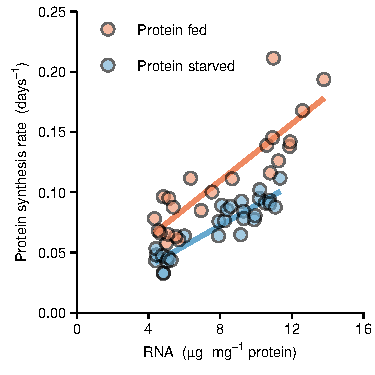
\includegraphics{thesis_files/figure-latex/Millward1973-1} 

}

\caption[Relationship between RNA content and protein synthesis in rat skeletal muscle, data from (160)]{Relationship between RNA abundance and protein synthesis in rat skeletal muscle. Rats were either starved or fed a protein rich diet stimulating protein synthesis. Data from (160).}\label{fig:Millward1973}
\end{figure}
The available data from acute studies on protein synthesis in humans suggests that resistance training leads to muscle hypertrophy through the accumulative effect of repeated bouts of anabolic stimuli. In recent years, this view has been supplemented by evidence suggesting that chronic resistance training also leads to increased rates of protein synthesis at rest
(154, 161, 162),
which has been postulated to be associated with an accumulation of ribosomes, i.e.~an increased translational capacity
(162, 163).
Training-induced increases in muscle RNA abundance support this notion.
As the RNA pool to a large degree consists of ribosomal RNA
(164, 165),
total RNA can be used as a surrogate measure of ribosomal abundance.

\hypertarget{mtorc1-a-multifaceted-coordinator-of-cell-growth}{%
\subsection{mTORC1, a multifaceted coordinator of cell growth}\label{mtorc1-a-multifaceted-coordinator-of-cell-growth}}

The discovery of an organic compound called rapamycin in the 1960s led to the characterization of a rapamycin-sensitive protein involved in cell growth. The protein was later named mechanistic target for rapamycin (mTOR)
(166).
mTOR is found in two protein complexes (mTOR complex 1, mTORC1; mTOR complex 2, mTORC2) where primarily mTORC1 is sensitive to rapamycin treatment
(166).
Bodine \emph{et al.} performed a comprehensive characterization of mTORC1-mediated skeletal muscle hypertrophy using rodent models, showing that mTORC1 activation was essential for load-induced hypertrophy. Additionally, using transfection techniques, they showed that constitutively activated signaling upstream of mTORC1 (Akt) led to hypertrophy in a mTORC1-dependent manner
(167).
Further utilizing rapamycin in genetically modified mice where mTOR was made rapamycin-resistant, specifically in skeletal muscle cells, confirmed that muscle-fiber specific rapamycin-sensitive mTORC1 signaling was needed to induce muscle hypertrophy in response to mechanical loading
(168).
These mechanistic studies support previous observational evidence connecting mTORC1 signaling to muscle growth in rats
(158),
and more recently, in humans
(20, 169).
Administration of rapamycin in humans has also confirmed that mTORC1 signaling is essential for protein synthesis in the acute phase after resistance training (2 hours) and in response to protein ingestion
(170, 171).
However, extending the time-frame (up to 24 hours), differences in responses to resistance exercise between rapamycin treatment and control conditions were less pronounced
(172).
This attenuated effect could be explained by the lower dosage of rapamycin administered in humans than in animals.
It could also indicate rapamycin-insensitive mechanisms controlling translational efficiency
(173, 174).

mTORC1 functions as a signaling hub by integrating multiple environmental cues to regulate cellular growth. Among such cues is mechanical stimulation, which leads to the accumulation of phosphatidic acid in muscle cells
(175).
Such accumulation was shown to be independent of regulators upstream of mTORC1
(175, 176)
but still readily led to mTORC1 activation
(175, 176), indicating direct stimulation of mTORC1 by phosphaticic acid.
In cellular models, phosphatidic acid has been shown to interact with mTORC1 on the same site targeted by rapamycin
(177).
The enzyme primarily responsible for mechanically induced increases of phosphatidic acid is diacylglycerol kinase \(\zeta\)
(178).
In the context of muscle growth in response to resistance training, adequate supplementation of dietary protein augments responses
(69).
Mechanistically, dietary protein intake increases the availability of amino acids in muscle cells, and these, in turn, stimulate protein synthesis through mTORC1 by multiple mechanisms
(179).
mTORC1 capabilities to fine-tune its response based on cellular status can be exemplified from studies examining responses to different amino acid compositions.
Providing a mixture of essential amino acids potentiated mTORC1 signaling in response to resistance exercise more than the provision of essential amino acids without leucine or leucine alone
(180).
In addition to mechanical stimuli and amino acids, mTORC1 integrates several environmental cues related to growth factors, energy, and oxygen status, with downstream signaling differing depending on upstream signaling and cellular characteristics
(181).

Two well-characterized downstream targets of mTORC1 relay much of its information related to translational control, eIF-4E (eukaryotic translation initiation factor 4E)-binding protein 1 (4E-BP1) and S6 kinase 1 (S6K1).
Upon activation, 4E-BP1 releases eIF-4E
(182)
which enables the formation of a preinitiation complex and subsequent recruitment of the small ribosomal subunit to mRNA
(183).
eEIF-4E-dependent initiation of translation is believed to be rate-limiting and thus a control point for protein synthesis.
Interestingly, the formation of the preinitiation complex, induced by the mTORC1-4E-BP1-mediated release of eIF-4E, results in enhanced translation of a special class of mRNAs, containing a 5' structures that do not permit efficient translation
(183,184).
Among the resulting gene products from such mRNA are growth factors, cell cycle regulators such as cyclin D1 and c-Myc, and ribosomal proteins
(166,183).
Parallel to 4E-BP1 is S6K1 which was named after its ability to phosphorylate ribosomal protein S6 but has since been shown to have multiple roles related to both translational efficiency and indirectly to translational capacity
(166).
The importance of S6K1 in control of muscle mass is apparent from S6K1 depletion in mice, which results in reduced muscle growth. Conversely, constitutively active S6K1 results in increased myotube growth in cell cultures
(185, 186).
This reduced growth could be related to S6K1 deficient mice being unable to induce transcription of genes related to ribosomal biogenesis
(187).
Upon activation of Akt, such mice fail to respond by increasing ribosomal biogenesis, evident as failure to accumulate total RNA and rRNA
(188).
S6K1 activity also leads to phosphorylation of downstream targets that enables translation initiation and elongation in addition to its most well-known substrate ribosomal protein S6 (rpS6)
(189).
Although a target of mTORC1, rpS6 has been shown to have a counterintuitive role in protein synthesis.
Despite its location within the ribosome close to its core, mice genetically modified to be unable to phosphorylate rpS6 upon stimulation still form polysomes indicating that rpS6 phosphorylation is not needed for translation initiation
(190).
Protein synthesis rates in the same mice are also higher compared to wild type mice suggesting an inhibitory role of rpS6 phosphorylation in protein synthesis
(190).
Interestingly, mice depleted of S6K1 showed reduced specific force compared to wild-type mice, coinciding with forming of protein aggregates
(188).
Together these observations point to fine-tuning mechanisms in the S6K1-rpS6-axis, balancing protein synthesis, protein quality, and energy wastage
(188, 190).
Fine-tuning may also exist within the mTORC1-S6K1 axis as S6K1 stimulates mTOR phosphorylation at Ser\textsuperscript{2448}
(191),
a commonly used read-out for mTORC1 activity
(192).
Additionally, mTORC1 signaling is sensitive to training status evident from changes in acute signaling in response to resistance training depending on the acute training status
(189, 193).
After three and six weeks of training, the acute exercise-induced response (60-90 minutes post-exercise) in mTORC1-related signaling is practically abolished in young males
(193).
Similarly, in well-trained participants accustom to resistance training, acute resistance-exercise does not lead to perturbations along the Akt-mTORC1-axis in comparison to endurance-trained participants
(194).
These studies are limited in their temporal resolution as only signaling events in the early recovery phase were investigated.
However, they indicate that exercise-induced mTORC1-signaling is sensitive to aspects relating to training status.

\hypertarget{ribosomal-biogenesis-and-muscle-hypertrophy}{%
\subsection{Ribosomal biogenesis and muscle hypertrophy}\label{ribosomal-biogenesis-and-muscle-hypertrophy}}

Ribosomal abundance is a determining factor for protein synthesis and subsequent cellular and tissue size, as was briefly mentioned above.
In addition to correlations between RNA abundance and protein synthesis in mice
(160)
and cell culture
(195),
inhibition of ribosomal RNA (rRNA) transcription or inhibition of upstream transcription factors act to diminish muscle cell growth upon stimulation
(196,195,197).
In the context of resistance training-induced muscle growth, observational evidence from human studies further supports a determining role of ribosomal biogenesis to achieve increased translational capacity and enable hypertrophy.
Figueiredo \emph{et al.} observed a correlation between the changes in RNA abundance and magnitude of muscle growth over eight weeks of resistance training
(198).
Stec and colleagues observed increased ribosomal RNA and total RNA abundance only in participants that were classified as modest or extreme responders in terms of muscle growth but not low responders after four weeks of resistance training
(196).
Similarly, Mobley \emph{et al.} found larger increases in total RNA in participants classified as high- vs.~low-responders to 12 week resistance training (34\% vs.~8\% increase in total RNA) together with a correlation between total RNA increases and muscle growth over the same period
(199).
Finally, Reidy \emph{et al.} reported a correlation between changes in total RNA content and muscle growth
(162)
Together these studies underline the importance of ribosomal biogenesis and translational capacity in resistance training-induced muscle hypertrophy.
However, it should be noted that protein synthesis and cellular growth may occur in the absence of ribosomal biogenesis.
In cultured myotubes stimulated with IGF-1, inhibition of ribosomal RNA transcription led to reduced RNA content but not reduced myotube size compared to non-inhibited controls
(200).
In aged male participants, three sessions of resistance training did not lead to increased levels of RNA but a 30\% increase in protein synthesis rates
(201).
Furthermore, in response to a higher number of training sessions, absence or reduced ribosomal biogenesis is observed in selected individuals, but muscle growth may still be detected
(193).
However, when comparing aged and young skeletal muscle, aged muscle typically respond with reduced hypertrophy after mechanical stimuli, coinciding with reduced ribosomal biogenesis
(193,202),
indicating that potent ribosomal biogenesis is needed to support greater hypertrophy.
Similarly, when comparing cell culture experiments, a ``broader'' stimuli induced by serum compared to a single growth factor could induce greater cellular growth that subsequently requires the support of an increased translational capacity
(200, 197, 196).

Markers of \emph{de novo} synthesis of ribosomes are indeed a hallmark of the early response to resistance training as a single resistance-exercise session leads to increases in precursor rRNA (pre-rRNA 45S)
(203,204)
and repeated bouts lead to accumulation of rRNA/total RNA and thus presumably functional ribosomes
(203, 205, 196,198, 193, 162).
The time course of ribosomal transcription and accumulation in response to resistance training in humans remains largely unknown, with only a few studies investigating exercise- or training-induced changes in markers of ribosomal abundance over multiple time-points.
For example, two consecutive bouts of electrically evoked muscle contractions were associated with increased levels of total RNA, with peak values being observed 72 hrs after the second bout
(205).
Using voluntary contractions, peak values in total RNA were reported after nine sessions, followed by a slight decrease after 18 sessions (193).
These data suggest that ribosomes accumulate with some delay from initiation of training, reaches a plateau in the early phase of resistance training (three weeks), and slightly decreases as muscle mass further increases
(193,205).

The synthesis of new ribosomes is a complex and energy-demanding process, believed to be determined by the rates of pre-rRNA transcription by RNA polymerase I (Pol I), which in turn is regulated by the coordinated assembly of a complex of transcription factors at the rDNA promoter
(206).
rRNA transcription is coupled with the synthesis of ribosomal proteins and the assembly into functional ribosomal subunits
(207,206, 208).
Three of the four mature rRNA (except rRNA 5S) are derived from a single pre-rRNA transcript (45S pre-rRNA). After being transcribed from ribosomal DNA (rDNA), the 45S pre-rRNA transcript goes through several splicing events, ultimately leading to the formation of three rRNA species, 18S, 5.8S, and 28S. Simultaneously with the splicing of rRNA, modifications to the rRNA structure and assembly with ribosomal proteins into precursor ribosomal subunits occur in the nucleolar compartment
(208).
After export to the cytoplasm, additional maturation steps are required in both subunits before they can form functional ribosomes\\
(208).

Activation of the upstream binding factor (UBF) through phosphorylation is needed to initiate rRNA transcription
(209, 210).
This activation is partly controlled by mTORC1-activity, with its inhibition being associated with decreased UBF phosphorylation and inhibition through association with retinoblastoma protein
(211)
which in turn leads to reduced availability and ability of UBF to recruit secondary factors to the rDNA promoter and stimulate rRNA transcription
(212, 213).
Interestingly, the availability of UBF \emph{per se} has also been shown to be a determinant of rRNA transcription
(214, 213)
through control of rDNA gene activity
(215).
mTORC1 also controls one of these secondary factors, TIF-1A, as rapamycin leads to specific phosphorylation and its translocation away from the nuclei
(216),
in addition to inducing chromatin modulations at the rDNA promoter
(217).

mTORC1 is not the only determinant of rDNA transcription. Specific inhibition of MEK showed that MEK/ERK signaling is essential for UBF binding to rDNA
(218).
Furthermore, the transcription factor c-Myc has also been implicated in ribosomal biogenesis as its inhibition coincides with less UBF activity and rRNA transcription irrespective of mTORC1 signaling
(195).
c-Myc is also found at the rDNA promoter and is required for rDNA transcription
(219, 217),
in addition to its role in transcription of genes imoportant for rRNA transcription, e.g.~UBF
(220).

In summary, ribosomal biogenesis and the regulation of translation are under coordinated control of several pathways integrating multiple stressors and environmental cues to regulate cellular protein synthesis.

\hypertarget{transcriptional-regulation-of-training-induced-muscle-tissue-remodeling-with-analytical-challenges}{%
\subsection{Transcriptional regulation of training-induced muscle tissue remodeling (with analytical challenges)}\label{transcriptional-regulation-of-training-induced-muscle-tissue-remodeling-with-analytical-challenges}}

Skeletal muscle fibers are polynuclear cells. Each fiber contains multiple nuclei, which supports its transcriptional needs. Muscle fiber-specific nuclei (myonuclei) cannot proliferate, and the muscle fiber is therefore relying on dormant cell populations located in muscle tissue to activate and supply the fiber with transcriptional capacity during growth or in response to injury
(221).
Among these cells, satellite cells are the primary source of myonuclear accretion in adult skeletal muscle.
However other cell types may also contribute
(221, 222).
Satellite cells can be activated, proliferate or differentiate and fuse with the muscle fiber upon specific stimuli such as hormonal activation
(223)
or mechanical stress
(224),
or return to their quiescent state
(221).
In humans, satellite cells can be readily activated in response to resistance exercise. Activation that leads to them exiting their quiescent state to proliferate
(225, 226, 227),
which in turn leads to an increased number of satellite cells after resistance training
(228).

A possible growth limiting role for satellite cells in the context of muscle hypertrophy is to maintain a fixed number of myonuclei per muscle fiber volume through myonuclear accretion, in order to maintain transcriptional capacity (a maintained myonuclear domain)
(221).
However, human studies do not necessarily show that such a role would determine hypertrophy.
Kadi \emph{et al.} reported that although the number of satellite cells increased by resistance training, the number of myonuclei did not,
suggesting that existing myonuclei were sufficient to provide transcriptional capacity in hypertrophied muscle
(229).
Similarly, other studies have reported increases in muscle fiber cross-sectional area, without or with minimal increases in the myonuclei pool
(230, 231).
In contrast, Petrella and colleagues reported that extreme responders to 16 weeks of resistance training also increased their myonuclear number more than modest, and non-responders
(232).
However, this analysis may have been confounded by the fact that the clustering did not account for age or sex. For example, the extreme-responder group contained nine young (20-35 years) but only two elderly (60-75 years) male participants whereas the non-responder group contained one young man and six elderly
(233).
This note is important as satellite cell responses to exercise are different between young and elderly
(225).
Indeed, in a different study using a similar clustering-approach as in (232) training did not result in differences in myonuclear addition between different response-clusters in a homogeneous sample in terms of age (and sex)
(199).
A further argument against the idea of a determining role of myonuclear accretion for resistance-training induced hypertrophy comes from studies in mice where initial muscle growth induced by synergist ablation is unaffected by specific depletion of satellite cells
(222).

In humans, the addition of myonuclei paralleled with an increase in global transcription rates from existing myonuclei are likely both contributing to accumulation of total RNA seen after resistance training.
Myonuclear accretion does not, however, seem to be a limiting factor for muscle growth
(199, 222).
Existing myonuclei are thus able to maintain transcriptional requirements during hypertrophy, possibly relating to a large degree of transcriptional reserve capacity in muscle fibers
(234).
Indeed, this reserve capacity of existing myonuclei seems sufficient to induce a global shift in transcription in response to mechanical loading, including both mRNA and rRNA transcription
(235).
Such a shift in global transcription is indeed a determinant of muscle growth as it sets the limit of ribosomal biogenesis and thus the muscle cells' translational capacity (as reviewed above).

Transcriptional changes in response to mechanical loading are quantitative (RNA per unit of tissue mass) and qualitative. Activation and de-activation of multiple transcriptional programs that enable coordinated responses to the specific stimuli effectively change the global mRNA profile.
Such ``programming'' in muscle tissue affects, e.g.~muscle fiber type composition whereby resistance training leads to ``shut-down'' of \emph{MYH1} expression, which codes for the myosin isoform represented in type IIX fibers
(99).
The changed, relative proportions of transcripts coding for myosin composition will after remodeling reflect the resulting phenotype
(100).
Furthermore, transcriptional remodeling of the extracellular matrix is readily affected by resistance training
(236, 120).
Revisiting satellite cells' role, briefly touched upon in a previous paragraph, highlights that the extracellular matrix's remodeling is a shared venture between multiple cell types.
If satellite cells are depleted from the skeletal muscle of mice subjected to long-term mechanical overload through synergist ablation, a fibrous muscle phenotype is developed with accumulated extracellular matrix components
(237).
This observation indicates that a balance between muscle satellite cells, their daughter cells, and fibroblasts enables coordination between myofiber hypertrophy and extracellular matrix remodeling
(237, 238, 117).
Such coordinated remodeling occurs at least partly through direct exosome transfer of regulating RNA between differentiated satellite cells and fibroblasts
(238).

In humans, previous studies investigating transcriptional responses to resistance training have investigated a single resistance-exercise session (236, 120, 239),
repeated bouts
(240)
and chronic resistance training (241, 120, 236, 121)
for changes in transcriptome (``qualitative'') characteristics using large-scale techniques (micro-arrays or RNA-seq).
Generally, these studies show that a bout of resistance exercise in the untrained state results in a transcriptome profile related to structural damage, remodeling, and inflammation
(240).
Long-term adaptations generally involve extracellular matrix remodeling, changes in expression of genes related to energy metabolism
(241, 120, 236, 121).
In addition to descriptive studies, attempts have also been made to associate transcriptome characteristics and degrees of muscle growth
(121, 55, 242),
and muscle function
(243, 244).

Although these studies have broadened our understanding of transcriptional regulation during adaptations to resistance training, they also highlight the intrinsic difficulties of studying a dynamic and stochastic process
(234).
From a methodological point of view, skeletal muscle subjected to resistance training, exhibit large global changes to the RNA pool, and \emph{qualitative} changes to RNA sub-populations (mRNA).
A common assumption in studies of gene expression is the relative stability of most transcripts, as well as a stability between sub-populations of RNA (mRNA vs.~rRNA)
(245, 246).
Such assumptions may not be valid in many situations, including during muscle hypertrophy
(235, 247, 196, 198, 193).
Depending on the technique used for evaluating RNA expression (e.g., qPCR, micro-array, or RNA-sequencing), data normalization during analysis aims to make experimental conditions comparable using some common denominator.
In cell culture experiments, cell number was suggested to be this denominator for transcript abundances in order to account for global changes in transcription
(245).
Despite the fact that some previous investigations, specifically investigating resistance training, have acknowledged a changed total RNA abundance per muscle weight, indicating that a lower amount of tissue is used for analysis from different conditions (trained vs.~untrained muscle)
(120),
transcript counts are commonly expressed as per transcriptome.

In summary, both quantitative and qualitative changes in transcriptional profiles in response to environmental stress are important determinants of the resulting changes in cellular phenotypes. Skeletal muscle hypertrophy may represent a special case, as it is typically associated with global changes in transcription as well as cellular growth. To fully understand such dynamic systems, the first steps should include explicit evaluation of underlying methodological assumptions
(248, 245, 249)

\hypertarget{effects-of-resistance-exercise-volume-on-molecular-determinants-of-muscle-growth}{%
\section{Effects of resistance exercise volume on molecular determinants of muscle growth}\label{effects-of-resistance-exercise-volume-on-molecular-determinants-of-muscle-growth}}

Given that resistance exercise variables can modify training responses such as muscle growth, it is reasonable to assume that these effects are mediated through muscle growth determinants, including protein synthesis rates and molecular transducers such as mTORC1.
Resistance exercise intensity has been evaluated concerning protein synthesis and activation of targets downstream of mTORC1 (4E-BP1 and S6K1).
Kumar \emph{et al.} showed that maximal stimulation of fractional synthetic rate was achieved with intensities greater than 60\% of 1RM, coinciding with signaling events
(250).
The same group subsequently investigated the effect of training volume at an intensity presumably leading to maximal protein synthesis stimulation (75\% of 1RM).
This analysis revealed a volume-dependent dose-response, as a higher volume of leg extension led to greater protein synthesis one hour after exercise and sustained S6K1 phosphorylation up to four hours after exercise
(251).
Further extending the time frame, Burd and colleagues evaluated a single session consisting of either one or three sets with biopsies sampled 5, 24, and 29 hours after exercise. Both conditions led to increased myofibrillar protein synthesis five and 29 hours after exercise, but to a larger extent in response to three sets.
However, volume-dependent regulation of S6K1 was only seen at 29 hours after exercise, with earlier events (\textless{} 5 hours) possibly missed due to biopsy sampling timing.
No clear volume-dependency was seen in p90RSK1 (downstream of ERK) or rpS6, however eukaryotic initiation factor 2B (eIF2B\(\epsilon\)) phosphorylation was reduced only in the three-set condition at five hours post-exercise (20), presumably mediating translation initiation, although its exact role is still unclear
(252).
Volume-dependent regulation of S6K1 at Thr389 and rpS6 at Ser235/236 were reported 30 minutes after exercise by Terzis \emph{et al.} as six sets of 6RM bilateral leg press resulted in greater phosphorylation compared to three and one set
(21).
No clear differences between volume conditions were seen in Akt at Ser473, mTOR at Ser2448, ERK 1/2 at Thr202/Tyr204, p38 (\(\alpha\),\(\alpha\) and \(\delta\)) at Thr180/Tyr182, p38\(\gamma\) Thr180/Tyr182 or AMPK at Thr172
(21).
Corroborating previous observations regarding exercise volume-dependence of the S6K1-rpS6-axis, Ahtiainen and colleagues also found greater phosphorylation of S6K1 at Thr389, rpS6 at Ser235/236 and Ser240/244 30 minutes after exercise with ten compared to five sets of 10RM leg press.
Furthermore, ERK1/2 at Thr202/Tyr204 and p38 at Thr180/Tyr182 phosphorylations were not found to be volume-dependent
(22).
However, in contrast to Terzis \emph{et al.}, they reported volume-dependence in exercise-induced phosphorylation of AMPK\(\alpha\) at Thr172, this together with AS160 at Thr642, IRS-I Ser636/639 and Akt at Ser473 together with a tendency in LKB1 at Ser428, all related to cellular energy status, glucose uptake and metabolism
(22,253)

Collectively, although limited in precision due to small sample sizes (n = 8-19) and temporal resolution and
these studies points to volume dependency in exercise-induced S6K1\textsuperscript{Thr389} phosphorylation, potentially further augmented when increased number of sets are examined in the acute phase
(\textgreater{} 3 sets, \textless{} 5 hours; (20,147) vs. (21,22,251)).
Increased S6K1 phosophorylation coincides with rpS6\textsuperscript{Ser235/236} and \textsuperscript{Ser240/244} in the acute phase (\textless{} 5 hours) after exercise
(21,22) but not in the late phase (29 hours) (20).
Although rpS6\textsuperscript{Ser235/236} is a known substrate for both S6K1 and ERK1/2 and p90RSK1
(254),
ERK1/2\textsuperscript{Thr202/Tyr204} was not found to be volume-sensitive in the acute phase
(21,22),
nor was P90RSK1\textsuperscript{Thr573} in the late phase (20)
suggesting that signaling along the mTORC1-S6K1-rpS6-axis is more sensitive to variable volume than the parallel MEK/ERK-axis.
The above signaling events suggest exercise volume-dependent activation of the translational machinery, and increased volume indeed leads to increased muscle protein synthesis
(20,251).
However, relatively high exercise volumes may lead to signaling events inhibiting protein synthesis as AMPK\textsuperscript{Thr172} showed volume dependency, presumably relating to cellular energy stress and glucose metabolism
(22,253, 255).
Interestingly, an increased AMPK-related signaling may be related to an accumulated effect due to short inter-set rest periods, coinciding with reduced proteins synthesis, at least in the acute phase after exercise
(256).

In addition to the signaling events described above, training-induced satellite cell activation has been shown to be volume dependent.
Hanssen \emph{et al.} found that training with three sets compared to a single set per exercise led to a more pronounced increase in cells positive for the satellite cell marker CD56 in \emph{m. vastus lateralis} at two and twelve weeks of resistance training (257).
This coincided with a greater number of myonuclei after 12 weeks of training, although without apparent differences between volume conditions.
In the same muscle specimen, no clear volume-dependent effect was seen on muscle fiber CSA. However, on the muscle level, a positive effect of three- compared to one-set was seen for muscle hypertrophy.
(146,257)

\hypertarget{aims}{%
\chapter{Aims}\label{aims}}

This thesis's primary aim was to relate the adaptive response to resistance training with low- and moderate-volume to skeletal-muscle characteristics in previously untrained individuals. The key question was whether manipulation of exercise volume will have different effects in different individuals and if this variability was associated with individual characteristics. A further aim was to characterize exercise volume dependence in molecular muscle characteristics and determine a time course profile of ribosomal biogenesis markers in response to resistance training. Based on these aims, the objectives were;
\begin{itemize}
\tightlist
\item
  to associate skeletal muscle and systemic characteristics to the benefit of moderate- compared to low-volume resistance training.
\item
  To determine volume-dependence in molecular networks related to muscle growth and remodeling in response to resistance training, and,
\item
  to determine a time course of markers related to ribosome biogenesis in the early phase of resistance training.
\end{itemize}
\hypertarget{methods}{%
\chapter{Methods}\label{methods}}

\hypertarget{study-overview}{%
\section{Study overview}\label{study-overview}}

Study I was designed to examine effects of low- (a single-set per exercise) and moderate-volume (three sets per exercise) on responses to acute exercise and long-term training within participants.
A schematic overview of Study I can be seen in Figure \ref{fig:study1-overview}.
Before the training intervention, participants reported to the laboratory for bilateral baseline muscle biopsies (\emph{m. vastus lateralis}).
Bilateral muscle biopsies were also sampled before and 60 minutes after the fifth training session and after the intervention (Figure \ref{fig:study1-overview}).
Assessments of muscle strength (unilateral isokinetic and isometric knee extension torque as well as unilateral knee extension and leg press one repetition maximum) were performed twice at baseline and further measured in weeks 3, 5, 9, and after the intervention (Figure \ref{fig:study1-overview}).
Body composition measurements (magnetic resonance imaging and dual-energy X-ray absorptiometry) were performed at baseline and after the intervention.

Study II was designed to study the effects of resistance training \emph{per se} and effects of variable compared to constant inter-session volume on selected markers related to ribosome biogenesis.
Participants were therefore recruited to an experimental group and a non-training control group.
An overview of Study II can be seen in Figure \ref{fig:study2-overview}.
Baseline muscle strength (unilateral isokinetic and isometric knee-extension torque) was assessed during three initial visits to the laboratory, with the last baseline-assessment performed at least seven days before the first biopsy sampling. Follow-up measures of muscle strength in the experimental group were completed three and nine days after the last training session.
Muscle thickness (\emph{m. vastus lateralis}) was measured bilaterally before the study and two and eight days after the last training session in the experimental group.
Muscle biopsies were sampled bilaterally before any training, 48 hours after the first, fourth, fifth, eighth, ninth, and twelfth session and eight days after the twelfth session (Figure \ref{fig:study2-overview}).
The control group in Study II performed the same initial assessments as the experimental group. Muscle thickness was again assessed after a control period of 2-4 weeks.
Follow-up muscle biopsies were sampled from one leg 48 hours after the first biopsy as well as after the control period. Follow-up strength assessments were performed 24 hours after the last biopsy.
\begin{figure}

{\centering 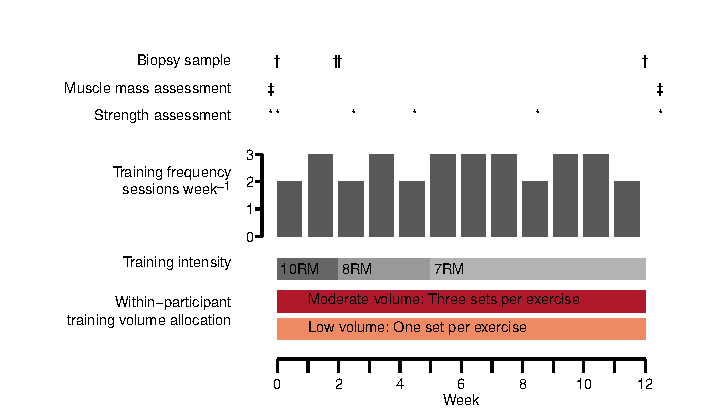
\includegraphics{thesis_files/figure-latex/study1-overview-1} 

}

\caption[Study I, schematic overview]{Schematic representation of Study I, see text for details.}\label{fig:study1-overview}
\end{figure}
\begin{figure}

{\centering 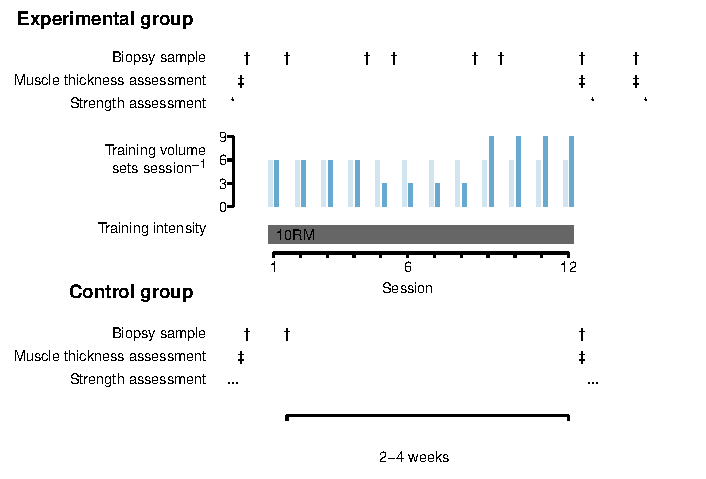
\includegraphics{thesis_files/figure-latex/study2-overview-1} 

}

\caption[Study II, schematic overview]{Schematic representation of Study II, see text for details. }\label{fig:study2-overview}
\end{figure}
\hypertarget{participants}{%
\section{Participants}\label{participants}}

Recruitment to both studies was done through advertising and word of mouth, primarily at Lillehammer University College/Inland University of Applied Sciences. Potential participants were interviewed and matched against inclusion and exclusion criteria. During initial interviews, participants were informed of the study design and time requirements. Participants were also informed about potential risks and sources of discomfort associated with the study before giving their informed consent.

Participants had to be young to be eligible for participation in both studies (Study I age 18-40; Study II 18-35) and non-smoking. Both men and women were eligible for participation. Exclusion criteria included a training history of more than one weekly session during the last 12 (Study I) or six (Study II) months leading up to the study. Participants were also screened for intolerance to local anesthetic, current or previous injuries affecting their ability to perform resistance training, self-reported symptoms or history of disease, intake of medications or supplements with known effects on adaptations to training.
Participant characteristics for both studies are shown in Table
\ref{tab:characteristics-table}.

Forty-one participants were recruited to Study I, and 34 of these completed at least 85\% of the prescribed sessions and were thus included in subsequent data analyses. Reasons for not completing the intervention included injury not related to the study (\emph{n =} 1), pain or discomfort during exercises (\emph{n =} 5), and non-adherence to the study protocol (\emph{n =} 1). There were no systematic differences in characteristics between participants included in or excluded from data analysis in Study I. Before the study, all participants reported that they had previously been engaged in sporting activities. Twenty participants reported regular physical activities at enrollment ranging from once every other week to four times per week. Ten participants reported performing resistance-type exercises at enrollment; however, this was limited to no more than once a week.

Twenty-two participants were recruited to Study II. Three participants did not complete the intervention due to scheduling difficulties. Participants reported familiarity with physical activity but no current systematic resistance training.
\begin{landscape}\begin{table}

\caption{\label{tab:characteristics-table}Participant characteristics}
\centering
\fontsize{7}{9}\selectfont
\begin{tabular}[t]{lllrlllll}
\toprule
  &   & Sex & n & Age (years) & Stature
(cm) & Mass (kg) & Fat mass (\%) & Lean mass (\%)\\
\midrule
 &  & Female & 18 & 22.0 (1.3) & 168 (7) & 64.4 (10.4) & 34.1 (5.6) & 64.3 (6.2)\\
\cmidrule{3-9}
 & \multirow{-2}{*}{\raggedright\arraybackslash Included} & Male & 16 & 23.6 (4.1) & 183 (6) & 75.8 (10.7) & 20.4 (6.0) & 79.3 (5.0)\\
\cmidrule{2-9}
 &  & Female & 4 & 22.9 (1.6) & 166 (8) & 64.6 (9.7) & 28.8 (8.7) & 68.6 (9.1)\\
\cmidrule{3-9}
\multirow{-4}{*}{\raggedright\arraybackslash Study I} & \multirow{-2}{*}{\raggedright\arraybackslash Excluded} & Male & 3 & 24.3 (1.5) & 189 (5) & 88.2 (22.4) & 24.3 (15.3) & 76.8 (12.7)\\
\cmidrule{1-9}
 &  & Female & 6 & 23.4 (2.9) & 168 (8) & 64.0 (9.2) & 30.8 (7.1) & 65.5 (6.8)\\
\cmidrule{3-9}
 & \multirow{-2}{*}{\raggedright\arraybackslash Training} & Male & 5 & 25.7 (5.8) & 177 (3) & 77.5 (8.0) & 25.3 (3.9) & 71.3 (2.4)\\
\cmidrule{2-9}
 &  & Female & 4 & 24.1 (3.5) & 166 (4) & 63.8 (0.6) & 30.5 (6.4) & 66.3 (5.2)\\
\cmidrule{3-9}
\multirow{-4}{*}{\raggedright\arraybackslash Study II} & \multirow{-2}{*}{\raggedright\arraybackslash Control} & Male & 4 & 25.5 (5.5) & 182 (5) & 76.5 (7.7) & 18.2 (5.1) & 78.7 (4.2)\\
\bottomrule
\multicolumn{9}{l}{\rule{0pt}{1em}Data are means and (SD)}\\
\end{tabular}
\end{table}
\end{landscape}
\hypertarget{ethical-approvals}{%
\subsection{Ethical approvals}\label{ethical-approvals}}

Both studies were conducted according to the Declaration of Helsinki
(258).
Studies were approved by the local ethics committee (Study I, no. 2013-11-22:2; Study II, no. 2017-10-23), the Norwegian centre for research data (Study I, 36930/3/LB; Study II, 51549/3/AH), and were pre-registered (Study I, ClinicalTrials.gov Identifier: NCT02179307; Study II, DOI 10.17605/OSF.IO/WA96Y).

\hypertarget{resistance-training-interventions}{%
\section{Resistance training interventions}\label{resistance-training-interventions}}

Studies were performed as within-participant studies
as each participant had their legs assigned to different training
conditions (not including the control group in Study II). Allocation was
performed after enrollment, where each participant had their legs
randomized to either low- or moderate volume (Study I, see Figure \ref{fig:study1-overview}) or variable or constant volume (Study II).

Each training session started with a light, standardized warm-up (5 min
ergometer cycling and ten repetitions each of push-ups, sit-ups,
back-extensions and squats). Before each exercise in the main program,
one set of 10 repetitions were performed in the specific exercise with
approximately 50\% of 1RM.

In Study I, unilateral exercise was performed with a low-volume protocol consisting of a single set of each exercise and a moderate-volume program consisting of three sets per exercise.
Three unilateral leg exercises were used (leg press, leg curl, and knee
extension). The moderate-volume leg commenced all sessions, and the contralateral leg performed a single set of each exercise in the rest between the second and third set of the moderate volume training protocol.

In Study II, unilateral knee-extension was performed. The constant-volume leg performed six sets of 10RM throughout the study. The variable-volume leg performed six sets in session one to four, three sets in session five to eight, and nine sets in session nine to twelve with the same relative intensity (see Figure \ref{fig:study2-overview}).

In both studies, participants performed leg-exercise as part of a full-body program with upper-body exercise performed with two sets after leg-exercises. Upper-body exercises included bilateral bench-press, pull-down, and either shoulder press or seated rowing.

\hypertarget{muscle-strength-assessments}{%
\section{Muscle strength assessments}\label{muscle-strength-assessments}}

Muscle strength was assessed as one repetition maximum (Study I) and isometric and isokinetic torque (Study I and II). In Study I, maximal values from each assessment and time-point were used in statistical analyses, including two separate assessments at baseline, separated by at least four days. For final analyses, a combined muscle strength index was calculated as the average of all tests (1RM, isometric and isokinetic), with all test types given equal weight (expressed as \(\frac{x_i}{max(x)}\) where x is a strength-measure for each leg and time-point (\(i\))). Eighteen participants performed strength assessments at week two, five and nine in addition to baseline and post-training assessments. Training sessions were prioritized for the remaining participants when illness or scheduling difficulties prevented both strength assessment and training.

In Study II, the maximal values from all successful tests sessions at each time-point were used in statistical analyses. Strength assessment sessions were separated by at least 48 hours from preceding training sessions.

\hypertarget{one-repetition-maximum}{%
\subsection{One-repetition maximum}\label{one-repetition-maximum}}

One repetition-maximum (1RM) was assessed in unilateral leg-press and knee-extension in Study I.
Each exercise was assessed after a specific warm-up (ten, six, and three repetitions at 50, 75, and 85\% of the anticipated maximum). Attempts were made with increasing resistance (four to six attempts), and the one-repetition maximum was defined as the highest resistance successfully lifted through the full range of motion.

\hypertarget{isokinetic-and-isometric-maximal-torque}{%
\subsection{Isokinetic and isometric maximal torque}\label{isokinetic-and-isometric-maximal-torque}}

Maximal isokinetic and isometric unilateral knee-extension strength was determined using a dynamometer (Study I: Cybex 6000, Cybex International, Medway USA; Study II: Humac Norm, CSMi, Stoughton, MA, USA).
After a brief warm-up (5 min ergometer cycling, RPE 12-14), participants were secured at the hip and shoulders in the dynamometer with the knee joint aligned to its rotation axis.
Individual settings were recorded and used in subsequent measurements.
Participants were familiarized with the test protocol by performing three sub-maximal efforts at each angular speed.
In Study I, three angular velocities were used to determine isokinetic torque (60\(^{\circ}\), 120\(^{\circ}\) and 240\(^{\circ} ~\times\) sec\(^{-1}\)), in Study II an angular velocity of 90\(^{\circ} ~\times\) sec\(^{-1}\) was used for this purpose.
In Study I, participants performed two attempts at 60\(^{\circ} ~\times\) sec\(^{-1}\) and three attempts at 120 and 240\(^{\circ}~\times\) sec\(^{-1}\).
In Study II, three attempts were made at the designated angular velocity.
In both studies, attempts within each angular speed were performed in immediate succession.
After isokinetic testing, the lever was fixed at 30\(^{\circ}\) (full extension \(=90^{\circ}\)), participants were instructed to push with maximal effort for 5 seconds, and the maximal isometric torque was recorded.
Two attempts were made for maximal isometric torque in Study I, and a single attempt was made in Study II.
Sixty seconds of restitution was given between each measurement in both studies, except for between isometric contractions in Study I, where a 30 second restitution period was used.

In subsequent assessment sessions, the first measurement was performed on alternate legs.
In Study II, the dynamometer allowed for participants to remain seated for assessments of both legs. This was not possible in Study I as the measurement system required participants to be re-seated for assessment of the contralateral leg.

\hypertarget{measures-of-muscle-mass}{%
\section{Measures of muscle mass}\label{measures-of-muscle-mass}}

In Study I, muscle mass was measured by magnetic resonance imaging (MRI) and dual-energy X-ray absorptiometry (DXA) before and after the intervention. Both MRI and DXA measurements were completed during the same visit to the laboratory. Participants were instructed to refrain from strenuous physical activity during the last 48 h leading up to the measurements. Post-intervention measurements were completed at least 48 hours after the last strength testing session. Participants were asked to refrain from food consumption for 2 hours leading up to the measurements.

MRI images were obtained from the mid-thigh and analyzed by the same investigator blinded for time (pre- and post-training) and condition (low- and moderate-volume). Multiple images were used to estimate the extensor muscles' cross-sectional area at the same distance from the knee joint.

In Study II, \emph{m. vastus lateralis} muscle thickness was measured by B-mode ultrasonography (SmartUs EXT-1M, Telemed, Vilnius, Lithuania) using a 39 mm 12 MHz, linear array probe. Between each image acquisition, the probe was relocated to the same position. The position was marked on a soft transparent plastic sheet used to relocate the same position in subsequent measurements.
At least three images were captured and quantified for each leg per time-point with values averaged in analyses. Images were analyzed in ImageJ Fiji (259) by a single assessor, blinded for study conditions and time-points.

\hypertarget{muscle-tissue-sampling}{%
\section{Muscle tissue sampling}\label{muscle-tissue-sampling}}

Muscle samples were obtained under local anesthesia (Study I, Xylocaine,
\SI{10}{\mg\per\ml} with adrenalin \SI{5}{\micro\gram\per\ml},
AstraZeneca, Oslo, Norway; Study II, Lidocaine Mylan, \SI{10}{\mg\per\ml}, Mylan Ireland Ltd, Ireland) with a fine needle (12-14 gauge; Universal-plus, Medax, Italy) operated with a spring-loaded instrument (Bard Magnum, Bard Norway AS, Norway). Sampling was performed as previously described (260), with modifications. Anesthesia was injected in the subcutaneous tissue, with care taken not to inject anesthesia into the muscle itself. Following pilot experiments, we decided not to use an insertion cannula as described in (260) as the biopsy needle itself could be used to puncture the skin and muscle fascia. This approach also resulted in less discomfort. Several passes through the same skin puncture were made to obtain sufficient material for downstream analyses. A smaller needle (14 vs.~12 gauge) was used to further minimize discomfort in Study II where more biopsies were sampled over a shorter time span, with exception from when material was used for immunohistochemistry (not presented in this thesis). The first biopsy was
sampled at one-third of the distance between the patella to the \emph{anterior superior iliac spinae} with subsequent biopsies sampled \(\sim\)\SI{2}{cm} proximal to previous samples. In Study II, samples obtained more than one week apart were sampled with closer proximity and distally from previous samples but never at previous sampling sites. The wet muscle weight of aliquots was measured at the collection and used in subsequent analyses.

\hypertarget{immunohistochemistry}{%
\section{Immunohistochemistry}\label{immunohistochemistry}}

In Study I, a portion of each sample was selected for immunohistochemistry analysis. Samples were placed in formalin for fixation (2-4 days) and further processed using a Shandon Excelsior ES (2.5 hours, Thermo Scientific, USA). Samples were sectioned in \SI{4}{um} transverse sections. Orientation was confirmed prior to subsequent specific staining. In case of obvious misalignment, samples were re-oriented and sectioned. Muscle fiber types were determined on sections double-stained with BF-35 (\SI{5}{\micro\gram\per\milli\litre}, Developmental Studies Hybridoma Bank, deposited by Schiaffino, S.) targeting all myosin heavy-chain types except Type IIX, and MyHCSlow (1:4000, catalog M8421L, Sigma-Aldrich Norway AS, Oslo, Norway) specifically targeting myosin heavy-chain Type I.
Antobodies were visualised using BMU UltraView DAB (BF-35) and UltraView Red (MyHCSlow, Ventana Medical Systems, Inc.~Tucson, USA).
Muscle fibers were counted as Type I (red), Type IIA (brown), Type IIX (unstained) or Type IIA/IIX hybrid fibers (light-brown, see Figure \ref{fig:myhc-fig}). Hybrid fibers were analyzed as 0.5 \(\times\) Type IIA and 0.5 \(\times\) Type IIX
(100).

\hypertarget{total-rna-extraction}{%
\subsection{Total RNA extraction}\label{total-rna-extraction}}

Total RNA was extracted from frozen muscle samples using a protocol modified from
(261)
with Trizol reagent (Life Technologies).
Muscle tissue was homogenized in \SI{300}{ul} Trizol with mechanical disruption achieved by Zirconium Oxide Beads (0.5 mm, Next Advance, Inc., New York, USA) and a bead mill (Bullet blender, Next Advance). External, non-mammalian RNA (Lambda PolyA External Standard Kit, Takara Bio Europe, Saint-Germain-en-Laye, France) was added with the initial volume of Trizol to enable per-weight normalization in subsequent analyses. After homogenization, additional Trizol was added to a total volume of \SI{1}{ml}. Phase separation was achieved by centrifugation after the addition of chloroform (\SI{200}{ul}). The upper phase (\SI{400}{ul} in Study I; \SI{450}{ul} in Study II) was transferred to a fresh tube, and RNA was precipitated using isopropanol (\SI{500}{ul}). After incubation (10 min, room temperature) and centrifugation (12000 g, 10 min at 4\(^{\circ}\)C), the resulting RNA pellet was washed three times in chilled 75\% ethanol.

As previously mentioned, to minimize discomfort due to a greater number of biopsies sampled over a short time, a smaller needle was used for most biopsies in Study II. This generally led to less tissue used for RNA extractions. However, samples from both studies followed the same association between sample weight and Total RNA content (Figure \ref{fig:rna-muscle-weight-methods}a). Further comparing studies using pre-intervention biopsies indicate comparable RNA per tissue-weight readings across the two studies (Figure \ref{fig:rna-muscle-weight-methods}b).
\begin{figure}

{\centering 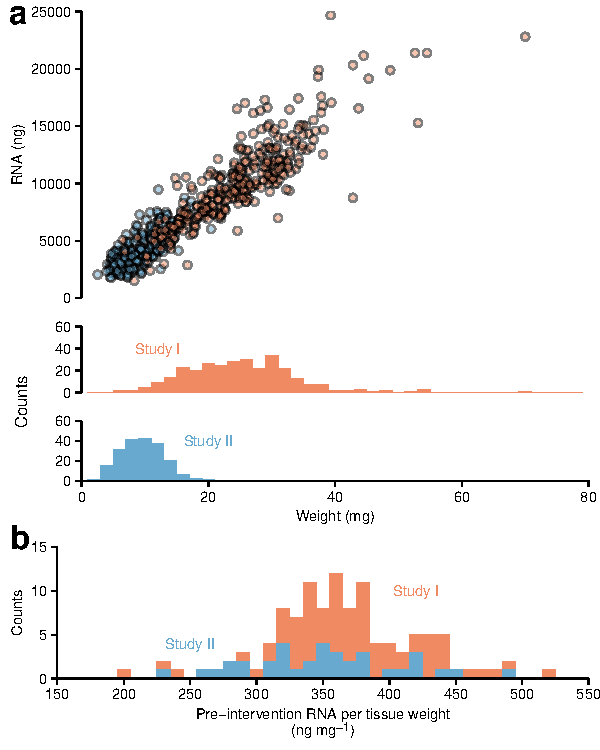
\includegraphics{thesis_files/figure-latex/rna-muscle-weight-methods-1} 

}

\caption[Characteristics of total RNA extracted per study]{Characteristics of total RNA extracted per study and relationship with muscle weight (a). Distribution of pre-intervention RNA per tissue weight (ng mg\textsuperscript{-1}) (b)}\label{fig:rna-muscle-weight-methods}
\end{figure}
\hypertarget{protein-extraction-and-immunoblotting}{%
\section{Protein extraction and immunoblotting}\label{protein-extraction-and-immunoblotting}}

In Study I, muscle-tissue (\(\sim\) \SI{25}{mg} wet weight) was homogenized using a plastic pestle in ice-cold lysis buffer (2 mM HEPES pH 7.4, 1 mM EDTA, 5 mM EGTA, 10 mM MgCl\textsubscript{2}, 1\(\%\) Triton X-100) supplemented with protease and phosphatase inhibitors (Halt, Thermo Fischer Scientific, Life Technologies AS, Oslo Norway). Samples were subsequently incubated at \(4^{\circ}\) for 1 hour followed by centrifugation (10 min at 10 000 g and 4\(^{\circ}\)C). Supernatants were collected for total protein quantification using Bradford reagents (Pierce Detergent Compatible Bradford Assay Reagent, Thermo Fischer Scientific).
Samples were normalized in lysis buffer and 4X Laemmli sample buffer (Bio-Rad Laboratories AB, Oslo Norway) containing 2-Mercaptoethanol, heated to 95\(^{\circ}\)C for 5 min and stored at -20\(^{\circ}\)C until further processing.

In Study II, protein was extracted from Trizol preparations following suggestions by Kopec \emph{et al.} (262)
with modifications. After removing the remaining aqueous phase, DNA was precipitated by the addition of \SI{300}{ul} of absolute ethanol and centrifugation (2000 g, 5 min at room temperature). An aliquot of the phenol-ethanol phase, corresponding to \(\sim\) \SI{1.75}{mg} of tissue, was transferred to a fresh tube and at least two volumes of isopropanol were added followed by incubation (10 min at room temperature). After centrifugation (7500 g, 10 min 4\(^{\circ}\)C), a pellet formed and was subsequently washed three times in 95\% ethanol. Each wash was separated by centrifugation (5000g, 5 min at room temperature). Following the final wash, all liquid was removed, and \SI{45}{ul} of Kopec buffer (262) was added (5\% SDS, 10 mM Tris, 140 mM NaCl and 20 mM EDTA, pH 8; containing protease and phosphatase inhibitors).
Pellets were incubated three hours at 50\(^{\circ}\)C, after which nearly all samples were dissolved.
Any undissolved material was sedimented by centrifugation (10000 g, 10 min at room temperature).
Protein concentrations were determined, and samples normalized as described for Study I.

In both studies, \SI{20}{ug} total protein per sample was separated by gel eletrophoresis (250-300 V for 30-50 min using 4-20\% gels, Criterion TGX, Bio-Rad), and transferred to PVDF membranes (300 mA for 3 hours, \SI{0.2}{um} Immun-Blot, Bio-Rad).
Membranes were stained for total protein using a reversible total protein stain (Pierce Reversible Protein Stain, ThermoFischer Scientific) to ensure transfer and enable protein quantification.
Membranes were blocked for two hours in blocking buffer (tris-buffered saline, TBS, 20 mM Tris, 150 mM NaCl) containing 3\% bovine serum albumin or 5\% skimmed milk and 0.1\% Tween-20.
Incubation with primary antibodies was done over-night, followed by 1-2 hours incubation with secondary antibodies.
Membranes were washed in TBS containing \(0.1\%\) Tween-20 for 3-8 \(\times\) 5-10 min after incubation with the primary antibody, and for 4-8 \(\times\) 5-10 min after incubation with secondary antibodies.
Chemiluminescent detection was used to quantify relative target protein abundance (SuperSignal™ West Femto Maximum Sensitivity Substrate, ThermoFischer Scientific).
For selected targets, following chemiluminescent detection, membranes were incubated with hydrogen peroxide (15 min, 37\(^{\circ}\)C) to inactivate the horseradish peroxidase (HRP), as described by Sennepin \emph{et al.} (263), enabling detection of other epitopes using antibodies from different hosts (mouse or rabbit).
Incubation and wash steps were either performed in an automated fashion at \(4^{\circ}\)C (BlotCycler, Precision Biosystems, Mansfield, MA, USA), or by hand at room temperature with incubations at \(4^{\circ}\)C.
Total-protein content, defined as the mean grey value of the whole well, was quantified with ImageJ (264). Quantification of between-well gray values was subtracted as background. Image Studio Lite (LI-COR Biotechnology, Lincoln, Nebraska USA) was used to quantify chemiluminescence signals. Primary antibodies used in both studies are presented in Table \ref{tab:primary-antibodies-table}.
\begin{table}

\caption{\label{tab:primary-antibodies-table}Antibodies used in immunoblotting.}
\centering
\fontsize{7}{9}\selectfont
\begin{tabular}[t]{lllll}
\toprule
 & Target & Host & Manufacturer & Cat-nr\\
\midrule
 & mTOR\textsuperscript{Ser2448} & Rabbit &  & 5536\\

 & pan-mTOR & Mouse &  & 4517\\

 & p85 S6K1\textsuperscript{Thr412} & Mouse &  & 9206\\

 & p70 S6K1\textsuperscript{Thr389} & Rabbit &  & 9234\\

 & pan-S6K1 & Rabbit &  & 2708\\

 & rpS6\textsuperscript{Ser235/236} & Rabbit &  & 4858\\

 & pan-rpS6 & Mouse & \multirow{-7}{*}{\raggedright\arraybackslash Cell Signaling Technology} & 2317\\

\multirow{-8}{*}{\raggedright\arraybackslash Primary} & pan-UBF & Mouse & Santa-Cruz Biotechnology & sc-13125\\
\cmidrule{1-5}
 & Anti-mouse IgG &  &  & 7076\\

\multirow{-2}{*}{\raggedright\arraybackslash Secondary} & Anti-rabbit IgG &  & \multirow{-2}{*}{\raggedright\arraybackslash Cell Signaling Technology} & 7074\\
\bottomrule
\end{tabular}
\end{table}
\hypertarget{rna-analysis}{%
\section{RNA analysis}\label{rna-analysis}}

\hypertarget{quantitative-real-time-reverse-transcription-polymerase-chain-reaction-qpcr}{%
\subsection{Quantitative real-time reverse transcription polymerase chain reaction (qPCR)}\label{quantitative-real-time-reverse-transcription-polymerase-chain-reaction-qpcr}}

Complementary DNA (cDNA) was synthesized in duplicates from \SI{500}{ng} of total RNA using Superscript IV (Thermo Fisher Scientific) was used according to the manufacturer's instruction. Random hexamer and anchored Oligo-dT primers (Thermo Fisher Scientific) were used to enable quantification of mRNA and rRNA.
SYBR-green-based master mixes (2X SYBR Select Master Mix or PowerUp™ SYBR™ Green Master Mix, Thermo Fisher) were used together with diluted cDNA (\SI{2}{ul}, 1:25-50 dilution) and target-specific primers (\SI{500}{nanomole}) in \SI{10}{ul} total reaction volumes. Detection of light emitted from PCR reactions was captured with a real-time detection system (Applied Biosystems 7500 fast Real-Time PCR Systems or QuantStudio 5 Real-Time PCR System, Thermo Fisher Scientific). Fast cycling over 40 cycles was used adopted to each master-mix. Melt curves and agarose gel electrophoresis were used to confirm single product amplification, product sizes, and no amplification in experiments without a template.
In-house, target-specific primers were designed using Primer-BLAST (265), Primer3Plus (266). Primers targeting the external RNA control were supplied with the kit. Several primers per target were designed and subsequently assessed for their performance. Primers with confirmed single-product amplification and with the lowest threshold cycle for each target were used in analyses.

Raw fluorescence data were exported from the real-time detection system and modeled with a best-fit sigmoidal model.
Wrapper functions for the qpcR-package (267) was written to streamline the process
(\href{http://www.github.com/dhammarstrom/qpcrpal}{github.com/dhammarstrom/qpcrpal}).
Threshold cycles (Ct) were estimated from the models by the second-derivate maximum method with technical duplicates modeled independently (267).
Amplification efficiencies were estimated from every amplification curve
(267,268),
and the mean amplification efficiency (\(E\)) per primer was used to transform amplification data to the linear scale (\(E^{-Ct}\)).

Gene expression data was log-transformed before statistical analysis and modeled as per total RNA,
or per tissue weight using the external RNA and tissue weight as the normalization factor.
In both cases, a random effect per every technical duplicate was used to perform model-based normalization as suggested by Matz \emph{et al.}
(269), with slight modifications. In Study I, log-transformed data were fitted to mixed linear models using the \texttt{lme} function in the \texttt{nlme} package
(270).
This allowed for the combined analysis of a set of genes while accounting for per-target heterogeneity of residual variance. The residual variance could additionally be modeled with Ct-values as a variance covariate using variance functions
(270),
accounting for larger errors at higher Ct-values.
In Study II, a Bayesian analog to this approach was used, more similar to what was described by Matz \emph{et al.}
(269).
Here qPCR-data was transformed to counts (269) and modeled in Poisson generalized mixed linear models using the \texttt{MCMCglmm} package
(271).
In Study I, RNA integrity was assessed by capillary electrophoresis (Experion Automated Electrophoresis Station using RNA StdSens Assay, Bio-Rad).
As Ct-values, but not efficiencies are related to RNA integrity (272),
integrity scores were incorporated in the statistical treatment of qPCR data as fixed effects to control for potential degradation effects for each target, as suggested by
(269).

\hypertarget{rna-sequencing-library-preparation-and-bioinformatic-treatment}{%
\subsection{RNA sequencing, library preparation and bioinformatic treatment}\label{rna-sequencing-library-preparation-and-bioinformatic-treatment}}

\hypertarget{illumina-library-preparation-and-sequencing}{%
\subsubsection{Illumina library preparation and sequencing}\label{illumina-library-preparation-and-sequencing}}

mRNA sequencing libraries were prepared from a fixed amount of RNA (typically 1000 ng, depending on the minimum amount available per participant). cDNA synthesis was performed with TruSeq Stranded Total RNA Library Prep (Illumina, San Diego, CA USA). Subsequent sequencing was performed as 150 bp paired-end sequencing using an Illumina HiSeq 3000 (Illumina) at the Norwegian Sequencing Centre.

\hypertarget{read-quantification}{%
\subsubsection{Read quantification}\label{read-quantification}}

Discarding low-quality reads and trimming of poor-quality bases was done using default settings before alignment (Trim Galore, version 0.6.5, \url{https://github.com/FelixKrueger/TrimGalore}; Trimmomatic, version 0.39 (273)). Filtered reads were subsequently aligned to the human genome (GRCh38 release-97) using several methods, including alignment-based methods
(HISAT2, version 2.1.0 (274); STAR, version 2.7.2 (275); and
RSEM, version 1.3.1 (276),
used together with Bowtie 2, version 2.3.4.3 (277)),
and non-alignment based methods (kallisto, version 0.44.0 (278);
Salmon, version 0.13.1 (279)).
The use of several quantification tools enabled customization of the bioinfomatic pipeline (see \ref{methodological-considerations}).

\hypertarget{modeling-of-gene-counts}{%
\subsubsection{Modeling of gene counts}\label{modeling-of-gene-counts}}

Gene counts were modeled in a single statistical framework (negative binomial generalized linear mixed models, GLMM), as suggested by Cui \emph{et al.} (280).
Modifications were made to account for the particular study design and three different normalization approaches wherein tissue weight and library size were accounted for. Tissue weight was included as an offset term, and library sizes were modeled as a fixed effect.
An additional model without any normalization was used for comparisons.
These models were used in all samples obtained at rest. However, acute phase biopsies (1 hour after the fifth session) were only modeled using the library size as the normalization factor. It was not likely that the amount of tissue used in sample preparation would change in this short time span as no large fluctuations in total RNA to tissue weight were to be expected
(281).
We did, however, suspect that fluid shifts could influence the estimation of tissue weights
(282).
Library sizes were expressed as the effective library size and calculated as the product of the total library size and the RNA composition normalization factor
(246).
Effective library sizes were subsequently divided by the median effective library size, as suggested by Cui \emph{et al.}
(280).

\hypertarget{functional-annotation}{%
\subsubsection{Functional annotation}\label{functional-annotation}}

Gene ontology gene sets were used in enrichment analyses
(283,284),
performed using three approaches.
First, A non-directional rank test based on the gene-specific lower/upper limit of the 95\% confidence interval around the log fold-change. When the log fold-change was greater than 0, the lower limit was used. When the log fold-change was lesser than 0, the negative inverse of the upper 95\% CI was used
(285--287).
Second, directional regulation of the gene sets was assessed using gene-set enrichment analysis
(288,289) with log fold-change as the gene level metric.
Third, over-representation analysis was performed to assess if genes identified as differentially expressed (\textbar fold-change\textbar{} \textgreater{} 0.5, false discovery-rate adjusted \emph{P}-values \textless{} 0.05) belonged to specific gene sets
(290){]}.
The parallel use of a combination of gene set analysis methods utilizing different directionality has previously been proposed as a way to improve the interpretability of such analyses
(291).
Gene ontology gene sets (biological process, cellular component, and molecular function) were downloaded from the molecular signature database (version 7.1) (292).

\hypertarget{blood-variables}{%
\section{Blood variables}\label{blood-variables}}

In Study I, blood variables were analyzed in venous samples collected at five time-points; before muscle biopsy sampling and 10 minutes after completing the fifth training session. Samples were collected in serum-separating tubes, kept at room temperature for 30 min followed by centrifugation (1500 g, 10 min). Serum was aliquoted and stored at -80\(^{\circ}\)C until analysis.
Total testosterone, cortisol, growth hormone, and insulin-like growth-factor 1 (IGF-1) were measured on an Immulite 1000 analyzer (Siemens Medical Solutions Diagnostics, NY, USA). Vitamin D (S-25-OH-D) levels were measured in samples collected before and after the intervention using an immunoassay (Roche Cobas Vitamin D total assay, Roche Diagnostics GmbH., Mannheim, Germany).

\hypertarget{meta-analysis-of-resistance-training-volume-dependent-effects-on-muscle-mass-and-strength}{%
\section{Meta-analysis of resistance training volume-dependent effects on muscle mass and strength}\label{meta-analysis-of-resistance-training-volume-dependent-effects-on-muscle-mass-and-strength}}

\hypertarget{literature-search-inclusion-criteria-and-coding-of-studies}{%
\subsection{Literature search, inclusion criteria and coding of studies}\label{literature-search-inclusion-criteria-and-coding-of-studies}}

The first set of studies was selected based on inclusion in previously published
meta-analyses (24,25). For more recent studies, PubMed, Google Scholar, and SportDiscuss searches were made with search terms being ``training volume'', ``resistance training'', ``strength training'', ``set'',
``muscle strength'', ``muscle hypertrophy'' used in different combinations. Studies examining the effect of within-session training volume on muscle strength and mass, with all other training variables kept constant between study groups, were considered for inclusion in the meta-analysis.
Studies were further assessed for inclusion based on criteria being; (i) participants described as healthy without medications affecting muscle
metabolism, (ii) interventions lasted at least six weeks, and (iii) resistance training performed without additional stimuli (e.g., blood flow restriction) at intensities greater than 65\% of 1RM or 20RM.

All available outcome measures of muscle mass and strength gains in
response to resistance training were extracted from each study except for outcomes reported as both summaries and individual measures (e.g., muscle thickness reported as individual muscles and summarized for the whole muscle group). In such cases, the summary was used as the outcome. Weekly training volume was calculated as product of weekly sessions, number of sets, and exercises for each muscle group assessed for muscle hypertrophy or strength gains. An intervention-average of weekly sessions was used when the number of sessions per week differed over the course of the intervention. An exercise was assumed to influence an outcome when it targeted prime movers also assessed for strength or muscle hypertrophy measures.
Measures of muscle mass were considered specific if they estimated muscle mass in muscles considered affected directly by exercises. Measures of muscle strength were considered specific when tested in the same exercises as used during training. Measures of muscle mass and strength were identified as targeting the upper-, lower- or whole body.
Participant characteristics were coded based on sex (male, female or mixed when a study failed to discern between males and females), age (young, \textless{} 30 years; middle-aged, 30-50 years; old, \textgreater{} 50 years; or mixed), training status (trained, \textgreater{} 1 session per week during the last six months leading up to the intervention; untrained \textless{} 1 session). Study groups were considered independent also in studies utilizing within-participant models.

\hypertarget{calculations-of-effect-sizes-and-statistical-analysis}{%
\subsection{Calculations of effect sizes and statistical analysis}\label{calculations-of-effect-sizes-and-statistical-analysis}}

Group-wise effect sizes were calculated for each outcome measure based
on the within-group change score pre- to post-training divided by the
pre-training standard deviation (SD). Pre-training SD's were calculated
as a pooled SD within outcome and study. Variances of the effect size
were calculated using an average effect size across all outcomes within
muscle strength or mass, and correlations specific to each measurement
type (isokinetic-, isometric- or repetition maximum strength tests;
muscle thickness, magnetic resonance imaging, dual-energy X‐ray
absorptiometry) estimated from previous studies.
A correction factor (Hedges' g) was applied to both effect sizes and their
variances
(293)

From 25 studies, a total of 151 and 181 effect sizes were coded for muscle mass and strength measurements, respectively. Mixed-effects meta-regression models were used to model the effect of the weekly number of sets on training-induced muscle mass and strength gains.
Confounding variables (age, sex, study length, training status, body portion, and specificity of measurement) were included in all models. Interaction between weekly number of sets and each of the confounding variables were assessed in separate models.
Models were fitted in a Bayesian framework using the brms-package
(294,295).

\hypertarget{statistics-and-data-analysis}{%
\section{Statistics and data analysis}\label{statistics-and-data-analysis}}

In Study I, \emph{a priori} sample-size calculations (\(\beta=20\%\), \(\alpha=5\%\)) indicated that 40 participants were sufficient to detect \(\sim\) 3\% and 5\%-point differences between volume conditions in primary outcomes, training-induced changes in muscle cross-sectional area, and maximal voluntary strength, respectively. Sample-size calculations were based on assumed differences between volume conditions corresponding to effect sizes of 0.47-0.51, as estimated from previous studies (146,147).

In Study II, an initial sample size calculation was made based on a best-case scenario. Data from Brook et al. (296) indicated that a within-participant differences in RNA per tissue weight of \(15\%\) could be detected with seven participants in the experimental group (e.g.~2.79 (0.65) to 3.21 (0.74) \SI{}{\micro\gram\per\micro\litre}, \(\alpha<0.05\), \(\beta<0.2\), effect size = 1.2). The control group was included in the study as a negative control primarily for systems validation of experimental procedures regarding measures of e.g., ribosomal biogenesis. With a balanced design accounting for drop-outs, eight participants were required in each group. After a preliminary analysis of the experiment (experimental group \emph{n = }7, control group \emph{n = }7)(297), additional participants (experimental group \emph{n =} 4, control group \emph{n = }1) were recruited to the study to increase the precision of estimates, primarily in analyses within the experimental group.

In Study I, pre- to post-intervention measures of muscle mass and strength were analyzed as change-scores, modeled with pre-intervention values entered in models as a covariate together with sex, when appropriate. A general model formulation representing the study design was used in analyses of volume-dependent effects. It included time and the time by volume-condition interaction, as suggested by Fitzmaurice \emph{et al.} (298).
The general formulation was used in different models, depending on outcome measure and expected error distributions.
Linear mixed-effects models were used for continuous variables.
Fiber type distributions were analyzed as a proportion of the total number of fibers/transcripts in each sample and thus bound between 0 and 1. Binomial and beta-binomial models were used to account for this in generalized linear mixed-effects models.
The beta-binomial model accounts for the fact that the gene-family-based fiber type distribution has an arbitrary denominator.
Random effects were included when appropriate, and any such structure was reduced to retain a parsimonious model. Exclusion of random effects was made based on their contribution to the model using likelihood ratio tests.
Null-hypotheses of no differences between volume-conditions and no effect of time were tested from model estimates of from linear and generalized mixed-effects models.

In Study I, within-participant differences between volume conditions were used to construct binary response variables representing additional benefit of moderate- over low-volume training in muscle hypertrophy (measured from MRI) and average strength (measured as the weighted average of strength tests). An additional benefit of moderate-volume training was defined as a difference between volume conditions larger than the smallest worthwhile change in the direction of moderate-volume. The smallest worthwhile change was defined as the between-participants SD \(\times\) 0.2. Mean-centered data per sex were used to account for sex differences in CSA and strength measures.
Response variables were related to a wide range of predictors using logistic regression following (299). \emph{A priori} selection of relevant predictor variables was made before modeling. These included blood variables, baseline strength and muscle mass, volume-dependent measures of total-RNA content, and S6K1 phosphorylation expressed as a percentage of low-volume training and baseline fiber-type composition. Additionally, pre-study training characteristics and in-study training variables were included in analyses.
Each possible predictor was assessed in univariate analysis, controlling for sex, and a non-conservative threshold (\(P < 0.20\)) was used to select variables for further modeling.
Predictors were sequentially removed from a full model based on significance tests (\(P > 0.1\)), with models refitted after each removal to assess its influence on other predictors. After model reduction, all removed predictors were added to models to assess their contribution when controlling for predictors identified in primary model reduction. Predictors were checked for linearity (logit) through design variables visual inspection. Non-linear variables were categorized. Thirty-two participants were included in variable selection as two participants had missing data in some of the pre-selected variables.
In this text, secondary analyses were performed using continuous difference-scores between volume conditions and univariate analyses performed with robust regression, accounting for sex when appropriate through mean centering of variables.

In Study II, the effect of training on study outcomes was assessed in linear mixed-effects regression models, fitted in a Bayesian framework.
Time and group (training vs.~control) were treated as fixed effects in analyses with matching time points (all post-intervention data from the training group was used).
Interactions between groups were estimated as \(\Delta\) training - \(\Delta\) control.
The effects of different volume-conditions and general time-course patterns were assessed using all observations in the training group.
Segmented regression models were used to estimate changes over sessions in three segments, sessions 1-4, 4-8, and 8-12, corresponding to different volume prescription blocks in the training group.
Volume-conditions were averaged and presented together when no volume-condition effect was apparent.
Random effects were entered in all models as legs nested within participants.

Individual data, separated per leg, were used to estimate the average increase in total RNA per session throughout the study. Both the rate of increase and the mean RNA abundance was subsequently regressed on change in muscle thickness using a mixed-effects model. Legs nested within participants were used as random effects. Leave-one-out analysis was used to assess the sensitivity of individual observations on associations.

In Study II, inferences were drawn based on point estimates and their 95\% credible intervals (CrI). Credible intervals without the null effect were interpreted as robust. Models were fitted with default priors which also makes CI analogous to confidence intervals. Their interpretation differs as the CrI contains the true population value with the specified certainty (95\%), given the data. Model fitting was considered adequate when at least four different chains of MCMC samples converged (assessed by visual inspection and \(\hat{R}\approx 1\)). Model performance was assessed by comparing simulated data from each model to observed data graphically using posterior predictive checks.

\hypertarget{software-code-and-data-avaliability}{%
\subsection{Software, code and data avaliability}\label{software-code-and-data-avaliability}}

Data analyses were predominantly performed in R (300).
Data wrangling and visualizations were done using packages associated with the
\texttt{tidyverse} (301) and \texttt{ggplot2} (302).
Non-standard statistical models were fitted in
\texttt{nlme} (270),
\texttt{lme4} (303),
\texttt{glmmTMB} (304),
\texttt{brms} (294) and
\texttt{MCMCglmm} (271).

For each paper included in this thesis, data and code are hosted on github (paper 1, \href{https://github.com/dhammarstrom/benefits-of-rt-volume}{github.com/dhammarstrom/benefits-of-rt-volume}; paper 2, \href{https://github.com/dhammarstrom/rnaseq-pipeline}{github.com/dhammarstrom/rnaseq-pipeline};
paper 3, \href{https://github.com/dhammarstrom/ribo-accum-paper}{github.com/dhammarstrom/ribo-accum-paper};
thesis, \href{https://github.com/dhammarstrom/thesis}{github.com/dhammarstrom/thesis}).

\hypertarget{results-and-discussion}{%
\chapter{Results and Discussion}\label{results-and-discussion}}

\hypertarget{muscle-mass-growth}{%
\section{Training volume affects training-induced changes in muscle mass and strength and molecular determinants of muscle hypertrophy}\label{muscle-mass-growth}}

In Study I, the average increases in muscle strength and mass irrespective of volume condition corresponded to what could be expected based on previous research in young, healthy participants (Table \ref{tab:csa-str-tab})
(305, 14),
indicating the general efficacy of the training program.




\begin{table}

\caption{\label{tab:csa-str-tab}Training induced changes in muscle CSA and average strength in Study I}
\centering
\fontsize{7}{9}\selectfont
\begin{tabular}[t]{llll}
\toprule
Sex & Condition & Mean (SD) & Reference\\
\midrule
\addlinespace[0.3em]
\multicolumn{4}{l}{\textbf{CSA \%-change}}\\
\hspace{1em} & LOW & 3.05 (3.61) & \\
\cmidrule{2-3}
\hspace{1em}\multirow{-2}{*}{\raggedright\arraybackslash Female} & MOD & 5.02 (4.04) & \\
\cmidrule{1-3}
\hspace{1em} & LOW & 3.83 (3.50) & \\
\cmidrule{2-3}
\hspace{1em}\multirow{-2}{*}{\raggedright\arraybackslash Male} & MOD & 5.10 (3.71) & \multirow{-4}{*}{\raggedright\arraybackslash }\\
\cmidrule{1-4}
\addlinespace[0.3em]
\multicolumn{4}{l}{\textbf{CSA \%-change per day}}\\
\hspace{1em} & LOW & 0.04 (0.05) & \\
\cmidrule{2-3}
\hspace{1em}\multirow{-2}{*}{\raggedright\arraybackslash Female} & MOD & 0.07 (0.05) & \\
\cmidrule{1-3}
\hspace{1em} & LOW & 0.05 (0.05) & \\
\cmidrule{2-3}
\hspace{1em}\multirow{-2}{*}{\raggedright\arraybackslash Male} & MOD & 0.07 (0.05) & \multirow{-4}{*}{\raggedright\arraybackslash 0.11 [0.04-0.26]a}\\
\cmidrule{1-4}
\addlinespace[0.3em]
\multicolumn{4}{l}{\textbf{CSA \%-change per session}}\\
\hspace{1em} & LOW & 0.11 (0.13) & \\
\cmidrule{2-3}
\hspace{1em}\multirow{-2}{*}{\raggedright\arraybackslash Female} & MOD & 0.18 (0.15) & \multirow{-2}{*}{\raggedright\arraybackslash 0.08 (0.22)b}\\
\cmidrule{1-4}
\hspace{1em} & LOW & 0.14 (0.12) & \\
\cmidrule{2-3}
\hspace{1em}\multirow{-2}{*}{\raggedright\arraybackslash Male} & MOD & 0.19 (0.13) & \multirow{-2}{*}{\raggedright\arraybackslash 0.14 (0.14)b}\\
\cmidrule{1-4}
\addlinespace[0.3em]
\multicolumn{4}{l}{\textbf{Average strength \%-change}}\\
\hspace{1em} & LOW & 21.0 (9.8) & \\
\cmidrule{2-3}
\hspace{1em}\multirow{-2}{*}{\raggedright\arraybackslash Female} & MOD & 27.8 (14.4) & \\
\cmidrule{1-3}
\hspace{1em} & LOW & 19.2 (12.4) & \\
\cmidrule{2-3}
\hspace{1em}\multirow{-2}{*}{\raggedright\arraybackslash Male} & MOD & 23.1 (12.0) & \multirow{-4}{*}{\raggedright\arraybackslash }\\
\cmidrule{1-4}
\addlinespace[0.3em]
\multicolumn{4}{l}{\textbf{Average strength \%-change per session}}\\
\hspace{1em} & LOW & 0.77 (0.36) & \\
\cmidrule{2-3}
\hspace{1em}\multirow{-2}{*}{\raggedright\arraybackslash Female} & MOD & 1.00 (0.49) & \multirow{-2}{*}{\raggedright\arraybackslash 0.67 (0.35)b}\\
\cmidrule{1-4}
\hspace{1em} & LOW & 0.72 (0.48) & \\
\cmidrule{2-3}
\hspace{1em}\multirow{-2}{*}{\raggedright\arraybackslash Male} & MOD & 0.87 (0.46) & \multirow{-2}{*}{\raggedright\arraybackslash 0.47 (0.22)b}\\
\bottomrule
\multicolumn{4}{l}{\textsuperscript{a} Estimates from Wernbom et al. (305)}\\
\multicolumn{4}{l}{\textsuperscript{b} Estimates from Ahtiainen et al. (14)}\\
\end{tabular}
\end{table}
For muscle hypertrophy and strength gains, the moderate-volume condition consistently showed greater adaptations when compared to the low-volume condition (Figure \ref{fig:comb-fig-s1}a).
These patterns were in general agreement with previous meta-analyses indicating that increased training volume leads to more favorable outcomes, both in terms of muscle mass
(25, 24)
and strength
(131, 23).

Since publication of the most recent meta-analyses (25,131),
additional studies have been published investigating the effect of resistance training volume on muscle mass and strength. Based on studies included in the meta-analysis performed by Schoenfeld \emph{et al.} (25), additional results were extracted from studies gathered through a systematic literature search among newly published studies (from January 2015 to June 2020). Compared to Schoenfeld \emph{et al.} (25), an additional ten studies were included in the present analysis.
Subsequently, effect sizes were extracted from 25 studies, both for muscle mass and strength, and meta-regression models were used to investigate the effect of the weekly number of sets on training-induced changes in these outcomes.
Both muscle mass and strength were shown to be robustly affected by an increased training volume measured as an increase in weekly training sets (after controlling for potential confounding factors\footnote{Models were controlled for age (young, middle age or old), sex (male, female or mixed), length of study (number of weeks), type of measurement (direct or indirect for muscle mass and training-specific or unspecific in strength), training status (trained \textgreater{} six months experience with resistance training), body portion (upper, lower or whole)}).
For every additional weekly set, the effect size measure (Hedges' \emph{g}, {[}95\% credible intervals{]} (CrI)), increased by
0.012 {[}0.004, 0.021{]} and 0.021 {[}0.004, 0.037{]}
for muscle mass)
and strength (Figure \ref{fig:comb-fig-s1}b),
respectively.
Together these data underline the training volume dose-dependence of both muscle hypertrophy and strength gains.
\begin{figure}

{\centering 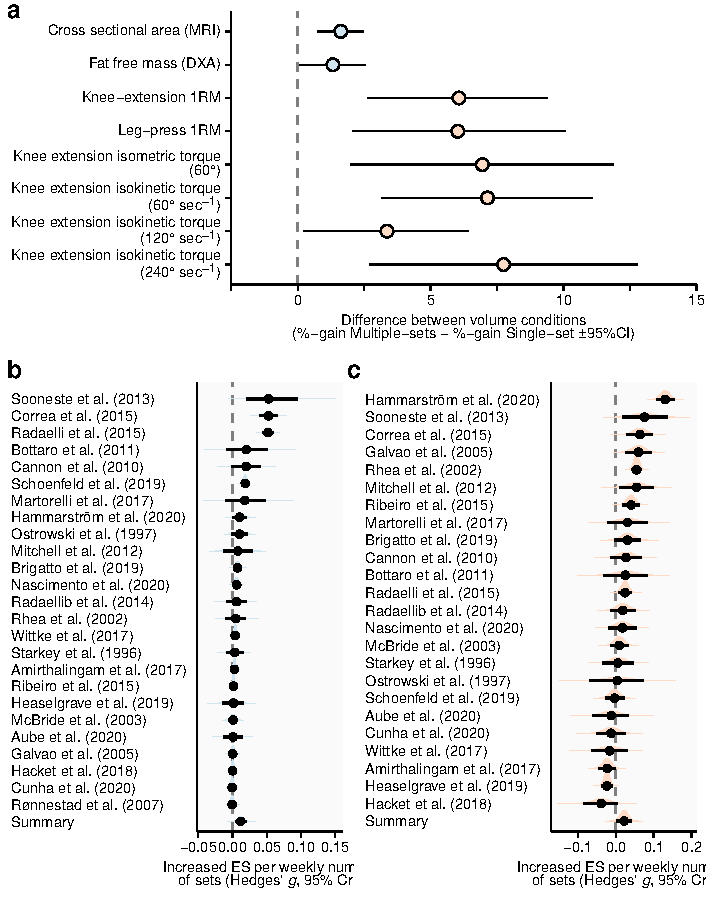
\includegraphics{thesis_files/figure-latex/comb-fig-s1-1} 

}

\caption[Differences in training induced changes to muscle mass and strength measures between volume conditions in Study I and weekly training volume meta-regression.]{Differences in training-induced relative changes in muscle-mass and strength in Study I with estimates derived from ANCOVA models controling for baseline values (a). Estimates from meta-regression models examining the effect of weekly number of sets per muscle group on muscle hypertrophy (b) and strength gains (c). Estimates are effect size measures (Hedges g) with 95\% credible intervals (CrI).}\label{fig:comb-fig-s1}
\end{figure}
In an attempt to explain differences in training outcomes between volume conditions, selected molecular markers known to influence adaptations to resistance training were investigated for volume-dependency.
First, acute activation of signaling along the mechanosensitive mTORC1-pathway was measured before and after the fifth training session in Study I.
A commonly used readout of mTORC1-signaling is the phosphorylation of S6K1 at Thr\textsuperscript{389}/Thr\textsuperscript{412} which in turn precedes phosphorylation of rpS6 (see Figure \ref{fig:mtor-fig}a).
In the present study, exercise induced S6K1\textsuperscript{Thr\textsuperscript{389}/Thr\textsuperscript{412}} phosphorylation was indeed shown to be volume dependent along with phosphorylation of rpS6\textsuperscript{Ser\textsuperscript{235/236}} and mTOR\textsuperscript{Ser\textsuperscript{2448}} (Figure \ref{fig:mtor-fig} b).
Together these observations indicate larger perturbations along the mTORC1 signaling axis which confirms previous studies showing an exercise-volume dependency of mTORC1-related signaling in the acute phase (\textless{} 5 hours) after exercise when the low-volume condition consists of at least three sets
(251, 22, 21, 20,147).
It is recognized that phosphorylation of mTOR itself at Ser\textsuperscript{2448} primarily should be regarded as indicative for negative feedback as this site is phosphorylated due to S6K1 activity
(306) (Figure \ref{fig:mtor-fig} a).
It is also recognized that the phosphorylation status of rpS6 at Ser\textsuperscript{235/236} is not solely due to mTORC1 signaling as both mTORC1 and extracellular signal-regulated kinases (ERK)-signaling converges here
(254).
Interestingly, Terzis \emph{et al.}
(169)
and Ahtiainen \emph{et al.}
(22)
did not report any clear volume dependency in exercise-induced activation of ERK 1/2.
While this may suggest that any volume-dependent regulation of this pathway was outside the timeframe of these studies, it may also suggest that volume selectively modulates specific pathways in the acute phase after resistance exercise.
It should be noted that the present and previous studies are limited in their temporal resolution, and different patterns over time in relation to exercise-volume cannot be ruled out.

The importance of mTORC1 signaling for protein synthesis in the acute phase after resistance exercise is well established.
In humans, administration of rapamycin, a selective inhibitor of mTORC1, before resistance exercise leads to delayed or blunted activation of mTORC1 effectors such as
S6K1 and rpS6, as well as unchanged levels of phosphorylation of 4E-BP1 and eEF2 resulting in abolished exercise-induced increase in protein synthesis
(170).
Volume-dependent increase in mTORC1 signaling also coincide with larger protein synthesis rates
(20, 251)
suggesting that higher exercise volume can be regarded as leading to an increased potential for protein synthesis in the acute-phase after exercise.
Previous studies have indirectly linked mTORC1-related signaling to muscle growth as acute perturbation along this pathway has been correlated with muscle growth
(169, 307).
However, this is not a consistent finding in the literature
(147, 308),
nor is it consistent with the results in the present study as acute activation of S6K1 in response to the fifth session was not associated with training-induced muscle mass changes.\footnote{Raw Spearman's correlations between exercise-induced change in S6K1 phosphorylation and change in muscle mass (measured with MRI) indicated weak (insignificant) associations (\(\rho=\) -0.124 - 0.056) depending on the isoform measured (p70 or p85) and the number of sets. More elaborate modeling confirmed weak relationships between the degree of phosphorylation and muscle mass change. When controlling for baseline values in degree of phosphorylation (as this influence the calculation of fold-change) and number of sets, standardized estimates for the effect of phosphorylation were (increase in \%-muscle mass change for every 1SD change in fold-change phosphorylation, with {[}95\% CI{]}) \(\beta=\) 0.33 {[}-0.53, 1.20{]} for p70 S6K1-p70\textsuperscript{Thr389} and \(\beta=\) -0.51 {[}-1.35, 0.33{]} for S6K1-p85\textsuperscript{Thr412}.}
\begin{figure}

{\centering 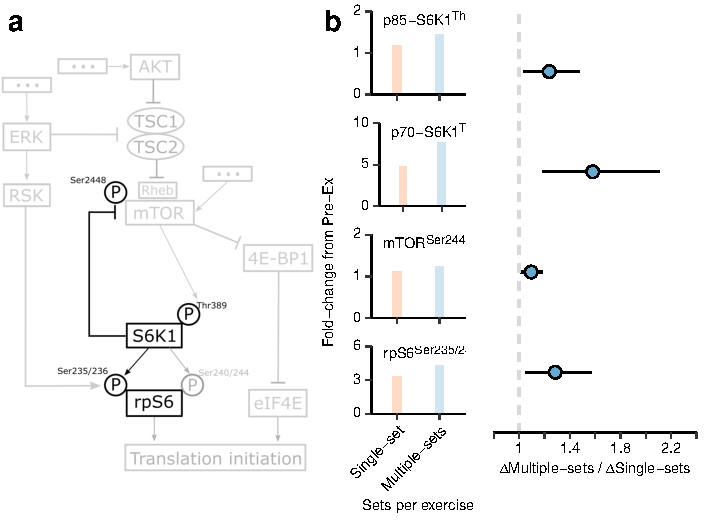
\includegraphics{thesis_files/figure-latex/mtor-fig-1} 

}

\caption[Differences between volume conditions in exercise induced phosphorylation of proteins related to mTORC1 signaling]{Measured phosphorylation sites in context (a) and differences between volume conditions in phosphorylation status of S6K1 at Thr \textsuperscript{389} (p70) Thr \textsuperscript{412} (p85), rpS6 at Ser \textsuperscript{235 236} and mTOR at Ser \textsuperscript{2448} induced by acute exercise and expressed as fold-changes (b). Estimates in b are derived from ANCOVA models controling for baseline values presented as point estimates with 95\% confidence intervals. Dots in a represents up-stream regulators.}\label{fig:mtor-fig}
\end{figure}
Although mTORC1 signaling most certainly contributes to protein synthesis in the acute recovery phase after resistance exercise (170),
several aspects complicate its applicability as a predictor of training-induced muscle hypertrophy.
First, measuring its activity is not straight forward for biological reasons, including pathway cross-talk and negative feedback as well as technical aspects
(192, 254, 309).
Secondly, mTORC1 signaling is not a stable phenomenon either between or within individuals as short- and long-term resistance training leads to diminished activity along its pathway
(193, 194).
Thirdly, mTORC1 readily integrate multiple signals but also convey these to multiple downstream processes
(189).
As such, mTORC1 activity represents an early, transient response to resistance exercise, with its signaling contributing to accumulative responses.
One such downstream target of mTORC1 is ribosomal biogenesis
(212, 197, 217, 187),
ultimately leading to accumulation of ribosomal RNA, a response typically seen in connection with to resistance training
(196,198, 193, 162).

As ribosomal RNA is the most abundant constituent of muscle RNA, it provides an estimate of muscle ribosomal abundance when expressed per unit tissue weight
(164, 160).
From baseline to prior to the fifth training session (Week 2), total RNA per mg tissue increased by \(\sim\) 19 and 34\% in the low- and moderate-volume condition, respectively. Total RNA levels were still elevated above baseline after the intervention (Week 12, low-volume \(\sim\) 13; moderate-volume \(\sim\) 20\%). Similar patterns were seen in target analysis of ribosomal RNA species using qPCR (low-volume increase from baseline to Week 2 \(\sim\) 8-44\% and Week 12 \(\sim\) 14-36\%; moderate-volume \(\sim\) 31-57\% and Week 12 \(\sim\) 14-23\%). Comparing volume conditions revealed higher levels of total RNA and mature ribosomal RNA species in the moderate-volume condition at Week 2 (Figure \ref{fig:rrna-fig}a). At Week 12, between-volume-condition differences in total RNA were less clear and ribosomal RNA 28S even showed higher levels in the low-volume leg (Figure \ref{fig:rrna-fig}a).
Analysis of c-Myc mRNA abundance in response to the fifth training session also showed volume-dependent regulation with exercise-induced increases being \(\sim\) 1.5-fold higher in response to the moderate- compared to the low-volume condition (Figure \ref{fig:rrna-fig}b). c-Myc represents a rapamycin-insensitive signaling pathway, parallel to mTORC1, known to also stimulating ribosomal biogenesis
(195, 219,310).
\begin{figure}

{\centering 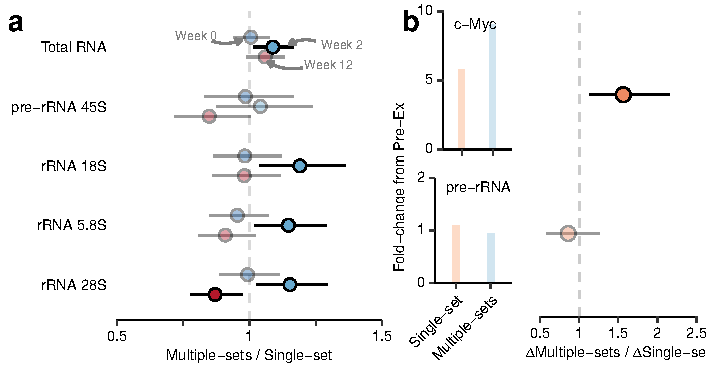
\includegraphics{thesis_files/figure-latex/rrna-fig-1} 

}

\caption[Differences between volume conditions total RNA and ribosomal RNA]{Differences between volume conditions in total RNA and ribosomal RNA-species (pre-rRNA 45S, rRNA 18S, rRNA 5.8S and rRNA 28S) measured at rest at Weeks 0, 2 and 12 in Study I (a). Acute changes in abundance of c-Myc mRNA and pre-rRNA 45S in response to acute exercise in Week 2 and differences between volume conditions (b). Errorbars represents 95\% confidence intervals, transparent points and errorbars signifies that the confidence interval contain 1.}\label{fig:rrna-fig}
\end{figure}
Ribosomal biogenesis is an early adaptation to resistance training with initial increases in total RNA evident before any hypertrophy can be detected
(203, 205, 62, 63).
The increase seen in total RNA serves as a marker of ribosomal accumulation and thus increased translational capacity. This improved translational capacity contributes to protein accretion resulting in muscle hypertrophy, reflected in associations between measures of ribosome abundance (typically total RNA) and muscle hypertrophy
(198, 196, 199, 162).
Due to the sequential nature of these events (increased translational capacity before muscle hypertrophy), early increases in total RNA would possibly better reflect training-induced changes in muscle hypertrophy.
Any increase in muscle mass would also contribute to a dilution of the RNA pool
(281)
possibly masking their causal relationship.
Indeed, comparing the relationships between RNA abundance and muscle hypertrophy at different time-points supported this view as the amount of RNA at Week 2 showed the most robust relationship with the resulting muscle growth (Figure \ref{fig:rrna-csa-fig}, \ref{tab:rna-csa-tab}). This indicates that translational capacity, affected by exercise, early in the training program determines training-induced changes in muscle mass.
\begin{table}

\caption{\label{tab:rna-csa-tab}Influence of RNA abundance on training-induced muscle growth measured with MRI}
\centering
\fontsize{8}{10}\selectfont
\begin{tabular}[t]{lrrrrll}
\toprule
\multicolumn{6}{c}{ } & \multicolumn{1}{c}{Standardized coefficients} \\
\cmidrule(l{3pt}r{3pt}){7-7}
 & Estimate & SE & df & \textit{t}-value & 95\% CI & Estimate [95\% CI]\\
\midrule
(Intercept) & -8.10 & 3.56 & 32 & -2.27 & [-15.35, -0.84] & \\
Moderate- vs. low-volume & 0.67 & 0.41 & 28 & 1.64 & [-0.17, 1.51] & \\
\addlinespace[0.3em]
\multicolumn{7}{l}{\textbf{RNA abundance (ng mg\textsuperscript{-1})}}\\
\hspace{1em}Week 0 & 0.00 & 0.01 & 28 & 0.37 & [-0.01, 0.02] & 0.12 [-0.54, 0.78]\\
\hspace{1em}Week 2 & 0.02 & 0.01 & 28 & 3.58 & [0.01, 0.03] & 1.40 [0.60, 2.21]\\
\hspace{1em}Week 12 & 0.01 & 0.01 & 28 & 1.43 & [-0.00, 0.02] & 0.57 [-0.25, 1.38]\\
\bottomrule
\multicolumn{7}{l}{\textsuperscript{a} Standardized coefficients scaled by its SD}\\
\end{tabular}
\end{table}
\begin{figure}

{\centering 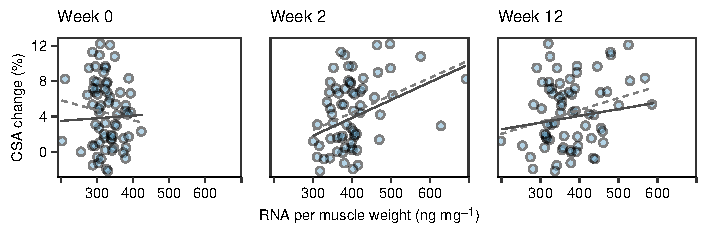
\includegraphics{thesis_files/figure-latex/rrna-csa-fig-1} 

}

\caption[Relationship between total RNA and training induced muscle growth]{Relationship between total RNA and training induced change in thigh cross sectional-area (CSA) as measured by MRI. Dashed line represent naive relationship, solid line represent adjusted reliationship as seen in \\ref{tab:rna-csa-tab}.}\label{fig:rrna-csa-fig}
\end{figure}
\hypertarget{volume-dependent-remodeling-of-muscle-fiber-type-composition}{%
\section{Volume-dependent remodeling of muscle fiber-type composition}\label{volume-dependent-remodeling-of-muscle-fiber-type-composition}}

Resistance training readily leads to remodeling of the muscle, including qualitative changes in fiber type composition through changes in the myosin heavy-chain protein composition
(97, 98, 88, 100).
Resistance training-induced changes in fiber-types identified by myosin heavy-chain expression occurs primarily as a IIX \(\rightarrow\) IIA transition, which results in a more fatigue-resistant phenotype
(88, 99, 93)
and thus represents an important aspect of the adaptive response to resistance training by reversing effects of inactivity and disuse
(101, 102).
In Study I, muscle fiber-type composition was primarily determined based on myosin heavy-chain protein's immunostaining in muscle cross-sections. The staining protocol allowed for the identification of Type I (red), Type IIA (brown), Type IIX (unstained), and Type IIA/IIX hybrids (light brown, Figure \ref{fig:myhc-fig}a). Throughout the study, a general reduction in Type IIX fibers was seen as pure Type IIX was replaced with Type IIA/IIX hybrids at Week 2, and these, in turn, were measured at lower proportions at Week 12 (Figure \ref{fig:myhc-fig}b).

After twelve weeks of training, the proportion of Type IIX fibers was lower in the moderate- compared to the low-volume condition (indicative as an odd-ratio (OR) \textless{} 1, OR {[}95\% CI{]}: 0.54 {[}0.31, 0.94{]}, combined measure of IIX/IIA hybrids and pure IIX fibers, Figure \ref{fig:myhc-fig}d). Reductions seen in Type IIX myosin heavy-chain expression were reflected on the gene level as moderate-volume training led to more pronounced down-regulation of the \emph{MYH1} gene, coding for Type IIX myosin heavy-chain protein, at all time-points during the intervention (Figure \ref{fig:myhc-fig}c).
This observation underlines that training volume is an important factor for fiber-type composition remodeling. Although not surprising, similar observations are lacking in the literature as previous studies have not compared this transition directly between volume protocols.
However, when comparing non-exhaustive high-load resistance training to load-matched training to volatile failure, Pareja-Blanco \emph{et al.}
(311)
observed a blunted IIX \(\rightarrow\) IIA transitions in response to the non-exhaustive protocol.
Together these data indicate that increased metabolic stress and/or dosage of neuromuscular activity are plausible candidates for regulating IIX \(\rightarrow\) IIA reprogramming in humans in response to resistance training.
This as opposed to tensile stimuli.
Based on observations in animal models, neural input might, however, be considered the primary candidate.
For example, in a rat model of resistance training, the force did not affect fast-to-slow fiber-type transitions when performed with the same electrical stimulation pattern, indicating that neural activity governs fiber-type transitions
(224).

At Week 2, a more pronounced reduction in \emph{MYH1} gene abundance in the moderate-volume condition did not translate to the protein level. Instead, a greater number of fibers were classified as IIX in the moderate-volume condition compared to the low-volume condition (OR: 1.56 {[}1.06, 2.32{]}).
The moderate-volume condition thus showed a greater mismatch between gene and protein levels compared to the low-volume condition.
Such mismatch is seen after resistance-exercise and is indicative for the early transition of muscle fibers reflecting the sequential order of events, whereby changes at the RNA level do not immediately translate into changes at the protein level
(99).
This indicated that remodeling occurred faster in response to the low-volume condition despite a greater ``transition signal'' in the moderate-volume leg.
A plausible explanation for this observation could be that the likely more pronounced cellular repair after damage caused by a greater training stimulus leads to a delayed fiber-type transition.
This hypothesis is supported by observations indicating that a proportion of the protein synthesis seen early in a resistance-training period can be attributed to tissue repair rather than myofibrillar synthesis
(154, 312).
Regardless of causality, the more rapid early adaptation seen in response to a lower training volume suggests that optimized resistance training should include a progressive volume component.

\pagebreak
\begin{figure}

{\centering 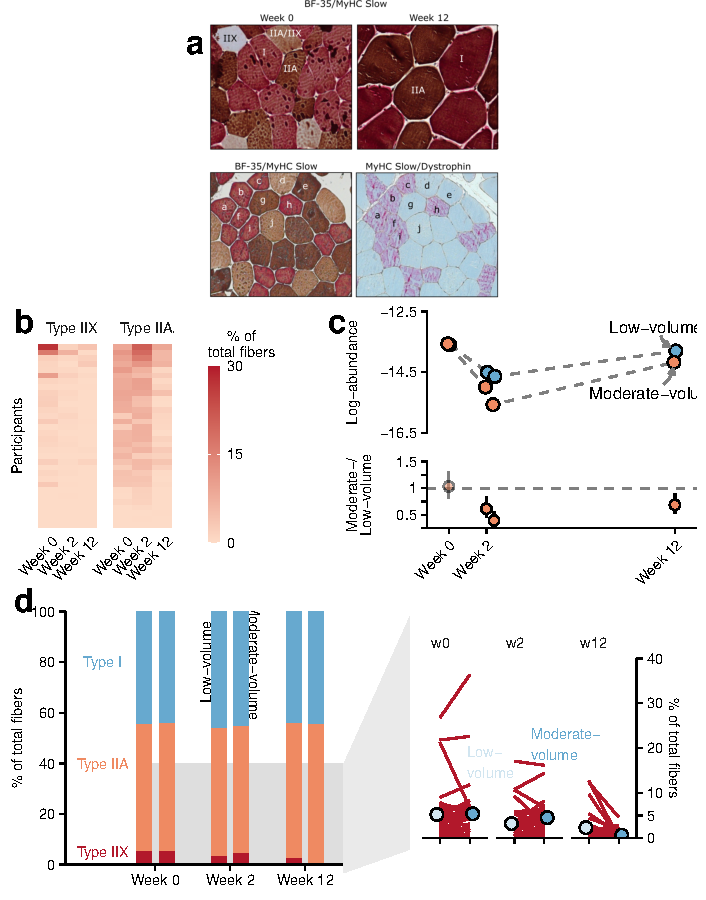
\includegraphics{thesis_files/figure-latex/myhc-fig-1} 

}

\caption[Fiber-type composition in Study I]{Representative muscle cross-sections stained for myosin-heavy chain isoforms are shown in (a). Using antibodies for Type I (MyHC Slow) and all but Type IIX (BF-35) enabeled separating Type I fibres from other fibres (red stain, a lower panel). Type IIX fibers were indentified as unstained, and weak brown staining was analysed as Type IIX/IIA hybrids (a, upper panel). Resistance training led to a reduction in Type IIX and IIX/IIA hybrids, (b) shows participant-average Type IIX and IIX/IIA percentages. Training led to reduction in \textit{MYH1} gene expression, and more so in the moderate-volume condition, evident from pairwise comparisons in (fold-differences with 95\% CI, c). Differeces in protein expression of Type IIX fiber (counted as pure IIX + 0.5 $\times$ IIX/IIA hybrids) reversed throught the study as the moderate-volume condition showed greater proprtions of IIX fibers at Week 2 but lesser expression at Week 12 (d).}\label{fig:myhc-fig}
\end{figure}
\pagebreak

\hypertarget{volume-dependent-effects-on-transcriptome-characteristics}{%
\section{Volume-dependent effects on transcriptome characteristics}\label{volume-dependent-effects-on-transcriptome-characteristics}}

As already \protect\hyperlink{muscle-mass-growth}{discussed}, resistance training in Study I led to an increase in total RNA per unit tissue weight. The magnitude of this increase was different between volume conditions (see Figure \ref{fig:rrna-fig}).
Studies of gene expression using qPCR and RNA sequencing techniques assume that equal amounts of biological material are used when evaluating the abundance of single transcripts.
It is therefore common to use a set amount of total RNA during sample preparation to satisfy such an assumption
(120, 241, 313).
However, if the ratio of RNA to tissue mass for some reason changes throughout the course of a study, this would mean that analyses are performed on different amounts of tissue. This may be the case after a resistance-training intervention, and may even be differentially affected by different resistance training modalities, such as in Study I.
Indeed, in Study I, the resistance training protocol resulted in a situation where samples were prepared from a lesser amount of tissue as a fixed amount of RNA was used during sample preparation.
This effect was more pronounced in response to the moderate- compared to the low-volume condition (Figure \ref{fig:lib-size-fig}a).

Despite the fixed amount of total RNA being used during sample preparation, the total abundance of mRNA increased, evident as increases in total library sizes, quantified from RNA sequencing as the total number of quantified gene counts. The average increase in total library size was more apparent in the low-volume condition
(Figure \ref{fig:lib-size-fig}b).
When library sizes were normalized to the amount of tissue used in sample preparation, differences between conditions were diminished
(Figure \ref{fig:lib-size-fig}c).
This suggests that resistance-training lead to increased global mRNA expression per-unit-muscle weight (43-53\% in the present study). This increase was not different between volume-conditions, suggesting that the volume-dependent regulation of RNA transcription primarily relates to transcription of RNA-fractions such as rRNA rather than mRNA (see Figure \ref{fig:rrna-fig}).
\begin{figure}

{\centering 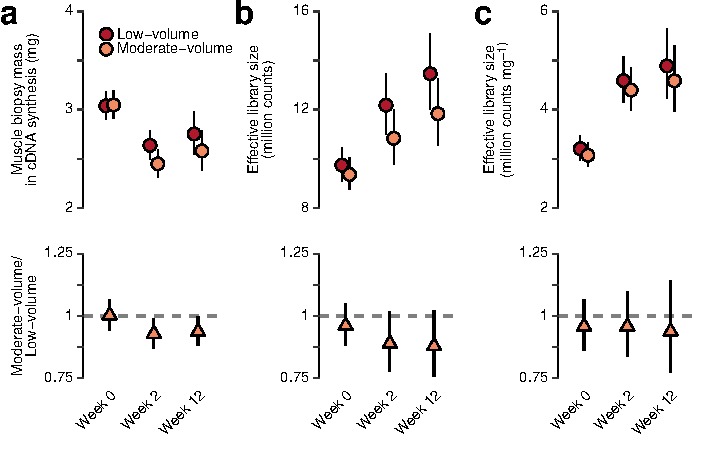
\includegraphics{thesis_files/figure-latex/lib-size-fig-1} 

}

\caption[Muscle weight and RNA-seq library size]{Less muscle tissue was used for cDNA synthesis in the moderat- compared to low-volume condition as a result of total RNA increases per tissue weight (a). Library sizes tended to be greater in the low-volume condition (b), after normalizing library sizes to muscle weight differences were diminished (c). Lower panels shows differences between volume conditions}\label{fig:lib-size-fig}
\end{figure}
Although the observed increase in library sizes suggests global increases in mRNA transcription, it did not resemble global gene amplification seen in models with experimentally manipulated c-Myc protein expression
(247, 245)
as a considerable fraction of genes were unchanged by training.
When expressing gene abundance per the amount of tissue used in sample preparation, 42.1\% and 19.6\% of identified genes were classified\footnote{Up- and down-regulated genes were classified based on log\textsubscript{2}-fold change \textgreater{} 0.5 and \textless{} -0.5 together with FDR-corrected \emph{P}-values \textless{} 0.05} as unchanged from baseline to Week 2 and 12, respectively. A small fraction of genes were identified as being less abundant at Week 2 (0.21\%) and Week 12 (0.01\%). The majority of genes were classified as up-regulated from baseline to Week 2 (57.7\%) and Week 12 (80.4\%).

Gene-set enrichment analyses revealed that training-induced changes in gene expression profiles were related to increased abundance of genes associated with extracellular matrix remodeling, collagen synthesis and inflammatory processes. Although these observations were made without a proper control to investigate training-induced effects \emph{per se}, they resemble previous (controlled and uncontrolled) studies characterizing skeletal muscle tissue in response to heavy mechanical loading in the acute phase
(314, 315, 119, 122),
and after prolonged training (121, 120).
\begin{figure}

{\centering 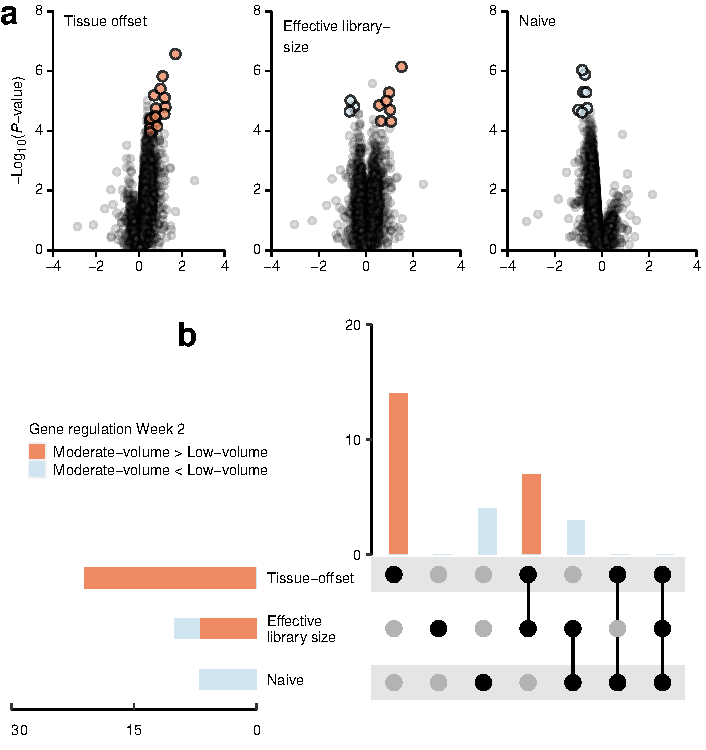
\includegraphics{thesis_files/figure-latex/week2-upset-volcano-1} 

}

\caption[General patterns of differentially expressed genes at Week 2]{Volume dependent differences in gene expression in different models (a) either accounting for the amount of tissue used in cDNA synthesis (Tissue offset), library sizes or un-normalized (Naive). Genes identified as differentially expressed (log2 fold-change > |0.5|, FDR < 0.05) are highlighted in a.  Overlap in differentially expressed genes between models are shown in (b)}\label{fig:week2-upset-volcano}
\end{figure}
To be able to account for differences in the amount of tissue used in sample preparation due to volume-dependent differences in the ratio of total RNA to tissue weight, three different normalization strategies were used to determine volume-dependence in transcriptome characteristics.
By implementing each normalization strategy as variations of generalized linear mixed models (GLMM), we could compare outcomes related to conceptually different normalization techniques using the same statistical framework.
The use of GLMM also had the benefit of accounting for the study design, which included correlated data (within participants)
(280).
In the first model, an offset term expressing gene counts per tissue weight was included. This term was combined with the effective library size, included as a fixed effect in the model together with study conditions, time, and exercise volume (tissue offset-model).
In a second model, the offset term was removed. Thus only the effective library size was used to normalize the gene counts, as suggested by Cui \emph{et al.}
(280) (effective library-size model).
For comparison, a naive model containing no normalization-parameters was also included in analyses.

At Week 2, tissue-offset normalization (modeling mRNA counts per-mg-muscle weight) revealed a general shift of mRNA counts towards the moderate-volume condition (Figure \ref{fig:week2-upset-volcano}a).
This contrasted patterns found using ``conventional'' library-size normalization that in turn more resembled the non-normalized naive model, seen as an overlap of genes identified as differentially expressed between the models (Figure \ref{fig:week2-upset-volcano}b).
Gene-set enrichment analyzes revealed that genes related to extracellular matrix remodeling and collagen synthesis were driving the difference in transcriptome profiles between volume-conditions at Week 2
(Figure \ref{fig:week2-go-analysis}a).
This was apparent using both the tissue offset model and the library-size normalized model. However, the volume-dependent effects were more pronounced in the tissue-offset model
(Figure \ref{fig:week2-go-analysis}b).
Differences in normalization models led to global shifts of estimates of differences between volume conditions. Figure \ref{fig:gene-set-rug} shows this global shift as density curves representing all fold-changes between volume conditions. Accounting for the amount of muscle mass in sample preparations also shifted specific gene-sets towards greater differences between volume conditions. This is exemplified in Figure \ref{fig:gene-set-rug} by the gene set ``Collagen containing extracellular matrix''.
\begin{figure}

{\centering 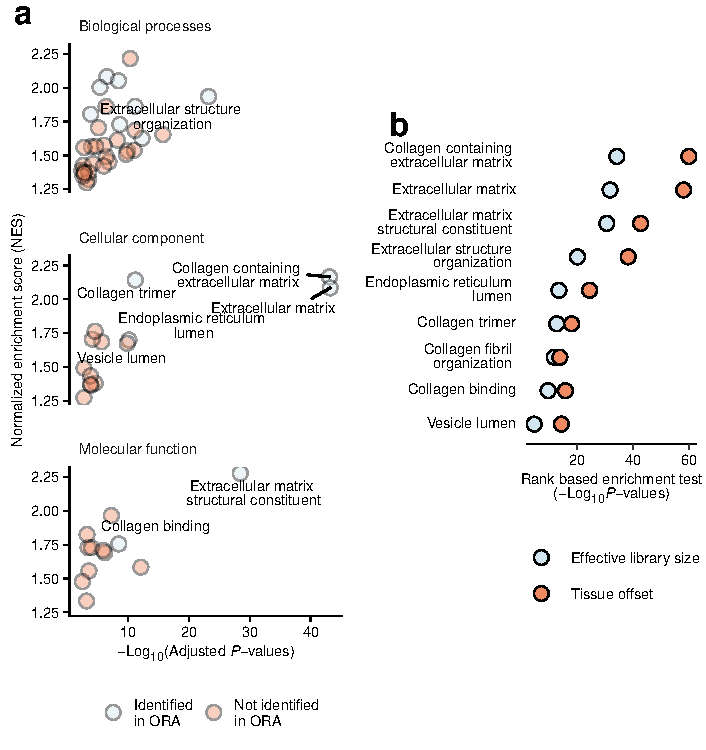
\includegraphics{thesis_files/figure-latex/week2-go-analysis-1} 

}

\caption[Gene-set enrichment analysis at Week 2]{Gene-set enrichment analysis based on gene-ontology gene sets and estimates from the tissue-offset model (a). Adjusted \textit{P}-values and Normalized enrichment scores are retrieved from analysis of directional rank-based tests (GSEA), labeling of points indicate if gene-sets were also identified from differentially expressed genes (Log2 fold-change >|0.5|, FDR < 0.05). In (b) comparison between the tissue-offset and library size normalization models are shown in rank-based (non-directional, cerno-test) analysis of gene ontology gene sets.}\label{fig:week2-go-analysis}
\end{figure}
\begin{figure}

{\centering 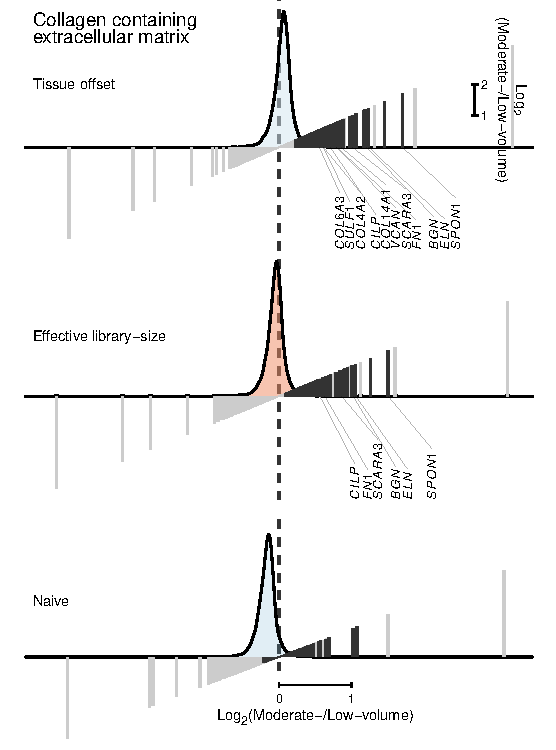
\includegraphics{thesis_files/figure-latex/gene-set-rug-1} 

}

\caption[Global shifts in volume-dependent fold change as an effect of normalization methods at Week 2]{Differences between volume conditions at Week 2 as seen using different normalization models. Shifts in the full distribution of Log2-fold change values between volume conditions were seen between on normalization models (density curves). As an example, genes associated with the \textit{Collagen containing extracellular matrix} gene set are highlighted (black bars), differentially expressed genes are identified with gene symbols in each method.}\label{fig:gene-set-rug}
\end{figure}
At week 12, differences seen at Week 2 between volume conditions derived from the tissue-offset model were abolished (Figure \ref{fig:week12-upset-volcano}a). In contrast, volume-dependent differences were seen in the library-size normalized model with genes identified as having higher expression in the low-volume condition. However, these overlapped with the naive model, indicating that imbalance in muscle tissue between conditions may have contributed to global shifts in favor of the low-volume condition. This indicates that towards the end of the training intervention, the muscle tissue may have reached a new transcriptional equilibrium.
\begin{figure}

{\centering 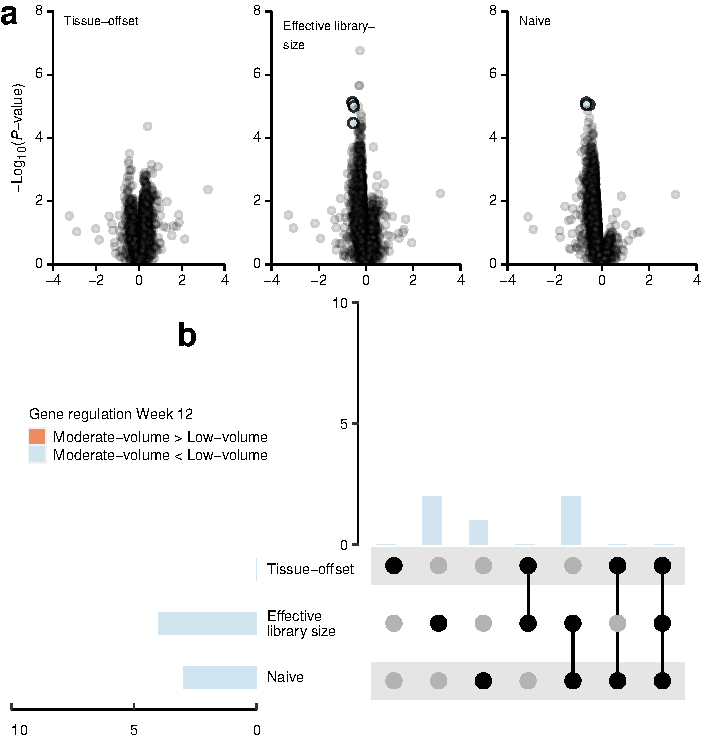
\includegraphics{thesis_files/figure-latex/week12-upset-volcano-1} 

}

\caption[General patterns of differentially expressed genes at Week 12]{Volume dependent differences in gene expression in different models (a) either accounting for the amount of tissue used in cDNA synthesis (Tissue offset), library sizes or un-normalized (Naive). Overlap in differentially expressed genes between models are shown in (b)}\label{fig:week12-upset-volcano}
\end{figure}
From a general perspective, this analysis underlines the importance of a well-considered choice of normalization strategy in studies of gene expression in non-homeostatic conditions
(316, 249, 245).
Specifically, in gene expression studies of training-induced muscle hypertrophy, an ill-advised normalization strategy will mask or overestimate differences between experimental conditions as different amount of tissue is being used in sample preparation. This, as a consequence of a normalized RNA input between different conditions. Differences in the amount of tissue used in sample preparation between volume-conditions in Study I effectively led to underestimating genes identified as differentially expressed at Week 2 and led to nonsensible identification of differentially expressed genes at Week 12.
The choice of normalization strategy ultimately determines the definition of differential expression. By using the tissue offset model, we were interested in gene counts per tissue, as opposed to using the the library size as the denominator in analyses, leading to gene counts expressed per transcriptome. Although both strategies may have merit in certain situations, selected genes may be better studied as counts per amount of tissue. It could be argued that one such group of genes are genes related to extracellular matrix remodeling.
First, extracellular matrix-related genes have been shown to display close association between mRNAs abundances and their respective proteins, including collagen-organization proteins (317).
This indicates that remodeling on the protein level is primarily determined by transcriptional regulation.
Second, selected extracellular-matrix related genes are primarily expressed in other cells than muscle fibers (e.g.~fibroblasts)
(318, 117).
Thus assuming that an increase in total RNA due to increased ribosomal biogenesis would scale to other cell types in muscle tissue might introduce bias to such gene expression data.
Consequently, studies of transcriptional regulation of extracellular matrix remodeling concerning muscle hypertrophy should account for the amount of tissue used in analyses.

Extracellular matrix remodeling have not been found to be affected by different exercise variables. Instead, when comparing low- and high-load, Holm \emph{et al.} found similar responses measured as collagen synthesis (119)..
Similarly, a comparison of concenctric and eccentric resistance training did not reveal differential effects on muscle collagen synthesis
(122).
Although it should be noted that the measures of collagen synthesis and measures of gene expression related to extracellular matrix target different facets of extracellular matrix remodeling, volume-dependent regulation of these target genes implicates this remodeling as paralleled with muscle growth.

\hypertarget{transcriptome-responses-to-acute-exercise}{%
\subsection{Transcriptome responses to acute exercise}\label{transcriptome-responses-to-acute-exercise}}

In Week 2, in response to acute exercise, 4.7 and 6.9\% of identified genes were categorized as up and down-regulated 1 hour after exercise.
These changes were measured as per transcriptome as no change in the total RNA per tissue weight was expected
(281).
Instead, fluid shifts (282)
could be expected to affect analyses in the short timeframe through a biased estimation of wet muscle weight.
The differentially regulated genes were generally associated with stress responses, including inflammation and immune responses and extracellular matrix-related processes. In contrast to the observed changes in response to prolonged resistance training, acute exercise led to down-regulation of extracellular matrix-related genes, similar to what has been found by others (121).

Regarding volume-dependent regulation in the acute phase, only a single gene was found to be differentially expressed between volume-conditions. This gene, \emph{RFT1}, was found to be down-regulated and more so in response to moderate-volume exercise. It is associated with lipid transport, carbohydrate transport, and endoplasmic reticulum membrane and has previously been found to decrease in muscle after exercise (319).
Further analyses of volume-dependent differences not relying solely on arbitrarily defined differential expression confirmed that no robust differences were evident in transcriptome characteristics in this short time-span.
The timing of the post-exercise biopsy likely missed more relevant volume-dependent regulation in the acute phase.

\hypertarget{determinants}{%
\section{Determinants of moderate- over low-volume training benefit}\label{determinants}}

To explore determining factors for the additional benefit of moderate- over low-volume training, individual differences in muscle-hypertrophy (CSA) and average muscle strength between the moderate- and low-volume conditions were calculated. In primary analyses, difference scores were dichotomized to \emph{benefit of moderate-volume training} or \emph{no benefit of moderate-volume training} based on the smallest worthwhile change (SWC) in the direction of moderate volume. Participants were thus identified as having \emph{benefit of moderate-volume training} if the difference in raw change scores were greater than the between-participants baseline SD \(\times\) 0.2 in favor of moderate-volume training.\footnote{Sex-differences were accounted for by mean-centering variables prior to SD estimation. A weighted SWC was calculated for the strength variable to avoid underestimating SD.}
The choice of using a dichotomized response variable (benefit vs.~no benefit) was made to maintain an individual perspective, i.e., irrespective of the magnitude of the individual difference, what determines the benefit of moderate- over low-volume training?
\begin{figure}

{\centering 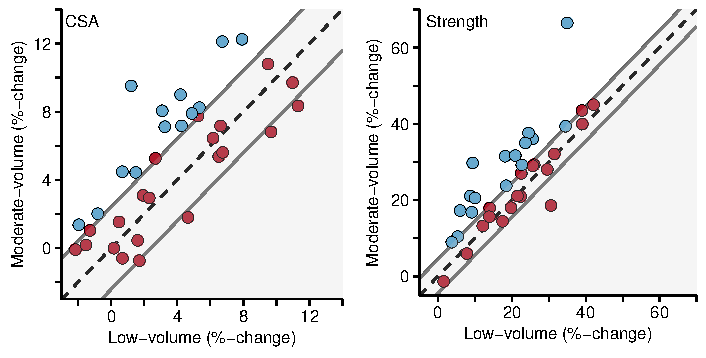
\includegraphics{thesis_files/figure-latex/csa-str-sets-corr-1} 

}

\caption[Relationship between individual responses to moderate- and low-volume training]{Relationship between individual responses to moderate- and low-volume training. Dashed lines are identity lines ($y = x$) and the distance from identity lines to solid lines represent the smallest worthwhile change (SWC) in each variable.}\label{fig:csa-str-sets-corr}
\end{figure}
For each outcome variable, grouping of participants into belonging to the benefit or no benefit group, respectively, is visualized in Figure \ref{fig:csa-str-sets-corr}. Responses to either training condition, allocated in a contralateral fashion were highly correlated for both muscle CSA (\emph{r} = 0.750, {[}0.552, 0.868{]}) and average strength (\emph{r} = 0.805, {[}0.552, 0.868{]}). Participants identified as having benefit of moderate-volume training were identified across the whole range of responses (Figure \ref{fig:csa-str-sets-corr}).

To develop parsimonious models that could explain additional benefits of moderate-volume training for each outcome (muscle CSA and average strength), a set of potential determinants was selected before any association analysis. These included blood variables, baseline strength, muscle mass, volume-dependent molecular responses to training, and baseline fiber-type composition. Additionally, pre-study training habits and training characteristics during the study and dietary data were used in an initial screening process of potential variables. However, as neither pre-study training habits (strength or other types of physical training), within-study training characteristics (number of sessions completed and supervised), nor dietary data displayed any differences between benefit-classifications, they were excluded from further consideration. So was also a set of continuous variables that did not meet the criteria for inclusion, based on preliminary univariate analysis (299).
Continuous variables used in the initial screening process are shown in Figure \ref{fig:univariate-benefit-analysis}. Variables were kept for further consideration when the mean difference 80\% CI (thick error bars) did not contain the null-hypothesis of no difference between benefit-classification groups. Based on the variables selected during this first step, 32 participants were included in the subsequent analysis as two participants had missing values for one or more of the selected predictors.
\begin{figure}

{\centering 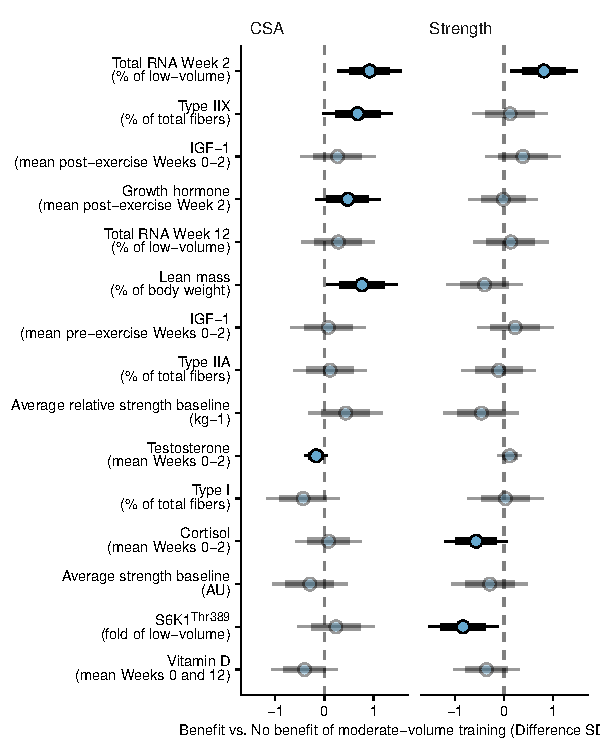
\includegraphics{thesis_files/figure-latex/univariate-benefit-analysis-1} 

}

\caption[Univariate analysis of potential determinants of benefit to moderat- over low-volume training]{Differences between groups classified as either having benefit or no benefit of moderate-volume training. For the sake of comparison, all variables have been scaled by their SD. Thick errorbars indicate a 80\% CI and thin errorbars indicate the 95\% CI. Transparent points and errorbars indicate that the variables was removed from further modeling. Sex was included as a covariate in all comparisons.}\label{fig:univariate-benefit-analysis}
\end{figure}
The choice of a dichotomized response variable (benefit vs.~no benefit) entailed the use of logistic regression. An assumption of this type of regression modeling is the linearity of the logit
(299).
As all variables did not meet this assumption when fitted in logistic regression, they were categorized into biologically meaningful categories (Vitamin D insufficient/sufficient), dichotomized based on measurement detection limits (testosterone in females), or sex-specific median values (lean body mass and testosterone in males).
A stepwise approach was used to remove variables that did not display association with the response variables. The process of stepwise removal of predictors are visualized in Figure \ref{fig:model-reduction-plot}.
Additional benefit of moderate- over low-volume training for changes in muscle cross sectional-area was predicted by individual differences between volume conditions in Total RNA at Week 2 and baseline lean body mass dichotomized to above or below the sex-specific median.
Only individual differences between volume conditions in Total RNA at Week 2 remained in the model after variable selection for muscle strength.
\begin{figure}

{\centering 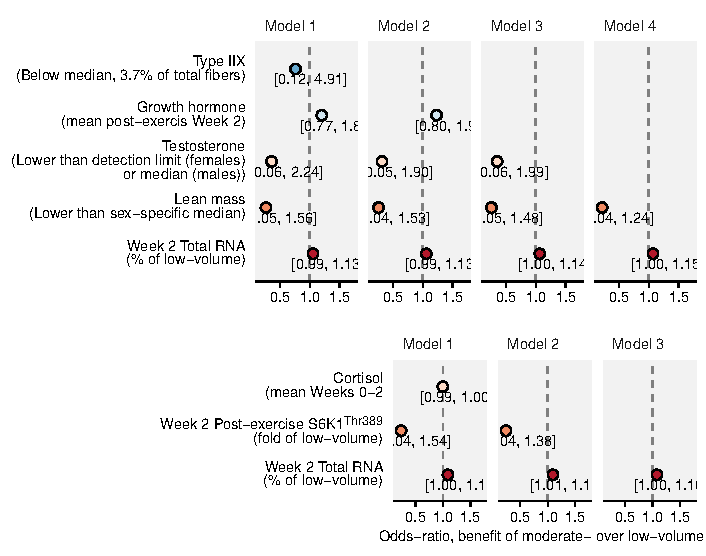
\includegraphics{thesis_files/figure-latex/model-reduction-plot-1} 

}

\caption[Step-wise variable selection of determinants of moderate- over low-volume training benefit.]{Sequential removal of predictors of moderate-volume benefit. Point estimates for each predictor are displayed with 95\% confidence intervals.}\label{fig:model-reduction-plot}
\end{figure}
The rationale for using dichotomized outcomes was, as mentioned above, to specifically explore determinants of \emph{individual} benefit of additional training volume, regardless of the magnitude of the difference between conditions.
This choice of analytic approach arose from discussions regarding clinical decision-making, where each individual's potential benefit should guide the choice of training methods.
Although linked to the specific study question, a dichotomized outcome variable could potentially mask other important associations in the data due to loss of information associated with the transformation
(320).
A primary hypothesis in the study was that the baseline muscle phenotype, specifically a ``glycolytic'' vs.~a ``aerobic'' phenotype (measured as high vs.~low type IIX content) would not show relative benefit of moderate-volume training.\footnote{\href{https://clinicaltrials.gov/ct2/show/NCT02179307?term=lillehammer\&draw=2\&rank=9}{As outlined in the Study's pre-registration}}
If such a marker would hold any prognostic value, it could potentially guide decisions regarding the training process.
In analysis, the phenotype marker measured as Type IIX counts was included together with other potential predictors of individual benefit of higher training-volume.
Both pre-training characteristics that could aid in clinical decision making and markers arising from the training itself were included in the analysis.
In order to select important determinants from this set of potential determinants, a stepwise procedure for variable selection, known as purposeful selection was used
(299).
Generally, stepwise variable selection has been criticized for a number of reasons, including arbitrarily searching for a single best model, over-estimation of regression parameters, and sensitivity to small changes in the investigated data set
(321, 320).

The question was slightly rephrased in a secondary analysis to address the limitations mentioned above, aiming to explore the association between potential determinants and individual differences between moderate- and low-volume training.
As shown in Figure \ref{fig:continuous-determinants}a, only Total RNA content at Week 2 in the moderate-volume leg, expressed as a percentage of the low-volume leg RNA content, positively associated with differences between volume conditions in muscle hypertrophy (CSA) and strength gains. These relationships are plotted in Figure \ref{fig:continuous-determinants}b.

Together with previous studies
(196, 198, 199),
as well as the direct correlation between RNA content and muscle hypertrophy presented earlier in this text
(Figure \ref{fig:rrna-csa-fig}),
the identification of volume-dependent total RNA regulation as a predictor of moderate-volume benefit in muscle mass and strength suggests an important role for early-phase ribosomal accumulation as a determining factor for muscle hypertrophy and strength.
Participants showing greater increases in ribosomal content in response to higher training volume at Week 2 also displayed greater relative benefit of the higher volume.
This likely acts through an increased translational capacity and confirms observations regarding volume-dependence in regulation of total RNA, mature rRNA species (rRNA 18S, 28S and 5.8S) and subsequent muscle hypertrophy (and strength gains).
\begin{figure}

{\centering 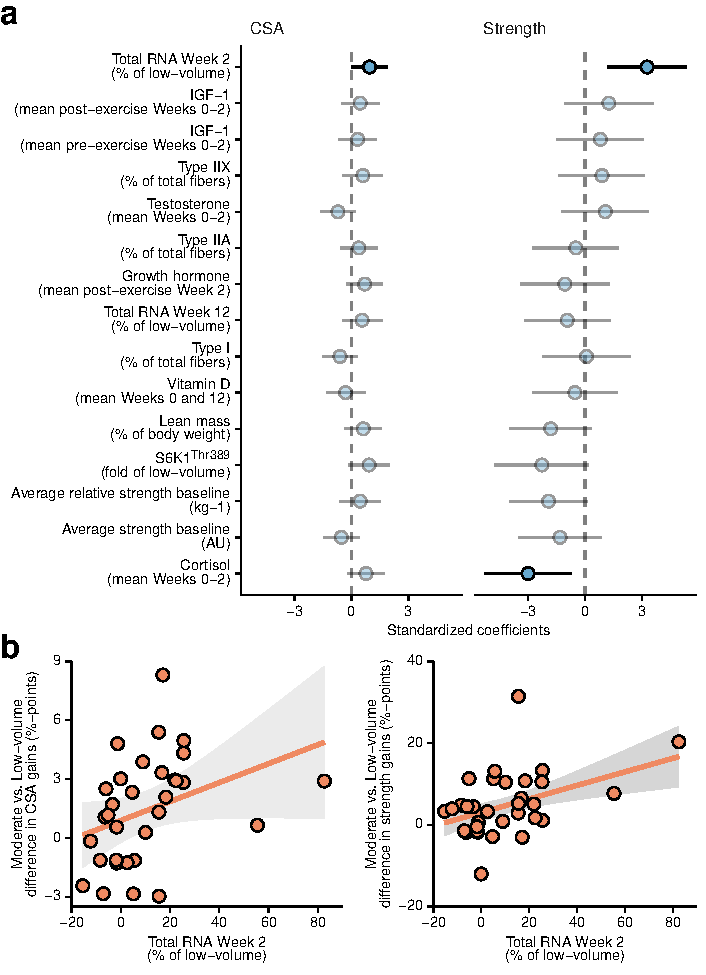
\includegraphics{thesis_files/figure-latex/continuous-determinants-1} 

}

\caption[Determinanats of moderate- over low-volume benefit]{Predictors of differences in outcomes between moderate- and low-volume training. Values in (a) are standardized regression coefficients with 95\% CI from univariate robust regression. Positive estimates indicate a positive association. Variables related to blood parameters, body composition and muscle strength was mean centered per sex.}\label{fig:continuous-determinants}
\end{figure}
In primary analyses, the percentage of lean body-mass was identified as a predictor of additional benefit of moderate-volume training for muscle hypertrophy.
Albeit associated with a large degree of uncertainty, this indication was in line with current prescription guidelines recommending greater training volume for experienced individuals
(17).
When analyzed between benefit categories, participants who displayed benefit of moderate- over low-volume training had a 4.3\%-point {[}0.3, 8.3{]} higher lean body mass than participants in the no benefit-group.
Lean body mass did not, however, display a linear relationship with individual differences between volume-conditions.
This, together with the fact that we did not find any robust relationship between pre-training Type IIX fiber proportions and differences in training outcomes between volume conditions, underlines that such markers have low prognostic value, even though they are readily adapted to the training regime as such.
This likely relates to the fact that traits such as fiber type, or body composition are genetically determined
(322, 94)
in addition to influenced by any history of physical activity.

In strength analyses, resting average cortisol levels sampled during the first two weeks showed a negative association with benefit of moderate- over low-volume training. This association was not found in muscle hypertrophy, indicating that factors other than muscle mass drove this relationship. Although speculative, higher levels of cortisol may be a response to the novelty of the training regime
(323).
Whether this translates in motor learning or other components of the neuromuscular response to different training volumes remains to be determined.

\hypertarget{predictors-of-additional-benefit-of-added-training-volume-meta-analysis}{%
\section{Predictors of additional benefit of added training volume: Meta-analysis}\label{predictors-of-additional-benefit-of-added-training-volume-meta-analysis}}

A meta-analysis was conducted to further explore potential factors associated with benefit of added training volume, interactions between study parameters such as age, sex, body-half, and weekly number of sets (previously reported without interactions in Figure \ref{fig:comb-fig-s1}).

The weekly number of sets did not interact with age, training status, or sex for either muscle mass or strength (interaction estimates are shown in Table \ref{tab:meta-interaction-table}), indicating that the literature currently gives little support for such demographic variables to guide prescription regarding training volume.

In contrast to what has been previously reported
(25),
the present analysis did not indicate any robust differences between unspecific (e.g.~DXA) or specific (e.g.~MRI or muscle thickness measured with ultrasound) muscle hypertrophy measures.
However, specific assessment of muscle strength, e.g., measures of one repetition maximum in exercises used in the training program, consistently showed larger positive effects of additional volume (Table \ref{tab:meta-interaction-table}).
Unspecific assessments of muscle strength were shown not to reflect additional training volume (effect size change per one weekly additional set 95\% CrI: {[}-0.027, 0.025{]}). This may indicate that specific motor learning is a factor influenced by training volume.

A consistent finding between muscle mass and strength measures was the negative effect seen in upper- compared to the lower-body measures.
These results suggest that adding a weekly set to upper-body programs will not robustly lead to increased strength measures (upper-body effect size change for every additional weekly set 0.003 {[}-0.014, 0.02{]}).
The effect of an additional weekly set in the upper-body for measures of muscle mass was still positive (0.011 {[}0.002, 0.021{]}) albeit lower when compared to the effect seen in the lower body (Table \ref{tab:meta-interaction-table}).
Together this indicates that muscles more active in every day activities will benefit to a greater extent by additional training volume, compared to upper-body muscles.
Studies examining volume-dependence in molecular determinants to resistance-training adaptations between different muscle groups are limited.
However, Hanssen \emph{et al.} found different satellite cell activation between volume-conditions in \emph{m. vastus lateralis} but not in \emph{m. trapezius}, coinciding with volume-dependence in outcomes in lower- but not upper-body muscles
(146,257).
Whether satellite cells \emph{per se} were responsible for this effect or if it represents a general inability of upper-body muscles to differentiate between two relatively strong stimuli remains to be explored.

The study's length interacted differently in muscle mass and strength models where more extended training periods seemed to reduce the positive effect of added training volume on muscle mass, albeit likely to a negligible degree. However, strength outcomes were positively influenced by the training period's length (Table \ref{tab:meta-interaction-table}). This may be an effect of different time courses in muscle mass and strength measures in response to resistance training.
\begin{table}

\caption{\label{tab:meta-interaction-table}Interaction between study parameter and weekly number of sets from meta-analyses on muscle mass and strength}
\centering
\fontsize{7}{9}\selectfont
\begin{tabular}[t]{lllll}
\toprule
\multicolumn{1}{c}{ } & \multicolumn{2}{c}{Muscle mass} & \multicolumn{2}{c}{Muscle strength} \\
\cmidrule(l{3pt}r{3pt}){2-3} \cmidrule(l{3pt}r{3pt}){4-5}
Interacting variable & Estimate & 95\% CrI & Estimate & 95\% CrI\\
\midrule
\addlinespace[0.3em]
\multicolumn{5}{l}{\textbf{Age}}\\
\hspace{1em}30-50 vs. 18-20 years & -0.011 & [-0.044, 0.02] & -0.037 & [-0.103, 0.028]\\
\hspace{1em}50- vs. 18-20 years & -0.004 & [-0.025, 0.016] & 0.005 & [-0.034, 0.044]\\
\hspace{1em}Mixed ages vs. 18-20 years & 0.005 & [-0.047, 0.055] & 0.005 & [-0.083, 0.092]\\
\addlinespace[0.3em]
\multicolumn{5}{l}{\textbf{Training status}}\\
\hspace{1em}Trained (> 1 year RT) vs. untrained & -0.001 & [-0.019, 0.016] & -0.025 & [-0.058, 0.007]\\
\addlinespace[0.3em]
\multicolumn{5}{l}{\textbf{Sex}}\\
\hspace{1em}Female vs. male & 0.001 & [-0.014, 0.015] & -0.012 & [-0.045, 0.018]\\
\hspace{1em}Mixed sex vs. male & -0.013 & [-0.038, 0.012] & 0.009 & [-0.044, 0.059]\\
\addlinespace[0.3em]
\multicolumn{5}{l}{\textbf{Body portion}}\\
\hspace{1em}Upper-body vs. lower-body & -0.005 & [-0.008, -0.002] & -0.029 & [-0.038, -0.02]\\
\hspace{1em}Whole-body vs. lower-body & -0.012 & [-0.034, 0.01] &  & \\
\addlinespace[0.3em]
\multicolumn{5}{l}{\textbf{Measurement technique}}\\
\hspace{1em}Unspecific vs. Specific estimation & -0.004 & [-0.01, 0.003] & -0.031 & [-0.06, -0.005]\\
\addlinespace[0.3em]
\multicolumn{5}{l}{\textbf{Length of study}}\\
\hspace{1em}Weeks & -0.001 & [-0.001, 0] & 0.005 & [0.003, 0.006]\\
\bottomrule
\end{tabular}
\end{table}
\hypertarget{characteristics-of-early-phase-training-induced-ribosome-biogenesis}{%
\section{Characteristics of early-phase training-induced ribosome biogenesis}\label{characteristics-of-early-phase-training-induced-ribosome-biogenesis}}

Study II aimed to further characterize early-phase total RNA accumulation in response to resistance training given its importance for subsequent adaptations, evident from analyses between- and within-participants.
By utilizing a mixed design, Study II assessed the effect of resistance training \emph{per se} when comparing a control group to a training group and variations in training volume in participants with different volume-protocols allocated to either leg (see figure \ref{fig:study2-overview} for an overview). The training protocol resulted in increased muscle mass, measured as \emph{m. vastus lateralis} muscle thickness, compared to the non-training control group (Figure \ref{fig:study2-muscle-strength-mass}a). This increase coincided with an increase in strength, most pronounced when measured as isokinetic torque (Figure \ref{fig:study2-muscle-strength-mass}b). The different training protocols (constant vs.~variable volume) were analyzed together concerning muscle mass and strength increases, as they led to similar changes.
These observations indicated the training program's efficacy in inducing changes to the neuro-muscular apparatus, specifically concerning muscle mass.
\begin{figure}

{\centering 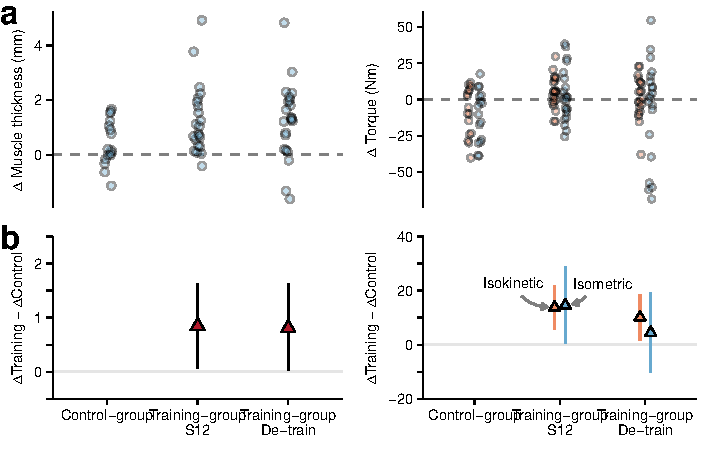
\includegraphics{thesis_files/figure-latex/study2-muscle-strength-mass-1} 

}

\caption[Muscle mass and strength changes in Study II]{Training induced changes in muscle mass (a) and strength (b) compared to non-training controls in Study II. Values in the training group are averaged over volume-conditions.}\label{fig:study2-muscle-strength-mass}
\end{figure}
Changes in muscle mass and strength were accompanied by a training-induced increase in total RNA per-unit-muscle weight. Compared to the control group, this was evident after twelve sessions (post-training, Figure \ref{fig:study2-rrna-vs-ctrl}a).
After the de-training period, total RNA decreased compared to after the twelfth session (-19.2\%, {[}-29.1, -8.1{]}), although still on average elevated compared to baseline, it was not robustly different to the control group (de-training in Figure \ref{fig:study2-rrna-vs-ctrl}a).
The initial session induced rRNA transcription as 45/47S pre-rRNA increased compared to non-training controls (Session 1, Figure \ref{fig:study2-rrna-vs-ctrl}b). This increase was still apparent after twelve sessions and then accompanied by greater mature rRNA levels (28S and 18S, Figure \ref{fig:study2-rrna-vs-ctrl}b). After the period of de-training, pre-rRNA levels returned towards levels seen in the control group, but mature transcripts were still elevated in the training group compared to controls, suggesting a decreased \emph{de novo} rRNA transcription (Post-training + de-training, Figure \ref{fig:study2-rrna-vs-ctrl}b).

Together with Study I and several others,
(324, 325, 203, 205,
196,198, 193, 162),
Study II confirms that resistance training leads to RNA accumulation, following an increased \emph{de novo} transcription and subsequent rRNA accumulation. After the eight-day de-training period, pre-rRNA levels' apparent normalization indicates that ribosomal biogenesis is coupled with up-stream stresses, such as resistance training. Such coupling is possibly due to the relative cellular expense associated with ribosomal biogenesis (207).
To further test the hypothesis that ribosome biogenesis would reflect reduced/increased training stress, training volume was manipulated in one leg and held constant in the other in participants recruited to the training group.
After four sessions performed with the same volume (six sets), the variable-volume leg trained four sessions with reduced volume (three sets) followed by four sessions with increased volume (nine sets). Small differences between volume conditions in 45S pre-rRNA levels at 48 hours after session twelve indicated that rRNA transcription was affected by the increased volume in the last block. However, this did not manifest in differences between volume conditions in total RNA or rRNA as they increased similarly in both conditions (Figure \ref{fig:study2-rrna-volume-conditions}a and b). Together this indicates that although ribosomal biogenesis to some degree is controlled in an on-demand manner, fluctuations in training volume over a relatively short period (\(\sim\) 1-2 weeks) after initial training performed with similar volume does not influence ribosomal accumulation to any meaningful extent.
However, it may also indicate that untrained individuals maximize rRNA transcription and RNA accumulation during initial sessions during a training program.
Indeed, the training-associated increase in total RNA abundance occurred primarily during the first part of the intervention. In sessions, one to four, total RNA increased by 8.6\% {[}5.5, 11.7{]} per session, followed by attenuated accumulation from sessions four to eight (1.9\% {[}-0.9, 4.7{]} increase per session) and eight to twelve (0.0\% {[}-3.1, 3.2{]} increase per session). This increase corresponded to increases from baseline to 48 hours after session four, eight, and twelve, respectively, of 38.9\% {[}23.9, 55.4{]}, 49.5\% {[}34.2, 66.5{]} and 49.5\% {[}32.5, 68.6{]}.
\begin{figure}

{\centering 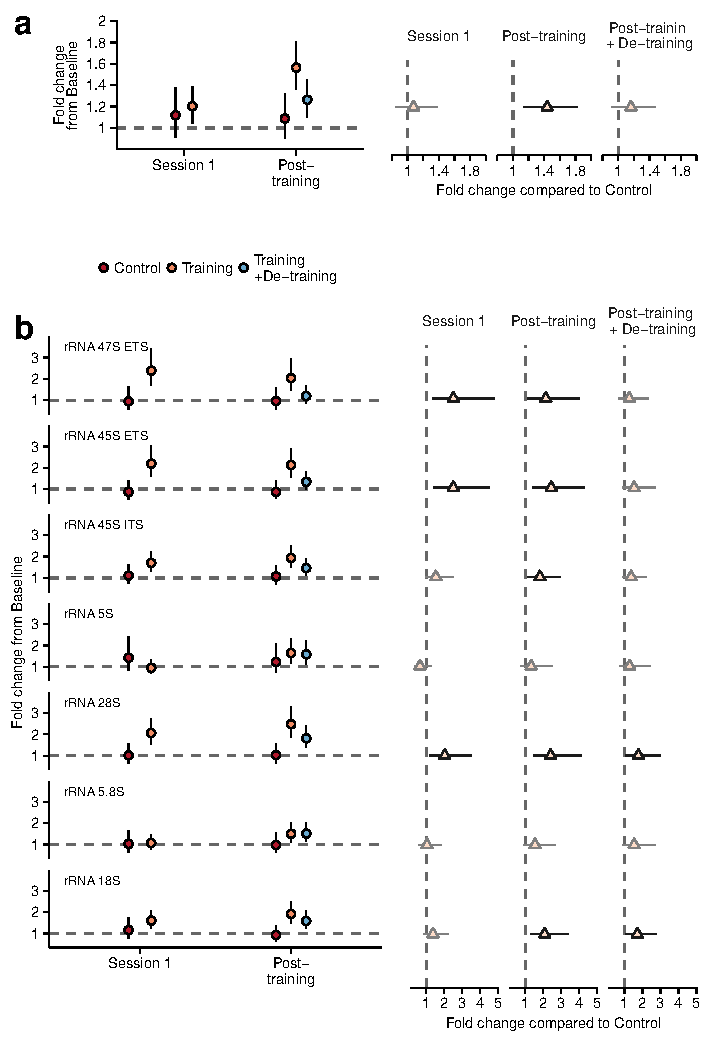
\includegraphics{thesis_files/figure-latex/study2-rrna-vs-ctrl-1} 

}

\caption[rRNA and total RNA changes in response to resistance training.]{Resistance training led to increased rRNA (a) and total RNA (b) abundance per tissue weight. Conditions in the experimental group are presented together.}\label{fig:study2-rrna-vs-ctrl}
\end{figure}
Although ribosomal biogenesis is a well-known characteristic of resistance training, its true time-course has been speculative.
Study II indicates that relatively few training sessions are needed to maximize total RNA per unit tissue weight.
Together with Study I and others that have performed repeated biopsy sampling (193), this suggests that young males and females will reach peak training-induced values within four to nine sessions, followed by a plateau.
Since the plateau phase occurred without a concomitant reduction in pre-rRNA levels, it may represent a dilution effect rather than decreased rRNA transcription. With increased muscle growth and cellular protein accretion, the ribosomal concentration is effectively balanced
(281)\\
Possibly, a progressive increase in training volume could abolish such a plateau-effect. Haun \emph{et al.} induced increases in total RNA throughout six weeks of training in well-trained participants, presumably by continuously increasing training volume (from 2-4 to 8-12 sets per exercise). This observation suggests that a progressive volume may increase ribosomal abundance to a higher degree than constant-volume protocols.
However, the lack of a relevant control condition warrants more research.
\begin{figure}

{\centering 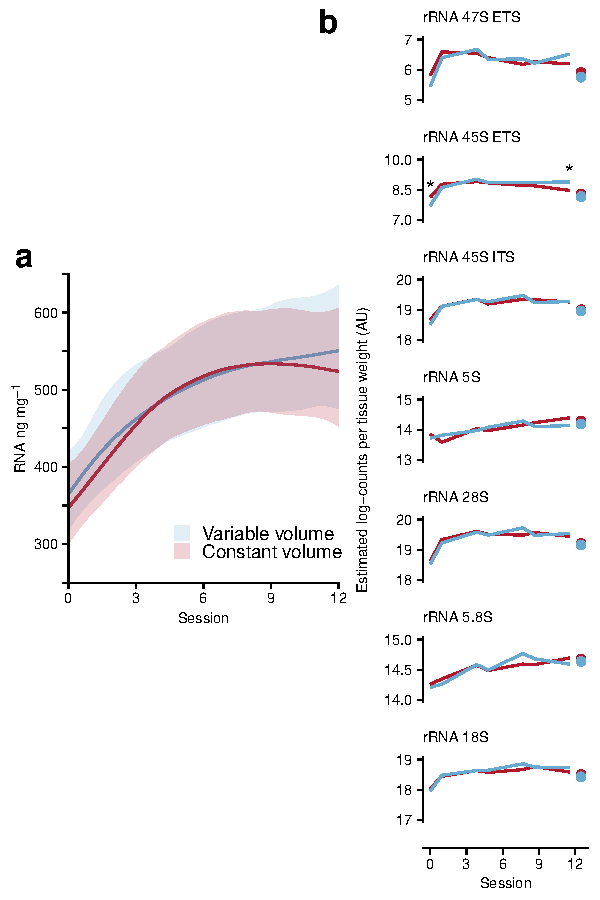
\includegraphics{thesis_files/figure-latex/study2-rrna-volume-conditions-1} 

}

\caption[Total RNA (a) and rRNA (b) abundance in response to resistance training in variable- and constant-volume training conditions. Asterisk indicate robust difference between volume conditions.]{Total RNA and rRNA abundance in response to training in Study II.}\label{fig:study2-rrna-volume-conditions}
\end{figure}
\begin{table}

\caption{\label{tab:ubf-rps6-regression-table}Effect of UBF and rpS6 levels, sessions and de-training on RNA-levels.}
\centering
\fontsize{7}{9}\selectfont
\begin{threeparttable}
\begin{tabular}[t]{lrrrr}
\toprule
\multicolumn{3}{c}{ } & \multicolumn{2}{c}{95\% CrI} \\
\cmidrule(l{3pt}r{3pt}){4-5}
Coefficient & Estimate & SD & Lower & Upper\\
\midrule
\addlinespace[0.3em]
\multicolumn{5}{l}{\textbf{UBF}}\\
\hspace{1em}Intercept & 5.91 & 0.06 & 5.80 & 6.03\\
\hspace{1em}UBF protein levels (SD-units) & 0.06 & 0.02 & 0.02 & 0.10\\
\hspace{1em}Session 1-4 & 0.08 & 0.01 & 0.05 & 0.10\\
\hspace{1em}Session 4-8 & -0.06 & 0.02 & -0.11 & -0.02\\
\hspace{1em}Session 8-12 & -0.02 & 0.03 & -0.07 & \vphantom{1}0.03\\
\hspace{1em}De-training & -0.19 & 0.07 & -0.32 & -0.06\\
\hspace{1em}Between Participant variation & 0.13 & 0.04 & 0.06 & 0.23\\
\hspace{1em}Between Participant:Leg variation & 0.03 & 0.03 & 0.00 & 0.10\\
\hspace{1em}Residual SD & 0.22 & 0.01 & 0.19 & 0.24\\
\addlinespace[0.3em]
\multicolumn{5}{l}{\textbf{rpS6}}\\
\hspace{1em}Intercept & 5.88 & 0.06 & 5.77 & 6.00\\
\hspace{1em}rpS6 protein levels (SD-units) & 0.01 & 0.03 & -0.04 & 0.07\\
\hspace{1em}Session 1-4 & 0.08 & 0.01 & 0.05 & 0.11\\
\hspace{1em}Session 4-8 & -0.06 & 0.03 & -0.11 & -0.01\\
\hspace{1em}Session 8-12 & -0.02 & 0.03 & -0.07 & 0.03\\
\hspace{1em}De-training & -0.21 & 0.07 & -0.34 & -0.07\\
\hspace{1em}Between Participant variation & 0.13 & 0.05 & 0.06 & 0.24\\
\hspace{1em}Between Participant:Leg variation & 0.03 & 0.02 & 0.00 & 0.09\\
\hspace{1em}Residual SD & 0.22 & 0.01 & 0.20 & 0.25\\
\bottomrule
\end{tabular}
\begin{tablenotes}[para]
\item The dependent variable is total RNA levels (log). Session 1-4 represents the slope in response to session 1-4 with Session 4-8 and 8-12 representing changes in slopes.
\end{tablenotes}
\end{threeparttable}
\end{table}
The general patterns seen in total RNA and mature rRNA in response to resistance training were also seen in ribosomal protein S6 (rpS6) and upstream binding factor (UBF) protein levels which both displayed increases after twelve training sessions, compared to non-training controls. After the de-training period, rpS6 levels were still elevated although not robustly greater than controls. However, UBF levels were measured above control levels
(Figure \ref{fig:study2-ubf-rps6-fig}a).
Together, this indicates general coordination between training-induced synthesis of rpS6 and rRNA transcription and a potential role of increased UBF levels in maintaining an increased rRNA transcription.
The associations between total RNA, rpS6, and UBF protein levels were analyzed to explore such coordination further. When controlling for time, UBF levels positively predicted RNA levels in the training group. For every unit increase in UBF (standard deviations), total RNA increased by 6.3\% {[}1.8, 11.0{]}. No such relationship was found between RNA levels and rpS6 (Table \ref{teb:ubf-rps6-regression-table}).
\begin{figure}

{\centering 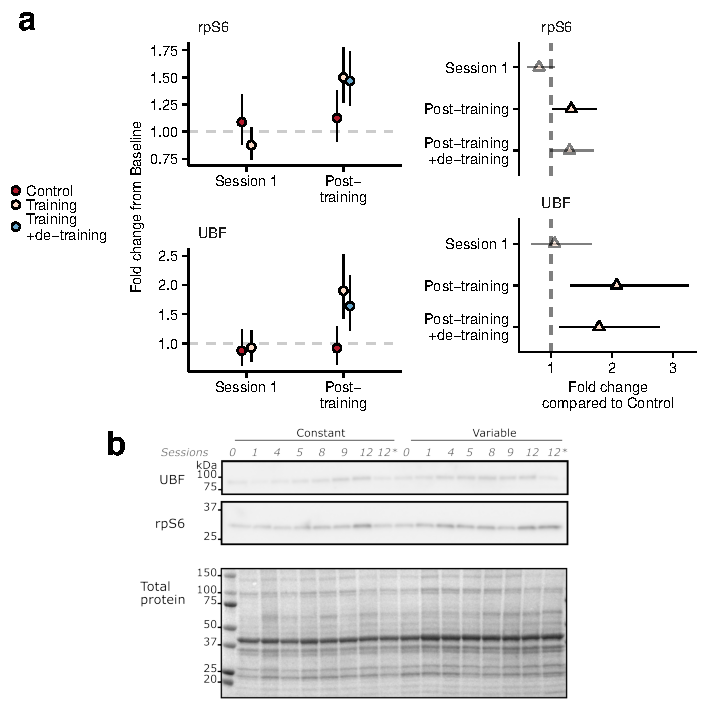
\includegraphics{thesis_files/figure-latex/study2-ubf-rps6-fig-1} 

}

\caption[UBF and rpS6 protein in resposne to resistance training in Study II.]{Ribosomal protein S6 (rpS6) upstream bindning factor (UBF) protein in response to resistance training in compared to non-training controls}\label{fig:study2-ubf-rps6-fig}
\end{figure}
Although resistance training led to a general increase in both rRNA and rpS6, the apparent disconnect in regression analyses suggests that regulation of rpS6 expression and ribosomal RNA transcription displays different temporal characteristics. Such disconnect may relate to different stability of ribosomal components or ribosomal proteins having extra-ribosomal functions affecting their expression
(326).\\
The relationship between UBF levels and total RNA underlines an essential role of UBF in ribosomal biogenesis. Mechanistically, UBF is needed for rRNA transcription, acting by recruiting secondary factors to the rDNA promoter and thereby enabling RNA Pol I controlled transcription
(210).
mTORC1 controls activation and availability of UBF as its inhibition blocks rRNA transcription
(212, 213).
In response to acute exercise, UBF activates through phosphorylation
(327, 198).
However, mechanical loading also leads to increased levels of total UBF, an effect shown to be insensitive to mTORC1 inhibition
(327,168, 198),
but instead mediated by increased c-Myc-induced UBF mRNA transcription (220).
In cell models, the availability of UBF \emph{per se} has been shown to regulate rRNA transcription
(214) by stimulating rDNA transcription
(215).
Together with observations made in Study II, this suggests that training-induced increases in UBF contribute to rRNA accumulation \emph{in vivo}.

\hypertarget{resistance-training-induced-increase-in-total-rna-predicts-muscle-growth}{%
\subsection{Resistance-training induced increase in total RNA predicts muscle growth}\label{resistance-training-induced-increase-in-total-rna-predicts-muscle-growth}}

As indicated in Study I, and previous studies, ribosome biogenesis is a determining process for resistance training-induced muscle growth
(198, 162,196,199),
To further explore this relationship, changes in total RNA abundance over the training period were estimated from each participant's leg (Figure \ref{fig:study2-rna-muscle-thickness}c) and used to model muscle growth measured as increases in \emph{m. vastus lateralis} thickness. There was a positive association between the magnitude of total RNA increase per session and muscle growth (Figure \ref{fig:study2-rna-muscle-thickness}a). This association was apparent when controlling for the average RNA abundance, expressed as the RNA level at Session 6 (estimated as the intercept-term in individual models). Conversely, when controlling for the increase in total RNA, total RNA abundance at Session 6 was negatively associated with muscle growth (Figure \ref{fig:study2-rna-muscle-thickness}b).
The association between total RNA increase and muscle growth was robust as no single measurement within-participant nor any single participant changed the conclusion from the analysis (Figure \ref{fig:study2-rna-muscle-thickness}d). Removing single observations or participants from the analysis did, however, lead to overlap between the 95\% CrI and the null-hypothesis (Figure \ref{fig:study2-rna-muscle-thickness}d).

This analysis supports the view of ribosomal biogenesis as an determining factor for resistance training-induced muscle growth
(198, 162,199,
196).
However, the analysis suggests that the increase \emph{per se} and not a fixed amount of total RNA, determines muscle growth.
A higher level of total RNA mid-training was instead associated with lowered muscle growth when controlling for the increase in RNA.
\begin{figure}

{\centering 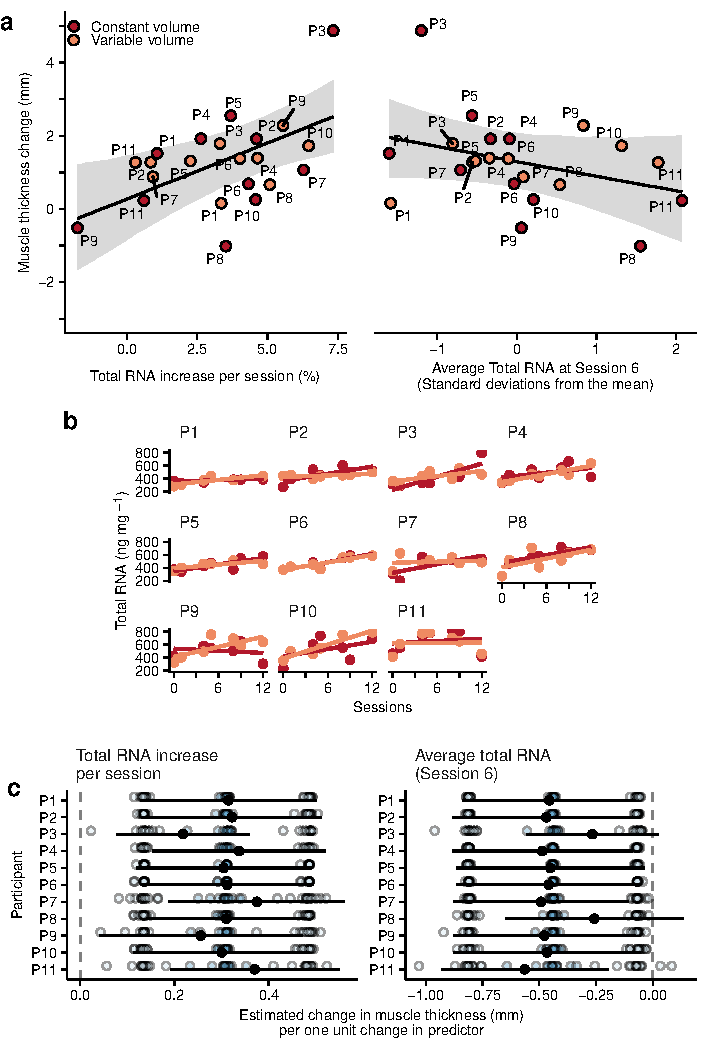
\includegraphics{thesis_files/figure-latex/study2-rna-muscle-thickness-1} 

}

\caption[Relationship between total RNA and muscle hypertrophy in Study II]{Muscle thickness increase predicted by total RNA increases and average total RNA abundance (a). Individual plots of estimates total RNA increases over time are shown in b together with results from leave-one-out analysis (c). Leave-one-out analysis shows the effect of removing a single participant (black point and error-bars) and individual values from the total RNA per time estimates where light-blue points represents bounds of the 95\% CI and blue points represents mean estimates.}\label{fig:study2-rna-muscle-thickness}
\end{figure}
\hypertarget{limitations}{%
\section{Limitations}\label{limitations}}

In Study I, a main objective was to determine differences in training outcomes and molecular markers between volume conditions. Therefore, the study is limited with respect to what conclusions can be drawn from time effects alone, as no non-training control group was included in the study. Conclusions regarding changes over time in, e.g., total RNA, gene expression, and strictly speaking, muscle growth and strength are limited in their strength of evidence.
In Study II, the use of a control group strengthens this aspect of the analyses. However, the number of biopsies was limited in the control group. The control group in Study II served the purpose of system validation but did not serve as a true control condition for training \emph{per se}.

In Study I, step-wise regression was used to select important variables relating to moderate-volume benefit. In addition to what was already discussed in previous sections, the analysis is limited concerning variables available for selection. Irrespective of the technique used for statistical analyses, the conclusion regarding the importance of total RNA is drawn when competing with the other available variables. From a cellular perspective, a plethora of potential determinants exists including, but not limited to,
satellite cells (221),
Yes-associated protein (328) and
Myostatin and transforming growth factor-\(\beta\) (329)
-related signaling. The availability of techniques in our lab to investigate these and other potential determinants limited analyses.
Additionally, the study did not include detailed documentation of out-of-study habitual physical activity, and only a limited dietary registration was performed, both of which could have influenced the between-participant analysis.
Lastly, by weighing variables against each other, one implicitly assumes that variables are measured with similar technical variability, which is likely a very optimistic assumption.

Ethical and practical reasons limit muscle biopsy sampling. In both studies, the choice of biopsy sampling time-points dictates the resolution of analyses. Biopsies sampled one hour after the fifth session in Study I likely did not provide reliable information regarding acute changes in gene expression in response to low- and moderate-volume exercise. Similarly, biopsies obtained at rest in Study II limited the investigation in terms of acute signaling events.

The use of total RNA as a proxy marker of ribosomal abundance is widely accepted
(281,330--332).
Indeed, we find general agreement between total RNA and targeted analysis of ribosomal RNA using qPCR, at least in the initial phase of the interventions. However, the apparent disconnect between mRNA and total-RNA pools and the tendency of discrepancies between volume conditions in total RNA and rRNA abundance after twelve weeks of training in Study I warrants further examination as it suggests that sub-populations of RNA may vary independently from each other. Although the assumption regarding total RNA likely holds in the initial phase of the programs examined, it should have been confirmed to strengthen conclusions from both studies.

\hypertarget{future-directions}{%
\section{Future directions}\label{future-directions}}

The importance of early-phase RNA accumulation was highlighted in both studies presented in this thesis. Future studies that aim to investigate \emph{in vivo} ribosomal biogenesis in response to resistance training should take advantage of the fact that a limited number of training sessions are needed to reach maximal accumulation of total RNA (and thus presumably ribosome abundance). Further use of within-participant designs could also investigate the etiology of inter-individual differences in ribosomal biogenesis. Constant-volume protocols may, in this respect, represent a fruitful model to investigate such differences. Given that training volume likely is the most important variable concerning resistance training dose-response, within-participant models with differentiated volume allocated to either limb could be used to study if, e.g., age-related anabolic resistance is related to impaired sensitivity to the training stimuli.

Although constant volume protocol may prove useful in controlled mechanistic studies, the use of progressive-volume protocols should be evaluated for their use in clinical settings. Ever since the days of DeLorme (see Background), progressive resistance training has been progressive with regard to absolute intensity. However, the use of a fixed training volume could be less effective as too much training volume initially may interfere with adaptations. Additionally, since there is little support for any diagnostic criteria for selecting initial training volume, evident from both Study I and the meta-analysis, progression of volume in short-term (1-3 months) training interventions could circumvent this issue.

\hypertarget{methodological-considerations}{%
\chapter{Methodological considerations}\label{methodological-considerations}}

This increased efficiency is due to the fact that between-participant variation can be removed from estimates of variability that in turn influence inference.
The contralateral model can be extended by utilizing a mixed design where additional conditions are allocated to participants\\
--\textgreater{}

\hypertarget{reliability-of-micro-biopsy-sampling}{%
\section{Reliability of micro-biopsy sampling}\label{reliability-of-micro-biopsy-sampling}}

The micro biopsy technique used in works presented in this thesis generally produces smaller samples than other biopsy techniques (333), and thus
requires several passes to produce sufficient material for multiple
downstream experiments. However, reports confirms that the micro-biopsy
technique is comparable to the traditionally used Bergström technique in
several measures of muscle characteristics at the same time as being
well-tolerated (260,334).
Any reported differences in fiber type distributions between sampling techniques have been suggested to be related to differences in sampling depth (334,335).
Thus, any biopsy technique's reproducibility may relate to its ability to obtain sufficient material at similar depths between samples.

In Study I, one or several pieces of muscle (total weight
\(\sim\)\SI{15}{mg}) were chosen per sampling for analysis of fiber type
composition. The average total number of counted fibers per sample was 539.
Only a small percentage (5.4\%) of samples did not contain enough fibers for representative analysis of fiber type composition (\textgreater{} 200 fibers),
(336)
and as many as 1400 fibers were counted in some specimens (\ref{fig:fiber-methods-fig}a).
The smaller amount of tissue obtained using the micro-biopsy technique did not limit fiber type composition analyses.

In order to assess the reproducibility of the technique, samples obtained during the same day (separated by \(\sim\) 2 hours) were analyzed as duplicate samples.
Similar to Blomstrand \emph{et al.} (336), standard deviations from duplicate measures were calculated as

\[SD = \sqrt{\frac{\sum{d^2}}{2n}}\]

Where \(d\) is the difference between paired observations and \(n\) is the number of pairs.
The variation (SD) between duplicate samples were 5.86 and 5.49 for Type I and IIA fibers, respectively (\ref{fig:fiber-methods-fig}b).
This did only marginally differ from between leg variations (Type I, 6.31; Type IIA, 6.24; Figure \ref{fig:fiber-methods-fig}c).
These estimates are slightly lower than those reported by Blomstrand \emph{et al.}, using the Bergström needle
(336). This suggests that the micro-biopsy technique is reproducible in terms fiber type composition.
\begin{figure}

{\centering 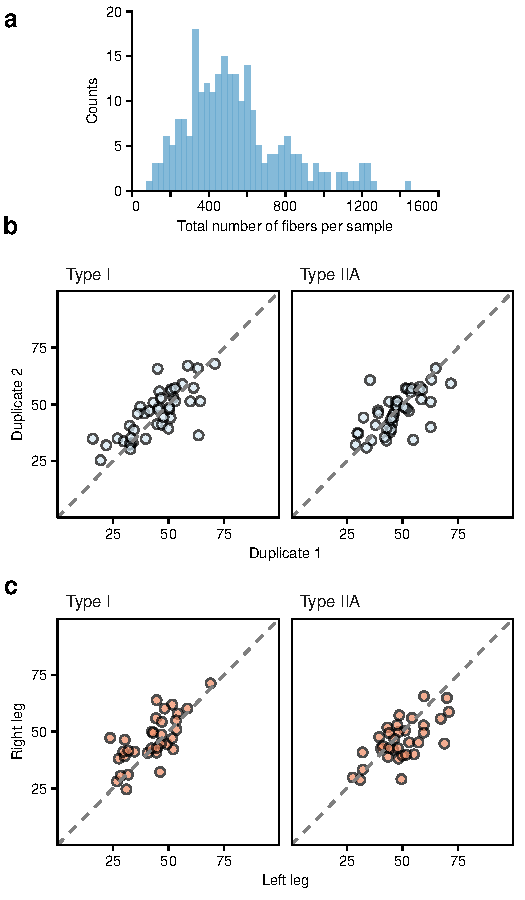
\includegraphics{thesis_files/figure-latex/fiber-methods-fig-1} 

}

\caption[Characteristics of biopsy samples used in immunohistochemistry analyses.]{Number of fibres in immunohistochemistry analyses (a), correlation between duplicate samples from the same leg (separated by 2 hours) (b) and correlations between samples from left and right leg pre-intervention.}\label{fig:fiber-methods-fig}
\end{figure}
\hypertarget{model-based-normalization-of-qpcr-data}{%
\section{Model-based normalization of qPCR data}\label{model-based-normalization-of-qpcr-data}}

Quantitative reverse-transcription real-time polymerase chain-reaction (qPCR) is the method of choice for conducting targeted gene-expression studies.
After reverse-transcription of RNA, complementary DNA (cDNA) is amplified in the presence of target-specific primers and a reporter probe or dye that produces fluorescence as the PCR product accumulates over repeated PCR cycles. When enough product has formed, the fluorescent signal rises above background fluorescence, and the fractional PCR cycle used for quantification (Cq) can be estimated. The Cq-values is directly proportional to the starting amount of the targeted transcript and thus constitute the primary outcome of qPCR experiments
(337).
qPCR experiments should ideally be designed to account for methodological pitfalls, including amounts of RNA utilized for reverse-transcription, its efficiency, and the amount of cDNA used in PCR amplification.
As traditional statistical treatment of qPCR data accounts for these challenges through the use of a reference-gene (338,339), the stable expression of such a gene is an important assumption in the experiment.
Using an internal control-factor comprised of the geometric average of multiple reference-genes has been shown to increase this assumption's validity (340).
However, the stability of potential reference genes must be determined in each experiment (340,341), highlighting that qPCR is inevitably challenging, specific to the system under study.
This challenge may be why many recent investigations into human skeletal muscle in response to exercise reported using a single-reference gene, validated or non-validated for normalization, despite the recommended use of a validated set of reference genes (342--346).

Several methods have been proposed to select a suitable set of references genes, out of which geNorm (340) and Normfinder (347) are the two most common approaches.
The geNorm algorithm assesses reference-gene stability through an iterative calculation of pairwise expression-ratios where the least stable gene, i.e., the gene that varies the most relative to other genes across all samples, is removed in each iteration, resulting in a set of at least two genes that exhibit the least pairwise variation (340).
As no information about the study design can be incorporated in geNorm, a potential pitfall is a variable expression of potential reference genes across experimental groups or conditions (347).
The Normfinder algorithm utilizes a linear model to determine variation in reference-gene expression as deviations from an assumed stable expression.
Normfinder can include a grouping factor, resulting in a stability measure that combines variation within and between groups for each gene.
This inclusion does not, however, relax the assumption of no \emph{systematic} variation across experimental conditions (347).

As many experiments performed in exercise-physiology, especially related to muscle, are conducted as repeated measurement studies, where the same participants are investigated over time, the question regarding reference-gene stability may be slightly rephrased. Instead of searching for the most stable gene across the whole data set, we may want to assess a set of genes' stability within each participant.
Dai and co-workers (348) suggested the utilization of a mixed-effects model-based selection algorithm.
First, the algorithm determines whether variation in expression of a potential set of reference-genes depends on experimental conditions.
Then, it determines the expression stability of gene-sets through the intra-class correlation within data clusters, e.g., study participants, where gene expression is to be monitored over repeated measures.
Such a mixed-effect model approach accounts for and takes advantage of correlated measures.
The proposed algorithm can also capture complex experimental designs and confirm that potential genes are not systematically affected by conditions studied.

To assess the stability of potential reference genes in Study I, 11 genes were evaluated (Figure \ref{fig:ref-gene-comp}a). All three selection algorithms suggested different reference genes (Figure \ref{fig:ref-gene-comp}b). The mixed-model approach resulted in a set of genes that showed the least systematic variation across study conditions. Figure \ref{fig:ref-gene-comp}c shows coefficients with 95\% CI from mixed models with each normalization factor as the dependent variable. The naive use of a single reference-gene would result in the largest deviation from the assumption of a stable reference over time, as GAPDH is expressed to a lesser degree before exercise at Week 2 compared to baseline. However, when comparing between conditions, normalization factors suggested by geNorm and Normfinder both showed differentiated levels between conditions before exercise at Week 2 (Figure \ref{fig:ref-gene-comp}c). These results underline that bias can be introduced in qPCR experiments from the choice of normalization factor. The use of a selection algorithm that tests explicitly for stability within participants may provide a more robust normalization factor.
\begin{figure}

{\centering 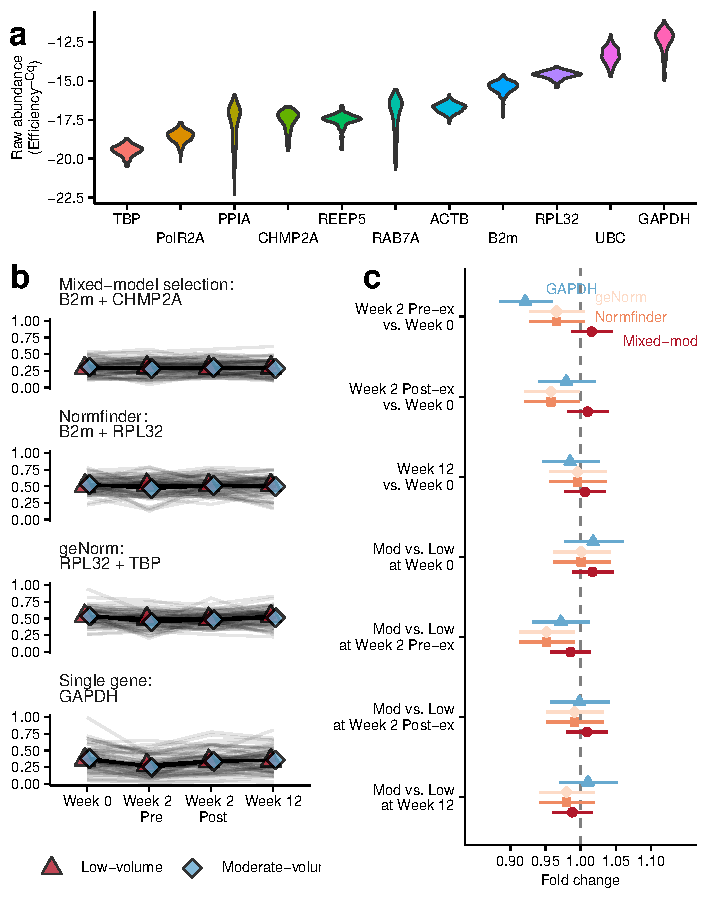
\includegraphics{thesis_files/figure-latex/ref-gene-comp-1} 

}

\caption[Reference gene selection in Study I]{Variation in normaliation factors determined by mixed-model selection, Normfinder and geNorm as well as comprised of a single-gene (GAPDH) for comparison (a). Estimates from mixed-effects regression-models for each normalization factor (b). Errorbars represent 95\% confidence intervals.}\label{fig:ref-gene-comp}
\end{figure}
The interpretation of qPCR data indirectly relates to the choice of biological input. When, e.g., total RNA is extracted and normalized per sample before cDNA synthesis, stable reference genes are assumed to be stable per total RNA. This logic also applies when a fixed amount of tissue or mRNA is used as an input quantity
(349).
Internal reference genes will if they are validated, thus reflect the input quantity. The interpretation in such a case is that target gene abundance changes per amount of biological input, e.g., total RNA.
As such, the validation of a set of reference genes may be redundant as normalization is performed when an equal amount of RNA is subjected to cDNA synthesis.
Additionally, reference genes are also measured with technical error and biological variation that is inevitably introduced to the analysis.
Modifications to the design of the qPCR experiment were suggested by Steibel and co-workers (350), who utilized a linear mixed-effects model framework where the model was specified with a random-effects structure designed to capture variations due to e.g.~sample preparation as well as the overall study design (though fixed-effects).
Technical variation was modeled as random effects of two or more technical replicates.
In this approach, all target genes are modeled together as a set, and the effect of experimental conditions are evaluated from the model for each gene-of-interest.
When utilizing a linear mixed-effects model, as suggested by Steibel \emph{et al.} (350), assumptions are made that errors are normally distributed, and variance is equal over the range of the data (homoscedasticity).
This assumption can be problematic when dealing with low-abundance genes as the variation increases when few target molecules are amplified (269).
Such model assumptions can be checked and delt with using appropriate statistical methods allowing for heterogeneous variance (270).
Further extending the concept described by Steibel \emph{et al.} (350), Matz and co-workers proposed modeling transcript abundance with a Poisson-lognormal generalized linear mixed-model (269). This model enables one to account for the specific characteristics of qPCR data, including no amplification (zero target molecules) and heteroscedasticity, i.e., larger variance due to low-abundance starting material.
Matz \emph{et al.} also suggested that the random-effects structure would provide sufficient within-model normalization (269).

As suggested by Steibel \emph{et al.} and Matz \emph{et al.}, the use of model-based normalization represents a promising alternative in situations where the appropriate validation of reference genes is not feasible.
However, the implementation of such analysis comes with a new set of assumptions.
First, if a study condition systematically leads to lower amounts or quality of cDNA due to, e.g., RNA degradation, a random effect structure will not account for this but instead result in estimates of lower expression of all genes in these samples. In such case, the use of internal reference genes will yield different results as the internal control will also be affected by RNA degradation
(269).
This fact leads to the assumption in a model-based normalization strategy that variations in cDNA quantity or quality between samples are randomly distributed.
Additional assumptions revolve around the choice of statistical model.
In the basic parameterization of a linear mixed-effects model, homoscedasticity and normal distribution of the residual errors are assumed.
As differently expressed genes can be assumed to have different overall variances, this would violate the assumption of homoscedasticity. To account for possible heterogeneity among different genes, a variance function
(270)
can be introduced to the model to allow for gene-specific residual variance. This approach can be extended with variance functions that also account for higher variation due to the stochastic processes when amplifying small amounts of starting material.
Such gene-specific residual variance can be modeled taking the observed Ct-value into account.
Adding variance-functions to the model could be regarded as an analog to the use of a Poisson log-normal model to account for qPCR specific technical variability, as suggested by Matz \emph{et al.}(269).

Implementations of model-based normalization can be accomplished both in a frequentist and Bayesian framework.
The \texttt{nlme} package provides functions to fit linear mixed-effects models (LMM) with extended variance structures that can account for gene-specific residual variance (270).
Matz \emph{et al.} (269) used the \texttt{MCMCglmm} (271) package to fit Bayesian generalized linear mixed models (GLMM) using a Poisson log-normal errors.

The introduction of more elaborate random effect-structures and variance structures adds parameters to each model that has to be estimated. This complexity may lead to convergence issues in linear mixed-effects models
(351).
Analogous to this, in a Bayesian framework, Markov chain Monte Carlo (MCMC) sampling may struggle to converge when models are too complex.
The robustness of modeling algorithms may thus represent a limitation in terms of reproducibility of model-based normalization.
To assess the robustness of model-based normalization strategies, all possible gene combinations of sizes 2 and 11 (both n = 78) from a set of 13 genes investigated in Study I were used to fit models using LMM and GLMM approaches.
The same random effect structure was used in both frameworks.
The fraction of models that did not converge (LMM) or showed estimation issues (LMM and GLMM) was determined for both modeling strategies. In the LMM approach, non-estimable effects were defined when the algorithm could not approximate the covariance matrix. In the GLMM approach, a Gelman-Rubin convergence criterion \textgreater{} 1.1 from two chains for any estimate was used as a threshold to define estimation issues.
The analysis showed that the number of models with convergence issues increased as the number of targets increased from two to eleven \ref{fig:qpcr-model-robustness}. To circumvent such convergence issues, simplification of random effect-structures or reducing the number of targets may help LMM and GLMM. Adding MCMC iterations in the Bayesian framework could improve its performance.
\begin{figure}

{\centering 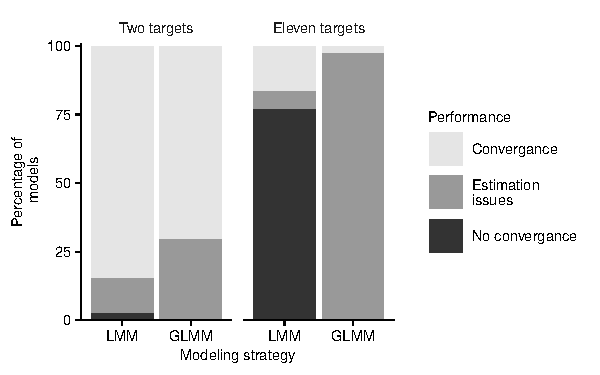
\includegraphics{thesis_files/figure-latex/qpcr-model-robustness-1} 

}

\caption[Robustness of model-based qPCR normalization]{Increasing the number of targets in gene-set modeling increses the rates of non-convergance and estimation issues in LMM as wells as estimation issues in GLMM. Estimation issues in LMM was defined when variance components were not estimatable, in the GLMM approach the Gelman-Rubin criterion was used to define estimation issues.}\label{fig:qpcr-model-robustness}
\end{figure}
The choice of a model-based normalization approach for qPCR analysis could also be based on statistical efficiency. As measurements of reference genes are associated with technical error and biological variation, relying on these measurements affects subsequent statistical tests' power. To explore the effect of model-based vs.~reference-gene based normalization on statistical power, a small simulation study was performed.
First, a simulated data-set of Ct-values for n = 1000 participants and four genes was created, designed to mimic the observed data-set in Study I. Random effects, common to all genes were added trough random sampling from distributions with zero mean and given standard deviations for participants (\(\sigma = 0.3\)), participants legs (\(\sigma = 0.001\)) and biological samples within-participant (\(\sigma = 0.27\)). Gene-specific random effects for each participant (\(\sigma = 0.25\)), leg (\(\sigma = 0.0001\)) and biological sample (\(\sigma = 0.1\)) were added. Gene-specific residual error was then added to each replicate where the sampling distributions were set to \(\sigma=0.2\) and \(\sigma=0.6\) in the genes-of-interest and \(\sigma=0.01\) and \(\sigma=1\) in the ``stable'' and ``unstable'' reference gene respectively. To further mimic the behavior of qPCR data, an additional random error was added where the sampling distribution had a standard deviation of \(\sigma = 0.2 \times Ct-min(Ct)\), which gave heteroscedasticity within each gene related to the simulated Ct. Together these parameters simulate the randomness of a qPCR data set with gene-specific heteroscedasticity over the range of simulated Ct-values with increased error in genes that were simulated as less abundantly expressed (higher Ct-values).
All genes where given the same average Ct-value of 20 and two genes where considered genes of interest where fixed-effects of time and interaction effects between time and condition were added representing fold-changes of \textasciitilde1.15-1.52 (differences in Ct-values of 0.2-0.6). Participants (n = 30) were randomly sampled from the simulated population and gene expression values were assessed either in model-based normalization approaches or a gene-by-gene manner where a single target was normalized to a reference gene and modeled using the same fixed effect structure as in the model-based approach.

The model-based normalization approaches were comparable and consistently better performing than the gene-by-gene strategy wherein target genes were normalized by reference-genes (Figure \ref{fig:qpcr-simulations}). Adding random variation to the target gene moved the model-based approach closer to the reference-gene normalization strategy (comparing \(\sigma=0.2\) with \(\sigma=0.6\)). On the other hand, adding random variation to the reference-gene naturally decreased statistical power compared to the stable versus the unstable reference gene.

In summary, the choice of analytic methods is potentially a source of significant variation in analyses of qPCR data and subsequent inference.
These notes underline that establishing and critically evaluating data-analytic pipelines adapted to specific experimental designs can explicitly test assumptions about both biological, technical, and statistical aspects of qPCR analysis.
Although using a model-based normalization approach could prove problematic in terms of model fitting, it is likely more accurate and powerful.
\begin{figure}

{\centering 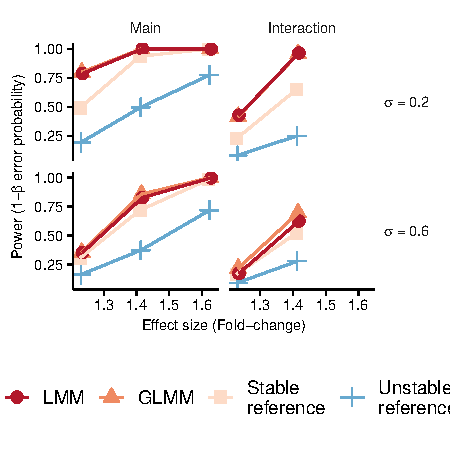
\includegraphics{thesis_files/figure-latex/qpcr-simulations-1} 

}

\caption[qPCR power-simulation]{Statistical power increases with effect-size. Effect sizes were assessed as main effects of time (left panels) or as interaction between time and group (right panels). Gene-specific variation in each target gene was set to $\sigma=0.2$ (upper panels) and $\sigma=0.6$ (lower panels).}\label{fig:qpcr-simulations}
\end{figure}
\hypertarget{increased-relevance-of-rna-seq-data-through-data-driven-selection-of}{%
\section{Increased relevance of RNA-seq data through data-driven selection of}\label{increased-relevance-of-rna-seq-data-through-data-driven-selection-of}}

Analysis of high-dimensional data such as those retrieved from RNA sequencing experiments requires the use of a multitude of bioinformatic and statistical tools. Such tools are continuously being developed and optimized for different tasks. This continuing development requires that a combination of tools are validated for specific study conditions (248)
To improve the interpretability of the RNA sequencing data obtained from Study I, we sought to compare mapping tools for their validity. As a first step, we utilized myosin heavy-chain compositions determined by immunohistochemistry to relate mRNA counts to protein levels. Myosin heavy-chains are well suited for this purpose as their mRNA and protein levels are known to correlate
(352, 100, 353).
To avoid concerns regarding normalization assumptions, both mRNA and protein abundances were expressed relative to the sum of counts for the whole gene- and protein-family
(354, 100).
This analysis indicated that transcript-based mapping tools
(RSEM (276),
kallisto (278) and Salmon (279))
resulted in stronger correlations between mRNA and protein profiles than genome-based mapping tools
(STAR (275)
and HISAT2 (274); Figure \ref{fig:rna-seq-myhc-validation}).
A second analysis utilized the within-participant design of the study. With the assumption that paired observations between legs, before the intervention would result in similar expression profiles if read mappings were more accurate, we determined the pairwise Log\textsubscript{2}-differences of a set of genes with known robust expression across tissues (355).
Across the whole range of transcript abundances (Average Log\textsubscript{2}-count), RSEM displayed smaller differences between pairwise observations, indicating less technical variation. RSEM differed marginally from other transcript-based tools but to a larger degree to genome-based tools (Figure \ref{fig:rna-seq-pairwise-validation}).

Mapping tools were used with default settings which leaves room for further optimization of each tool. However, selecting tools with default settings should provide a heuristic solution to the problem of optimizing an analytic pipeline. Taken together, these observations highlight that RNA sequencing experiments can be improved in terms of biological validity by systematic evaluation of analytic tools.
\begin{figure}

{\centering 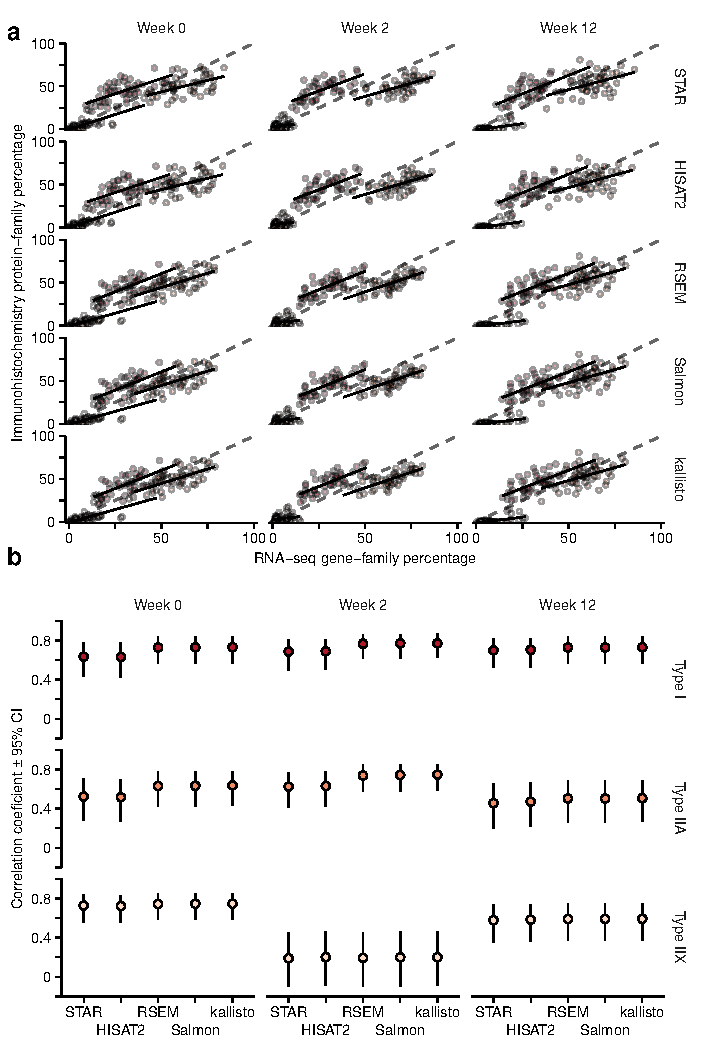
\includegraphics{thesis_files/figure-latex/rna-seq-myhc-validation-1} 

}

\caption[Correlations between gene-family normalized protein and gene data from different mRNA quantification methods.]{Validation of mapping tools using mRNA to protein correlations of myosin heavy-chain genes}\label{fig:rna-seq-myhc-validation}
\end{figure}
\begin{figure}

{\centering 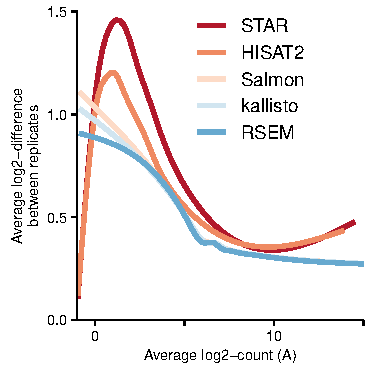
\includegraphics{thesis_files/figure-latex/rna-seq-pairwise-validation-1} 

}

\caption[Within-participant variation between RNA sequencing mapping tools.]{Average log-differences across average abundance levels for different mapping tools from paired samples retrieved prior to the intervention in Study I. Less difference indicate lower technical variation, assuming similarities between legs.}\label{fig:rna-seq-pairwise-validation}
\end{figure}
\hypertarget{conclusions}{%
\chapter{Conclusions}\label{conclusions}}

The main conclusions drawn from the work presented in this thesis are
\begin{itemize}
  \item muscle mass and strength are differentially affected by resistance training volume, expressed as the within-sessions number of sets, in a dose-dependent manner.
  \item Moderate compared to low-volume training leads to greater ribosomal biogenesis and mRNA expression related to extracellular matrix remodeling.
  \item Moderate compared to low-volume exercise leads to a higher activity of
mTORC1-related signaling.
  \item Resistance training-induced shifts in fiber type distributions are sensitive to training volume as moderate compared to low training volumes leads to a greater reduction in Type IIX proportions over twelve weeks of training but less reduction in response to four sessions.
  \item The ability to differentiate total RNA accumulation in response to different training volumes after four training sessions predicts benefits of moderate compared to low-volume training after twelve weeks.
  \item Maximal accumulation of total RNA in response to resistance training occurs after eight sessions in previously untrained young individuals.
  \item Accumulation of total and ribosomal RNA is not affected by variable training volume. However, eight days of de-training training reduced the synthesis of ribosomal precursor RNA and total RNA content.
  \item Total RNA abundance is positively related to upstream binding factor protein-expression.
\end{itemize}
\hypertarget{svensk-sammanfattning}{%
\chapter{Svensk sammanfattning}\label{svensk-sammanfattning}}

Systematisk styrketräning leder till en större skelettmuskelmassa och förbättrade funktionella egenskaper hos det neuromuskulära systemet. Dessa förändringar leder till generella hälsofördelar oavsett ålder och tidigare aktivitetsnivå. Genom att variera intensitet, val av träningsövningar och volym kan styrketräning skräddarsys för att anpassas till individuella mål och utgångspunkter. På vilka indikationer sådana förändringar av träningsbelastningar ska utföras är inte klart. Styrketräningens volym, uttryckt som antal serier per muskelgrupp och träningspass eller träningsvecka har identifierats som en viktig faktor för träningsresultaten. Det är dock sannolikt att individer varierar med avseende på volymberoende i träningsresultat som muskelmassa och styrka.

Det primära syftet med denna avhandling var att relatera anpassningar till styrketräning, genomfört med låg och måttlig volym till individuella egenskaper hos otränade individer.
Vidare syftade arbetet som presenteras här till att karakterisera hur träningsvolym påverkar molekylära
egenskaper i skelettmuskel och beskriva tidsförloppet för nybildning av ribosomer under den tidiga fasen av ett styrketräningsprogram.

I en första studie (Studie I) genomförde unga, friska, otränade manliga och kvinnliga deltagare (n = 34) en 12 veckor lång träningsintervention med 2-3 träningspass per vecka. Träningen genomfördes med en kontra-lateral träningsmodell där ett ben tränade med låg volym (en serie per övning) och det andra benet tränade med moderat volym (tre serier per övning).
Den främre lårmuskelns tvärsnittsarea och styrka mättes före och efter träningsperioden.
Muskelprover togs från den m. vastus lateralis före och efter träningsinterventionen samt före och en timme efter det femte träningspasset.

Träningsperioden ledde till muskelhypertrofi och ökad muskelstyrka, denna ökning var volymberoende med större framgångar som svar på moderat träningsvolym. Detta sammanföll med större aktivering av molekylär signalering och högre nivåer av markörer relaterade till nybildning av ribosomer. Vidare ledde träning med moderat volym till mer utbredd övergång från muskelfibertyp IIX till IIA. Tillsammans visade detta att moderat träningsvolym ledde till mer uttalade funktionella och biologiska anpassningar än träning med låg volym.
Tretton respektive sexton deltagare identifierades ha fördel av att träna med moderat träningsvolym då dessa fick större framgång med denna metod jämfört med låg träningsvolym. Dessa individer visade sig också ha en större ackumulering av RNA i benet som tränade med den högre träningsvolymen efter fyra träningspass. Detta indikerar att förmågan att differentiera nybildning av ribosomer i den inledande fasen av en träningsperiod förutsäger långsiktiga fördelar med moderat träningsvolym.

Resultaten från studie I kombinerades med tidigare studier i en metaanalys. Denna gav stöd för att träningsvolymen generellt sett är en viktig variabel då både muskelmassa och styrka ökar mer när träning genomförs med större volym. Meta-analysen visade dock att en ökad träningsvolym inte leder till ökad muskelmassa eller styrka i överkroppen.

RNA från ett urval (n = 25) av deltagarna i Studie I användes till RNA sekvensering. Urvalet gjordes baserat på RNA-kvalité. För att etablera en ändamålsenlig analys genomfördes en systematisk utvärdering av olika bioinformatiska verktyg. Dessa utvärderades bland annat baserat på variationen inom varje forskningsdeltagare innan träning inleddes och korrelationen mellan relativa nivåer av mRNA och protein av myosin (myosin heavy-chain).
Vidare användes olika normaliseringsstrategier för att kunna jämföra de olika träningsvolymerna. Detta då volymberoende ackumulering av RNA som svar på styrketräningen ledde till att olika mängder muskelvävnad användes i analyser då en bestämd mängd RNA användes vid förberedelse av analyserna.
Analyserna visade ett ökat uttryck av gener som var relaterade till den extracellulära stödstrukturen efter två veckors träning. Inga skillnader i genuttryck identifierades efter träningsperioden när hänsyn togs till den mängd musklevävnad som användes i vid förberedelse av analyserna. Detta i motsats till resultat från normaliseringsstrategier som inte tog samma hänsyn. Här identifierades istället kontraintuitivt högre uttryck av olika gener som svar på träning med låg volym.

Givet att nybildningen av ribosomer i inledningsfasen av en träningsperiod spelar en viktig roll för de långsiktiga träningsresultaten så genonfördes ytterligare en studie med syfte att vidare undersöka denna process. Specifikt ville vi beskriva tidsförloppet för träningsinducerad ackumulering av ribosomala markörer. Vidare ville vi undersöka om variationer i träningsvolym eller ett kortare träningsavbrott skulle påverka markörer för ribosomal nybildning.

Arton deltagare deltog i studien och ingick antingen i en träningsgrupp (n = 11) eller en kontrollgrupp (n = 7). Träningsgruppen genomförde tolv träningspass där det ena benet tränade lårets framsida med en konstant volym genom hela perioden (6 serier) och det andra benet tränade med variabel volym (6, 3 och 9 serier i träningspass 1-4, 5-8 och 9-12). Muskelbiopsier togs från m. vastus lateralis i träningsgruppen före och 48 timmar efter det första träningspasset. Vidare togs biopsier 48 timmar efter träningspass 4, 5, 8, 9 och 12 samt efter åtta dagar utan träning. Biopsier togs också i kontrollgruppen, före och efter en kontrollperiod på 48 timmar och efter ytterligare 2-4 veckor.

Träningsperioden ledde till muskelhypertrofi och ökade styrka i träningsgruppen. Träning ledde också till ökning av mängden RNA, ribosomalt RNA och ökade proteinnivåer av proteiner relaterade till ribosomal nybildning och struktur (upstream bidning protein, UBF och ribosomalt protein S6, rpS6).
RNA ökade snabbast under de första fyra träningspassen och nådde en platå efter åtta träningspass (\$ ~sim \$ 50\% över utgångsvärden). Variationer i träningsvolymen påverkade inte ökningen av RNA eller ribosomalt RNA.
Nivåer av protein relaterat till ribosomal nybildning (UBF) var korrelerat med totala nivåer av RNA och ökningar av totala RNA-nivåer förutsade i sin tur träningsinducerad muskelhypertrofi. Efter åtta dagar utan träning minskade RNA och specifika ribosomala RNA utan förändringar i muskelmassa. Detta indikerade minskade koncentrationer och nybildning av ribosomer som svar på träningsavbrott. Dessa resultat understryker en avgörande roll för nybildning av ribosomer vid styrketräningsinducerad muskelhypertrofi, och att denna process är känslig för träningsavbrott.

Sammanfattningsvis så visar resultaten i denna avhandling på en avgörande roll för ribosomal nybildning i anpassningar till styrketräning. Vidare så bidrar resultaten till förståelse hur träningsvolymen påverkar anpassningar till styrketräning vad gäller flera aspekter av skelettmuskelns biologi.

\hypertarget{acknowledgements}{%
\chapter{Acknowledgements}\label{acknowledgements}}

\backmatter

\hypertarget{references}{%
\chapter*{References}\label{references}}
\addcontentsline{toc}{chapter}{References}

\markboth{References}{References}

\noindent

\setlength{\parskip}{4pt}

\rightskip3em

\footnotesize

\hypertarget{refs}{}
\begin{CSLReferences}{0}{0}
\leavevmode\hypertarget{ref-RN2512}{}%
\CSLLeftMargin{1. }
\CSLRightInline{Li R, Xia J, Zhang XI, Gathirua-Mwangi WG, Guo J, Li Y, et al. Associations of muscle mass and strength with all-cause mortality among US older adults. \emph{Medicine and science in sports and exercise}. {[}Online{]} 2018;50(3): 458--467. Available from: doi:\href{https://doi.org/10.1249/MSS.0000000000001448}{10.1249/MSS.0000000000001448}}

\leavevmode\hypertarget{ref-RN2808}{}%
\CSLLeftMargin{2. }
\CSLRightInline{García-Hermoso A, Cavero-Redondo I, Ramírez-Vélez R, Ruiz JR, Ortega FB, Lee D-C, et al. Muscular strength as a predictor of all-cause mortality in an apparently healthy population: A systematic review and meta-analysis of data from approximately 2 million men and women. \emph{Archives of Physical Medicine and Rehabilitation}. {[}Online{]} 2018;99(10): 2100--2113.e5. Available from: doi:\url{https://doi.org/10.1016/j.apmr.2018.01.008}}

\leavevmode\hypertarget{ref-RN2513}{}%
\CSLLeftMargin{3. }
\CSLRightInline{Fukasawa H, Kaneko M, Niwa H, Matsuyama T, Yasuda H, Kumagai H, et al. Lower thigh muscle mass is associated with all-cause and cardiovascular mortality in elderly hemodialysis patients. \emph{European Journal of Clinical Nutrition}. {[}Online{]} 2017;71(1): 64--69. Available from: doi:\href{https://doi.org/10.1038/ejcn.2016.186}{10.1038/ejcn.2016.186}}

\leavevmode\hypertarget{ref-RN2514}{}%
\CSLLeftMargin{4. }
\CSLRightInline{Miyake H, Kanazawa I, Tanaka KI, Sugimoto T. Low skeletal muscle mass is associated with the risk of all-cause mortality in patients with type 2 diabetes mellitus. \emph{Ther Adv Endocrinol Metab}. {[}Online{]} 2019;10: 2042018819842971. Available from: doi:\href{https://doi.org/10.1177/2042018819842971}{10.1177/2042018819842971}}

\leavevmode\hypertarget{ref-RN2809}{}%
\CSLLeftMargin{5. }
\CSLRightInline{Ruiz JR, Sui X, Lobelo F, Morrow JR, Jackson AW, Sjöström M, et al. Association between muscular strength and mortality in men: Prospective cohort study. \emph{BMJ}. {[}Online{]} 2008;337: a439. Available from: doi:\href{https://doi.org/10.1136/bmj.a439}{10.1136/bmj.a439}}

\leavevmode\hypertarget{ref-RN2515}{}%
\CSLLeftMargin{6. }
\CSLRightInline{Szulc P, Munoz F, Marchand F, Chapurlat R, Delmas PD. Rapid loss of appendicular skeletal muscle mass is associated with higher all-cause mortality in older men: The prospective MINOS study. \emph{Am J Clin Nutr}. {[}Online{]} 2010;91(5): 1227--1236. Available from: doi:\href{https://doi.org/10.3945/ajcn.2009.28256}{10.3945/ajcn.2009.28256}}

\leavevmode\hypertarget{ref-RN2516}{}%
\CSLLeftMargin{7. }
\CSLRightInline{Abramowitz MK, Hall CB, Amodu A, Sharma D, Androga L, Hawkins M. Muscle mass, BMI, and mortality among adults in the united states: A population-based cohort study. \emph{PLoS One}. {[}Online{]} 2018;13(4): e0194697. Available from: doi:\href{https://doi.org/10.1371/journal.pone.0194697}{10.1371/journal.pone.0194697}}

\leavevmode\hypertarget{ref-RN2517}{}%
\CSLLeftMargin{8. }
\CSLRightInline{Janssen I, Heymsfield SB, Ross R. Low relative skeletal muscle mass (sarcopenia) in older persons is associated with functional impairment and physical disability. \emph{J Am Geriatr Soc}. {[}Online{]} 2002;50(5): 889--896. Available from: doi:\href{https://doi.org/10.1046/j.1532-5415.2002.50216.x}{10.1046/j.1532-5415.2002.50216.x}}

\leavevmode\hypertarget{ref-RN2532}{}%
\CSLLeftMargin{9. }
\CSLRightInline{Sousa AS, Guerra RS, Fonseca I, Pichel F, Ferreira S, Amaral TF. Financial impact of sarcopenia on hospitalization costs. \emph{Eur J Clin Nutr}. {[}Online{]} 2016;70(9): 1046--1051. Available from: doi:\href{https://doi.org/10.1038/ejcn.2016.73}{10.1038/ejcn.2016.73}}

\leavevmode\hypertarget{ref-RN2184}{}%
\CSLLeftMargin{10. }
\CSLRightInline{Pinedo-Villanueva R, Westbury LD, Syddall HE, Sanchez-Santos MT, Dennison EM, Robinson SM, et al. Health care costs associated with muscle weakness: A UK population-based estimate. \emph{Calcif Tissue Int}. {[}Online{]} 2019;104(2): 137--144. Available from: doi:\href{https://doi.org/10.1007/s00223-018-0478-1}{10.1007/s00223-018-0478-1}}

\leavevmode\hypertarget{ref-RN763}{}%
\CSLLeftMargin{11. }
\CSLRightInline{Wolfe RR. The underappreciated role of muscle in health and disease. \emph{Am J Clin Nutr}. {[}Online{]} 2006;84(3): 475--482. Available from: \url{https://www.ncbi.nlm.nih.gov/pubmed/16960159}}

\leavevmode\hypertarget{ref-RN2526}{}%
\CSLLeftMargin{12. }
\CSLRightInline{Arden NK, Spector TD. Genetic influences on muscle strength, lean body mass, and bone mineral density: A twin study. \emph{Journal of Bone and Mineral Research}. {[}Online{]} 1997;12(12): 2076--2081. Available from: doi:\href{https://doi.org/10.1359/jbmr.1997.12.12.2076}{10.1359/jbmr.1997.12.12.2076}}

\leavevmode\hypertarget{ref-RN2527}{}%
\CSLLeftMargin{13. }
\CSLRightInline{Roth SM. Genetic aspects of skeletal muscle strength and mass with relevance to sarcopenia. \emph{BoneKEy reports}. {[}Online{]} 2012;1: 58--58. Available from: doi:\href{https://doi.org/10.1038/bonekey.2012.58}{10.1038/bonekey.2012.58}}

\leavevmode\hypertarget{ref-RN1741}{}%
\CSLLeftMargin{14. }
\CSLRightInline{Ahtiainen JP, Walker S, Peltonen H, Holviala J, Sillanpaa E, Karavirta L, et al. Heterogeneity in resistance training-induced muscle strength and mass responses in men and women of different ages. \emph{Age (Dordr)}. {[}Online{]} 2016;38(1): 10. Available from: doi:\href{https://doi.org/10.1007/s11357-015-9870-1}{10.1007/s11357-015-9870-1}}

\leavevmode\hypertarget{ref-RN2534}{}%
\CSLLeftMargin{15. }
\CSLRightInline{Grgic J, Garofolini A, Orazem J, Sabol F, Schoenfeld BJ, Pedisic Z. Effects of resistance training on muscle size and strength in very elderly adults: A systematic review and meta-analysis of randomized controlled trials. \emph{Sports Med}. {[}Online{]} 2020; Available from: doi:\href{https://doi.org/10.1007/s40279-020-01331-7}{10.1007/s40279-020-01331-7}}

\leavevmode\hypertarget{ref-RN2536}{}%
\CSLLeftMargin{16. }
\CSLRightInline{Faigenbaum AD, Myer GD. Resistance training among young athletes: Safety, efficacy and injury prevention effects. \emph{British Journal of Sports Medicine}. {[}Online{]} 2010;44(1): 56. Available from: doi:\href{https://doi.org/10.1136/bjsm.2009.068098}{10.1136/bjsm.2009.068098}}

\leavevmode\hypertarget{ref-RN1}{}%
\CSLLeftMargin{17. }
\CSLRightInline{Ratamess N, Alvar BA, Evetoch TK, Housh TJ, Kibler B, Kraemer WJ, et al. American college of sports medicine position stand. Progression models in resistance training for healthy adults. \emph{Med Sci Sports Exerc}. {[}Online{]} 2009;41(3): 687--708. Available from: doi:\href{https://doi.org/10.1249/MSS.0b013e3181915670}{10.1249/MSS.0b013e3181915670}}

\leavevmode\hypertarget{ref-RN798}{}%
\CSLLeftMargin{18. }
\CSLRightInline{Bird SP, Tarpenning KM, Marino FE. Designing resistance training programmes to enhance muscular fitness: A review of the acute programme variables. \emph{Sports Med}. {[}Online{]} 2005;35(10): 841--851. Available from: \url{http://www.ncbi.nlm.nih.gov/pubmed/16180944}}

\leavevmode\hypertarget{ref-RN2538}{}%
\CSLLeftMargin{19. }
\CSLRightInline{Feigenbaum MS, Pollock ML. Prescription of resistance training for health and disease. \emph{Med Sci Sports Exerc}. {[}Online{]} 1999;31(1): 38--45. Available from: doi:\href{https://doi.org/10.1097/00005768-199901000-00008}{10.1097/00005768-199901000-00008}}

\leavevmode\hypertarget{ref-RN791}{}%
\CSLLeftMargin{20. }
\CSLRightInline{Burd NA, Holwerda AM, Selby KC, West DW, Staples AW, Cain NE, et al. Resistance exercise volume affects myofibrillar protein synthesis and anabolic signalling molecule phosphorylation in young men. \emph{J Physiol}. {[}Online{]} 2010;588(Pt 16): 3119--3130. Available from: doi:\href{https://doi.org/10.1113/jphysiol.2010.192856}{10.1113/jphysiol.2010.192856}}

\leavevmode\hypertarget{ref-RN784}{}%
\CSLLeftMargin{21. }
\CSLRightInline{Terzis G, Spengos K, Mascher H, Georgiadis G, Manta P, Blomstrand E. The degree of p70 S6k and S6 phosphorylation in human skeletal muscle in response to resistance exercise depends on the training volume. \emph{Eur J Appl Physiol}. {[}Online{]} 2010;110(4): 835--843. Available from: doi:\href{https://doi.org/10.1007/s00421-010-1527-2}{10.1007/s00421-010-1527-2}}

\leavevmode\hypertarget{ref-RN1837}{}%
\CSLLeftMargin{22. }
\CSLRightInline{Ahtiainen JP, Walker S, Silvennoinen M, Kyrolainen H, Nindl BC, Hakkinen K, et al. Exercise type and volume alter signaling pathways regulating skeletal muscle glucose uptake and protein synthesis. \emph{Eur J Appl Physiol}. {[}Online{]} 2015;115(9): 1835--1845. Available from: doi:\href{https://doi.org/10.1007/s00421-015-3155-3}{10.1007/s00421-015-3155-3}}

\leavevmode\hypertarget{ref-RN793}{}%
\CSLLeftMargin{23. }
\CSLRightInline{Krieger JW. Single versus multiple sets of resistance exercise: A meta-regression. \emph{J Strength Cond Res}. {[}Online{]} 2009;23(6): 1890--1901. Available from: doi:\href{https://doi.org/10.1519/JSC.0b013e3181b370be}{10.1519/JSC.0b013e3181b370be}}

\leavevmode\hypertarget{ref-RN789}{}%
\CSLLeftMargin{24. }
\CSLRightInline{Krieger JW. Single vs. Multiple sets of resistance exercise for muscle hypertrophy: A meta-analysis. \emph{J Strength Cond Res}. {[}Online{]} 2010;24(4): 1150--1159. Available from: doi:\href{https://doi.org/10.1519/JSC.0b013e3181d4d436}{10.1519/JSC.0b013e3181d4d436}}

\leavevmode\hypertarget{ref-RN1767}{}%
\CSLLeftMargin{25. }
\CSLRightInline{Schoenfeld BJ, Ogborn D, Krieger JW. Dose-response relationship between weekly resistance training volume and increases in muscle mass: A systematic review and meta-analysis. \emph{J Sports Sci}. {[}Online{]} 2016; 1--10. Available from: doi:\href{https://doi.org/10.1080/02640414.2016.1210197}{10.1080/02640414.2016.1210197}}

\leavevmode\hypertarget{ref-RN2063}{}%
\CSLLeftMargin{26. }
\CSLRightInline{Choi J, Lee M, Lee JK, Kang D, Choi JY. Correlates associated with participation in physical activity among adults: A systematic review of reviews and update. \emph{BMC Public Health}. {[}Online{]} 2017;17(1): 356. Available from: doi:\href{https://doi.org/10.1186/s12889-017-4255-2}{10.1186/s12889-017-4255-2}}

\leavevmode\hypertarget{ref-RN794}{}%
\CSLLeftMargin{27. }
\CSLRightInline{Carpinelli RN, Otto RM. Strength training. Single versus multiple sets. \emph{Sports Med}. {[}Online{]} 1998;26(2): 73--84. Available from: \url{http://www.ncbi.nlm.nih.gov/pubmed/9777681}}

\leavevmode\hypertarget{ref-RN2547}{}%
\CSLLeftMargin{28. }
\CSLRightInline{Pickering C, Kiely J. Do non-responders to exercise exist---and if so, what should we do about them? \emph{Sports Medicine}. {[}Online{]} 2019;49(1): 1--7. Available from: doi:\href{https://doi.org/10.1007/s40279-018-01041-1}{10.1007/s40279-018-01041-1}}

\leavevmode\hypertarget{ref-RN2640}{}%
\CSLLeftMargin{29. }
\CSLRightInline{Tipton CM. The history of "exercise is medicine" in ancient civilizations. \emph{Adv Physiol Educ}. {[}Online{]} 2014;38(2): 109--117. Available from: doi:\href{https://doi.org/10.1152/advan.00136.2013}{10.1152/advan.00136.2013}}

\leavevmode\hypertarget{ref-RN2663}{}%
\CSLLeftMargin{30. }
\CSLRightInline{Pfister G. Cultural confrontations: German turnen, swedish gymnastics and english sport--european diversity in physical activities from a historical perspective. \emph{Culture, Sport, Society}. 2003;6(1): 61--91. }

\leavevmode\hypertarget{ref-RN2634}{}%
\CSLLeftMargin{31. }
\CSLRightInline{Nicoll EA. Principles of exercise therapy. \emph{British medical journal}. {[}Online{]} 1943;1(4302): 747--750. Available from: doi:\href{https://doi.org/10.1136/bmj.1.4302.747}{10.1136/bmj.1.4302.747}}

\leavevmode\hypertarget{ref-RN2633}{}%
\CSLLeftMargin{32. }
\CSLRightInline{Delorme TL. RESTORATION OF MUSCLE POWER BY HEAVY-RESISTANCE EXERCISES. \emph{JBJS}. {[}Online{]} 1945;27(4). Available from: \url{https://journals.lww.com/jbjsjournal/Fulltext/1945/27040/RESTORATION_OF_MUSCLE_POWER_BY_HEAVY_RESISTANCE.14.aspx}}

\leavevmode\hypertarget{ref-RN2639}{}%
\CSLLeftMargin{33. }
\CSLRightInline{Todd JS, Shurley JP, Todd TC. Thomas l. DeLorme and the science of progressive resistance exercise. \emph{J Strength Cond Res}. {[}Online{]} 2012;26(11): 2913--2923. Available from: doi:\href{https://doi.org/10.1519/JSC.0b013e31825adcb4}{10.1519/JSC.0b013e31825adcb4}}

\leavevmode\hypertarget{ref-RN2641}{}%
\CSLLeftMargin{34. }
\CSLRightInline{Delorme TL, Watkins AL. Technics of progressive resistance exercise. \emph{Arch Phys Med Rehabil}. 1948;29(5): 263--273. }

\leavevmode\hypertarget{ref-RN2646}{}%
\CSLLeftMargin{35. }
\CSLRightInline{Delorme TL, West FE, Shriber WJ. INFLUENCE OF PROGRESSIVE-RESISTANCE EXERCISES ON KNEE FUNCTION FOLLOWING FEMORAL FRACTURES. \emph{JBJS}. {[}Online{]} 1950;32(4). Available from: \url{https://journals.lww.com/jbjsjournal/Fulltext/1950/32040/INFLUENCE_OF_PROGRESSIVE_RESISTANCE_EXERCISES_ON.22.aspx}}

\leavevmode\hypertarget{ref-RN2632}{}%
\CSLLeftMargin{36. }
\CSLRightInline{Houtz SJ, Parrish AM, Hellebrandt FA. The influence of heavy resistance exercise on strength. \emph{Physical Therapy}. {[}Online{]} 1946;26(6): 299--304. Available from: doi:\href{https://doi.org/10.1093/ptj/26.6.299}{10.1093/ptj/26.6.299}}

\leavevmode\hypertarget{ref-RN2644}{}%
\CSLLeftMargin{37. }
\CSLRightInline{Chui E. The effect of systematic weight training on athletic power. \emph{Research Quarterly. American Association for Health, Physical Education and Recreation}. {[}Online{]} 1950;21(3): 188--194. Available from: doi:\href{https://doi.org/10.1080/10671188.1950.10624849}{10.1080/10671188.1950.10624849}}

\leavevmode\hypertarget{ref-RN2642}{}%
\CSLLeftMargin{38. }
\CSLRightInline{Capen EK. The effect of systematic weight training on power, strength, and endurance. \emph{Research Quarterly. American Association for Health, Physical Education and Recreation}. {[}Online{]} 1950;21(2): 83--93. Available from: doi:\href{https://doi.org/10.1080/10671188.1950.10624835}{10.1080/10671188.1950.10624835}}

\leavevmode\hypertarget{ref-RN2645}{}%
\CSLLeftMargin{39. }
\CSLRightInline{Hettinger T, Müller EA. Muskelleistung und muskeltraining. \emph{Arbeitsphysiologie}. {[}Online{]} 1953;15(2): 111--126. Available from: doi:\href{https://doi.org/10.1007/BF00934143}{10.1007/BF00934143}}

\leavevmode\hypertarget{ref-RN1477}{}%
\CSLLeftMargin{40. }
\CSLRightInline{Capen EK. Study of four programs of heavy resistance exercises for development of muscular strength. \emph{Research Quarterly. American Association for Health, Physical Education and Recreation}. {[}Online{]} 1956;27(2): 132--142. Available from: doi:\href{https://doi.org/10.1080/10671188.1956.10612864}{10.1080/10671188.1956.10612864}}

\leavevmode\hypertarget{ref-RN1472}{}%
\CSLLeftMargin{41. }
\CSLRightInline{Galvao DA, Taaffe DR. Resistance exercise dosage in older adults: Single- versus multiset effects on physical performance and body composition. \emph{J Am Geriatr Soc}. {[}Online{]} 2005;53(12): 2090--2097. Available from: doi:\href{https://doi.org/10.1111/j.1532-5415.2005.00494.x}{10.1111/j.1532-5415.2005.00494.x}}

\leavevmode\hypertarget{ref-RN2659}{}%
\CSLLeftMargin{42. }
\CSLRightInline{Berger RA. COMPARISON OF THE EFFECT OF VARIOUS WEIGHT TRAINING LOADS ON STRENGTH. \emph{Res Q}. 1965;36: 141--146. }

\leavevmode\hypertarget{ref-RN2658}{}%
\CSLLeftMargin{43. }
\CSLRightInline{Berger RA, Hardage B. Effect of maximum loads for each of ten repetitions on strength improvement. \emph{Res Q}. 1967;38(4): 715--718. }

\leavevmode\hypertarget{ref-RN2656}{}%
\CSLLeftMargin{44. }
\CSLRightInline{O'Shea P. Effects of selected weight training programs on the development of strength and muscle hypertrophy. \emph{Res Q}. 1966;37(1): 95--102. }

\leavevmode\hypertarget{ref-RN2537}{}%
\CSLLeftMargin{45. }
\CSLRightInline{Fleck SJ, Kraemer WJ. \emph{Designing resistance training programs}. Fourth edition. Champaign, IL: Human Kinetics; 2014. }

\leavevmode\hypertarget{ref-RN2655}{}%
\CSLLeftMargin{46. }
\CSLRightInline{American college of sports medicine position statement on the recommended quantity and quality of exercise for developing and maintaining fitness in healthy adults. \emph{Med Sci Sports}. 1978;10(3): vii--x. }

\leavevmode\hypertarget{ref-RN2654}{}%
\CSLLeftMargin{47. }
\CSLRightInline{American college of sports medicine position stand. The recommended quantity and quality of exercise for developing and maintaining cardiorespiratory and muscular fitness in healthy adults. \emph{Med Sci Sports Exerc}. 1990;22(2): 265--274. }

\leavevmode\hypertarget{ref-RN2666}{}%
\CSLLeftMargin{48. }
\CSLRightInline{Manley AF. \emph{Physical activity and health: A report of the surgeon general}. Diane Publishing; 1996. }

\leavevmode\hypertarget{ref-RN2667}{}%
\CSLLeftMargin{49. }
\CSLRightInline{Bull FC, Al-Ansari SS, Biddle S, Borodulin K, Buman MP, Cardon G, et al. World health organization 2020 guidelines on physical activity and sedentary behaviour. \emph{British journal of sports medicine}. {[}Online{]} 2020;54(24): 1451--1462. Available from: \url{https://bjsm.bmj.com/content/bjsports/54/24/1451.full.pdf}}

\leavevmode\hypertarget{ref-RN2696}{}%
\CSLLeftMargin{50. }
\CSLRightInline{Available from: \url{http://www.genome.gov/sequencingcostsdata}}

\leavevmode\hypertarget{ref-RN2678}{}%
\CSLLeftMargin{51. }
\CSLRightInline{Sanford JA, Nogiec CD, Lindholm ME, Adkins JN, Amar D, Dasari S, et al. Molecular transducers of physical activity consortium (MoTrPAC): Mapping the dynamic responses to exercise. \emph{Cell}. {[}Online{]} 2020;181(7): 1464--1474. Available from: doi:\url{https://doi.org/10.1016/j.cell.2020.06.004}}

\leavevmode\hypertarget{ref-RN2677}{}%
\CSLLeftMargin{52. }
\CSLRightInline{Sparks LM. Exercise training response heterogeneity: Physiological and molecular insights. \emph{Diabetologia}. {[}Online{]} 2017;60(12): 2329--2336. Available from: doi:\href{https://doi.org/10.1007/s00125-017-4461-6}{10.1007/s00125-017-4461-6}}

\leavevmode\hypertarget{ref-RN764}{}%
\CSLLeftMargin{53. }
\CSLRightInline{Hubal MJ, Gordish-Dressman H, Thompson PD, Price TB, Hoffman EP, Angelopoulos TJ, et al. Variability in muscle size and strength gain after unilateral resistance training. \emph{Med Sci Sports Exerc}. {[}Online{]} 2005;37(6): 964--972. Available from: \url{http://www.ncbi.nlm.nih.gov/pubmed/15947721}}

\leavevmode\hypertarget{ref-RN1263}{}%
\CSLLeftMargin{54. }
\CSLRightInline{Pescatello LS, Devaney JM, Hubal MJ, Thompson PD, Hoffman EP. Highlights from the functional single nucleotide polymorphisms associated with human muscle size and strength or FAMuSS study. \emph{Biomed Res Int}. {[}Online{]} 2013;2013: 643575. Available from: doi:\href{https://doi.org/10.1155/2013/643575}{10.1155/2013/643575}}

\leavevmode\hypertarget{ref-RN826}{}%
\CSLLeftMargin{55. }
\CSLRightInline{Thalacker-Mercer A, Stec M, Cui X, Cross J, Windham S, Bamman M. Cluster analysis reveals differential transcript profiles associated with resistance training-induced human skeletal muscle hypertrophy. \emph{Physiol Genomics}. {[}Online{]} 2013;45(12): 499--507. Available from: doi:\href{https://doi.org/10.1152/physiolgenomics.00167.2012}{10.1152/physiolgenomics.00167.2012}}

\leavevmode\hypertarget{ref-RN2684}{}%
\CSLLeftMargin{56. }
\CSLRightInline{Stokes T, Timmons JA, Crossland H, Tripp TR, Murphy K, McGlory C, et al. Molecular transducers of human skeletal muscle remodeling under different loading states. \emph{Cell Rep}. {[}Online{]} 2020;32(5): 107980. Available from: doi:\href{https://doi.org/10.1016/j.celrep.2020.107980}{10.1016/j.celrep.2020.107980}}

\leavevmode\hypertarget{ref-RN2698}{}%
\CSLLeftMargin{57. }
\CSLRightInline{Roth SM. Perspective on the future use of genomics in exercise prescription. \emph{J Appl Physiol (1985)}. {[}Online{]} 2008;104(4): 1243--1245. Available from: doi:\href{https://doi.org/10.1152/japplphysiol.01000.2007}{10.1152/japplphysiol.01000.2007}}

\leavevmode\hypertarget{ref-RN758}{}%
\CSLLeftMargin{58. }
\CSLRightInline{Timmons JA. Variability in training-induced skeletal muscle adaptation. \emph{J Appl Physiol (1985)}. {[}Online{]} 2011;110(3): 846--853. Available from: doi:\href{https://doi.org/10.1152/japplphysiol.00934.2010}{10.1152/japplphysiol.00934.2010}}

\leavevmode\hypertarget{ref-RN2681}{}%
\CSLLeftMargin{59. }
\CSLRightInline{Hautala AJ, Kiviniemi AM, Mäkikallio TH, Kinnunen H, Nissilä S, Huikuri HV, et al. Individual differences in the responses to endurance and resistance training. \emph{Eur J Appl Physiol}. {[}Online{]} 2006;96(5): 535--542. Available from: doi:\href{https://doi.org/10.1007/s00421-005-0116-2}{10.1007/s00421-005-0116-2}}

\leavevmode\hypertarget{ref-RN2699}{}%
\CSLLeftMargin{60. }
\CSLRightInline{Montero D, Lundby C. Refuting the myth of non-response to exercise training: 'Non-responders' do respond to higher dose of training. \emph{J Physiol}. {[}Online{]} 2017;595(11): 3377--3387. Available from: doi:\href{https://doi.org/10.1113/jp273480}{10.1113/jp273480}}

\leavevmode\hypertarget{ref-RN346}{}%
\CSLLeftMargin{61. }
\CSLRightInline{Wernbom M, Augustsson J, Thomeé R. The influence of frequency, intensity, volume and mode of strength training on whole muscle cross-sectional area in humans. \emph{Sports Med}. {[}Online{]} 2007;37(3): 225--264. Available from: \url{http://www.ncbi.nlm.nih.gov/pubmed/17326698}}

\leavevmode\hypertarget{ref-RN1596}{}%
\CSLLeftMargin{62. }
\CSLRightInline{DeFreitas JM, Beck TW, Stock MS, Dillon MA, Kasishke 2nd P. R. An examination of the time course of training-induced skeletal muscle hypertrophy. \emph{Eur J Appl Physiol}. {[}Online{]} 2011;111(11): 2785--2790. Available from: doi:\href{https://doi.org/10.1007/s00421-011-1905-4}{10.1007/s00421-011-1905-4}}

\leavevmode\hypertarget{ref-RN2113}{}%
\CSLLeftMargin{63. }
\CSLRightInline{Stock MS, Mota JA, DeFranco RN, Grue KA, Jacobo AU, Chung E, et al. The time course of short-term hypertrophy in the absence of eccentric muscle damage. \emph{Eur J Appl Physiol}. {[}Online{]} 2017;117(5): 989--1004. Available from: doi:\href{https://doi.org/10.1007/s00421-017-3587-z}{10.1007/s00421-017-3587-z}}

\leavevmode\hypertarget{ref-RN2736}{}%
\CSLLeftMargin{64. }
\CSLRightInline{Narici MV, Roi GS, Landoni L, Minetti AE, Cerretelli P. Changes in force, cross-sectional area and neural activation during strength training and detraining of the human quadriceps. \emph{Eur J Appl Physiol Occup Physiol}. {[}Online{]} 1989;59(4): 310--319. Available from: doi:\href{https://doi.org/10.1007/bf02388334}{10.1007/bf02388334}}

\leavevmode\hypertarget{ref-RN2739}{}%
\CSLLeftMargin{65. }
\CSLRightInline{Welle S, Totterman S, Thornton C. Effect of age on muscle hypertrophy induced by resistance training. \emph{J Gerontol A Biol Sci Med Sci}. {[}Online{]} 1996;51(6): M270--5. Available from: doi:\href{https://doi.org/10.1093/gerona/51a.6.m270}{10.1093/gerona/51a.6.m270}}

\leavevmode\hypertarget{ref-RN767}{}%
\CSLLeftMargin{66. }
\CSLRightInline{Folland JP, Williams AG. The adaptations to strength training : Morphological and neurological contributions to increased strength. \emph{Sports Med}. {[}Online{]} 2007;37(2): 145--168. Available from: \url{http://www.ncbi.nlm.nih.gov/pubmed/17241104}}

\leavevmode\hypertarget{ref-RN2740}{}%
\CSLLeftMargin{67. }
\CSLRightInline{Roberts BM, Nuckols G, Krieger JW. Sex differences in resistance training: A systematic review and meta-analysis. \emph{J Strength Cond Res}. {[}Online{]} 2020;34(5): 1448--1460. Available from: doi:\href{https://doi.org/10.1519/jsc.0000000000003521}{10.1519/jsc.0000000000003521}}

\leavevmode\hypertarget{ref-RN752}{}%
\CSLLeftMargin{68. }
\CSLRightInline{Peterson MD, Sen A, Gordon PM. Influence of resistance exercise on lean body mass in aging adults: A meta-analysis. \emph{Med Sci Sports Exerc}. {[}Online{]} 2011;43(2): 249--258. Available from: doi:\href{https://doi.org/10.1249/MSS.0b013e3181eb6265}{10.1249/MSS.0b013e3181eb6265}}

\leavevmode\hypertarget{ref-RN2199}{}%
\CSLLeftMargin{69. }
\CSLRightInline{Morton RW, Murphy KT, McKellar SR, Schoenfeld BJ, Henselmans M, Helms E, et al. A systematic review, meta-analysis and meta-regression of the effect of protein supplementation on resistance training-induced gains in muscle mass and strength in healthy adults. \emph{Br J Sports Med}. {[}Online{]} 2018;52(6): 376--384. Available from: doi:\href{https://doi.org/10.1136/bjsports-2017-097608}{10.1136/bjsports-2017-097608}}

\leavevmode\hypertarget{ref-RN2745}{}%
\CSLLeftMargin{70. }
\CSLRightInline{Lixandrao ME, Ugrinowitsch C, Berton R, Vechin FC, Conceicao MS, Damas F, et al. Magnitude of muscle strength and mass adaptations between high-load resistance training versus low-load resistance training associated with blood-flow restriction: A systematic review and meta-analysis. \emph{Sports Med}. {[}Online{]} 2018;48(2): 361--378. Available from: doi:\href{https://doi.org/10.1007/s40279-017-0795-y}{10.1007/s40279-017-0795-y}}

\leavevmode\hypertarget{ref-RN2741}{}%
\CSLLeftMargin{71. }
\CSLRightInline{Murach KA, Dungan CM, Peterson CA, McCarthy JJ. Muscle fiber splitting is a physiological response to extreme loading in animals. \emph{Exerc Sport Sci Rev}. {[}Online{]} 2019;47(2): 108--115. Available from: doi:\href{https://doi.org/10.1249/jes.0000000000000181}{10.1249/jes.0000000000000181}}

\leavevmode\hypertarget{ref-RN2742}{}%
\CSLLeftMargin{72. }
\CSLRightInline{Sjöström M, Lexell J, Eriksson A, Taylor CC. Evidence of fibre hyperplasia in human skeletal muscles from healthy young men? A left-right comparison of the fibre number in whole anterior tibialis muscles. \emph{Eur J Appl Physiol Occup Physiol}. {[}Online{]} 1991;62(5): 301--304. Available from: doi:\href{https://doi.org/10.1007/bf00634963}{10.1007/bf00634963}}

\leavevmode\hypertarget{ref-RN2754}{}%
\CSLLeftMargin{73. }
\CSLRightInline{MacDougall JD, Sale DG, Alway SE, Sutton JR. Muscle fiber number in biceps brachii in bodybuilders and control subjects. \emph{J Appl Physiol Respir Environ Exerc Physiol}. {[}Online{]} 1984;57(5): 1399--1403. Available from: doi:\href{https://doi.org/10.1152/jappl.1984.57.5.1399}{10.1152/jappl.1984.57.5.1399}}

\leavevmode\hypertarget{ref-RN2731}{}%
\CSLLeftMargin{74. }
\CSLRightInline{Lüthi JM, Howald H, Claassen H, Rösler K, Vock P, Hoppeler H. Structural changes in skeletal muscle tissue with heavy-resistance exercise. \emph{Int J Sports Med}. {[}Online{]} 1986;7(3): 123--127. Available from: doi:\href{https://doi.org/10.1055/s-2008-1025748}{10.1055/s-2008-1025748}}

\leavevmode\hypertarget{ref-RN2669}{}%
\CSLLeftMargin{75. }
\CSLRightInline{Straight CR, Fedewa MV, Toth MJ, Miller MS. Improvements in skeletal muscle fiber size with resistance training are age-dependent in older adults: A systematic review and meta-analysis. \emph{Journal of Applied Physiology}. {[}Online{]} 2020;129(2): 392--403. Available from: doi:\href{https://doi.org/10.1152/japplphysiol.00170.2020}{10.1152/japplphysiol.00170.2020}}

\leavevmode\hypertarget{ref-RN2758}{}%
\CSLLeftMargin{76. }
\CSLRightInline{Bamman MM, Newcomer BR, Larson-Meyer DE, Weinsier RL, Hunter GR. Evaluation of the strength-size relationship in vivo using various muscle size indices. \emph{Med Sci Sports Exerc}. {[}Online{]} 2000;32(7): 1307--1313. Available from: doi:\href{https://doi.org/10.1097/00005768-200007000-00019}{10.1097/00005768-200007000-00019}}

\leavevmode\hypertarget{ref-RN1142}{}%
\CSLLeftMargin{77. }
\CSLRightInline{Erskine RM, Fletcher G, Folland JP. The contribution of muscle hypertrophy to strength changes following resistance training. \emph{Eur J Appl Physiol}. {[}Online{]} 2014; Available from: doi:\href{https://doi.org/10.1007/s00421-014-2855-4}{10.1007/s00421-014-2855-4}}

\leavevmode\hypertarget{ref-RN2629}{}%
\CSLLeftMargin{78. }
\CSLRightInline{Ikai M, Fukunaga T. A study on training effect on strength per unit cross-sectional area of muscle by means of ultrasonic measurement. \emph{Int Z Angew Physiol}. {[}Online{]} 1970;28(3): 173--180. Available from: doi:\href{https://doi.org/10.1007/bf00696025}{10.1007/bf00696025}}

\leavevmode\hypertarget{ref-RN2737}{}%
\CSLLeftMargin{79. }
\CSLRightInline{Young A, Stokes M, Round JM, Edwards RH. The effect of high-resistance training on the strength and cross-sectional area of the human quadriceps. \emph{Eur J Clin Invest}. {[}Online{]} 1983;13(5): 411--417. Available from: doi:\href{https://doi.org/10.1111/j.1365-2362.1983.tb00122.x}{10.1111/j.1365-2362.1983.tb00122.x}}

\leavevmode\hypertarget{ref-RN2735}{}%
\CSLLeftMargin{80. }
\CSLRightInline{Narici MV, Hoppeler H, Kayser B, Landoni L, Claassen H, Gavardi C, et al. Human quadriceps cross-sectional area, torque and neural activation during 6 months strength training. \emph{Acta Physiol Scand}. {[}Online{]} 1996;157(2): 175--186. Available from: doi:\href{https://doi.org/10.1046/j.1365-201X.1996.483230000.x}{10.1046/j.1365-201X.1996.483230000.x}}

\leavevmode\hypertarget{ref-RN2158}{}%
\CSLLeftMargin{81. }
\CSLRightInline{Vigotsky AD, Schoenfeld BJ, Than C, Brown JM. Methods matter: The relationship between strength and hypertrophy depends on methods of measurement and analysis. \emph{PeerJ}. {[}Online{]} 2018;6: e5071. Available from: doi:\href{https://doi.org/10.7717/peerj.5071}{10.7717/peerj.5071}}

\leavevmode\hypertarget{ref-RN2760}{}%
\CSLLeftMargin{82. }
\CSLRightInline{Mattocks KT, Buckner SL, Jessee MB, Dankel SJ, Mouser JG, Loenneke JP. Practicing the test produces strength equivalent to higher volume training. \emph{Med Sci Sports Exerc}. {[}Online{]} 2017;49(9): 1945--1954. Available from: doi:\href{https://doi.org/10.1249/mss.0000000000001300}{10.1249/mss.0000000000001300}}

\leavevmode\hypertarget{ref-RN2219}{}%
\CSLLeftMargin{83. }
\CSLRightInline{Carroll TJ, Herbert RD, Munn J, Lee M, Gandevia SC. Contralateral effects of unilateral strength training: Evidence and possible mechanisms. \emph{J Appl Physiol (1985)}. {[}Online{]} 2006;101(5): 1514--1522. Available from: doi:\href{https://doi.org/10.1152/japplphysiol.00531.2006}{10.1152/japplphysiol.00531.2006}}

\leavevmode\hypertarget{ref-RN2766}{}%
\CSLLeftMargin{84. }
\CSLRightInline{Green LA, Gabriel DA. The cross education of strength and skill following unilateral strength training in the upper and lower limbs. \emph{J Neurophysiol}. {[}Online{]} 2018;120(2): 468--479. Available from: doi:\href{https://doi.org/10.1152/jn.00116.2018}{10.1152/jn.00116.2018}}

\leavevmode\hypertarget{ref-RN2767}{}%
\CSLLeftMargin{85. }
\CSLRightInline{Zijdewind I, Toering ST, Bessem B, Van Der Laan O, Diercks RL. Effects of imagery motor training on torque production of ankle plantar flexor muscles. \emph{Muscle Nerve}. {[}Online{]} 2003;28(2): 168--173. Available from: doi:\href{https://doi.org/10.1002/mus.10406}{10.1002/mus.10406}}

\leavevmode\hypertarget{ref-RN2763}{}%
\CSLLeftMargin{86. }
\CSLRightInline{Del Vecchio A, Casolo A, Negro F, Scorcelletti M, Bazzucchi I, Enoka R, et al. The increase in muscle force after 4~weeks of strength training is mediated by adaptations in motor unit recruitment and rate coding. \emph{J Physiol}. {[}Online{]} 2019;597(7): 1873--1887. Available from: doi:\href{https://doi.org/10.1113/jp277250}{10.1113/jp277250}}

\leavevmode\hypertarget{ref-RN2764}{}%
\CSLLeftMargin{87. }
\CSLRightInline{Gardiner P, Dai Y, Heckman CJ. Effects of exercise training on alpha-motoneurons. \emph{J Appl Physiol (1985)}. {[}Online{]} 2006;101(4): 1228--1236. Available from: doi:\href{https://doi.org/10.1152/japplphysiol.00482.2006}{10.1152/japplphysiol.00482.2006}}

\leavevmode\hypertarget{ref-RN819}{}%
\CSLLeftMargin{88. }
\CSLRightInline{Schiaffino S, Reggiani C. Fiber types in mammalian skeletal muscles. \emph{Physiol Rev}. {[}Online{]} 2011;91(4): 1447--1531. Available from: doi:\href{https://doi.org/10.1152/physrev.00031.2010}{10.1152/physrev.00031.2010}}

\leavevmode\hypertarget{ref-RN846}{}%
\CSLLeftMargin{89. }
\CSLRightInline{Harridge SD, Bottinelli R, Canepari M, Pellegrino MA, Reggiani C, Esbjornsson M, et al. Whole-muscle and single-fibre contractile properties and myosin heavy chain isoforms in humans. \emph{Pflugers Arch}. {[}Online{]} 1996;432(5): 913--920. Available from: \url{http://www.ncbi.nlm.nih.gov/pubmed/8772143}}

\leavevmode\hypertarget{ref-RN2169}{}%
\CSLLeftMargin{90. }
\CSLRightInline{Widrick JJ, Stelzer JE, Shoepe TC, Garner DP. Functional properties of human muscle fibers after short-term resistance exercise training. \emph{Am J Physiol Regul Integr Comp Physiol}. {[}Online{]} 2002;283(2): R408--16. Available from: doi:\href{https://doi.org/10.1152/ajpregu.00120.2002}{10.1152/ajpregu.00120.2002}}

\leavevmode\hypertarget{ref-RN849}{}%
\CSLLeftMargin{91. }
\CSLRightInline{Lionikas A, Li M, Larsson L. Human skeletal muscle myosin function at physiological and non-physiological temperatures. \emph{Acta Physiol (Oxf)}. {[}Online{]} 2006;186(2): 151--158. Available from: doi:\href{https://doi.org/10.1111/j.1748-1716.2005.01516.x}{10.1111/j.1748-1716.2005.01516.x}}

\leavevmode\hypertarget{ref-RN1885}{}%
\CSLLeftMargin{92. }
\CSLRightInline{Essen B, Jansson E, Henriksson J, Taylor AW, Saltin B. Metabolic characteristics of fibre types in human skeletal muscle. \emph{Acta Physiol Scand}. {[}Online{]} 1975;95(2): 153--165. Available from: doi:\href{https://doi.org/10.1111/j.1748-1716.1975.tb10038.x}{10.1111/j.1748-1716.1975.tb10038.x}}

\leavevmode\hypertarget{ref-RN2801}{}%
\CSLLeftMargin{93. }
\CSLRightInline{Karatzaferi C, Haan A de, Mechelen W van, Sargeant AJ. Metabolism changes in single human fibres during brief maximal exercise. \emph{Exp Physiol}. {[}Online{]} 2001;86(3): 411--415. Available from: doi:\href{https://doi.org/10.1113/eph8602223}{10.1113/eph8602223}}

\leavevmode\hypertarget{ref-RN2798}{}%
\CSLLeftMargin{94. }
\CSLRightInline{Simoneau JA, Bouchard C. Genetic determinism of fiber type proportion in human skeletal muscle. \emph{Faseb j}. {[}Online{]} 1995;9(11): 1091--1095. Available from: doi:\href{https://doi.org/10.1096/fasebj.9.11.7649409}{10.1096/fasebj.9.11.7649409}}

\leavevmode\hypertarget{ref-RN2795}{}%
\CSLLeftMargin{95. }
\CSLRightInline{Simoneau JA, Bouchard C. Human variation in skeletal muscle fiber-type proportion and enzyme activities. \emph{Am J Physiol}. {[}Online{]} 1989;257(4 Pt 1): E567--72. Available from: doi:\href{https://doi.org/10.1152/ajpendo.1989.257.4.E567}{10.1152/ajpendo.1989.257.4.E567}}

\leavevmode\hypertarget{ref-RN285}{}%
\CSLLeftMargin{96. }
\CSLRightInline{Staron RS, Hagerman FC, Hikida RS, Murray TF, Hostler DP, Crill MT, et al. Fiber type composition of the vastus lateralis muscle of young men and women. \emph{J Histochem Cytochem}. {[}Online{]} 2000;48(5): 623--629. Available from: \url{http://www.ncbi.nlm.nih.gov/pubmed/10769046}}

\leavevmode\hypertarget{ref-RN2220}{}%
\CSLLeftMargin{97. }
\CSLRightInline{Adams GR, Hather BM, Baldwin KM, Dudley GA. Skeletal muscle myosin heavy chain composition and resistance training. \emph{J Appl Physiol (1985)}. {[}Online{]} 1993;74(2): 911--915. Available from: doi:\href{https://doi.org/10.1152/jappl.1993.74.2.911}{10.1152/jappl.1993.74.2.911}}

\leavevmode\hypertarget{ref-RN2799}{}%
\CSLLeftMargin{98. }
\CSLRightInline{Williamson DL, Gallagher PM, Carroll CC, Raue U, Trappe SW. Reduction in hybrid single muscle fiber proportions with resistance training in humans. \emph{J Appl Physiol (1985)}. {[}Online{]} 2001;91(5): 1955--1961. Available from: doi:\href{https://doi.org/10.1152/jappl.2001.91.5.1955}{10.1152/jappl.2001.91.5.1955}}

\leavevmode\hypertarget{ref-RN2056}{}%
\CSLLeftMargin{99. }
\CSLRightInline{Andersen JL, Gruschy-Knudsen T. Rapid switch-off of the human myosin heavy chain IIX gene after heavy load muscle contractions is sustained for at least four days. \emph{Scand J Med Sci Sports}. {[}Online{]} 2018;28(2): 371--380. Available from: doi:\href{https://doi.org/10.1111/sms.12914}{10.1111/sms.12914}}

\leavevmode\hypertarget{ref-RN1489}{}%
\CSLLeftMargin{100. }
\CSLRightInline{Ellefsen S, Vikmoen O, Zacharoff E, Rauk I, Slettalokken G, Hammarstrom D, et al. Reliable determination of training-induced alterations in muscle fiber composition in human skeletal muscle using quantitative polymerase chain reaction. \emph{Scand J Med Sci Sports}. {[}Online{]} 2014;24(5): e332--42. Available from: doi:\href{https://doi.org/10.1111/sms.12185}{10.1111/sms.12185}}

\leavevmode\hypertarget{ref-RN2057}{}%
\CSLLeftMargin{101. }
\CSLRightInline{Andersen JL, Aagaard P. Myosin heavy chain IIX overshoot in human skeletal muscle. \emph{Muscle Nerve}. 2000;23(7): 1095--1104. }

\leavevmode\hypertarget{ref-RN2108}{}%
\CSLLeftMargin{102. }
\CSLRightInline{Borina E, Pellegrino MA, D'Antona G, Bottinelli R. Myosin and actin content of human skeletal muscle fibers following 35 days bed rest. \emph{Scand J Med Sci Sports}. {[}Online{]} 2010;20(1): 65--73. Available from: doi:\href{https://doi.org/10.1111/j.1600-0838.2009.01029.x}{10.1111/j.1600-0838.2009.01029.x}}

\leavevmode\hypertarget{ref-RN2732}{}%
\CSLLeftMargin{103. }
\CSLRightInline{MacDougall JD, Sale DG, Moroz JR, Elder GC, Sutton JR, Howald H. Mitochondrial volume density in human skeletal muscle following heavy resistance training. \emph{Med Sci Sports}. 1979;11(2): 164--166. }

\leavevmode\hypertarget{ref-RN1505}{}%
\CSLLeftMargin{104. }
\CSLRightInline{Burd NA, Andrews RJ, West DW, Little JP, Cochran AJ, Hector AJ, et al. Muscle time under tension during resistance exercise stimulates differential muscle protein sub-fractional synthetic responses in men. \emph{J Physiol}. {[}Online{]} 2012;590(Pt 2): 351--362. Available from: doi:\href{https://doi.org/10.1113/jphysiol.2011.221200}{10.1113/jphysiol.2011.221200}}

\leavevmode\hypertarget{ref-RN2608}{}%
\CSLLeftMargin{105. }
\CSLRightInline{Porter C, Reidy PT, Bhattarai N, Sidossis LS, Rasmussen BB. Resistance exercise training alters mitochondrial function in human skeletal muscle. \emph{Medicine and science in sports and exercise}. {[}Online{]} 2015;47(9): 1922--1931. Available from: doi:\href{https://doi.org/10.1249/MSS.0000000000000605}{10.1249/MSS.0000000000000605}}

\leavevmode\hypertarget{ref-RN2817}{}%
\CSLLeftMargin{106. }
\CSLRightInline{Chan DC. Mitochondrial fusion and fission in mammals. \emph{Annu Rev Cell Dev Biol}. {[}Online{]} 2006;22: 79--99. Available from: doi:\href{https://doi.org/10.1146/annurev.cellbio.22.010305.104638}{10.1146/annurev.cellbio.22.010305.104638}}

\leavevmode\hypertarget{ref-RN2816}{}%
\CSLLeftMargin{107. }
\CSLRightInline{Mishra P, Varuzhanyan G, Pham AH, Chan DC. Mitochondrial dynamics is a distinguishing feature of skeletal muscle fiber types and regulates organellar compartmentalization. \emph{Cell Metab}. {[}Online{]} 2015;22(6): 1033--1044. Available from: doi:\href{https://doi.org/10.1016/j.cmet.2015.09.027}{10.1016/j.cmet.2015.09.027}}

\leavevmode\hypertarget{ref-RN2818}{}%
\CSLLeftMargin{108. }
\CSLRightInline{Lin J, Wu H, Tarr PT, Zhang CY, Wu Z, Boss O, et al. Transcriptional co-activator PGC-1 alpha drives the formation of slow-twitch muscle fibres. \emph{Nature}. {[}Online{]} 2002;418(6899): 797--801. Available from: doi:\href{https://doi.org/10.1038/nature00904}{10.1038/nature00904}}

\leavevmode\hypertarget{ref-RN2819}{}%
\CSLLeftMargin{109. }
\CSLRightInline{Handschin C, Chin S, Li P, Liu F, Maratos-Flier E, Lebrasseur NK, et al. Skeletal muscle fiber-type switching, exercise intolerance, and myopathy in PGC-1alpha muscle-specific knock-out animals. \emph{J Biol Chem}. {[}Online{]} 2007;282(41): 30014--30021. Available from: doi:\href{https://doi.org/10.1074/jbc.M704817200}{10.1074/jbc.M704817200}}

\leavevmode\hypertarget{ref-RN2775}{}%
\CSLLeftMargin{110. }
\CSLRightInline{Greendale GA, Huang MH, Wang Y, Finkelstein JS, Danielson ME, Sternfeld B. Sport and home physical activity are independently associated with bone density. \emph{Med Sci Sports Exerc}. {[}Online{]} 2003;35(3): 506--512. Available from: doi:\href{https://doi.org/10.1249/01.Mss.0000056725.64347.C9}{10.1249/01.Mss.0000056725.64347.C9}}

\leavevmode\hypertarget{ref-RN2771}{}%
\CSLLeftMargin{111. }
\CSLRightInline{Magnusson SP, Narici MV, Maganaris CN, Kjaer M. Human tendon behaviour and adaptation, in vivo. \emph{J Physiol}. {[}Online{]} 2008;586(1): 71--81. Available from: doi:\href{https://doi.org/10.1113/jphysiol.2007.139105}{10.1113/jphysiol.2007.139105}}

\leavevmode\hypertarget{ref-RN2774}{}%
\CSLLeftMargin{112. }
\CSLRightInline{Miller LE, Nickols-Richardson SM, Wootten DF, Ramp WK, Steele CR, Cotton JR, et al. Isokinetic resistance training increases tibial bending stiffness in young women. \emph{Calcif Tissue Int}. {[}Online{]} 2009;84(6): 446--452. Available from: doi:\href{https://doi.org/10.1007/s00223-009-9247-5}{10.1007/s00223-009-9247-5}}

\leavevmode\hypertarget{ref-RN2772}{}%
\CSLLeftMargin{113. }
\CSLRightInline{Massey GJ, Balshaw TG, Maden-Wilkinson TM, Folland JP. Tendinous tissue properties after short- and long-term functional overload: Differences between controls, 12~weeks and 4~years of resistance training. \emph{Acta Physiol (Oxf)}. {[}Online{]} 2018;222(4): e13019. Available from: doi:\href{https://doi.org/10.1111/apha.13019}{10.1111/apha.13019}}

\leavevmode\hypertarget{ref-RN2895}{}%
\CSLLeftMargin{114. }
\CSLRightInline{Rønnestad BR, Hansen EA, Raastad T. Strength training affects tendon cross-sectional area and freely chosen cadence differently in noncyclists and well-trained cyclists. \emph{J Strength Cond Res}. {[}Online{]} 2012;26(1): 158--166. Available from: doi:\href{https://doi.org/10.1519/JSC.0b013e318218dd94}{10.1519/JSC.0b013e318218dd94}}

\leavevmode\hypertarget{ref-RN2770}{}%
\CSLLeftMargin{115. }
\CSLRightInline{Kjaer M, Magnusson P, Krogsgaard M, Boysen Møller J, Olesen J, Heinemeier K, et al. Extracellular matrix adaptation of tendon and skeletal muscle to exercise. \emph{J Anat}. {[}Online{]} 2006;208(4): 445--450. Available from: doi:\href{https://doi.org/10.1111/j.1469-7580.2006.00549.x}{10.1111/j.1469-7580.2006.00549.x}}

\leavevmode\hypertarget{ref-RN2783}{}%
\CSLLeftMargin{116. }
\CSLRightInline{Borg TK, Caulfield JB. Morphology of connective tissue in skeletal muscle. \emph{Tissue Cell}. {[}Online{]} 1980;12(1): 197--207. Available from: doi:\href{https://doi.org/10.1016/0040-8166(80)90061-0}{10.1016/0040-8166(80)90061-0}}

\leavevmode\hypertarget{ref-RN2421}{}%
\CSLLeftMargin{117. }
\CSLRightInline{Kjaer M. Role of extracellular matrix in adaptation of tendon and skeletal muscle to mechanical loading. \emph{Physiol Rev}. {[}Online{]} 2004;84(2): 649--698. Available from: doi:\href{https://doi.org/10.1152/physrev.00031.2003}{10.1152/physrev.00031.2003}}

\leavevmode\hypertarget{ref-RN2788}{}%
\CSLLeftMargin{118. }
\CSLRightInline{Miller BF, Olesen JL, Hansen M, Døssing S, Crameri RM, Welling RJ, et al. Coordinated collagen and muscle protein synthesis in human patella tendon and quadriceps muscle after exercise. \emph{J Physiol}. {[}Online{]} 2005;567(Pt 3): 1021--1033. Available from: doi:\href{https://doi.org/10.1113/jphysiol.2005.093690}{10.1113/jphysiol.2005.093690}}

\leavevmode\hypertarget{ref-RN2454}{}%
\CSLLeftMargin{119. }
\CSLRightInline{Holm L, Hall G van, Rose AJ, Miller BF, Doessing S, Richter EA, et al. Contraction intensity and feeding affect collagen and myofibrillar protein synthesis rates differently in human skeletal muscle. \emph{Am J Physiol Endocrinol Metab}. {[}Online{]} 2010;298(2): E257--69. Available from: doi:\href{https://doi.org/10.1152/ajpendo.00609.2009}{10.1152/ajpendo.00609.2009}}

\leavevmode\hypertarget{ref-RN2298}{}%
\CSLLeftMargin{120. }
\CSLRightInline{Damas F, Ugrinowitsch C, Libardi CA, Jannig PR, Hector AJ, McGlory C, et al. Resistance training in young men induces muscle transcriptome-wide changes associated with muscle structure and metabolism refining the response to exercise-induced stress. \emph{Eur J Appl Physiol}. {[}Online{]} 2018;118(12): 2607--2616. Available from: doi:\href{https://doi.org/10.1007/s00421-018-3984-y}{10.1007/s00421-018-3984-y}}

\leavevmode\hypertarget{ref-RN774}{}%
\CSLLeftMargin{121. }
\CSLRightInline{Raue U, Trappe TA, Estrem ST, Qian HR, Helvering LM, Smith RC, et al. Transcriptome signature of resistance exercise adaptations: Mixed muscle and fiber type specific profiles in young and old adults. \emph{J Appl Physiol (1985)}. {[}Online{]} 2012;112(10): 1625--1636. Available from: doi:\href{https://doi.org/10.1152/japplphysiol.00435.2011}{10.1152/japplphysiol.00435.2011}}

\leavevmode\hypertarget{ref-RN2457}{}%
\CSLLeftMargin{122. }
\CSLRightInline{Moore DR, Phillips SM, Babraj JA, Smith K, Rennie MJ. Myofibrillar and collagen protein synthesis in human skeletal muscle in young men after maximal shortening and lengthening contractions. \emph{Am J Physiol Endocrinol Metab}. {[}Online{]} 2005;288(6): E1153--9. Available from: doi:\href{https://doi.org/10.1152/ajpendo.00387.2004}{10.1152/ajpendo.00387.2004}}

\leavevmode\hypertarget{ref-RN1504}{}%
\CSLLeftMargin{123. }
\CSLRightInline{Erskine RM, Jones DA, Maffulli N, Williams AG, Stewart CE, Degens H. What causes in vivo muscle specific tension to increase following resistance training? \emph{Exp Physiol}. {[}Online{]} 2011;96(2): 145--155. Available from: doi:\href{https://doi.org/10.1113/expphysiol.2010.053975}{10.1113/expphysiol.2010.053975}}

\leavevmode\hypertarget{ref-RN2575}{}%
\CSLLeftMargin{124. }
\CSLRightInline{Evans JW. Periodized resistance training for enhancing skeletal muscle hypertrophy and strength: A mini-review. \emph{Frontiers in physiology}. {[}Online{]} 2019;10: 13--13. Available from: doi:\href{https://doi.org/10.3389/fphys.2019.00013}{10.3389/fphys.2019.00013}}

\leavevmode\hypertarget{ref-RN2572}{}%
\CSLLeftMargin{125. }
\CSLRightInline{Grgic J, Mikulic P, Podnar H, Pedisic Z. Effects of linear and daily undulating periodized resistance training programs on measures of muscle hypertrophy: A systematic review and meta-analysis. \emph{PeerJ}. {[}Online{]} 2017;5: e3695--e3695. Available from: doi:\href{https://doi.org/10.7717/peerj.3695}{10.7717/peerj.3695}}

\leavevmode\hypertarget{ref-RN2571}{}%
\CSLLeftMargin{126. }
\CSLRightInline{Schoenfeld BJ, Ogborn D, Krieger JW. Effects of resistance training frequency on measures of muscle hypertrophy: A systematic review and meta-analysis. \emph{Sports Med}. {[}Online{]} 2016;46(11): 1689--1697. Available from: doi:\href{https://doi.org/10.1007/s40279-016-0543-8}{10.1007/s40279-016-0543-8}}

\leavevmode\hypertarget{ref-RN2569}{}%
\CSLLeftMargin{127. }
\CSLRightInline{Schoenfeld BJ, Grgic J, Ogborn D, Krieger JW. Strength and hypertrophy adaptations between low- vs. High-load resistance training: A systematic review and meta-analysis. \emph{J Strength Cond Res}. {[}Online{]} 2017;31(12): 3508--3523. Available from: doi:\href{https://doi.org/10.1519/jsc.0000000000002200}{10.1519/jsc.0000000000002200}}

\leavevmode\hypertarget{ref-RN1612}{}%
\CSLLeftMargin{128. }
\CSLRightInline{Schoenfeld BJ, Ratamess NA, Peterson MD, Contreras B, Sonmez GT, Alvar BA. Effects of different volume-equated resistance training loading strategies on muscular adaptations in well-trained men. \emph{J Strength Cond Res}. {[}Online{]} 2014;28(10): 2909--2918. Available from: doi:\href{https://doi.org/10.1519/JSC.0000000000000480}{10.1519/JSC.0000000000000480}}

\leavevmode\hypertarget{ref-RN2570}{}%
\CSLLeftMargin{129. }
\CSLRightInline{Grgic J, Schoenfeld BJ, Davies TB, Lazinica B, Krieger JW, Pedisic Z. Effect of resistance training frequency on gains in muscular strength: A systematic review and meta-analysis. \emph{Sports Med}. {[}Online{]} 2018;48(5): 1207--1220. Available from: doi:\href{https://doi.org/10.1007/s40279-018-0872-x}{10.1007/s40279-018-0872-x}}

\leavevmode\hypertarget{ref-RN2591}{}%
\CSLLeftMargin{130. }
\CSLRightInline{Nunes JP, Grgic J, Cunha PM, Ribeiro AS, Schoenfeld BJ, Salles BF de, et al. What influence does resistance exercise order have on muscular strength gains and muscle hypertrophy? A systematic review and meta-analysis. \emph{Eur J Sport Sci}. {[}Online{]} 2020; 1--9. Available from: doi:\href{https://doi.org/10.1080/17461391.2020.1733672}{10.1080/17461391.2020.1733672}}

\leavevmode\hypertarget{ref-RN2492}{}%
\CSLLeftMargin{131. }
\CSLRightInline{Ralston GW, Kilgore L, Wyatt FB, Baker JS. The effect of weekly set volume on strength gain: A meta-analysis. \emph{Sports Med}. {[}Online{]} 2017;47(12): 2585--2601. Available from: doi:\href{https://doi.org/10.1007/s40279-017-0762-7}{10.1007/s40279-017-0762-7}}

\leavevmode\hypertarget{ref-RN2130}{}%
\CSLLeftMargin{132. }
\CSLRightInline{Baz-Valle E, Fontes-Villalba M, Santos-Concejero J. Total number of sets as a training volume quantification method for muscle hypertrophy: A systematic review. \emph{J Strength Cond Res}. {[}Online{]} 2018; Available from: doi:\href{https://doi.org/10.1519/jsc.0000000000002776}{10.1519/jsc.0000000000002776}}

\leavevmode\hypertarget{ref-RN1476}{}%
\CSLLeftMargin{133. }
\CSLRightInline{Berger R. Effect of varied weight training programs on strength. \emph{Research Quarterly. American Association for Health, Physical Education and Recreation}. {[}Online{]} 1962;33(2): 168--181. Available from: doi:\href{https://doi.org/10.1080/10671188.1962.10613188}{10.1080/10671188.1962.10613188}}

\leavevmode\hypertarget{ref-RN2568}{}%
\CSLLeftMargin{134. }
\CSLRightInline{Junyoung H, Corinna NR, John DS, Sukho L. Low volume progressive single set of resistance training is as effective as high volume multiple sets of resistance protocol on muscle strength and power. \emph{International journal of applied sports sciences : IJASS}. {[}Online{]} 2015;27(1): 33--42. Available from: doi:\href{https://doi.org/10.24985/ijass.2015.27.1.33}{10.24985/ijass.2015.27.1.33}}

\leavevmode\hypertarget{ref-RN2201}{}%
\CSLLeftMargin{135. }
\CSLRightInline{Carpinelli RN. Science versus opinion. \emph{British journal of sports medicine}. {[}Online{]} 2004;38(2): 240--242. Available from: doi:\href{https://doi.org/10.1136/bjsm.2003.010710}{10.1136/bjsm.2003.010710}}

\leavevmode\hypertarget{ref-RN2465}{}%
\CSLLeftMargin{136. }
\CSLRightInline{Ribeiro AS, Schoenfeld BJ, Pina FLC, Souza MF, Nascimento MA, Santos L dos, et al. Resistance training in older women: Comparison of single vs. Multiple sets on muscle strength and body composition. \emph{Isokinetics and Exercise Science}. {[}Online{]} 2015;23: 53--60. Available from: doi:\href{https://doi.org/10.3233/IES-140564}{10.3233/IES-140564}}

\leavevmode\hypertarget{ref-RN2464}{}%
\CSLLeftMargin{137. }
\CSLRightInline{Correa CS, Teixeira BC, Cobos RC, Macedo RC, Kruger RL, Carteri RB, et al. High-volume resistance training reduces postprandial lipaemia in postmenopausal women. \emph{J Sports Sci}. {[}Online{]} 2015;33(18): 1890--1901. Available from: doi:\href{https://doi.org/10.1080/02640414.2015.1017732}{10.1080/02640414.2015.1017732}}

\leavevmode\hypertarget{ref-RN2463}{}%
\CSLLeftMargin{138. }
\CSLRightInline{Bottaro M, Veloso J, Wagner D, Gentil P. Resistance training for strength and muscle thickness: Effect of number of sets and muscle group trained. \emph{Science \& Sports}. {[}Online{]} 2011;26(5): 259--264. Available from: doi:\url{https://doi.org/10.1016/j.scispo.2010.09.009}}

\leavevmode\hypertarget{ref-RN1570}{}%
\CSLLeftMargin{139. }
\CSLRightInline{Radaelli R, Fleck SJ, Leite T, Leite RD, Pinto RS, Fernandes L, et al. Dose response of 1, 3 and 5 sets of resistance exercise on strength, local muscular endurance and hypertrophy. \emph{J Strength Cond Res}. {[}Online{]} 2014; Available from: doi:\href{https://doi.org/10.1519/JSC.0000000000000758}{10.1519/JSC.0000000000000758}}

\leavevmode\hypertarget{ref-RN1518}{}%
\CSLLeftMargin{140. }
\CSLRightInline{Radaelli R, Wilhelm EN, Botton CE, Rech A, Bottaro M, Brown LE, et al. Effects of single vs. Multiple-set short-term strength training in elderly women. \emph{Age (Dordr)}. {[}Online{]} 2014;36(6): 9720. Available from: doi:\href{https://doi.org/10.1007/s11357-014-9720-6}{10.1007/s11357-014-9720-6}}

\leavevmode\hypertarget{ref-RN1474}{}%
\CSLLeftMargin{141. }
\CSLRightInline{McBride JM, Blaak JB, Triplett-McBride T. Effect of resistance exercise volume and complexity on EMG, strength, and regional body composition. \emph{Eur J Appl Physiol}. {[}Online{]} 2003;90(5-6): 626--632. Available from: doi:\href{https://doi.org/10.1007/s00421-003-0930-3}{10.1007/s00421-003-0930-3}}

\leavevmode\hypertarget{ref-RN1456}{}%
\CSLLeftMargin{142. }
\CSLRightInline{Starkey DB, Pollock ML, Ishida Y, Welsch MA, Brechue WF, Graves JE, et al. Effect of resistance training volume on strength and muscle thickness. \emph{Med Sci Sports Exerc}. {[}Online{]} 1996;28(10): 1311--1320. Available from: doi:\href{https://doi.org/10.1097/00005768-199610000-00016}{10.1097/00005768-199610000-00016}}

\leavevmode\hypertarget{ref-RN1454}{}%
\CSLLeftMargin{143. }
\CSLRightInline{Ostrowski KJ, Wilson GJ, Weatherby R, Murphy PW, Lyttle AD. The effect of weight training volume on hormonal output and muscular size and function. \emph{Journal of Strength and Conditioning Research}. {[}Online{]} 1997;11(3): 148--154. Available from: doi:\href{https://doi.org/Doi\%2010.1519/00124278-199708000-00003}{Doi 10.1519/00124278-199708000-00003}}

\leavevmode\hypertarget{ref-RN1384}{}%
\CSLLeftMargin{144. }
\CSLRightInline{Rhea MR, Alvar BA, Ball SD, Burkett LN. Three sets of weight training superior to 1 set with equal intensity for eliciting strength. \emph{J Strength Cond Res}. {[}Online{]} 2002;16(4): 525--529. Available from: \url{https://www.ncbi.nlm.nih.gov/pubmed/12423180}}

\leavevmode\hypertarget{ref-RN1382}{}%
\CSLLeftMargin{145. }
\CSLRightInline{Cannon J, Marino FE. Early-phase neuromuscular adaptations to high- and low-volume resistance training in untrained young and older women. \emph{J Sports Sci}. {[}Online{]} 2010;28(14): 1505--1514. Available from: doi:\href{https://doi.org/10.1080/02640414.2010.517544}{10.1080/02640414.2010.517544}}

\leavevmode\hypertarget{ref-RN776}{}%
\CSLLeftMargin{146. }
\CSLRightInline{Ronnestad BR, Egeland W, Kvamme NH, Refsnes PE, Kadi F, Raastad T. Dissimilar effects of one- and three-set strength training on strength and muscle mass gains in upper and lower body in untrained subjects. \emph{J Strength Cond Res}. {[}Online{]} 2007;21(1): 157--163. Available from: doi:\href{https://doi.org/10.1519/00124278-200702000-00028}{10.1519/00124278-200702000-00028}}

\leavevmode\hypertarget{ref-RN834}{}%
\CSLLeftMargin{147. }
\CSLRightInline{Mitchell CJ, Churchward-Venne TA, West DW, Burd NA, Breen L, Baker SK, et al. Resistance exercise load does not determine training-mediated hypertrophic gains in young men. \emph{J Appl Physiol (1985)}. {[}Online{]} 2012;113(1): 71--77. Available from: doi:\href{https://doi.org/10.1152/japplphysiol.00307.2012}{10.1152/japplphysiol.00307.2012}}

\leavevmode\hypertarget{ref-RN1607}{}%
\CSLLeftMargin{148. }
\CSLRightInline{Sooneste H, Tanimoto M, Kakigi R, Saga N, Katamoto S. Effects of training volume on strength and hypertrophy in young men. \emph{J Strength Cond Res}. {[}Online{]} 2013;27(1): 8--13. Available from: doi:\href{https://doi.org/10.1519/JSC.0b013e3182679215}{10.1519/JSC.0b013e3182679215}}

\leavevmode\hypertarget{ref-RN2710}{}%
\CSLLeftMargin{149. }
\CSLRightInline{Dreyer HC, Fujita S, Cadenas JG, Chinkes DL, Volpi E, Rasmussen BB. Resistance exercise increases AMPK activity and reduces 4E-BP1 phosphorylation and protein synthesis in human skeletal muscle. \emph{The Journal of Physiology}. {[}Online{]} 2006;576(2): 613--624. Available from: doi:\url{https://doi.org/10.1113/jphysiol.2006.113175}}

\leavevmode\hypertarget{ref-RN2711}{}%
\CSLLeftMargin{150. }
\CSLRightInline{MacDougall JD, Gibala MJ, Tarnopolsky MA, MacDonald JR, Interisano SA, Yarasheski KE. The time course for elevated muscle protein synthesis following heavy resistance exercise. \emph{Can J Appl Physiol}. {[}Online{]} 1995;20(4): 480--486. Available from: doi:\href{https://doi.org/10.1139/h95-038}{10.1139/h95-038}}

\leavevmode\hypertarget{ref-RN786}{}%
\CSLLeftMargin{151. }
\CSLRightInline{Phillips SM, Tipton KD, Aarsland A, Wolf SE, Wolfe RR. Mixed muscle protein synthesis and breakdown after resistance exercise in humans. \emph{Am J Physiol}. {[}Online{]} 1997;273(1 Pt 1): E99--107. Available from: \url{https://www.ncbi.nlm.nih.gov/pubmed/9252485}}

\leavevmode\hypertarget{ref-RN2712}{}%
\CSLLeftMargin{152. }
\CSLRightInline{Biolo G, Maggi SP, Williams BD, Tipton KD, Wolfe RR. Increased rates of muscle protein turnover and amino acid transport after resistance exercise in humans. \emph{Am J Physiol}. {[}Online{]} 1995;268(3 Pt 1): E514--20. Available from: doi:\href{https://doi.org/10.1152/ajpendo.1995.268.3.E514}{10.1152/ajpendo.1995.268.3.E514}}

\leavevmode\hypertarget{ref-RN2717}{}%
\CSLLeftMargin{153. }
\CSLRightInline{Chesley A, MacDougall JD, Tarnopolsky MA, Atkinson SA, Smith K. Changes in human muscle protein synthesis after resistance exercise. \emph{J Appl Physiol (1985)}. {[}Online{]} 1992;73(4): 1383--1388. Available from: doi:\href{https://doi.org/10.1152/jappl.1992.73.4.1383}{10.1152/jappl.1992.73.4.1383}}

\leavevmode\hypertarget{ref-RN1521}{}%
\CSLLeftMargin{154. }
\CSLRightInline{Kim PL, Staron RS, Phillips SM. Fasted-state skeletal muscle protein synthesis after resistance exercise is altered with training. \emph{J Physiol}. {[}Online{]} 2005;568(Pt 1): 283--290. Available from: doi:\href{https://doi.org/10.1113/jphysiol.2005.093708}{10.1113/jphysiol.2005.093708}}

\leavevmode\hypertarget{ref-RN2713}{}%
\CSLLeftMargin{155. }
\CSLRightInline{Phillips SM, Tipton KD, Ferrando AA, Wolfe RR. Resistance training reduces the acute exercise-induced increase in muscle protein turnover. \emph{Am J Physiol}. {[}Online{]} 1999;276(1): E118--24. Available from: doi:\href{https://doi.org/10.1152/ajpendo.1999.276.1.E118}{10.1152/ajpendo.1999.276.1.E118}}

\leavevmode\hypertarget{ref-RN2714}{}%
\CSLLeftMargin{156. }
\CSLRightInline{Børsheim E, Tipton KD, Wolf SE, Wolfe RR. Essential amino acids and muscle protein recovery from resistance exercise. \emph{Am J Physiol Endocrinol Metab}. {[}Online{]} 2002;283(4): E648--57. Available from: doi:\href{https://doi.org/10.1152/ajpendo.00466.2001}{10.1152/ajpendo.00466.2001}}

\leavevmode\hypertarget{ref-RN2715}{}%
\CSLLeftMargin{157. }
\CSLRightInline{Tipton KD, Ferrando AA, Phillips SM, Doyle Jr D., Wolfe RR. Postexercise net protein synthesis in human muscle from orally administered amino acids. \emph{Am J Physiol}. {[}Online{]} 1999;276(4): E628--34. Available from: doi:\href{https://doi.org/10.1152/ajpendo.1999.276.4.E628}{10.1152/ajpendo.1999.276.4.E628}}

\leavevmode\hypertarget{ref-RN866}{}%
\CSLLeftMargin{158. }
\CSLRightInline{Baar K, Esser K. Phosphorylation of p70(S6k) correlates with increased skeletal muscle mass following resistance exercise. \emph{Am J Physiol}. {[}Online{]} 1999;276(1 Pt 1): C120--7. Available from: \url{http://www.ncbi.nlm.nih.gov/pubmed/9886927}}

\leavevmode\hypertarget{ref-RN860}{}%
\CSLLeftMargin{159. }
\CSLRightInline{Kubica N, Bolster DR, Farrell PA, Kimball SR, Jefferson LS. Resistance exercise increases muscle protein synthesis and translation of eukaryotic initiation factor 2Bepsilon mRNA in a mammalian target of rapamycin-dependent manner. \emph{J Biol Chem}. {[}Online{]} 2005;280(9): 7570--7580. Available from: doi:\href{https://doi.org/10.1074/jbc.M413732200}{10.1074/jbc.M413732200}}

\leavevmode\hypertarget{ref-RN2145}{}%
\CSLLeftMargin{160. }
\CSLRightInline{Millward DJ, Garlick PJ, James WPT, Nnanyelugo DO, Ryatt JS. Relationship between protein synthesis and RNA content in skeletal muscle. \emph{Nature}. {[}Online{]} 1973;241: 204. Available from: doi:\href{https://doi.org/10.1038/241204a0}{10.1038/241204a0}}

\leavevmode\hypertarget{ref-RN1866}{}%
\CSLLeftMargin{161. }
\CSLRightInline{Wilkinson SB, Phillips SM, Atherton PJ, Patel R, Yarasheski KE, Tarnopolsky MA, et al. Differential effects of resistance and endurance exercise in the fed state on signalling molecule phosphorylation and protein synthesis in human muscle. \emph{J Physiol}. {[}Online{]} 2008;586(15): 3701--3717. Available from: doi:\href{https://doi.org/10.1113/jphysiol.2008.153916}{10.1113/jphysiol.2008.153916}}

\leavevmode\hypertarget{ref-RN1897}{}%
\CSLLeftMargin{162. }
\CSLRightInline{Reidy PT, Borack MS, Markofski MM, Dickinson JM, Fry CS, Deer RR, et al. Post-absorptive muscle protein turnover affects resistance training hypertrophy. \emph{Eur J Appl Physiol}. {[}Online{]} 2017;117(5): 853--866. Available from: doi:\href{https://doi.org/10.1007/s00421-017-3566-4}{10.1007/s00421-017-3566-4}}

\leavevmode\hypertarget{ref-RN1912}{}%
\CSLLeftMargin{163. }
\CSLRightInline{Figueiredo VC, McCarthy JJ. The role of ribosome biogenesis in skeletal muscle hypertrophy. In: Sakuma K (ed.) \emph{The plasticity of skeletal muscle}. {[}Online{]} Singapore: Springer Singapore; 2017. p. 141--153. Available from: doi:\href{https://doi.org/10.1007/978-981-10-3292-9_6}{10.1007/978-981-10-3292-9\_6}}

\leavevmode\hypertarget{ref-RN2054}{}%
\CSLLeftMargin{164. }
\CSLRightInline{Zak R, Rabinowitz M, Platt C. Ribonucleic acids associated with myofibrils. \emph{Biochemistry}. 1967;6(8): 2493--2499. }

\leavevmode\hypertarget{ref-RN2223}{}%
\CSLLeftMargin{165. }
\CSLRightInline{Young VR. CHAPTER 40 - the role of skeletal and cardiac muscle in the regulation of protein metabolism. In: Munro HN (ed.) \emph{Mammalian protein metabolism}. {[}Online{]} Academic Press; 1970. p. 585--674. Available from: doi:\url{https://doi.org/10.1016/B978-0-12-510604-7.50018-9}}

\leavevmode\hypertarget{ref-RN1049}{}%
\CSLLeftMargin{166. }
\CSLRightInline{Goodman CA. The role of mTORC1 in regulating protein synthesis and skeletal muscle mass in response to various mechanical stimuli. \emph{Rev Physiol Biochem Pharmacol}. {[}Online{]} 2014; Available from: doi:\href{https://doi.org/10.1007/112_2013_17}{10.1007/112\_2013\_17}}

\leavevmode\hypertarget{ref-RN782}{}%
\CSLLeftMargin{167. }
\CSLRightInline{Bodine SC, Stitt TN, Gonzalez M, Kline WO, Stover GL, Bauerlein R, et al. Akt/mTOR pathway is a crucial regulator of skeletal muscle hypertrophy and can prevent muscle atrophy in vivo. \emph{Nat Cell Biol}. {[}Online{]} 2001;3(11): 1014--1019. Available from: doi:\href{https://doi.org/10.1038/ncb1101-1014}{10.1038/ncb1101-1014}}

\leavevmode\hypertarget{ref-RN1072}{}%
\CSLLeftMargin{168. }
\CSLRightInline{Goodman CA, Frey JW, Mabrey DM, Jacobs BL, Lincoln HC, You JS, et al. The role of skeletal muscle mTOR in the regulation of mechanical load-induced growth. \emph{J Physiol}. {[}Online{]} 2011;589(Pt 22): 5485--5501. Available from: doi:\href{https://doi.org/10.1113/jphysiol.2011.218255}{10.1113/jphysiol.2011.218255}}

\leavevmode\hypertarget{ref-RN785}{}%
\CSLLeftMargin{169. }
\CSLRightInline{Terzis G, Georgiadis G, Stratakos G, Vogiatzis I, Kavouras S, Manta P, et al. Resistance exercise-induced increase in muscle mass correlates with p70S6 kinase phosphorylation in human subjects. \emph{Eur J Appl Physiol}. {[}Online{]} 2008;102(2): 145--152. Available from: doi:\href{https://doi.org/10.1007/s00421-007-0564-y}{10.1007/s00421-007-0564-y}}

\leavevmode\hypertarget{ref-RN780}{}%
\CSLLeftMargin{170. }
\CSLRightInline{Drummond MJ, Fry CS, Glynn EL, Dreyer HC, Dhanani S, Timmerman KL, et al. Rapamycin administration in humans blocks the contraction-induced increase in skeletal muscle protein synthesis. \emph{J Physiol}. {[}Online{]} 2009;587(Pt 7): 1535--1546. Available from: doi:\href{https://doi.org/10.1113/jphysiol.2008.163816}{10.1113/jphysiol.2008.163816}}

\leavevmode\hypertarget{ref-RN781}{}%
\CSLLeftMargin{171. }
\CSLRightInline{Dickinson JM, Fry CS, Drummond MJ, Gundermann DM, Walker DK, Glynn EL, et al. Mammalian target of rapamycin complex 1 activation is required for the stimulation of human skeletal muscle protein synthesis by essential amino acids. \emph{J Nutr}. {[}Online{]} 2011;141(5): 856--862. Available from: doi:\href{https://doi.org/10.3945/jn.111.139485}{10.3945/jn.111.139485}}

\leavevmode\hypertarget{ref-RN2826}{}%
\CSLLeftMargin{172. }
\CSLRightInline{Gundermann DM, Walker DK, Reidy PT, Borack MS, Dickinson JM, Volpi E, et al. Activation of mTORC1 signaling and protein synthesis in human muscle following blood flow restriction exercise is inhibited by rapamycin. \emph{Am J Physiol Endocrinol Metab}. {[}Online{]} 2014;306(10): E1198--204. Available from: doi:\href{https://doi.org/10.1152/ajpendo.00600.2013}{10.1152/ajpendo.00600.2013}}

\leavevmode\hypertarget{ref-RN2839}{}%
\CSLLeftMargin{173. }
\CSLRightInline{Choo AY, Yoon S-O, Kim SG, Roux PP, Blenis J. Rapamycin differentially inhibits S6Ks and 4E-BP1 to mediate cell-type-specific repression of mRNA translation. \emph{Proceedings of the National Academy of Sciences}. {[}Online{]} 2008;105(45): 17414. Available from: doi:\href{https://doi.org/10.1073/pnas.0809136105}{10.1073/pnas.0809136105}}

\leavevmode\hypertarget{ref-RN2836}{}%
\CSLLeftMargin{174. }
\CSLRightInline{Ogasawara R, Suginohara T. Rapamycin-insensitive mechanistic target of rapamycin regulates basal and resistance exercise-induced muscle protein synthesis. \emph{Faseb j}. {[}Online{]} 2018; fj201701422R. Available from: doi:\href{https://doi.org/10.1096/fj.201701422R}{10.1096/fj.201701422R}}

\leavevmode\hypertarget{ref-RN2844}{}%
\CSLLeftMargin{175. }
\CSLRightInline{O'Neil TK, Duffy LR, Frey JW, Hornberger TA. The role of phosphoinositide 3-kinase and phosphatidic acid in the regulation of mammalian target of rapamycin following eccentric contractions. \emph{J Physiol}. {[}Online{]} 2009;587(Pt 14): 3691--3701. Available from: doi:\href{https://doi.org/10.1113/jphysiol.2009.173609}{10.1113/jphysiol.2009.173609}}

\leavevmode\hypertarget{ref-RN2119}{}%
\CSLLeftMargin{176. }
\CSLRightInline{You JS, Frey JW, Hornberger TA. Mechanical stimulation induces mTOR signaling via an ERK-independent mechanism: Implications for a direct activation of mTOR by phosphatidic acid. \emph{PLoS One}. {[}Online{]} 2012;7(10): e47258. Available from: doi:\href{https://doi.org/10.1371/journal.pone.0047258}{10.1371/journal.pone.0047258}}

\leavevmode\hypertarget{ref-RN2126}{}%
\CSLLeftMargin{177. }
\CSLRightInline{Fang Y, Vilella-Bach M, Bachmann R, Flanigan A, Chen J. Phosphatidic acid-mediated mitogenic activation of mTOR signaling. \emph{Science}. {[}Online{]} 2001;294(5548): 1942--1945. Available from: doi:\href{https://doi.org/10.1126/science.1066015}{10.1126/science.1066015}}

\leavevmode\hypertarget{ref-RN1728}{}%
\CSLLeftMargin{178. }
\CSLRightInline{You JS, Lincoln HC, Kim CR, Frey JW, Goodman CA, Zhong XP, et al. The role of diacylglycerol kinase zeta and phosphatidic acid in the mechanical activation of mammalian target of rapamycin (mTOR) signaling and skeletal muscle hypertrophy. \emph{J Biol Chem}. {[}Online{]} 2014;289(3): 1551--1563. Available from: doi:\href{https://doi.org/10.1074/jbc.M113.531392}{10.1074/jbc.M113.531392}}

\leavevmode\hypertarget{ref-RN2848}{}%
\CSLLeftMargin{179. }
\CSLRightInline{Goberdhan DCI, Wilson C, Harris AL. Amino acid sensing by mTORC1: Intracellular transporters mark the spot. \emph{Cell metabolism}. {[}Online{]} 2016;23(4): 580--589. Available from: doi:\href{https://doi.org/10.1016/j.cmet.2016.03.013}{10.1016/j.cmet.2016.03.013}}

\leavevmode\hypertarget{ref-RN1641}{}%
\CSLLeftMargin{180. }
\CSLRightInline{Apro W, Moberg M, Hamilton DL, Ekblom B, Rooyackers O, Holmberg HC, et al. Leucine does not affect mechanistic target of rapamycin complex 1 assembly but is required for maximal ribosomal protein s6 kinase 1 activity in human skeletal muscle following resistance exercise. \emph{FASEB J}. {[}Online{]} 2015;29(10): 4358--4373. Available from: doi:\href{https://doi.org/10.1096/fj.15-273474}{10.1096/fj.15-273474}}

\leavevmode\hypertarget{ref-RN2139}{}%
\CSLLeftMargin{181. }
\CSLRightInline{Laplante M, Sabatini DM. mTOR signaling in growth control and disease. \emph{Cell}. {[}Online{]} 2012;149(2): 274--293. Available from: doi:\href{https://doi.org/10.1016/j.cell.2012.03.017}{10.1016/j.cell.2012.03.017}}

\leavevmode\hypertarget{ref-RN2837}{}%
\CSLLeftMargin{182. }
\CSLRightInline{Gingras AC, Kennedy SG, O'Leary MA, Sonenberg N, Hay N. 4E-BP1, a repressor of mRNA translation, is phosphorylated and inactivated by the akt(PKB) signaling pathway. \emph{Genes \& development}. {[}Online{]} 1998;12(4): 502--513. Available from: doi:\href{https://doi.org/10.1101/gad.12.4.502}{10.1101/gad.12.4.502}}

\leavevmode\hypertarget{ref-RN2838}{}%
\CSLLeftMargin{183. }
\CSLRightInline{Gingras AC, Raught B, Sonenberg N. eIF4 initiation factors: Effectors of mRNA recruitment to ribosomes and regulators of translation. \emph{Annu Rev Biochem}. {[}Online{]} 1999;68: 913--963. Available from: doi:\href{https://doi.org/10.1146/annurev.biochem.68.1.913}{10.1146/annurev.biochem.68.1.913}}

\leavevmode\hypertarget{ref-RN2840}{}%
\CSLLeftMargin{184. }
\CSLRightInline{Beretta L, Gingras AC, Svitkin YV, Hall MN, Sonenberg N. Rapamycin blocks the phosphorylation of 4E-BP1 and inhibits cap-dependent initiation of translation. \emph{Embo j}. {[}Online{]} 1996;15(3): 658--664. Available from: \url{https://www.ncbi.nlm.nih.gov/pmc/articles/PMC449984/pdf/emboj00003-0216.pdf}}

\leavevmode\hypertarget{ref-RN2828}{}%
\CSLLeftMargin{185. }
\CSLRightInline{Ohanna M, Sobering AK, Lapointe T, Lorenzo L, Praud C, Petroulakis E, et al. Atrophy of S6K1(-/-) skeletal muscle cells reveals distinct mTOR effectors for cell cycle and size control. \emph{Nat Cell Biol}. {[}Online{]} 2005;7(3): 286--294. Available from: doi:\href{https://doi.org/10.1038/ncb1231}{10.1038/ncb1231}}

\leavevmode\hypertarget{ref-RN783}{}%
\CSLLeftMargin{186. }
\CSLRightInline{Rommel C, Bodine SC, Clarke BA, Rossman R, Nunez L, Stitt TN, et al. Mediation of IGF-1-induced skeletal myotube hypertrophy by PI(3)k/akt/mTOR and PI(3)k/akt/GSK3 pathways. \emph{Nat Cell Biol}. {[}Online{]} 2001;3(11): 1009--1013. Available from: doi:\href{https://doi.org/10.1038/ncb1101-1009}{10.1038/ncb1101-1009}}

\leavevmode\hypertarget{ref-RN2321}{}%
\CSLLeftMargin{187. }
\CSLRightInline{Chauvin C, Koka V, Nouschi A, Mieulet V, Hoareau-Aveilla C, Dreazen A, et al. Ribosomal protein S6 kinase activity controls the ribosome biogenesis transcriptional program. \emph{Oncogene}. {[}Online{]} 2014;33(4): 474--483. Available from: doi:\href{https://doi.org/10.1038/onc.2012.606}{10.1038/onc.2012.606}}

\leavevmode\hypertarget{ref-RN2849}{}%
\CSLLeftMargin{188. }
\CSLRightInline{Marabita M, Baraldo M, Solagna F, Ceelen JJM, Sartori R, Nolte H, et al. S6K1 is required for increasing skeletal muscle force during hypertrophy. \emph{Cell Rep}. {[}Online{]} 2016;17(2): 501--513. Available from: doi:\href{https://doi.org/10.1016/j.celrep.2016.09.020}{10.1016/j.celrep.2016.09.020}}

\leavevmode\hypertarget{ref-RN2320}{}%
\CSLLeftMargin{189. }
\CSLRightInline{Goodman CA. Role of mTORC1 in mechanically induced increases in translation and skeletal muscle mass. \emph{Journal of Applied Physiology}. {[}Online{]} 2019;127(2): 581--590. Available from: doi:\href{https://doi.org/10.1152/japplphysiol.01011.2018}{10.1152/japplphysiol.01011.2018}}

\leavevmode\hypertarget{ref-RN2824}{}%
\CSLLeftMargin{190. }
\CSLRightInline{Ruvinsky I, Meyuhas O. Ribosomal protein S6 phosphorylation: From protein synthesis to cell size. \emph{Trends Biochem Sci}. {[}Online{]} 2006;31(6): 342--348. Available from: doi:\href{https://doi.org/10.1016/j.tibs.2006.04.003}{10.1016/j.tibs.2006.04.003}}

\leavevmode\hypertarget{ref-RN1902}{}%
\CSLLeftMargin{191. }
\CSLRightInline{Chiang GG, Abraham RT. Phosphorylation of mammalian target of rapamycin (mTOR) at ser-2448 is mediated by p70S6 kinase. \emph{J Biol Chem}. {[}Online{]} 2005;280(27): 25485--25490. Available from: doi:\href{https://doi.org/10.1074/jbc.M501707200}{10.1074/jbc.M501707200}}

\leavevmode\hypertarget{ref-RN1949}{}%
\CSLLeftMargin{192. }
\CSLRightInline{Figueiredo VC, Markworth JF, Cameron-Smith D. Considerations on mTOR regulation at serine 2448: Implications for muscle metabolism studies. \emph{Cell Mol Life Sci}. {[}Online{]} 2017;74(14): 2537--2545. Available from: doi:\href{https://doi.org/10.1007/s00018-017-2481-5}{10.1007/s00018-017-2481-5}}

\leavevmode\hypertarget{ref-RN1809}{}%
\CSLLeftMargin{193. }
\CSLRightInline{Brook MS, Wilkinson DJ, Mitchell WK, Lund JN, Phillips BE, Szewczyk NJ, et al. Synchronous deficits in cumulative muscle protein synthesis and ribosomal biogenesis underlie age-related anabolic resistance to exercise in humans. \emph{J Physiol}. {[}Online{]} 2016;594(24): 7399--7417. Available from: doi:\href{https://doi.org/10.1113/JP272857}{10.1113/JP272857}}

\leavevmode\hypertarget{ref-RN1871}{}%
\CSLLeftMargin{194. }
\CSLRightInline{Coffey VG, Zhong Z, Shield A, Canny BJ, Chibalin AV, Zierath JR, et al. Early signaling responses to divergent exercise stimuli in skeletal muscle from well-trained humans. \emph{Faseb j}. {[}Online{]} 2006;20(1): 190--192. Available from: doi:\href{https://doi.org/10.1096/fj.05-4809fje}{10.1096/fj.05-4809fje}}

\leavevmode\hypertarget{ref-RN1754}{}%
\CSLLeftMargin{195. }
\CSLRightInline{West DW, Baehr LM, Marcotte GR, Chason CM, Tolento L, Gomes AV, et al. Acute resistance exercise activates rapamycin-sensitive and -insensitive mechanisms that control translational activity and capacity in skeletal muscle. \emph{J Physiol}. {[}Online{]} 2016;594(2): 453--468. Available from: doi:\href{https://doi.org/10.1113/JP271365}{10.1113/JP271365}}

\leavevmode\hypertarget{ref-RN1755}{}%
\CSLLeftMargin{196. }
\CSLRightInline{Stec MJ, Kelly NA, Many GM, Windham ST, Tuggle SC, Bamman MM. Ribosome biogenesis may augment resistance training-induced myofiber hypertrophy and is required for myotube growth in vitro. \emph{Am J Physiol Endocrinol Metab}. {[}Online{]} 2016;310(8): E652--E661. Available from: doi:\href{https://doi.org/10.1152/ajpendo.00486.2015}{10.1152/ajpendo.00486.2015}}

\leavevmode\hypertarget{ref-RN1810}{}%
\CSLLeftMargin{197. }
\CSLRightInline{Walden F von, Liu C, Aurigemma N, Nader GA. mTOR signaling regulates myotube hypertrophy by modulating protein synthesis, rDNA transcription and chromatin remodeling. \emph{Am J Physiol Cell Physiol}. {[}Online{]} 2016; ajpcell 00144 2016. Available from: doi:\href{https://doi.org/10.1152/ajpcell.00144.2016}{10.1152/ajpcell.00144.2016}}

\leavevmode\hypertarget{ref-RN1644}{}%
\CSLLeftMargin{198. }
\CSLRightInline{Figueiredo VC, Caldow MK, Massie V, Markworth JF, Cameron-Smith D, Blazevich AJ. Ribosome biogenesis adaptation in resistance training-induced human skeletal muscle hypertrophy. \emph{Am J Physiol Endocrinol Metab}. {[}Online{]} 2015;309(1): E72--83. Available from: doi:\href{https://doi.org/10.1152/ajpendo.00050.2015}{10.1152/ajpendo.00050.2015}}

\leavevmode\hypertarget{ref-RN2055}{}%
\CSLLeftMargin{199. }
\CSLRightInline{Mobley CB, Haun CT, Roberson PA, Mumford PW, Kephart WC, Romero MA, et al. Biomarkers associated with low, moderate, and high vastus lateralis muscle hypertrophy following 12 weeks of resistance training. \emph{PLoS One}. {[}Online{]} 2018;13(4): e0195203. Available from: doi:\href{https://doi.org/10.1371/journal.pone.0195203}{10.1371/journal.pone.0195203}}

\leavevmode\hypertarget{ref-RN1929}{}%
\CSLLeftMargin{200. }
\CSLRightInline{Crossland H, Timmons JA, Atherton PJ. A dynamic ribosomal biogenesis response is not required for IGF-1-mediated hypertrophy of human primary myotubes. \emph{Faseb j}. {[}Online{]} 2017; Available from: doi:\href{https://doi.org/10.1096/fj.201700329R}{10.1096/fj.201700329R}}

\leavevmode\hypertarget{ref-RN2155}{}%
\CSLLeftMargin{201. }
\CSLRightInline{Welle S, Bhatt K, Thornton CA. Stimulation of myofibrillar synthesis by exercise is mediated by more efficient translation of mRNA. \emph{J Appl Physiol (1985)}. {[}Online{]} 1999;86(4): 1220--1225. Available from: doi:\href{https://doi.org/10.1152/jappl.1999.86.4.1220}{10.1152/jappl.1999.86.4.1220}}

\leavevmode\hypertarget{ref-RN1631}{}%
\CSLLeftMargin{202. }
\CSLRightInline{Kirby TJ, Lee JD, England JH, Chaillou T, Esser KA, McCarthy JJ. \emph{Blunted hypertrophic response in aged skeletal muscle is associated with decreased ribosome biogenesis}. {[}Online{]} 2015. Available from: doi:\href{https://doi.org/10.1152/japplphysiol.00296.2015}{10.1152/japplphysiol.00296.2015}}

\leavevmode\hypertarget{ref-RN1656}{}%
\CSLLeftMargin{203. }
\CSLRightInline{Stec MJ, Mayhew DL, Bamman MM. The effects of age and resistance loading on skeletal muscle ribosome biogenesis. \emph{J Appl Physiol (1985)}. {[}Online{]} 2015; jap 00489 2015. Available from: doi:\href{https://doi.org/10.1152/japplphysiol.00489.2015}{10.1152/japplphysiol.00489.2015}}

\leavevmode\hypertarget{ref-RN1037}{}%
\CSLLeftMargin{204. }
\CSLRightInline{Nader GA, Walden F von, Liu C, Lindvall J, Gutmann L, Pistilli EE, et al. Resistance exercise training modulates acute gene expression during human skeletal muscle hypertrophy. \emph{J Appl Physiol (1985)}. {[}Online{]} 2014;116(6): 693--702. Available from: doi:\href{https://doi.org/10.1152/japplphysiol.01366.2013}{10.1152/japplphysiol.01366.2013}}

\leavevmode\hypertarget{ref-RN1520}{}%
\CSLLeftMargin{205. }
\CSLRightInline{Bickel CS, Slade J, Mahoney E, Haddad F, Dudley GA, Adams GR. Time course of molecular responses of human skeletal muscle to acute bouts of resistance exercise. \emph{J Appl Physiol (1985)}. {[}Online{]} 2005;98(2): 482--488. Available from: doi:\href{https://doi.org/10.1152/japplphysiol.00895.2004}{10.1152/japplphysiol.00895.2004}}

\leavevmode\hypertarget{ref-RN1820}{}%
\CSLLeftMargin{206. }
\CSLRightInline{Moss T, Langlois F, Gagnon-Kugler T, Stefanovsky V. A housekeeper with power of attorney: The rRNA genes in ribosome biogenesis. \emph{Cell Mol Life Sci}. {[}Online{]} 2007;64(1): 29--49. Available from: doi:\href{https://doi.org/10.1007/s00018-006-6278-1}{10.1007/s00018-006-6278-1}}

\leavevmode\hypertarget{ref-RN1920}{}%
\CSLLeftMargin{207. }
\CSLRightInline{Warner JR. The economics of ribosome biosynthesis in yeast. \emph{Trends Biochem Sci}. {[}Online{]} 1999;24(11): 437--440. Available from: \url{https://www.ncbi.nlm.nih.gov/pubmed/10542411}}

\leavevmode\hypertarget{ref-RN1940}{}%
\CSLLeftMargin{208. }
\CSLRightInline{Thomson E, Ferreira-Cerca S, Hurt E. Eukaryotic ribosome biogenesis at a glance. \emph{Journal of Cell Science}. {[}Online{]} 2013;126(21): 4815--4821. Available from: doi:\href{https://doi.org/10.1242/jcs.111948}{10.1242/jcs.111948}}

\leavevmode\hypertarget{ref-RN2582}{}%
\CSLLeftMargin{209. }
\CSLRightInline{Tuan JC, Zhai W, Comai L. Recruitment of TATA-binding protein-TAFI complex SL1 to the human ribosomal DNA promoter is mediated by the carboxy-terminal activation domain of upstream binding factor (UBF) and is regulated by UBF phosphorylation. \emph{Mol Cell Biol}. {[}Online{]} 1999;19(4): 2872--2879. Available from: doi:\href{https://doi.org/10.1128/mcb.19.4.2872}{10.1128/mcb.19.4.2872}}

\leavevmode\hypertarget{ref-RN2563}{}%
\CSLLeftMargin{210. }
\CSLRightInline{Lin CH, Platt MD, Ficarro SB, Hoofnagle MH, Shabanowitz J, Comai L, et al. Mass spectrometric identification of phosphorylation sites of rRNA transcription factor upstream binding factor. \emph{Am J Physiol Cell Physiol}. {[}Online{]} 2007;292(5): C1617--24. Available from: doi:\href{https://doi.org/10.1152/ajpcell.00176.2006}{10.1152/ajpcell.00176.2006}}

\leavevmode\hypertarget{ref-RN2213}{}%
\CSLLeftMargin{211. }
\CSLRightInline{Hannan KM, Hannan RD, Smith SD, Jefferson LS, Lun M, Rothblum LI. Rb and p130 regulate RNA polymerase i transcription: Rb disrupts the interaction between UBF and SL-1. \emph{Oncogene}. {[}Online{]} 2000;19(43): 4988--4999. Available from: doi:\href{https://doi.org/10.1038/sj.onc.1203875}{10.1038/sj.onc.1203875}}

\leavevmode\hypertarget{ref-RN1632}{}%
\CSLLeftMargin{212. }
\CSLRightInline{Nader GA, McLoughlin TJ, Esser KA. mTOR function in skeletal muscle hypertrophy: Increased ribosomal RNA via cell cycle regulators. \emph{Am J Physiol Cell Physiol}. {[}Online{]} 2005;289(6): C1457--65. Available from: doi:\href{https://doi.org/10.1152/ajpcell.00165.2005}{10.1152/ajpcell.00165.2005}}

\leavevmode\hypertarget{ref-RN2564}{}%
\CSLLeftMargin{213. }
\CSLRightInline{Hannan KM, Brandenburger Y, Jenkins A, Sharkey K, Cavanaugh A, Rothblum L, et al. mTOR-dependent regulation of ribosomal gene transcription requires S6K1 and is mediated by phosphorylation of the carboxy-terminal activation domain of the nucleolar transcription factor UBF. \emph{Mol Cell Biol}. {[}Online{]} 2003;23(23): 8862--8877. Available from: doi:\href{https://doi.org/10.1128/mcb.23.23.8862-8877.2003}{10.1128/mcb.23.23.8862-8877.2003}}

\leavevmode\hypertarget{ref-RN2566}{}%
\CSLLeftMargin{214. }
\CSLRightInline{Hannan RD, Stefanovsky V, Taylor L, Moss T, Rothblum LI. Overexpression of the transcription factor UBF1 is sufficient to increase ribosomal DNA transcription in neonatal cardiomyocytes: Implications for cardiac hypertrophy. \emph{Proceedings of the National Academy of Sciences of the United States of America}. {[}Online{]} 1996;93(16): 8750--8755. Available from: doi:\href{https://doi.org/10.1073/pnas.93.16.8750}{10.1073/pnas.93.16.8750}}

\leavevmode\hypertarget{ref-RN2556}{}%
\CSLLeftMargin{215. }
\CSLRightInline{Sanij E, Poortinga G, Sharkey K, Hung S, Holloway TP, Quin J, et al. UBF levels determine the number of active ribosomal RNA genes in mammals. \emph{J Cell Biol}. {[}Online{]} 2008;183(7): 1259--1274. Available from: doi:\href{https://doi.org/10.1083/jcb.200805146}{10.1083/jcb.200805146}}

\leavevmode\hypertarget{ref-RN2851}{}%
\CSLLeftMargin{216. }
\CSLRightInline{Mayer C, Zhao J, Yuan X, Grummt I. mTOR-dependent activation of the transcription factor TIF-IA links rRNA synthesis to nutrient availability. \emph{Genes Dev}. {[}Online{]} 2004;18(4): 423--434. Available from: doi:\href{https://doi.org/10.1101/gad.285504}{10.1101/gad.285504}}

\leavevmode\hypertarget{ref-RN1828}{}%
\CSLLeftMargin{217. }
\CSLRightInline{Walden F von, Casagrande V, Ostlund Farrants AK, Nader GA. Mechanical loading induces the expression of a pol i regulon at the onset of skeletal muscle hypertrophy. \emph{Am J Physiol Cell Physiol}. {[}Online{]} 2012;302(10): C1523--30. Available from: doi:\href{https://doi.org/10.1152/ajpcell.00460.2011}{10.1152/ajpcell.00460.2011}}

\leavevmode\hypertarget{ref-RN2604}{}%
\CSLLeftMargin{218. }
\CSLRightInline{Stefanovsky VY, Pelletier G, Hannan R, Gagnon-Kugler T, Rothblum LI, Moss T. An immediate response of ribosomal transcription to growth factor stimulation in mammals is mediated by ERK phosphorylation of UBF. \emph{Molecular Cell}. {[}Online{]} 2001;8(5): 1063--1073. Available from: doi:\url{https://doi.org/10.1016/S1097-2765(01)00384-7}}

\leavevmode\hypertarget{ref-RN1834}{}%
\CSLLeftMargin{219. }
\CSLRightInline{Arabi A, Wu S, Ridderstrale K, Bierhoff H, Shiue C, Fatyol K, et al. C-myc associates with ribosomal DNA and activates RNA polymerase i transcription. \emph{Nat Cell Biol}. {[}Online{]} 2005;7(3): 303--310. Available from: doi:\href{https://doi.org/10.1038/ncb1225}{10.1038/ncb1225}}

\leavevmode\hypertarget{ref-RN2565}{}%
\CSLLeftMargin{220. }
\CSLRightInline{Poortinga G, Hannan KM, Snelling H, Walkley CR, Jenkins A, Sharkey K, et al. MAD1 and c-MYC regulate UBF and rDNA transcription during granulocyte differentiation. \emph{The EMBO Journal}. {[}Online{]} 2004;23(16): 3325--3335. Available from: doi:\href{https://doi.org/10.1038/sj.emboj.7600335}{10.1038/sj.emboj.7600335}}

\leavevmode\hypertarget{ref-RN2080}{}%
\CSLLeftMargin{221. }
\CSLRightInline{Blaauw B, Reggiani C. The role of satellite cells in muscle hypertrophy. \emph{Journal of Muscle Research and Cell Motility}. {[}Online{]} 2014;35(1): 3--10. Available from: doi:\href{https://doi.org/10.1007/s10974-014-9376-y}{10.1007/s10974-014-9376-y}}

\leavevmode\hypertarget{ref-RN2864}{}%
\CSLLeftMargin{222. }
\CSLRightInline{McCarthy JJ, Mula J, Miyazaki M, Erfani R, Garrison K, Farooqui AB, et al. Effective fiber hypertrophy in satellite cell-depleted skeletal muscle. \emph{Development}. {[}Online{]} 2011;138(17): 3657--3666. Available from: doi:\href{https://doi.org/10.1242/dev.068858}{10.1242/dev.068858}}

\leavevmode\hypertarget{ref-RN912}{}%
\CSLLeftMargin{223. }
\CSLRightInline{Egner IM, Bruusgaard JC, Eftestol E, Gundersen K. A cellular memory mechanism aids overload hypertrophy in muscle long after an episodic exposure to anabolic steroids. \emph{J Physiol}. {[}Online{]} 2013; Available from: doi:\href{https://doi.org/10.1113/jphysiol.2013.264457}{10.1113/jphysiol.2013.264457}}

\leavevmode\hypertarget{ref-RN2104}{}%
\CSLLeftMargin{224. }
\CSLRightInline{Eftestol E, Egner IM, Lunde IG, Ellefsen S, Andersen T, Sjaland C, et al. Increased hypertrophic response with increased mechanical load in skeletal muscles receiving identical activity patterns. \emph{Am J Physiol Cell Physiol}. {[}Online{]} 2016;311(4): C616--c629. Available from: doi:\href{https://doi.org/10.1152/ajpcell.00016.2016}{10.1152/ajpcell.00016.2016}}

\leavevmode\hypertarget{ref-RN2872}{}%
\CSLLeftMargin{225. }
\CSLRightInline{McKay BR, Ogborn DI, Bellamy LM, Tarnopolsky MA, Parise G. Myostatin is associated with age-related human muscle stem cell dysfunction. \emph{Faseb j}. {[}Online{]} 2012;26(6): 2509--2521. Available from: doi:\href{https://doi.org/10.1096/fj.11-198663}{10.1096/fj.11-198663}}

\leavevmode\hypertarget{ref-RN1048}{}%
\CSLLeftMargin{226. }
\CSLRightInline{Snijders T, Verdijk LB, Beelen M, McKay BR, Parise G, Kadi F, et al. A single bout of exercise activates skeletal muscle satellite cells during subsequent overnight recovery. \emph{Exp Physiol}. {[}Online{]} 2012;97(6): 762--773. Available from: doi:\href{https://doi.org/10.1113/expphysiol.2011.063313}{10.1113/expphysiol.2011.063313}}

\leavevmode\hypertarget{ref-RN2081}{}%
\CSLLeftMargin{227. }
\CSLRightInline{Mackey AL, Kjaer M, Charifi N, Henriksson J, Bojsen-Moller J, Holm L, et al. Assessment of satellite cell number and activity status in human skeletal muscle biopsies. \emph{Muscle \& Nerve}. {[}Online{]} 2009;40(3): 455--465. Available from: doi:\href{https://doi.org/10.1002/mus.21369}{10.1002/mus.21369}}

\leavevmode\hypertarget{ref-RN2617}{}%
\CSLLeftMargin{228. }
\CSLRightInline{Kadi F, Schjerling P, Andersen LL, Charifi N, Madsen JL, Christensen LR, et al. The effects of heavy resistance training and detraining on satellite cells in human skeletal muscles. \emph{The Journal of physiology}. {[}Online{]} 2004;558(Pt 3): 1005--1012. Available from: doi:\href{https://doi.org/10.1113/jphysiol.2004.065904}{10.1113/jphysiol.2004.065904}}

\leavevmode\hypertarget{ref-RN2004}{}%
\CSLLeftMargin{229. }
\CSLRightInline{Fisher RA. \emph{The design of experiments}. 8th ed. Edinburgh,: London Oliver U+0026 Boyd; 1966. }

\leavevmode\hypertarget{ref-RN2112}{}%
\CSLLeftMargin{230. }
\CSLRightInline{Damas F, Libardi CA, Ugrinowitsch C, Vechin FC, Lixandrao ME, Snijders T, et al. Early- and later-phases satellite cell responses and myonuclear content with resistance training in young men. \emph{PLoS One}. {[}Online{]} 2018;13(1): e0191039. Available from: doi:\href{https://doi.org/10.1371/journal.pone.0191039}{10.1371/journal.pone.0191039}}

\leavevmode\hypertarget{ref-RN2874}{}%
\CSLLeftMargin{231. }
\CSLRightInline{Herman-Montemayor JR, Hikida RS, Staron RS. Early-phase satellite cell and myonuclear domain adaptations to slow-speed vs. Traditional resistance training programs. \emph{J Strength Cond Res}. {[}Online{]} 2015;29(11): 3105--3114. Available from: doi:\href{https://doi.org/10.1519/jsc.0000000000000925}{10.1519/jsc.0000000000000925}}

\leavevmode\hypertarget{ref-RN2868}{}%
\CSLLeftMargin{232. }
\CSLRightInline{Petrella JK, Kim JS, Mayhew DL, Cross JM, Bamman MM. Potent myofiber hypertrophy during resistance training in humans is associated with satellite cell-mediated myonuclear addition: A cluster analysis. \emph{J Appl Physiol (1985)}. {[}Online{]} 2008;104(6): 1736--1742. Available from: doi:\href{https://doi.org/10.1152/japplphysiol.01215.2007}{10.1152/japplphysiol.01215.2007}}

\leavevmode\hypertarget{ref-RN765}{}%
\CSLLeftMargin{233. }
\CSLRightInline{Bamman MM, Petrella JK, Kim JS, Mayhew DL, Cross JM. Cluster analysis tests the importance of myogenic gene expression during myofiber hypertrophy in humans. \emph{J Appl Physiol (1985)}. {[}Online{]} 2007;102(6): 2232--2239. Available from: doi:\href{https://doi.org/10.1152/japplphysiol.00024.2007}{10.1152/japplphysiol.00024.2007}}

\leavevmode\hypertarget{ref-RN2618}{}%
\CSLLeftMargin{234. }
\CSLRightInline{Newlands S, Levitt LK, Robinson CS, Karpf AB, Hodgson VR, Wade RP, et al. Transcription occurs in pulses in muscle fibers. \emph{Genes \& development}. {[}Online{]} 1998;12(17): 2748--2758. Available from: doi:\href{https://doi.org/10.1101/gad.12.17.2748}{10.1101/gad.12.17.2748}}

\leavevmode\hypertarget{ref-RN2616}{}%
\CSLLeftMargin{235. }
\CSLRightInline{Kirby TJ, Patel RM, McClintock TS, Dupont-Versteegden EE, Peterson CA, McCarthy JJ. Myonuclear transcription is responsive to mechanical load and DNA content but uncoupled from cell size during hypertrophy. \emph{Molecular biology of the cell}. {[}Online{]} 2016;27(5): 788--798. Available from: doi:\href{https://doi.org/10.1091/mbc.E15-08-0585}{10.1091/mbc.E15-08-0585}}

\leavevmode\hypertarget{ref-RN1825}{}%
\CSLLeftMargin{236. }
\CSLRightInline{Gordon PM, Liu D, Sartor MA, IglayReger HB, Pistilli EE, Gutmann L, et al. Resistance exercise training influences skeletal muscle immune activation: A microarray analysis. \emph{J Appl Physiol (1985)}. {[}Online{]} 2012;112(3): 443--453. Available from: doi:\href{https://doi.org/10.1152/japplphysiol.00860.2011}{10.1152/japplphysiol.00860.2011}}

\leavevmode\hypertarget{ref-RN1354}{}%
\CSLLeftMargin{237. }
\CSLRightInline{Fry CS, Lee JD, Jackson JR, Kirby TJ, Stasko SA, Liu H, et al. Regulation of the muscle fiber microenvironment by activated satellite cells during hypertrophy. \emph{FASEB J}. {[}Online{]} 2014;28(4): 1654--1665. Available from: doi:\href{https://doi.org/10.1096/fj.13-239426}{10.1096/fj.13-239426}}

\leavevmode\hypertarget{ref-RN1888}{}%
\CSLLeftMargin{238. }
\CSLRightInline{Fry CS, Kirby TJ, Kosmac K, McCarthy JJ, Peterson CA. Myogenic progenitor cells control extracellular matrix production by fibroblasts during skeletal muscle hypertrophy. \emph{Cell Stem Cell}. {[}Online{]} 2016; Available from: doi:\href{https://doi.org/10.1016/j.stem.2016.09.010}{10.1016/j.stem.2016.09.010}}

\leavevmode\hypertarget{ref-RN2408}{}%
\CSLLeftMargin{239. }
\CSLRightInline{Hyldahl RD, Xin L, Hubal MJ, Moeckel-Cole S, Chipkin S, Clarkson PM. Activation of nuclear factor-kPB following muscle eccentric contractions in humans is localized primarily to skeletal muscle-residing pericytes. \emph{The FASEB Journal}. {[}Online{]} 2011;25(9): 2956--2966. Available from: doi:\href{https://doi.org/10.1096/fj.10-177105}{10.1096/fj.10-177105}}

\leavevmode\hypertarget{ref-RN2299}{}%
\CSLLeftMargin{240. }
\CSLRightInline{Murton AJ, Billeter R, Stephens FB, Des Etages SG, Graber F, Hill RJ, et al. Transient transcriptional events in human skeletal muscle at the outset of concentric resistance exercise training. \emph{J Appl Physiol (1985)}. {[}Online{]} 2014;116(1): 113--125. Available from: doi:\href{https://doi.org/10.1152/japplphysiol.00426.2013}{10.1152/japplphysiol.00426.2013}}

\leavevmode\hypertarget{ref-RN2400}{}%
\CSLLeftMargin{241. }
\CSLRightInline{Robinson MM, Dasari S, Konopka AR, Johnson ML, Manjunatha S, Esponda RR, et al. Enhanced protein translation underlies improved metabolic and physical adaptations to different exercise training modes in young and old humans. \emph{Cell Metabolism}. {[}Online{]} 2017;25(3): 581--592. Available from: doi:\href{https://doi.org/10.1016/j.cmet.2017.02.009}{10.1016/j.cmet.2017.02.009}}

\leavevmode\hypertarget{ref-RN753}{}%
\CSLLeftMargin{242. }
\CSLRightInline{Phillips BE, Williams JP, Gustafsson T, Bouchard C, Rankinen T, Knudsen S, et al. Molecular networks of human muscle adaptation to exercise and age. \emph{PLoS Genet}. {[}Online{]} 2013;9(3): e1003389. Available from: doi:\href{https://doi.org/10.1371/journal.pgen.1003389}{10.1371/journal.pgen.1003389}}

\leavevmode\hypertarget{ref-RN2402}{}%
\CSLLeftMargin{243. }
\CSLRightInline{Hangelbroek RWJ, Fazelzadeh P, Tieland M, Boekschoten MV, Hooiveld GJEJ, Duynhoven JPM van, et al. Expression of protocadherin gamma in skeletal muscle tissue is associated with age and muscle weakness. \emph{Journal of Cachexia, Sarcopenia and Muscle}. {[}Online{]} 2016;7(5): 604--614. Available from: doi:\href{https://doi.org/10.1002/jcsm.12099}{10.1002/jcsm.12099}}

\leavevmode\hypertarget{ref-RN2398}{}%
\CSLLeftMargin{244. }
\CSLRightInline{STEPTO NK, COFFEY VG, CAREY AL, PONNAMPALAM AP, CANNY BJ, POWELL D, et al. Global gene expression in skeletal muscle from well-trained strength and endurance athletes. \emph{Medicine \& Science in Sports \& Exercise}. {[}Online{]} 2009;41(3): 546--565. Available from: doi:\href{https://doi.org/10.1249/MSS.0b013e31818c6be9}{10.1249/MSS.0b013e31818c6be9}}

\leavevmode\hypertarget{ref-RN2359}{}%
\CSLLeftMargin{245. }
\CSLRightInline{Lovén J, Orlando DA, Sigova AA, Lin CY, Rahl PB, Burge CB, et al. Revisiting global gene expression analysis. \emph{Cell}. {[}Online{]} 2012;151(3): 476--482. Available from: doi:\href{https://doi.org/10.1016/j.cell.2012.10.012}{10.1016/j.cell.2012.10.012}}

\leavevmode\hypertarget{ref-RN2414}{}%
\CSLLeftMargin{246. }
\CSLRightInline{Robinson MD, Oshlack A. A scaling normalization method for differential expression analysis of RNA-seq data. \emph{Genome Biology}. {[}Online{]} 2010;11(3): R25. Available from: doi:\href{https://doi.org/10.1186/gb-2010-11-3-r25}{10.1186/gb-2010-11-3-r25}}

\leavevmode\hypertarget{ref-RN2430}{}%
\CSLLeftMargin{247. }
\CSLRightInline{Lin CY, Lovén J, Rahl PB, Paranal RM, Burge CB, Bradner JE, et al. Transcriptional amplification in tumor cells with elevated c-myc. \emph{Cell}. {[}Online{]} 2012;151(1): 56--67. Available from: doi:\href{https://doi.org/10.1016/j.cell.2012.08.026}{10.1016/j.cell.2012.08.026}}

\leavevmode\hypertarget{ref-RN2426}{}%
\CSLLeftMargin{248. }
\CSLRightInline{Conesa A, Madrigal P, Tarazona S, Gomez-Cabrero D, Cervera A, McPherson A, et al. A survey of best practices for RNA-seq data analysis. \emph{Genome biology}. {[}Online{]} 2016;17: 13--13. Available from: doi:\href{https://doi.org/10.1186/s13059-016-0881-8}{10.1186/s13059-016-0881-8}}

\leavevmode\hypertarget{ref-RN2878}{}%
\CSLLeftMargin{249. }
\CSLRightInline{Evans C, Hardin J, Stoebel DM. Selecting between-sample RNA-seq normalization methods from the perspective of their assumptions. \emph{Briefings in bioinformatics}. {[}Online{]} 2018;19(5): 776--792. Available from: doi:\href{https://doi.org/10.1093/bib/bbx008}{10.1093/bib/bbx008}}

\leavevmode\hypertarget{ref-RN2720}{}%
\CSLLeftMargin{250. }
\CSLRightInline{Kumar V, Selby A, Rankin D, Patel R, Atherton P, Hildebrandt W, et al. Age-related differences in the dose-response relationship of muscle protein synthesis to resistance exercise in young and old men. \emph{J Physiol}. {[}Online{]} 2009;587(1): 211--217. Available from: doi:\href{https://doi.org/10.1113/jphysiol.2008.164483}{10.1113/jphysiol.2008.164483}}

\leavevmode\hypertarget{ref-RN2716}{}%
\CSLLeftMargin{251. }
\CSLRightInline{Kumar V, Atherton PJ, Selby A, Rankin D, Williams J, Smith K, et al. Muscle protein synthetic responses to exercise: Effects of age, volume, and intensity. \emph{J Gerontol A Biol Sci Med Sci}. {[}Online{]} 2012;67(11): 1170--1177. Available from: doi:\href{https://doi.org/10.1093/gerona/gls141}{10.1093/gerona/gls141}}

\leavevmode\hypertarget{ref-RN2853}{}%
\CSLLeftMargin{252. }
\CSLRightInline{Pavitt GD. eIF2B, a mediator of general and gene-specific translational control. \emph{Biochem Soc Trans}. {[}Online{]} 2005;33(Pt 6): 1487--1492. Available from: doi:\href{https://doi.org/10.1042/bst20051487}{10.1042/bst20051487}}

\leavevmode\hypertarget{ref-RN2856}{}%
\CSLLeftMargin{253. }
\CSLRightInline{Sano H, Kane S, Sano E, Mîinea CP, Asara JM, Lane WS, et al. Insulin-stimulated phosphorylation of a rab GTPase-activating protein regulates GLUT4 translocation. \emph{J Biol Chem}. {[}Online{]} 2003;278(17): 14599--14602. Available from: doi:\href{https://doi.org/10.1074/jbc.C300063200}{10.1074/jbc.C300063200}}

\leavevmode\hypertarget{ref-RN2311}{}%
\CSLLeftMargin{254. }
\CSLRightInline{Roux PP, Shahbazian D, Vu H, Holz MK, Cohen MS, Taunton J, et al. RAS/ERK signaling promotes site-specific ribosomal protein S6 phosphorylation via RSK and stimulates cap-dependent translation. \emph{J Biol Chem}. {[}Online{]} 2007;282(19): 14056--14064. Available from: doi:\href{https://doi.org/10.1074/jbc.M700906200}{10.1074/jbc.M700906200}}

\leavevmode\hypertarget{ref-RN2858}{}%
\CSLLeftMargin{255. }
\CSLRightInline{Cork GK, Thompson J, Slawson C. Real talk: The inter-play between the mTOR, AMPK, and hexosamine biosynthetic pathways in cell signaling. \emph{Frontiers in Endocrinology}. {[}Online{]} 2018;9(522). Available from: doi:\href{https://doi.org/10.3389/fendo.2018.00522}{10.3389/fendo.2018.00522}}

\leavevmode\hypertarget{ref-RN2857}{}%
\CSLLeftMargin{256. }
\CSLRightInline{McKendry J, Pérez-López A, McLeod M, Luo D, Dent JR, Smeuninx B, et al. Short inter-set rest blunts resistance exercise-induced increases in myofibrillar protein synthesis and intracellular signalling in young males. \emph{Exp Physiol}. {[}Online{]} 2016;101(7): 866--882. Available from: doi:\href{https://doi.org/10.1113/ep085647}{10.1113/ep085647}}

\leavevmode\hypertarget{ref-RN796}{}%
\CSLLeftMargin{257. }
\CSLRightInline{Hanssen KE, Kvamme NH, Nilsen TS, Ronnestad B, Ambjornsen IK, Norheim F, et al. The effect of strength training volume on satellite cells, myogenic regulatory factors, and growth factors. \emph{Scand J Med Sci Sports}. {[}Online{]} 2012; Available from: doi:\href{https://doi.org/10.1111/j.1600-0838.2012.01452.x}{10.1111/j.1600-0838.2012.01452.x}}

\leavevmode\hypertarget{ref-RN1590}{}%
\CSLLeftMargin{258. }
\CSLRightInline{World Medical A. World medical association declaration of helsinki: Ethical principles for medical research involving human subjects. \emph{JAMA}. {[}Online{]} 2013;310(20): 2191--2194. Available from: doi:\href{https://doi.org/10.1001/jama.2013.281053}{10.1001/jama.2013.281053}}

\leavevmode\hypertarget{ref-RN2561}{}%
\CSLLeftMargin{259. }
\CSLRightInline{Schindelin J, Arganda-Carreras I, Frise E, Kaynig V, Longair M, Pietzsch T, et al. Fiji: An open-source platform for biological-image analysis. \emph{Nat Methods}. {[}Online{]} 2012;9(7): 676--682. Available from: doi:\href{https://doi.org/10.1038/nmeth.2019}{10.1038/nmeth.2019}}

\leavevmode\hypertarget{ref-RN824}{}%
\CSLLeftMargin{260. }
\CSLRightInline{Hayot M, Michaud A, Koechlin C, Caron MA, Leblanc P, Prefaut C, et al. Skeletal muscle microbiopsy: A validation study of a minimally invasive technique. \emph{Eur Respir J}. {[}Online{]} 2005;25(3): 431--440. Available from: doi:\href{https://doi.org/10.1183/09031936.05.00053404}{10.1183/09031936.05.00053404}}

\leavevmode\hypertarget{ref-RN2672}{}%
\CSLLeftMargin{261. }
\CSLRightInline{Chomczynski P, Sacchi N. Single-step method of RNA isolation by acid guanidinium thiocyanate-phenol-chloroform extraction. \emph{Analytical Biochemistry}. {[}Online{]} 1987;162(1): 156--159. Available from: doi:\url{https://doi.org/10.1016/0003-2697(87)90021-2}}

\leavevmode\hypertarget{ref-RN2050}{}%
\CSLLeftMargin{262. }
\CSLRightInline{Kopec AM, Rivera PD, Lacagnina MJ, Hanamsagar R, Bilbo SD. Optimized solubilization of TRIzol-precipitated protein permits western blotting analysis to maximize data available from brain tissue. \emph{Journal of neuroscience methods}. {[}Online{]} 2017;280: 64--76. Available from: doi:\href{https://doi.org/10.1016/j.jneumeth.2017.02.002}{10.1016/j.jneumeth.2017.02.002}}

\leavevmode\hypertarget{ref-RN1930}{}%
\CSLLeftMargin{263. }
\CSLRightInline{Sennepin AD, Charpentier S, Normand T, Sarre C, Legrand A, Mollet LM. Multiple reprobing of western blots after inactivation of peroxidase activity by its substrate, hydrogen peroxide. \emph{Anal Biochem}. {[}Online{]} 2009;393(1): 129--131. Available from: doi:\href{https://doi.org/10.1016/j.ab.2009.06.004}{10.1016/j.ab.2009.06.004}}

\leavevmode\hypertarget{ref-RN2259}{}%
\CSLLeftMargin{264. }
\CSLRightInline{Rueden CT, Schindelin J, Hiner MC, DeZonia BE, Walter AE, Arena ET, et al. ImageJ2: ImageJ for the next generation of scientific image data. \emph{BMC Bioinformatics}. {[}Online{]} 2017;18(1): 529. Available from: doi:\href{https://doi.org/10.1186/s12859-017-1934-z}{10.1186/s12859-017-1934-z}}

\leavevmode\hypertarget{ref-RN1815}{}%
\CSLLeftMargin{265. }
\CSLRightInline{Ye J, Coulouris G, Zaretskaya I, Cutcutache I, Rozen S, Madden TL. Primer-BLAST: A tool to design target-specific primers for polymerase chain reaction. \emph{BMC Bioinformatics}. {[}Online{]} 2012;13: 134. Available from: doi:\href{https://doi.org/10.1186/1471-2105-13-134}{10.1186/1471-2105-13-134}}

\leavevmode\hypertarget{ref-RN1816}{}%
\CSLLeftMargin{266. }
\CSLRightInline{Untergasser A, Cutcutache I, Koressaar T, Ye J, Faircloth BC, Remm M, et al. Primer3--new capabilities and interfaces. \emph{Nucleic Acids Res}. {[}Online{]} 2012;40(15): e115. Available from: doi:\href{https://doi.org/10.1093/nar/gks596}{10.1093/nar/gks596}}

\leavevmode\hypertarget{ref-RN1768}{}%
\CSLLeftMargin{267. }
\CSLRightInline{Ritz C, Spiess AN. qpcR: An r package for sigmoidal model selection in quantitative real-time polymerase chain reaction analysis. \emph{Bioinformatics}. {[}Online{]} 2008;24(13): 1549--1551. Available from: doi:\href{https://doi.org/10.1093/bioinformatics/btn227}{10.1093/bioinformatics/btn227}}

\leavevmode\hypertarget{ref-RN1934}{}%
\CSLLeftMargin{268. }
\CSLRightInline{Tichopad A, Dilger M, Schwarz G, Pfaffl MW. Standardized determination of real-time PCR efficiency from a single reaction set-up. \emph{Nucleic Acids Res}. {[}Online{]} 2003;31(20): e122. Available from: \url{https://www.ncbi.nlm.nih.gov/pmc/articles/PMC219490/pdf/gng122.pdf}}

\leavevmode\hypertarget{ref-RN1964}{}%
\CSLLeftMargin{269. }
\CSLRightInline{Matz MV, Wright RM, Scott JG. No control genes required: Bayesian analysis of qRT-PCR data. \emph{PLoS One}. {[}Online{]} 2013;8(8): e71448. Available from: doi:\href{https://doi.org/10.1371/journal.pone.0071448}{10.1371/journal.pone.0071448}}

\leavevmode\hypertarget{ref-RN1986}{}%
\CSLLeftMargin{270. }
\CSLRightInline{Pinheiro JC, Bates DM. \emph{Mixed-effects models in s and s-PLUS}. {[}Online{]} New York: Springer; 2000. Available from: \url{Publisher\%20description\%20http://www.loc.gov/catdir/enhancements/fy0816/99053566-d.html\%20Table\%20of\%20contents\%20only\%20http://www.loc.gov/catdir/enhancements/fy0816/99053566-t.html}}

\leavevmode\hypertarget{ref-RN1992}{}%
\CSLLeftMargin{271. }
\CSLRightInline{Hadfield JD. MCMC methods for multi-response generalized linear mixed models: The MCMCglmm r package. \emph{Journal of Statistical Software; Vol 1, Issue 2 (2010)}. {[}Online{]} 2010; Available from: \url{https://www.jstatsoft.org/v033/i02\%20http://dx.doi.org/10.18637/jss.v033.i02}}

\leavevmode\hypertarget{ref-RN2248}{}%
\CSLLeftMargin{272. }
\CSLRightInline{Fleige S, Pfaffl MW. RNA integrity and the effect on the real-time qRT-PCR performance. \emph{Mol Aspects Med}. {[}Online{]} 2006;27(2-3): 126--139. Available from: doi:\href{https://doi.org/10.1016/j.mam.2005.12.003}{10.1016/j.mam.2005.12.003}}

\leavevmode\hypertarget{ref-RN2382}{}%
\CSLLeftMargin{273. }
\CSLRightInline{Bolger AM, Lohse M, Usadel B. Trimmomatic: A flexible trimmer for illumina sequence data. \emph{Bioinformatics (Oxford, England)}. {[}Online{]} 2014;30(15): 2114--2120. Available from: doi:\href{https://doi.org/10.1093/bioinformatics/btu170}{10.1093/bioinformatics/btu170}}

\leavevmode\hypertarget{ref-RN2385}{}%
\CSLLeftMargin{274. }
\CSLRightInline{Kim D, Paggi JM, Park C, Bennett C, Salzberg SL. Graph-based genome alignment and genotyping with HISAT2 and HISAT-genotype. \emph{Nature Biotechnology}. {[}Online{]} 2019;37(8): 907--915. Available from: doi:\href{https://doi.org/10.1038/s41587-019-0201-4}{10.1038/s41587-019-0201-4}}

\leavevmode\hypertarget{ref-RN2386}{}%
\CSLLeftMargin{275. }
\CSLRightInline{Dobin A, Davis CA, Schlesinger F, Drenkow J, Zaleski C, Jha S, et al. STAR: Ultrafast universal RNA-seq aligner. \emph{Bioinformatics (Oxford, England)}. {[}Online{]} 2013;29(1): 15--21. Available from: doi:\href{https://doi.org/10.1093/bioinformatics/bts635}{10.1093/bioinformatics/bts635}}

\leavevmode\hypertarget{ref-RN2387}{}%
\CSLLeftMargin{276. }
\CSLRightInline{Li B, Dewey CN. RSEM: Accurate transcript quantification from RNA-seq data with or without a reference genome. \emph{BMC Bioinformatics}. {[}Online{]} 2011;12(1): 323. Available from: doi:\href{https://doi.org/10.1186/1471-2105-12-323}{10.1186/1471-2105-12-323}}

\leavevmode\hypertarget{ref-RN2388}{}%
\CSLLeftMargin{277. }
\CSLRightInline{Langmead B, Salzberg SL. Fast gapped-read alignment with bowtie 2. \emph{Nature Methods}. {[}Online{]} 2012;9(4): 357--359. Available from: doi:\href{https://doi.org/10.1038/nmeth.1923}{10.1038/nmeth.1923}}

\leavevmode\hypertarget{ref-RN2389}{}%
\CSLLeftMargin{278. }
\CSLRightInline{Bray NL, Pimentel H, Melsted P, Pachter L. Near-optimal probabilistic RNA-seq quantification. \emph{Nature Biotechnology}. {[}Online{]} 2016;34(5): 525--527. Available from: doi:\href{https://doi.org/10.1038/nbt.3519}{10.1038/nbt.3519}}

\leavevmode\hypertarget{ref-RN2390}{}%
\CSLLeftMargin{279. }
\CSLRightInline{Patro R, Duggal G, Love MI, Irizarry RA, Kingsford C. Salmon provides fast and bias-aware quantification of transcript expression. \emph{Nature Methods}. {[}Online{]} 2017;14(4): 417--419. Available from: doi:\href{https://doi.org/10.1038/nmeth.4197}{10.1038/nmeth.4197}}

\leavevmode\hypertarget{ref-RN2366}{}%
\CSLLeftMargin{280. }
\CSLRightInline{Cui S, Ji T, Li J, Cheng J, Qiu J. What if we ignore the random effects when analyzing RNA-seq data in a multifactor experiment. \emph{Stat Appl Genet Mol Biol}. {[}Online{]} 2016;15(2): 87--105. Available from: doi:\href{https://doi.org/10.1515/sagmb-2015-0011}{10.1515/sagmb-2015-0011}}

\leavevmode\hypertarget{ref-RN2142}{}%
\CSLLeftMargin{281. }
\CSLRightInline{Figueiredo VC, McCarthy JJ. Regulation of ribosome biogenesis in skeletal muscle hypertrophy. \emph{Physiology (Bethesda)}. {[}Online{]} 2019;34(1): 30--42. Available from: doi:\href{https://doi.org/10.1152/physiol.00034.2018}{10.1152/physiol.00034.2018}}

\leavevmode\hypertarget{ref-RN2270}{}%
\CSLLeftMargin{282. }
\CSLRightInline{Ploutz-Snyder LL, Convertino VA, Dudley GA. Resistance exercise-induced fluid shifts: Change in active muscle size and plasma volume. \emph{Am J Physiol}. {[}Online{]} 1995;269(3 Pt 2): R536--43. Available from: doi:\href{https://doi.org/10.1152/ajpregu.1995.269.3.R536}{10.1152/ajpregu.1995.269.3.R536}}

\leavevmode\hypertarget{ref-RN2889}{}%
\CSLLeftMargin{283. }
\CSLRightInline{Ashburner M, Ball CA, Blake JA, Botstein D, Butler H, Cherry JM, et al. Gene ontology: Tool for the unification of biology. The gene ontology consortium. \emph{Nat Genet}. {[}Online{]} 2000;25(1): 25--29. Available from: doi:\href{https://doi.org/10.1038/75556}{10.1038/75556}}

\leavevmode\hypertarget{ref-RN2890}{}%
\CSLLeftMargin{284. }
\CSLRightInline{The gene ontology resource: Enriching a GOld mine. \emph{Nucleic Acids Res}. {[}Online{]} 2021;49(D1): D325--d334. Available from: doi:\href{https://doi.org/10.1093/nar/gkaa1113}{10.1093/nar/gkaa1113}}

\leavevmode\hypertarget{ref-RN2439}{}%
\CSLLeftMargin{285. }
\CSLRightInline{Yamaguchi KD, Ruderman DL, Croze E, Wagner TC, Velichko S, Reder AT, et al. IFN-beta-regulated genes show abnormal expression in therapy-naïve relapsing-remitting MS mononuclear cells: Gene expression analysis employing all reported protein-protein interactions. \emph{J Neuroimmunol}. {[}Online{]} 2008;195(1-2): 116--120. Available from: doi:\href{https://doi.org/10.1016/j.jneuroim.2007.12.007}{10.1016/j.jneuroim.2007.12.007}}

\leavevmode\hypertarget{ref-RN2438}{}%
\CSLLeftMargin{286. }
\CSLRightInline{Zyla J, Marczyk M, Domaszewska T, Kaufmann SHE, Polanska J, Weiner J. Gene set enrichment for reproducible science: Comparison of CERNO and eight other algorithms. \emph{Bioinformatics}. {[}Online{]} 2019;35(24): 5146--5154. Available from: doi:\href{https://doi.org/10.1093/bioinformatics/btz447}{10.1093/bioinformatics/btz447}}

\leavevmode\hypertarget{ref-RN2435}{}%
\CSLLeftMargin{287. }
\CSLRightInline{2017. p. 256. Available from: doi:\href{https://doi.org/10.1186/s12859-017-1674-0}{10.1186/s12859-017-1674-0}}

\leavevmode\hypertarget{ref-RN2432}{}%
\CSLLeftMargin{288. }
\CSLRightInline{Subramanian A, Tamayo P, Mootha VK, Mukherjee S, Ebert BL, Gillette MA, et al. Gene set enrichment analysis: A knowledge-based approach for interpreting genome-wide expression profiles. \emph{Proc Natl Acad Sci U S A}. {[}Online{]} 2005;102(43): 15545--15550. Available from: doi:\href{https://doi.org/10.1073/pnas.0506580102}{10.1073/pnas.0506580102}}

\leavevmode\hypertarget{ref-RN2434}{}%
\CSLLeftMargin{289. }
\CSLRightInline{Korotkevich G, Sukhov V, Sergushichev A. Fast gene set enrichment analysis. \emph{bioRxiv}. {[}Online{]} 2019; 060012. Available from: doi:\href{https://doi.org/10.1101/060012}{10.1101/060012}}

\leavevmode\hypertarget{ref-clusterProfiler}{}%
\CSLLeftMargin{290. }
\CSLRightInline{Yu G, Wang L-G, Han Y, He Q-Y. clusterProfiler: An r package for comparing biological themes among gene clusters. \emph{OMICS: A Journal of Integrative Biology}. {[}Online{]} 2012;16(5): 284--287. Available from: doi:\href{https://doi.org/10.1089/omi.2011.0118}{10.1089/omi.2011.0118}}

\leavevmode\hypertarget{ref-RN2891}{}%
\CSLLeftMargin{291. }
\CSLRightInline{Väremo L, Nielsen J, Nookaew I. Enriching the gene set analysis of genome-wide data by incorporating directionality of gene expression and combining statistical hypotheses and methods. \emph{Nucleic Acids Research}. {[}Online{]} 2013;41(8): 4378--4391. Available from: doi:\href{https://doi.org/10.1093/nar/gkt111}{10.1093/nar/gkt111}}

\leavevmode\hypertarget{ref-RN2436}{}%
\CSLLeftMargin{292. }
\CSLRightInline{Liberzon A, Subramanian A, Pinchback R, Thorvaldsdóttir H, Tamayo P, Mesirov JP. Molecular signatures database (MSigDB) 3.0. \emph{Bioinformatics}. {[}Online{]} 2011;27(12): 1739--1740. Available from: doi:\href{https://doi.org/10.1093/bioinformatics/btr260}{10.1093/bioinformatics/btr260}}

\leavevmode\hypertarget{ref-RN2888}{}%
\CSLLeftMargin{293. }
\CSLRightInline{Borenstein M. \emph{Introduction to meta-analysis}. {[}Online{]} Chichester, U.K.: John Wiley \& Sons; 2009. Available from: \url{http://bvbr.bib-bvb.de:8991/F?func=service\&doc_library=BVB01\&doc_number=016824939\&line_number=0001\&func_code=DB_RECORDS\&service_type=MEDIA\%20Inhaltsverzeichnis\%0Ahttp://bvbr.bib-bvb.de:8991/F?func=service\&doc_library=BVB01\&doc_number=016824939\&line_number=0002\&func_code=DB_RECORDS\&service_type=MEDIA\%20Klappentext\%0AAvailable\%20to\%20Stanford-affiliated\%20users\%20at:\%20ebrary\%20http://site.ebrary.com/lib/stanford/Doc?id=10297978}}

\leavevmode\hypertarget{ref-RN2562}{}%
\CSLLeftMargin{294. }
\CSLRightInline{Bürkner P-C. Brms: An r package for bayesian multilevel models using stan. \emph{2017}. {[}Online{]} 2017;80(1): 28. Available from: doi:\href{https://doi.org/10.18637/jss.v080.i01}{10.18637/jss.v080.i01}}

\leavevmode\hypertarget{ref-harrer2019doing}{}%
\CSLLeftMargin{295. }
\CSLRightInline{Harrer M, Cuijpers P, Furukawa T, Ebert D. Doing meta-analysis in r: A hands-on guide. \emph{PROTECT Lab Erlangen}. {[}Online{]} 2019; Available from: doi:\href{https://doi.org/10.5281/zenodo.2551803}{10.5281/zenodo.2551803}}

\leavevmode\hypertarget{ref-RN1642}{}%
\CSLLeftMargin{296. }
\CSLRightInline{Brook MS, Wilkinson DJ, Mitchell WK, Lund JN, Szewczyk NJ, Greenhaff PL, et al. Skeletal muscle hypertrophy adaptations predominate in the early stages of resistance exercise training, matching deuterium oxide-derived measures of muscle protein synthesis and mechanistic target of rapamycin complex 1 signaling. \emph{FASEB J}. {[}Online{]} 2015;29(11): 4485--4496. Available from: doi:\href{https://doi.org/10.1096/fj.15-273755}{10.1096/fj.15-273755}}

\leavevmode\hypertarget{ref-RN2822}{}%
\CSLLeftMargin{297. }
\CSLRightInline{2019. }

\leavevmode\hypertarget{ref-RN2332}{}%
\CSLLeftMargin{298. }
\CSLRightInline{Fitzmaurice GM, Laird NM, Ware JH. \emph{Applied longitudinal analysis}. 2nd ed. Hoboken, N.J.: Wiley; 2011. }

\leavevmode\hypertarget{ref-RN1998}{}%
\CSLLeftMargin{299. }
\CSLRightInline{Hosmer DW, Lemeshow S, Sturdivant RX. \emph{Applied logistic regression}. {[}Online{]}. Third edition /. Hoboken, New Jersey: Wiley; 2013. Available from: \url{Cover\%20image\%20http://catalogimages.wiley.com/images/db/jimages/9780470582473.jpg}}

\leavevmode\hypertarget{ref-rtats}{}%
\CSLLeftMargin{300. }
\CSLRightInline{R Core Team. \emph{R: A language and environment for statistical computing}. {[}Online{]} Vienna, Austria: R Foundation for Statistical Computing; 2020. Available from: \url{https://www.R-project.org/}}

\leavevmode\hypertarget{ref-tidyverse}{}%
\CSLLeftMargin{301. }
\CSLRightInline{Wickham H, Averick M, Bryan J, Chang W, McGowan LD, François R, et al. Welcome to the {tidyverse}. \emph{Journal of Open Source Software}. {[}Online{]} 2019;4(43): 1686. Available from: doi:\href{https://doi.org/10.21105/joss.01686}{10.21105/joss.01686}}

\leavevmode\hypertarget{ref-ggplot2}{}%
\CSLLeftMargin{302. }
\CSLRightInline{Wickham H. \emph{ggplot2: Elegant graphics for data analysis}. {[}Online{]} Springer-Verlag New York; 2016. Available from: \url{https://ggplot2.tidyverse.org}}

\leavevmode\hypertarget{ref-RN1819}{}%
\CSLLeftMargin{303. }
\CSLRightInline{Bates D, Mächler M, Bolker B, Walker S. Fitting linear mixed-effects models using lme4. \emph{Journal of Statistical Software}. {[}Online{]} 2015;67(1): 48. Available from: doi:\href{https://doi.org/10.18637/jss.v067.i01}{10.18637/jss.v067.i01}}

\leavevmode\hypertarget{ref-RN2626}{}%
\CSLLeftMargin{304. }
\CSLRightInline{Brooks M, Kristensen K, Benthem KJ van, Magnússon Á, Berg CW, Nielsen A, et al. glmmTMB balances speed and flexibility among packages for zero-inflated generalized linear mixed modeling. \emph{R J.} 2017;9: 378. }

\leavevmode\hypertarget{ref-RN2007}{}%
\CSLLeftMargin{305. }
\CSLRightInline{Bland M. \emph{An introduction to medical statistics}. Fourth edition. Oxford ; Oxford University Press; 2015. }

\leavevmode\hypertarget{ref-RN2309}{}%
\CSLLeftMargin{306. }
\CSLRightInline{Figueiredo VC, Markworth JF, Cameron-Smith D. Considerations on mTOR regulation at serine 2448: Implications for muscle metabolism studies. \emph{Cell Mol Life Sci}. {[}Online{]} 2017;74(14): 2537--2545. Available from: doi:\href{https://doi.org/10.1007/s00018-017-2481-5}{10.1007/s00018-017-2481-5}}

\leavevmode\hypertarget{ref-RN788}{}%
\CSLLeftMargin{307. }
\CSLRightInline{Mitchell CJ, Churchward-Venne TA, Bellamy L, Parise G, Baker SK, Phillips SM. Muscular and systemic correlates of resistance training-induced muscle hypertrophy. \emph{PLoS One}. {[}Online{]} 2013;8(10): e78636. Available from: doi:\href{https://doi.org/10.1371/journal.pone.0078636}{10.1371/journal.pone.0078636}}

\leavevmode\hypertarget{ref-RN2171}{}%
\CSLLeftMargin{308. }
\CSLRightInline{Phillips BE, Williams JP, Greenhaff PL, Smith K, Atherton PJ. Physiological adaptations to resistance exercise as a function of age. \emph{JCI insight}. {[}Online{]} 2017;2(17): e95581. Available from: doi:\href{https://doi.org/10.1172/jci.insight.95581}{10.1172/jci.insight.95581}}

\leavevmode\hypertarget{ref-RN1942}{}%
\CSLLeftMargin{309. }
\CSLRightInline{Bass JJ, Wilkinson DJ, Rankin D, Phillips BE, Szewczyk NJ, Smith K, et al. An overview of technical considerations for western blotting applications to physiological research. \emph{Scand J Med Sci Sports}. {[}Online{]} 2017;27(1): 4--25. Available from: doi:\href{https://doi.org/10.1111/sms.12702}{10.1111/sms.12702}}

\leavevmode\hypertarget{ref-RN1832}{}%
\CSLLeftMargin{310. }
\CSLRightInline{Poortinga G, Wall M, Sanij E, Siwicki K, Ellul J, Brown D, et al. C-MYC coordinately regulates ribosomal gene chromatin remodeling and pol i availability during granulocyte differentiation. \emph{Nucleic Acids Res}. {[}Online{]} 2011;39(8): 3267--3281. Available from: doi:\href{https://doi.org/10.1093/nar/gkq1205}{10.1093/nar/gkq1205}}

\leavevmode\hypertarget{ref-RN2217}{}%
\CSLLeftMargin{311. }
\CSLRightInline{Pareja-Blanco F, Rodriguez-Rosell D, Sanchez-Medina L, Sanchis-Moysi J, Dorado C, Mora-Custodio R, et al. Effects of velocity loss during resistance training on athletic performance, strength gains and muscle adaptations. \emph{Scand J Med Sci Sports}. {[}Online{]} 2017;27(7): 724--735. Available from: doi:\href{https://doi.org/10.1111/sms.12678}{10.1111/sms.12678}}

\leavevmode\hypertarget{ref-RN2144}{}%
\CSLLeftMargin{312. }
\CSLRightInline{Damas F, Phillips SM, Libardi CA, Vechin FC, Lixandrao ME, Jannig PR, et al. Resistance training-induced changes in integrated myofibrillar protein synthesis are related to hypertrophy only after attenuation of muscle damage. \emph{The Journal of Physiology}. {[}Online{]} 2016;594(18): 5209--5222. Available from: doi:\href{https://doi.org/10.1113/JP272472}{10.1113/JP272472}}

\leavevmode\hypertarget{ref-RN2401}{}%
\CSLLeftMargin{313. }
\CSLRightInline{Laker RC, Garde C, Camera DM, Smiles WJ, Zierath JR, Hawley JA, et al. Transcriptomic and epigenetic responses to short-term nutrient-exercise stress in humans. \emph{Scientific Reports}. {[}Online{]} 2017;7(1): 15134. Available from: doi:\href{https://doi.org/10.1038/s41598-017-15420-7}{10.1038/s41598-017-15420-7}}

\leavevmode\hypertarget{ref-RN2451}{}%
\CSLLeftMargin{314. }
\CSLRightInline{Wessner B, Liebensteiner M, Nachbauer W, Csapo R. Age-specific response of skeletal muscle extracellular matrix to acute resistance exercise: A pilot study. \emph{Eur J Sport Sci}. {[}Online{]} 2019;19(3): 354--364. Available from: doi:\href{https://doi.org/10.1080/17461391.2018.1526974}{10.1080/17461391.2018.1526974}}

\leavevmode\hypertarget{ref-RN2453}{}%
\CSLLeftMargin{315. }
\CSLRightInline{Mackey AL, Brandstetter S, Schjerling P, Bojsen-Moller J, Qvortrup K, Pedersen MM, et al. Sequenced response of extracellular matrix deadhesion and fibrotic regulators after muscle damage is involved in protection against future injury in human skeletal muscle. \emph{Faseb j}. {[}Online{]} 2011;25(6): 1943--1959. Available from: doi:\href{https://doi.org/10.1096/fj.10-176487}{10.1096/fj.10-176487}}

\leavevmode\hypertarget{ref-RN2182}{}%
\CSLLeftMargin{316. }
\CSLRightInline{Kanno J, Aisaki K, Igarashi K, Nakatsu N, Ono A, Kodama Y, et al. "Per cell" normalization method for mRNA measurement by quantitative PCR and microarrays. \emph{BMC genomics}. {[}Online{]} 2006;7: 64--64. Available from: doi:\href{https://doi.org/10.1186/1471-2164-7-64}{10.1186/1471-2164-7-64}}

\leavevmode\hypertarget{ref-RN2448}{}%
\CSLLeftMargin{317. }
\CSLRightInline{Makhnovskii PA, Zgoda VG, Bokov RO, Shagimardanova EI, Gazizova GR, Gusev OA, et al. Regulation of proteins in human skeletal muscle: The role of transcription. \emph{Scientific Reports}. {[}Online{]} 2020;10(1): 3514. Available from: doi:\href{https://doi.org/10.1038/s41598-020-60578-2}{10.1038/s41598-020-60578-2}}

\leavevmode\hypertarget{ref-RN2883}{}%
\CSLLeftMargin{318. }
\CSLRightInline{Zou Y, Zhang R-Z, Sabatelli P, Chu M-L, Bönnemann CG. Muscle interstitial fibroblasts are the main source of collagen VI synthesis in skeletal muscle: Implications for congenital muscular dystrophy types ullrich and bethlem. \emph{Journal of Neuropathology \& Experimental Neurology}. {[}Online{]} 2008;67(2): 144--154. Available from: doi:\href{https://doi.org/10.1097/nen.0b013e3181634ef7}{10.1097/nen.0b013e3181634ef7}}

\leavevmode\hypertarget{ref-RN2360}{}%
\CSLLeftMargin{319. }
\CSLRightInline{Pillon NJ, Gabriel BM, Dollet L, Smith JAB, Sardón Puig L, Botella J, et al. Transcriptomic profiling of skeletal muscle adaptations to exercise and inactivity. \emph{Nature communications}. {[}Online{]} 2020;11(1): 470--470. Available from: doi:\href{https://doi.org/10.1038/s41467-019-13869-w}{10.1038/s41467-019-13869-w}}

\leavevmode\hypertarget{ref-RN2881}{}%
\CSLLeftMargin{320. }
\CSLRightInline{Harrell FE. \emph{Regression modeling strategies : With applications to linear models, logistic regression, and survival analysis}. {[}Online{]} New York: Springer; 2001. Available from: \url{Publisher\%20description\%20http://www.loc.gov/catdir/enhancements/fy0816/2001020045-d.html\%20Table\%20of\%20contents\%20only\%20http://www.loc.gov/catdir/enhancements/fy0816/2001020045-t.html}}

\leavevmode\hypertarget{ref-RN2882}{}%
\CSLLeftMargin{321. }
\CSLRightInline{Whittingham MJ, Stephens PA, Bradbury RB, Freckleton RP. Why do we still use stepwise modelling in ecology and behaviour? \emph{Journal of Animal Ecology}. {[}Online{]} 2006;75(5): 1182--1189. Available from: doi:\url{https://doi.org/10.1111/j.1365-2656.2006.01141.x}}

\leavevmode\hypertarget{ref-RN2884}{}%
\CSLLeftMargin{322. }
\CSLRightInline{Arden NK, Spector TD. Genetic influences on muscle strength, lean body mass, and bone mineral density: A twin study. \emph{J Bone Miner Res}. {[}Online{]} 1997;12(12): 2076--2081. Available from: doi:\href{https://doi.org/10.1359/jbmr.1997.12.12.2076}{10.1359/jbmr.1997.12.12.2076}}

\leavevmode\hypertarget{ref-RN166}{}%
\CSLLeftMargin{323. }
\CSLRightInline{Kraemer WJ, Staron RS, Hagerman FC, Hikida RS, Fry AC, Gordon SE, et al. The effects of short-term resistance training on endocrine function in men and women. \emph{Eur J Appl Physiol Occup Physiol}. {[}Online{]} 1998;78(1): 69--76. Available from: \url{http://www.ncbi.nlm.nih.gov/pubmed/9660159}}

\leavevmode\hypertarget{ref-RN2225}{}%
\CSLLeftMargin{324. }
\CSLRightInline{Haun CT, Vann CG, Mobley CB, Osburn SC, Mumford PW, Roberson PA, et al. Pre-training skeletal muscle fiber size and predominant fiber type best predict hypertrophic responses to 6 weeks of resistance training in previously trained young men. \emph{Frontiers in Physiology}. {[}Online{]} 2019;10(297). Available from: doi:\href{https://doi.org/10.3389/fphys.2019.00297}{10.3389/fphys.2019.00297}}

\leavevmode\hypertarget{ref-RN2180}{}%
\CSLLeftMargin{325. }
\CSLRightInline{Haddad F, Baldwin KM, Tesch PA. Pretranslational markers of contractile protein expression in human skeletal muscle: Effect of limb unloading plus resistance exercise. \emph{J Appl Physiol (1985)}. {[}Online{]} 2005;98(1): 46--52. Available from: doi:\href{https://doi.org/10.1152/japplphysiol.00553.2004}{10.1152/japplphysiol.00553.2004}}

\leavevmode\hypertarget{ref-RN2588}{}%
\CSLLeftMargin{326. }
\CSLRightInline{Warner JR, McIntosh KB. How common are extraribosomal functions of ribosomal proteins? \emph{Molecular cell}. {[}Online{]} 2009;34(1): 3--11. Available from: doi:\href{https://doi.org/10.1016/j.molcel.2009.03.006}{10.1016/j.molcel.2009.03.006}}

\leavevmode\hypertarget{ref-RN1746}{}%
\CSLLeftMargin{327. }
\CSLRightInline{Figueiredo VC, Roberts LA, Markworth JF, Barnett MP, Coombes JS, Raastad T, et al. Impact of resistance exercise on ribosome biogenesis is acutely regulated by post-exercise recovery strategies. \emph{Physiol Rep}. {[}Online{]} 2016;4(2). Available from: doi:\href{https://doi.org/10.14814/phy2.12670}{10.14814/phy2.12670}}

\leavevmode\hypertarget{ref-RN1931}{}%
\CSLLeftMargin{328. }
\CSLRightInline{Goodman CA, Dietz JM, Jacobs BL, McNally RM, You JS, Hornberger TA. Yes-associated protein is up-regulated by mechanical overload and is sufficient to induce skeletal muscle hypertrophy. \emph{FEBS Lett}. {[}Online{]} 2015;589(13): 1491--1497. Available from: doi:\href{https://doi.org/10.1016/j.febslet.2015.04.047}{10.1016/j.febslet.2015.04.047}}

\leavevmode\hypertarget{ref-RN1619}{}%
\CSLLeftMargin{329. }
\CSLRightInline{Cohen TV, Kollias HD, Liu N, Ward CW, Wagner KR. Genetic disruption of Smad7 impairs skeletal muscle growth and regeneration. \emph{J Physiol}. {[}Online{]} 2015; Available from: doi:\href{https://doi.org/10.1113/JP270201}{10.1113/JP270201}}

\leavevmode\hypertarget{ref-RN1757}{}%
\CSLLeftMargin{330. }
\CSLRightInline{Wen Y, Alimov AP, McCarthy JJ. Ribosome biogenesis is necessary for skeletal muscle hypertrophy. \emph{Exerc Sport Sci Rev}. {[}Online{]} 2016; Available from: doi:\href{https://doi.org/10.1249/JES.0000000000000082}{10.1249/JES.0000000000000082}}

\leavevmode\hypertarget{ref-RN1654}{}%
\CSLLeftMargin{331. }
\CSLRightInline{Chaillou T, Kirby TJ, McCarthy JJ. Ribosome biogenesis: Emerging evidence for a central role in the regulation of skeletal muscle mass. \emph{J Cell Physiol}. {[}Online{]} 2014;229(11): 1584--1594. Available from: doi:\href{https://doi.org/10.1002/jcp.24604}{10.1002/jcp.24604}}

\leavevmode\hypertarget{ref-RN2150}{}%
\CSLLeftMargin{332. }
\CSLRightInline{Kim HG, Guo B, Nader GA. Regulation of ribosome biogenesis during skeletal muscle hypertrophy. \emph{Exerc Sport Sci Rev}. {[}Online{]} 2019; Available from: doi:\href{https://doi.org/10.1249/jes.0000000000000179}{10.1249/jes.0000000000000179}}

\leavevmode\hypertarget{ref-RN2549}{}%
\CSLLeftMargin{333. }
\CSLRightInline{Ekblom B. The muscle biopsy technique. Historical and methodological considerations. \emph{Scand J Med Sci Sports}. {[}Online{]} 2017;27(5): 458--461. Available from: doi:\href{https://doi.org/10.1111/sms.12808}{10.1111/sms.12808}}

\leavevmode\hypertarget{ref-RN2553}{}%
\CSLLeftMargin{334. }
\CSLRightInline{Bonafiglia JT, Islam H, Preobrazenski N, Drouin P, Ma A, Gerhart A, et al. A comparison of pain responses, hemodynamic reactivity and fibre type composition between bergström and microbiopsy skeletal muscle biopsies. \emph{Current Research in Physiology}. {[}Online{]} 2020;3: 1--10. Available from: doi:\url{https://doi.org/10.1016/j.crphys.2020.05.001}}

\leavevmode\hypertarget{ref-RN2552}{}%
\CSLLeftMargin{335. }
\CSLRightInline{Hughes MC, Ramos SV, Turnbull PC, Nejatbakhsh A, Baechler BL, Tahmasebi H, et al. Mitochondrial bioenergetics and fiber type assessments in microbiopsy vs. Bergstrom percutaneous sampling of human skeletal muscle. \emph{Frontiers in Physiology}. {[}Online{]} 2015;6(360). Available from: doi:\href{https://doi.org/10.3389/fphys.2015.00360}{10.3389/fphys.2015.00360}}

\leavevmode\hypertarget{ref-RN874}{}%
\CSLLeftMargin{336. }
\CSLRightInline{Blomstrand E, Ekblom B. The needle biopsy technique for fibre type determination in human skeletal muscle--a methodological study. \emph{Acta Physiol Scand}. {[}Online{]} 1982;116(4): 437--442. Available from: doi:\href{https://doi.org/10.1111/j.1748-1716.1982.tb07163.x}{10.1111/j.1748-1716.1982.tb07163.x}}

\leavevmode\hypertarget{ref-RN2099}{}%
\CSLLeftMargin{337. }
\CSLRightInline{Kubista M, Andrade JM, Bengtsson M, Forootan A, Jonak J, Lind K, et al. The real-time polymerase chain reaction. \emph{Mol Aspects Med}. {[}Online{]} 2006;27(2-3): 95--125. Available from: doi:\href{https://doi.org/10.1016/j.mam.2005.12.007}{10.1016/j.mam.2005.12.007}}

\leavevmode\hypertarget{ref-RN2100}{}%
\CSLLeftMargin{338. }
\CSLRightInline{Livak KJ, Schmittgen TD. Analysis of relative gene expression data using real-time quantitative PCR and the 2(-delta delta c(t)) method. \emph{Methods}. {[}Online{]} 2001;25(4): 402--408. Available from: doi:\href{https://doi.org/10.1006/meth.2001.1262}{10.1006/meth.2001.1262}}

\leavevmode\hypertarget{ref-RN2101}{}%
\CSLLeftMargin{339. }
\CSLRightInline{Pfaffl MW. A new mathematical model for relative quantification in real-time RT-PCR. \emph{Nucleic Acids Res}. {[}Online{]} 2001;29(9): e45. Available from: \url{https://www.ncbi.nlm.nih.gov/pmc/articles/PMC55695/pdf/gne045.pdf}}

\leavevmode\hypertarget{ref-RN991}{}%
\CSLLeftMargin{340. }
\CSLRightInline{Vandesompele J, De Preter K, Pattyn F, Poppe B, Van Roy N, De Paepe A, et al. Accurate normalization of real-time quantitative RT-PCR data by geometric averaging of multiple internal control genes. \emph{Genome Biol}. {[}Online{]} 2002;3(7): RESEARCH0034. Available from: \url{http://www.ncbi.nlm.nih.gov/pubmed/12184808}}

\leavevmode\hypertarget{ref-RN1983}{}%
\CSLLeftMargin{341. }
\CSLRightInline{Bustin SA, Benes V, Garson JA, Hellemans J, Huggett J, Kubista M, et al. The MIQE guidelines: Minimum information for publication of quantitative real-time PCR experiments. \emph{Clin Chem}. {[}Online{]} 2009;55(4): 611--622. Available from: doi:\href{https://doi.org/10.1373/clinchem.2008.112797}{10.1373/clinchem.2008.112797}}

\leavevmode\hypertarget{ref-RN1985}{}%
\CSLLeftMargin{342. }
\CSLRightInline{Chapman JR, Waldenstrom J. With reference to reference genes: A systematic review of endogenous controls in gene expression studies. \emph{PLoS One}. {[}Online{]} 2015;10(11): e0141853. Available from: doi:\href{https://doi.org/10.1371/journal.pone.0141853}{10.1371/journal.pone.0141853}}

\leavevmode\hypertarget{ref-RN2083}{}%
\CSLLeftMargin{343. }
\CSLRightInline{Ahtiainen JP, Hulmi JJ, Lehti M, Kraemer WJ, Nyman K, Selanne H, et al. Effects of resistance training on expression of IGF-i splice variants in younger and older men. \emph{Eur J Sport Sci}. {[}Online{]} 2016;16(8): 1055--1063. Available from: doi:\href{https://doi.org/10.1080/17461391.2016.1185164}{10.1080/17461391.2016.1185164}}

\leavevmode\hypertarget{ref-RN2084}{}%
\CSLLeftMargin{344. }
\CSLRightInline{Samuelsson H, Moberg M, Apro W, Ekblom B, Blomstrand E. Intake of branched-chain or essential amino acids attenuates the elevation in muscle levels of PGC-1alpha4 mRNA caused by resistance exercise. \emph{Am J Physiol Endocrinol Metab}. {[}Online{]} 2016;311(1): E246--51. Available from: doi:\href{https://doi.org/10.1152/ajpendo.00154.2016}{10.1152/ajpendo.00154.2016}}

\leavevmode\hypertarget{ref-RN2086}{}%
\CSLLeftMargin{345. }
\CSLRightInline{Dieli-Conwright CM, Kiwata JL, Tuzon CT, Spektor TM, Sattler FR, Rice JC, et al. Acute response of PGC-1alpha and IGF-1 isoforms to maximal eccentric exercise in skeletal muscle of postmenopausal women. \emph{J Strength Cond Res}. {[}Online{]} 2016;30(4): 1161--1170. Available from: doi:\href{https://doi.org/10.1519/jsc.0000000000001171}{10.1519/jsc.0000000000001171}}

\leavevmode\hypertarget{ref-RN2087}{}%
\CSLLeftMargin{346. }
\CSLRightInline{Ferguson RA, Hunt JEA, Lewis MP, Martin NRW, Player DJ, Stangier C, et al. The acute angiogenic signalling response to low-load resistance exercise with blood flow restriction. \emph{Eur J Sport Sci}. {[}Online{]} 2018;18(3): 397--406. Available from: doi:\href{https://doi.org/10.1080/17461391.2017.1422281}{10.1080/17461391.2017.1422281}}

\leavevmode\hypertarget{ref-RN1772}{}%
\CSLLeftMargin{347. }
\CSLRightInline{Andersen CL, Jensen JL, Orntoft TF. Normalization of real-time quantitative reverse transcription-PCR data: A model-based variance estimation approach to identify genes suited for normalization, applied to bladder and colon cancer data sets. \emph{Cancer Res}. {[}Online{]} 2004;64(15): 5245--5250. Available from: doi:\href{https://doi.org/10.1158/0008-5472.CAN-04-0496}{10.1158/0008-5472.CAN-04-0496}}

\leavevmode\hypertarget{ref-RN1771}{}%
\CSLLeftMargin{348. }
\CSLRightInline{Dai H, Charnigo R, Vyhlidal CA, Jones BL, Bhandary M. Mixed modeling and sample size calculations for identifying housekeeping genes. \emph{Stat Med}. {[}Online{]} 2013;32(18): 3115--3125. Available from: doi:\href{https://doi.org/10.1002/sim.5768}{10.1002/sim.5768}}

\leavevmode\hypertarget{ref-RN1984}{}%
\CSLLeftMargin{349. }
\CSLRightInline{Huggett J, Dheda K, Bustin S, Zumla A. Real-time RT-PCR normalisation; strategies and considerations. \emph{Genes Immun}. {[}Online{]} 2005;6(4): 279--284. Available from: doi:\href{https://doi.org/10.1038/sj.gene.6364190}{10.1038/sj.gene.6364190}}

\leavevmode\hypertarget{ref-RN1154}{}%
\CSLLeftMargin{350. }
\CSLRightInline{Steibel JP, Poletto R, Coussens PM, Rosa GJ. A powerful and flexible linear mixed model framework for the analysis of relative quantification RT-PCR data. \emph{Genomics}. {[}Online{]} 2009;94(2): 146--152. Available from: doi:\href{https://doi.org/10.1016/j.ygeno.2009.04.008}{10.1016/j.ygeno.2009.04.008}}

\leavevmode\hypertarget{ref-bates2018parsimonious}{}%
\CSLLeftMargin{351. }
\CSLRightInline{Bates D, Kliegl R, Vasishth S, Baayen H. \emph{Parsimonious mixed models}. {[}Online{]} 2018. Available from: \url{http://arxiv.org/abs/1506.04967}}

\leavevmode\hypertarget{ref-RN2444}{}%
\CSLLeftMargin{352. }
\CSLRightInline{Serrano AL, Perez M, Lucia A, Chicharro JL, Quiroz-Rothe E, Rivero JL. Immunolabelling, histochemistry and in situ hybridisation in human skeletal muscle fibres to detect myosin heavy chain expression at the protein and mRNA level. \emph{J Anat}. {[}Online{]} 2001;199(Pt 3): 329--337. Available from: doi:\href{https://doi.org/10.1046/j.1469-7580.2001.19930329.x}{10.1046/j.1469-7580.2001.19930329.x}}

\leavevmode\hypertarget{ref-RN2445}{}%
\CSLLeftMargin{353. }
\CSLRightInline{Marx JO, Kraemer WJ, Nindl BC, Larsson L. Effects of aging on human skeletal muscle myosin heavy-chain mRNA content and protein isoform expression. \emph{J Gerontol A Biol Sci Med Sci}. {[}Online{]} 2002;57(6): B232--8. Available from: doi:\href{https://doi.org/10.1093/gerona/57.6.b232}{10.1093/gerona/57.6.b232}}

\leavevmode\hypertarget{ref-RN825}{}%
\CSLLeftMargin{354. }
\CSLRightInline{Ellefsen S, Stenslokken KO. Gene-family profiling: A normalization-free real-time RT-PCR approach with increased physiological resolution. \emph{Physiol Genomics}. {[}Online{]} 2010;42(1): 1--4. Available from: doi:\href{https://doi.org/10.1152/physiolgenomics.00196.2009}{10.1152/physiolgenomics.00196.2009}}

\leavevmode\hypertarget{ref-RN1759}{}%
\CSLLeftMargin{355. }
\CSLRightInline{Eisenberg E, Levanon EY. Human housekeeping genes, revisited. \emph{Trends Genet}. {[}Online{]} 2013;29(10): 569--574. Available from: doi:\href{https://doi.org/10.1016/j.tig.2013.05.010}{10.1016/j.tig.2013.05.010}}

\end{CSLReferences}

% Index?

\end{document}
